% Options for packages loaded elsewhere
% Options for packages loaded elsewhere
\PassOptionsToPackage{unicode}{hyperref}
\PassOptionsToPackage{hyphens}{url}
\PassOptionsToPackage{dvipsnames,svgnames,x11names}{xcolor}
%
\documentclass[
  11pt,
  letterpaper,
  DIV=11,
  numbers=noendperiod]{scrreprt}
\usepackage{xcolor}
\usepackage[margin=1in]{geometry}
\usepackage{amsmath,amssymb}
\setcounter{secnumdepth}{5}
\usepackage{iftex}
\ifPDFTeX
  \usepackage[T1]{fontenc}
  \usepackage[utf8]{inputenc}
  \usepackage{textcomp} % provide euro and other symbols
\else % if luatex or xetex
  \usepackage{unicode-math} % this also loads fontspec
  \defaultfontfeatures{Scale=MatchLowercase}
  \defaultfontfeatures[\rmfamily]{Ligatures=TeX,Scale=1}
\fi
\usepackage{lmodern}
\ifPDFTeX\else
  % xetex/luatex font selection
\fi
% Use upquote if available, for straight quotes in verbatim environments
\IfFileExists{upquote.sty}{\usepackage{upquote}}{}
\IfFileExists{microtype.sty}{% use microtype if available
  \usepackage[]{microtype}
  \UseMicrotypeSet[protrusion]{basicmath} % disable protrusion for tt fonts
}{}
\makeatletter
\@ifundefined{KOMAClassName}{% if non-KOMA class
  \IfFileExists{parskip.sty}{%
    \usepackage{parskip}
  }{% else
    \setlength{\parindent}{0pt}
    \setlength{\parskip}{6pt plus 2pt minus 1pt}}
}{% if KOMA class
  \KOMAoptions{parskip=half}}
\makeatother
% Make \paragraph and \subparagraph free-standing
\makeatletter
\ifx\paragraph\undefined\else
  \let\oldparagraph\paragraph
  \renewcommand{\paragraph}{
    \@ifstar
      \xxxParagraphStar
      \xxxParagraphNoStar
  }
  \newcommand{\xxxParagraphStar}[1]{\oldparagraph*{#1}\mbox{}}
  \newcommand{\xxxParagraphNoStar}[1]{\oldparagraph{#1}\mbox{}}
\fi
\ifx\subparagraph\undefined\else
  \let\oldsubparagraph\subparagraph
  \renewcommand{\subparagraph}{
    \@ifstar
      \xxxSubParagraphStar
      \xxxSubParagraphNoStar
  }
  \newcommand{\xxxSubParagraphStar}[1]{\oldsubparagraph*{#1}\mbox{}}
  \newcommand{\xxxSubParagraphNoStar}[1]{\oldsubparagraph{#1}\mbox{}}
\fi
\makeatother

\usepackage{color}
\usepackage{fancyvrb}
\newcommand{\VerbBar}{|}
\newcommand{\VERB}{\Verb[commandchars=\\\{\}]}
\DefineVerbatimEnvironment{Highlighting}{Verbatim}{commandchars=\\\{\}}
% Add ',fontsize=\small' for more characters per line
\usepackage{framed}
\definecolor{shadecolor}{RGB}{241,243,245}
\newenvironment{Shaded}{\begin{snugshade}}{\end{snugshade}}
\newcommand{\AlertTok}[1]{\textcolor[rgb]{0.68,0.00,0.00}{#1}}
\newcommand{\AnnotationTok}[1]{\textcolor[rgb]{0.37,0.37,0.37}{#1}}
\newcommand{\AttributeTok}[1]{\textcolor[rgb]{0.40,0.45,0.13}{#1}}
\newcommand{\BaseNTok}[1]{\textcolor[rgb]{0.68,0.00,0.00}{#1}}
\newcommand{\BuiltInTok}[1]{\textcolor[rgb]{0.00,0.23,0.31}{#1}}
\newcommand{\CharTok}[1]{\textcolor[rgb]{0.13,0.47,0.30}{#1}}
\newcommand{\CommentTok}[1]{\textcolor[rgb]{0.37,0.37,0.37}{#1}}
\newcommand{\CommentVarTok}[1]{\textcolor[rgb]{0.37,0.37,0.37}{\textit{#1}}}
\newcommand{\ConstantTok}[1]{\textcolor[rgb]{0.56,0.35,0.01}{#1}}
\newcommand{\ControlFlowTok}[1]{\textcolor[rgb]{0.00,0.23,0.31}{\textbf{#1}}}
\newcommand{\DataTypeTok}[1]{\textcolor[rgb]{0.68,0.00,0.00}{#1}}
\newcommand{\DecValTok}[1]{\textcolor[rgb]{0.68,0.00,0.00}{#1}}
\newcommand{\DocumentationTok}[1]{\textcolor[rgb]{0.37,0.37,0.37}{\textit{#1}}}
\newcommand{\ErrorTok}[1]{\textcolor[rgb]{0.68,0.00,0.00}{#1}}
\newcommand{\ExtensionTok}[1]{\textcolor[rgb]{0.00,0.23,0.31}{#1}}
\newcommand{\FloatTok}[1]{\textcolor[rgb]{0.68,0.00,0.00}{#1}}
\newcommand{\FunctionTok}[1]{\textcolor[rgb]{0.28,0.35,0.67}{#1}}
\newcommand{\ImportTok}[1]{\textcolor[rgb]{0.00,0.46,0.62}{#1}}
\newcommand{\InformationTok}[1]{\textcolor[rgb]{0.37,0.37,0.37}{#1}}
\newcommand{\KeywordTok}[1]{\textcolor[rgb]{0.00,0.23,0.31}{\textbf{#1}}}
\newcommand{\NormalTok}[1]{\textcolor[rgb]{0.00,0.23,0.31}{#1}}
\newcommand{\OperatorTok}[1]{\textcolor[rgb]{0.37,0.37,0.37}{#1}}
\newcommand{\OtherTok}[1]{\textcolor[rgb]{0.00,0.23,0.31}{#1}}
\newcommand{\PreprocessorTok}[1]{\textcolor[rgb]{0.68,0.00,0.00}{#1}}
\newcommand{\RegionMarkerTok}[1]{\textcolor[rgb]{0.00,0.23,0.31}{#1}}
\newcommand{\SpecialCharTok}[1]{\textcolor[rgb]{0.37,0.37,0.37}{#1}}
\newcommand{\SpecialStringTok}[1]{\textcolor[rgb]{0.13,0.47,0.30}{#1}}
\newcommand{\StringTok}[1]{\textcolor[rgb]{0.13,0.47,0.30}{#1}}
\newcommand{\VariableTok}[1]{\textcolor[rgb]{0.07,0.07,0.07}{#1}}
\newcommand{\VerbatimStringTok}[1]{\textcolor[rgb]{0.13,0.47,0.30}{#1}}
\newcommand{\WarningTok}[1]{\textcolor[rgb]{0.37,0.37,0.37}{\textit{#1}}}

\usepackage{longtable,booktabs,array}
\usepackage{calc} % for calculating minipage widths
% Correct order of tables after \paragraph or \subparagraph
\usepackage{etoolbox}
\makeatletter
\patchcmd\longtable{\par}{\if@noskipsec\mbox{}\fi\par}{}{}
\makeatother
% Allow footnotes in longtable head/foot
\IfFileExists{footnotehyper.sty}{\usepackage{footnotehyper}}{\usepackage{footnote}}
\makesavenoteenv{longtable}
\usepackage{graphicx}
\makeatletter
\newsavebox\pandoc@box
\newcommand*\pandocbounded[1]{% scales image to fit in text height/width
  \sbox\pandoc@box{#1}%
  \Gscale@div\@tempa{\textheight}{\dimexpr\ht\pandoc@box+\dp\pandoc@box\relax}%
  \Gscale@div\@tempb{\linewidth}{\wd\pandoc@box}%
  \ifdim\@tempb\p@<\@tempa\p@\let\@tempa\@tempb\fi% select the smaller of both
  \ifdim\@tempa\p@<\p@\scalebox{\@tempa}{\usebox\pandoc@box}%
  \else\usebox{\pandoc@box}%
  \fi%
}
% Set default figure placement to htbp
\def\fps@figure{htbp}
\makeatother


% definitions for citeproc citations
\NewDocumentCommand\citeproctext{}{}
\NewDocumentCommand\citeproc{mm}{%
  \begingroup\def\citeproctext{#2}\cite{#1}\endgroup}
\makeatletter
 % allow citations to break across lines
 \let\@cite@ofmt\@firstofone
 % avoid brackets around text for \cite:
 \def\@biblabel#1{}
 \def\@cite#1#2{{#1\if@tempswa , #2\fi}}
\makeatother
\newlength{\cslhangindent}
\setlength{\cslhangindent}{1.5em}
\newlength{\csllabelwidth}
\setlength{\csllabelwidth}{3em}
\newenvironment{CSLReferences}[2] % #1 hanging-indent, #2 entry-spacing
 {\begin{list}{}{%
  \setlength{\itemindent}{0pt}
  \setlength{\leftmargin}{0pt}
  \setlength{\parsep}{0pt}
  % turn on hanging indent if param 1 is 1
  \ifodd #1
   \setlength{\leftmargin}{\cslhangindent}
   \setlength{\itemindent}{-1\cslhangindent}
  \fi
  % set entry spacing
  \setlength{\itemsep}{#2\baselineskip}}}
 {\end{list}}
\usepackage{calc}
\newcommand{\CSLBlock}[1]{\hfill\break\parbox[t]{\linewidth}{\strut\ignorespaces#1\strut}}
\newcommand{\CSLLeftMargin}[1]{\parbox[t]{\csllabelwidth}{\strut#1\strut}}
\newcommand{\CSLRightInline}[1]{\parbox[t]{\linewidth - \csllabelwidth}{\strut#1\strut}}
\newcommand{\CSLIndent}[1]{\hspace{\cslhangindent}#1}



\setlength{\emergencystretch}{3em} % prevent overfull lines

\providecommand{\tightlist}{%
  \setlength{\itemsep}{0pt}\setlength{\parskip}{0pt}}



 


\KOMAoption{captions}{tableheading}
\makeatletter
\@ifpackageloaded{tcolorbox}{}{\usepackage[skins,breakable]{tcolorbox}}
\@ifpackageloaded{fontawesome5}{}{\usepackage{fontawesome5}}
\definecolor{quarto-callout-color}{HTML}{909090}
\definecolor{quarto-callout-note-color}{HTML}{0758E5}
\definecolor{quarto-callout-important-color}{HTML}{CC1914}
\definecolor{quarto-callout-warning-color}{HTML}{EB9113}
\definecolor{quarto-callout-tip-color}{HTML}{00A047}
\definecolor{quarto-callout-caution-color}{HTML}{FC5300}
\definecolor{quarto-callout-color-frame}{HTML}{acacac}
\definecolor{quarto-callout-note-color-frame}{HTML}{4582ec}
\definecolor{quarto-callout-important-color-frame}{HTML}{d9534f}
\definecolor{quarto-callout-warning-color-frame}{HTML}{f0ad4e}
\definecolor{quarto-callout-tip-color-frame}{HTML}{02b875}
\definecolor{quarto-callout-caution-color-frame}{HTML}{fd7e14}
\makeatother
\makeatletter
\@ifpackageloaded{bookmark}{}{\usepackage{bookmark}}
\makeatother
\makeatletter
\@ifpackageloaded{caption}{}{\usepackage{caption}}
\AtBeginDocument{%
\ifdefined\contentsname
  \renewcommand*\contentsname{Table of contents}
\else
  \newcommand\contentsname{Table of contents}
\fi
\ifdefined\listfigurename
  \renewcommand*\listfigurename{List of Figures}
\else
  \newcommand\listfigurename{List of Figures}
\fi
\ifdefined\listtablename
  \renewcommand*\listtablename{List of Tables}
\else
  \newcommand\listtablename{List of Tables}
\fi
\ifdefined\figurename
  \renewcommand*\figurename{Figure}
\else
  \newcommand\figurename{Figure}
\fi
\ifdefined\tablename
  \renewcommand*\tablename{Table}
\else
  \newcommand\tablename{Table}
\fi
}
\@ifpackageloaded{float}{}{\usepackage{float}}
\floatstyle{ruled}
\@ifundefined{c@chapter}{\newfloat{codelisting}{h}{lop}}{\newfloat{codelisting}{h}{lop}[chapter]}
\floatname{codelisting}{Listing}
\newcommand*\listoflistings{\listof{codelisting}{List of Listings}}
\makeatother
\makeatletter
\makeatother
\makeatletter
\@ifpackageloaded{caption}{}{\usepackage{caption}}
\@ifpackageloaded{subcaption}{}{\usepackage{subcaption}}
\makeatother
\usepackage{bookmark}
\IfFileExists{xurl.sty}{\usepackage{xurl}}{} % add URL line breaks if available
\urlstyle{same}
\hypersetup{
  pdftitle={R for the Built Environment},
  pdfauthor={Paul Govan},
  colorlinks=true,
  linkcolor={367ABF},
  filecolor={Maroon},
  citecolor={Blue},
  urlcolor={Blue},
  pdfcreator={LaTeX via pandoc}}


\title{R for the Built Environment}
\author{Paul Govan}
\date{2026-04-22}
\begin{document}
\maketitle

\renewcommand*\contentsname{Table of contents}
{
\hypersetup{linkcolor=}
\setcounter{tocdepth}{2}
\tableofcontents
}

\bookmarksetup{startatroot}

\chapter*{Preface}\label{preface}
\addcontentsline{toc}{chapter}{Preface}

\markboth{Preface}{Preface}

The built environment generates an enormous amount of data.
Architectural drawings, structural models, survey point clouds, energy
performance figures, sensor readings from every floor of every building.
Most of it sits inside proprietary formats that R has historically had
no good way to reach. \emph{R for the Built Environment} changes that.

This book uses the
\href{https://github.com/paulgovan/AutoDeskR}{AutoDeskR} R package
(Govan 2024) and the \href{https://aps.autodesk.com}{AutoDesk Platform
Services (APS)} cloud API as the primary bridge to that data,
translating design files, extracting geometry, connecting live sensor
streams, and embedding interactive 3D models in Shiny dashboards.
AutoDesk is the dominant platform in the AEC industry, so it's a
practical place to start. But the analytical techniques here, mesh
analysis, layer analytics, digital twin patterns, MCP tool exposure,
apply to any BIM or CAD data, wherever it comes from.

Whether you're a data scientist who just inherited a folder of DWG
files, or a BIM manager who wants to automate something that currently
takes three software packages and a prayer, this book is for you.

\section*{Why R?}\label{why-r}
\addcontentsline{toc}{section}{Why R?}

\markright{Why R?}

Fair question. Most AEC professionals use Python, .NET, or whatever
scripting language AutoCAD yells at you in. So why drag R into this?

\textbf{Because the audience isn't architects, it's analysts.} The real
use case here is the data scientist who gets handed a folder of DWG
files and told to ``make a dashboard out of this.'' That person lives in
R. They know dplyr, they know ggplot2, they know Shiny. AutoDeskR gives
them a bridge to the CAD world without forcing them to learn a whole new
stack.

\textbf{Because the Python SDK is for building applications.} It's great
if you're writing production software. But if you want to pull geometry
data, run some summary statistics, and produce a polished report with a
table and a plot, R's ecosystem (ggplot2, gt, Quarto) is still
unmatched. The wrapper isn't competing with the Python SDK; it's serving
a different job.

\textbf{Because thin wrappers encode real expertise.} Yes, a
sophisticated user could call the APS REST API directly with
\texttt{httr2}. But do they know that the object URN needs to be
Base64-encoded before passing it to the Model Derivative API? That
tokens expire after exactly 3600 seconds? That bucket names are globally
unique across \emph{all} APS applications? AutoDeskR quietly handles all
of that so you can focus on the analysis, not the plumbing.

\textbf{Because API drift is a fact of life, not a dealbreaker.}
AutoDesk updates its APIs. So do Google, AWS, and everyone else. Staying
close to the API surface means fewer moving parts to break, and direct
\texttt{httr2} calls would have exactly the same maintenance problem
with more boilerplate.

\textbf{Because the free tier is for experimenting, and that's the whole
point.} Once you've prototyped something worth running in production,
you're almost certainly inside an organisation that's already paying for
AutoDesk products, and API access comes with the subscription.

\section*{What You'll Learn}\label{what-youll-learn}
\addcontentsline{toc}{section}{What You'll Learn}

\markright{What You'll Learn}

Each chapter covers a different piece of the BIM and CAD analytics
ecosystem:

\begin{itemize}
\tightlist
\item
  \textbf{Authentication} --- grab an OAuth token in one line and never
  think about it again
\item
  \textbf{Data Management} --- upload files to the cloud, wrangle
  buckets, and pull objects back down
\item
  \textbf{Model Derivative} --- translate design files into OBJ, STL,
  and SVF; extract geometry and metadata
\item
  \textbf{Design Automation} --- run DWG-to-PDF conversion in the cloud,
  no AutoCAD required
\item
  \textbf{Reality Capture} --- turn a set of overlapping photos into a
  3D mesh
\item
  \textbf{Viewer} --- embed a live 3D model viewer in a Shiny app with
  two lines of code
\item
  \textbf{3D Geometry \& Meshes} --- import, measure, and visualise
  translated mesh files
\item
  \textbf{DWG \& DXF Analytics} --- parse layer structure, extract
  attributes, compare drawing revisions
\item
  \textbf{Digital Twins} --- link live sensor data to BIM elements via
  AutoDesk Tandem
\item
  \textbf{MCP Server} --- expose AutoDeskR as an AI agent tool so LLMs
  can query BIM models directly
\end{itemize}

\section*{How This Book is
Structured}\label{how-this-book-is-structured}
\addcontentsline{toc}{section}{How This Book is Structured}

\markright{How This Book is Structured}

The book is organised into seven parts. You don't have to read them in
order, each chapter is reasonably self-contained, but the parts do build
on each other if you want the full picture.

\begin{longtable}[]{@{}
  >{\raggedright\arraybackslash}p{(\linewidth - 4\tabcolsep) * \real{0.3333}}
  >{\raggedright\arraybackslash}p{(\linewidth - 4\tabcolsep) * \real{0.3333}}
  >{\raggedright\arraybackslash}p{(\linewidth - 4\tabcolsep) * \real{0.3333}}@{}}
\toprule\noalign{}
\begin{minipage}[b]{\linewidth}\raggedright
Part
\end{minipage} & \begin{minipage}[b]{\linewidth}\raggedright
Chapters
\end{minipage} & \begin{minipage}[b]{\linewidth}\raggedright
What you'll do
\end{minipage} \\
\midrule\noalign{}
\endhead
\bottomrule\noalign{}
\endlastfoot
\textbf{Front Matter} & Motivation, Getting Started, Acknowledgements &
Understand the why; set up credentials \\
\textbf{AutoDesk Platform Services} & Authentication → Viewer & The six
main APS APIs, start to finish \\
\textbf{3D Geometry \& Meshes} & Reading → Visualisation → Point Clouds
→ Comparison & Import, measure, and compare translated mesh files \\
\textbf{DWG \& DXF Analytics} & Layer Analysis → Attributes → Comparison
→ Reports & Extract meaning from drawing data \\
\textbf{Digital Twins} & Tandem Overview → Sensor Streams → Live
Dashboards & Join live sensor readings to BIM elements \\
\textbf{AI Integration} & MCP Server & Expose AutoDeskR as a tool for AI
agents \\
\textbf{Reference} & Case Study, Function Reference, Troubleshooting &
Worked example, lookup tables, and help \\
\end{longtable}

\section*{Prerequisites}\label{prerequisites}
\addcontentsline{toc}{section}{Prerequisites}

\markright{Prerequisites}

To follow along you'll need:

\begin{itemize}
\tightlist
\item
  \textbf{R} (version 4.0 or later) and, optionally, RStudio
\item
  A free \textbf{AutoDesk account} with an APS application registered at
  \href{https://aps.autodesk.com}{aps.autodesk.com}.The
  \href{getting-started.qmd}{Getting Started} chapter walks you through
  it step by step
\item
  An internet connection (all the action happens in AutoDesk's cloud)
\end{itemize}

No prior CAD or BIM experience assumed. If you're comfortable running an
R script, you're ready.

\section*{Installation}\label{installation}
\addcontentsline{toc}{section}{Installation}

\markright{Installation}

Install the stable release from CRAN:

\begin{Shaded}
\begin{Highlighting}[]
\FunctionTok{install.packages}\NormalTok{(}\StringTok{"AutoDeskR"}\NormalTok{)}
\end{Highlighting}
\end{Shaded}

Or grab the development version from GitHub if you like living on the
edge:

\begin{Shaded}
\begin{Highlighting}[]
\NormalTok{devtools}\SpecialCharTok{::}\FunctionTok{install\_github}\NormalTok{(}\StringTok{"paulgovan/AutoDeskR"}\NormalTok{)}
\end{Highlighting}
\end{Shaded}

\section*{How to Use This Book}\label{how-to-use-this-book}
\addcontentsline{toc}{section}{How to Use This Book}

\markright{How to Use This Book}

New to APS? Start with \href{getting-started.qmd}{Getting Started} and
work through the chapters in order, each one builds on the previous.
Already know the APS basics? Jump straight to whatever chapter covers
your use case. The \href{troubleshooting.qmd}{Troubleshooting} chapter
is always there when something goes sideways.

All code examples are copy-paste ready and work with
\texttt{\#\textbar{}\ eval:\ false} so they won't execute during book
rendering but will run just fine in your R session.

\section*{Where This is Headed}\label{where-this-is-headed}
\addcontentsline{toc}{section}{Where This is Headed}

\markright{Where This is Headed}

This book covers a lot of ground, but the APS API catalogue is bigger
than any one book. Here's what's on the horizon.

\textbf{Near-term package additions} --- AutoDeskR currently wraps the
six core APS APIs. The next wave of functions will cover the richer ACC
project hierarchy (Hubs → Projects → Folders → Items → Versions), which
is required for working with BIM 360 and ACC projects where files live
in managed folder trees rather than flat OSS buckets. Alongside that:
Webhooks (so your pipelines can react to events instead of polling),
Construction Issues (live project health data in R), and Account Admin
(bulk user and project management via script instead of clicking through
a web interface a hundred times).

\textbf{Advanced Design Automation} --- \texttt{makePdf()} is just the
beginning. APS Design Automation also supports Revit, 3ds Max, Inventor,
and Fusion , meaning you can run custom scripts against any of those
engines from R without installing the software locally. Generalised
\texttt{submitWorkItem()} and \texttt{listEngines()} functions are
planned to unlock that.

\textbf{Longer-term} --- Model Coordination (clash detection and model
sets, once the ACC hierarchy is in place), Forma (AutoDesk's AEC
industry cloud), and Cost Management (budget and financial data for
project dashboards) are all on the radar. And as IFC, Speckle, and other
open BIM platforms mature, they belong here too. The guiding rule: if it
takes built environment data as its primary input, it belongs in this
book.

Track progress and file requests at
\href{https://github.com/paulgovan/AutoDeskR}{github.com/paulgovan/AutoDeskR}.

\part{Front Matter}

\chapter*{Motivation}\label{motivation}
\addcontentsline{toc}{chapter}{Motivation}

\markboth{Motivation}{Motivation}

\section*{The Problem}\label{the-problem}
\addcontentsline{toc}{section}{The Problem}

\markright{The Problem}

The built environment is full of data. Layer structure, geometry,
material properties, object attributes, energy performance figures,
sensor readings linked to physical elements, all of it sits inside
proprietary file formats that the rest of the data science world can't
easily reach. The tools that can read these files (AutoCAD, Revit,
Rhino) are desktop applications built for design, not analysis. They're
not going to produce a ggplot2 chart or feed a Shiny dashboard.

The result is an unnecessary gap. Engineers and architects generate
rich, spatially-grounded data every day. Data scientists who could turn
that data into insight have no good way to access it. Both teams end up
frustrated, exporting things to CSV by hand and losing half the
structure in the process.

\section*{The Opportunity}\label{the-opportunity}
\addcontentsline{toc}{section}{The Opportunity}

\markright{The Opportunity}

R has quietly become the lingua franca for quantitative work in
architecture, engineering, and construction (AEC). Structural engineers
use it to crunch sensor data. Sustainability consultants model energy
performance in it. BIM managers audit model quality across large
portfolios with it. And Shiny brings all of that to non-technical
stakeholders through interactive dashboards.

What's been missing is a clean bridge between R's data science ecosystem
and the 3D model data locked inside CAD files. A DWG file isn't just a
drawing, it's geometry, layer structure, material properties, and
embedded attributes that are genuinely interesting to analyse. An
as-built point cloud from a drone survey can be compared against a
design mesh to quantify construction deviations. A BIM model wired to
live sensor data becomes a digital twin that a Shiny app can query in
real time.

\section*{The Solution}\label{the-solution}
\addcontentsline{toc}{section}{The Solution}

\markright{The Solution}

This book builds that bridge using the AutoDesk Platform Services (APS)
cloud API as its primary engine. AutoDesk is the dominant platform in
the AEC industry, and APS can translate design files between dozens of
formats, extract rich geometry and metadata from BIM models, automate
DWG processing at scale, and render 3D models interactively in a browser
--- all without a local AutoCAD or Revit installation.

The catch is that APS speaks REST. Every operation means authenticated
HTTP requests, base64-encoded URNs, polling asynchronous job queues, and
parsing deeply nested JSON. AutoDeskR (Govan 2024) wraps all of that in
idiomatic R functions. Authentication, encoding, polling --- handled. A
workflow that would otherwise mean dozens of raw HTTP calls comes down
to a handful of lines:

\begin{Shaded}
\begin{Highlighting}[]
\FunctionTok{library}\NormalTok{(AutoDeskR)}

\NormalTok{token  }\OtherTok{\textless{}{-}} \FunctionTok{getToken}\NormalTok{(id, secret, }\AttributeTok{scope =} \StringTok{"data:read data:write bucket:create"}\NormalTok{)}
\NormalTok{bucket }\OtherTok{\textless{}{-}} \FunctionTok{makeBucket}\NormalTok{(token, }\StringTok{"my{-}project{-}bucket"}\NormalTok{)}
\NormalTok{upload }\OtherTok{\textless{}{-}} \FunctionTok{uploadFile}\NormalTok{(token, }\StringTok{"model.dwg"}\NormalTok{, bucket}\SpecialCharTok{$}\NormalTok{bucketKey)}
\NormalTok{job    }\OtherTok{\textless{}{-}} \FunctionTok{translateFile}\NormalTok{(token, upload}\SpecialCharTok{$}\NormalTok{objectId, }\StringTok{"svf"}\NormalTok{)}
\end{Highlighting}
\end{Shaded}

The goal isn't to paper over APS entirely. Understanding what's
happening under the hood makes you more effective. AutoDeskR just
removes the boilerplate so you can spend your time on the analysis, not
the plumbing.

\section*{Who This Book Is For}\label{who-this-book-is-for}
\addcontentsline{toc}{section}{Who This Book Is For}

\markright{Who This Book Is For}

This book is for R users who work with or alongside CAD and BIM data and
want to automate, analyse, or visualise it without leaving the R
environment. The techniques here, mesh analysis, layer analytics,
digital twin patterns, point cloud processing, apply to BIM and CAD data
broadly, not just data that came from AutoDesk software. AutoDesk is
where we start because that's where most of the industry's data
currently lives, but the analytical mindset carries over wherever the
files come from.

No prior experience with APS, AutoDesk, or the AEC industry is assumed.
If you can install an R package and run a script, you have everything
you need.

\chapter*{Getting Started}\label{getting-started}
\addcontentsline{toc}{chapter}{Getting Started}

\markboth{Getting Started}{Getting Started}

Five steps stand between you and your first successful API call. By the
end of this chapter you'll have credentials stored safely, AutoDeskR
installed, and a file sitting in a cloud bucket ready for translation.

\section*{System Requirements}\label{system-requirements}
\addcontentsline{toc}{section}{System Requirements}

\markright{System Requirements}

\begin{itemize}
\tightlist
\item
  \textbf{R} 4.0 or later
\item
  \textbf{RStudio} (optional but recommended)
\item
  An internet connection
\item
  A free AutoDesk account (created below)
\end{itemize}

\section*{Step 1: Create an AutoDesk
Account}\label{step-1-create-an-autodesk-account}
\addcontentsline{toc}{section}{Step 1: Create an AutoDesk Account}

\markright{Step 1: Create an AutoDesk Account}

If you do not already have an AutoDesk account, register for free at
\href{https://www.autodesk.com}{autodesk.com}. A standard account gives
you access to the APS free tier, which is sufficient for development and
moderate usage.

\section*{Step 2: Register an APS
Application}\label{step-2-register-an-aps-application}
\addcontentsline{toc}{section}{Step 2: Register an APS Application}

\markright{Step 2: Register an APS Application}

APS uses OAuth 2.0 --- every API call needs a token, and every token
comes from a registered app. Here's how to get one:

\begin{enumerate}
\def\labelenumi{\arabic{enumi}.}
\tightlist
\item
  Go to the \href{https://aps.autodesk.com}{APS Developer Portal} and
  sign in.
\item
  Click \textbf{My Apps → Create Application}.
\item
  Give your app a name (e.g., \texttt{AutoDeskR-dev}) and enable the
  APIs you need. For the examples in this book: \textbf{Data
  Management}, \textbf{Model Derivative}, and \textbf{Design
  Automation}.
\item
  Click \textbf{Create}. Your \textbf{Client ID} and \textbf{Client
  Secret} appear on the app detail page.
\end{enumerate}

Keep these private. If they end up in a public Git repo, rotate them
immediately.

\section*{Step 3: Store Credentials
Securely}\label{step-3-store-credentials-securely}
\addcontentsline{toc}{section}{Step 3: Store Credentials Securely}

\markright{Step 3: Store Credentials Securely}

The safest way to use credentials in R is through environment variables
stored in \texttt{\textasciitilde{}/.Renviron}. Open or create that
file:

\begin{Shaded}
\begin{Highlighting}[]
\NormalTok{usethis}\SpecialCharTok{::}\FunctionTok{edit\_r\_environ}\NormalTok{()}
\end{Highlighting}
\end{Shaded}

Add the following lines, replacing the placeholder values:

\begin{verbatim}
client_id=your_client_id_here
client_secret=your_client_secret_here
\end{verbatim}

Save the file and restart R. You can then retrieve the values in any
script without hard-coding them:

\begin{Shaded}
\begin{Highlighting}[]
\NormalTok{id     }\OtherTok{\textless{}{-}} \FunctionTok{Sys.getenv}\NormalTok{(}\StringTok{"client\_id"}\NormalTok{)}
\NormalTok{secret }\OtherTok{\textless{}{-}} \FunctionTok{Sys.getenv}\NormalTok{(}\StringTok{"client\_secret"}\NormalTok{)}
\end{Highlighting}
\end{Shaded}

See the \href{authentication.qmd}{Authentication} chapter for a full
explanation of OAuth scopes and token management.

\section*{Step 4: Install AutoDeskR}\label{step-4-install-autodeskr}
\addcontentsline{toc}{section}{Step 4: Install AutoDeskR}

\markright{Step 4: Install AutoDeskR}

Install the stable release from CRAN:

\begin{Shaded}
\begin{Highlighting}[]
\FunctionTok{install.packages}\NormalTok{(}\StringTok{"AutoDeskR"}\NormalTok{)}
\end{Highlighting}
\end{Shaded}

Or install the development version from GitHub:

\begin{Shaded}
\begin{Highlighting}[]
\NormalTok{devtools}\SpecialCharTok{::}\FunctionTok{install\_github}\NormalTok{(}\StringTok{"paulgovan/AutoDeskR"}\NormalTok{)}
\end{Highlighting}
\end{Shaded}

\section*{Step 5: Your First Workflow}\label{step-5-your-first-workflow}
\addcontentsline{toc}{section}{Step 5: Your First Workflow}

\markright{Step 5: Your First Workflow}

The diagram below shows the typical flow through the AutoDeskR APIs:


\includegraphics[width=14.09in,height=2.9in]{getting-started_files/figure-latex/mermaid-figure-1.png}

The following code demonstrates a complete round-trip: authenticate,
create a storage bucket, upload a file, and verify the upload.

\begin{Shaded}
\begin{Highlighting}[]
\FunctionTok{library}\NormalTok{(AutoDeskR)}

\CommentTok{\# Read credentials from environment}
\NormalTok{id     }\OtherTok{\textless{}{-}} \FunctionTok{Sys.getenv}\NormalTok{(}\StringTok{"client\_id"}\NormalTok{)}
\NormalTok{secret }\OtherTok{\textless{}{-}} \FunctionTok{Sys.getenv}\NormalTok{(}\StringTok{"client\_secret"}\NormalTok{)}

\CommentTok{\# 1. Get an access token with the scopes needed for data management}
\NormalTok{token }\OtherTok{\textless{}{-}} \FunctionTok{getToken}\NormalTok{(id, secret, }\AttributeTok{scope =} \StringTok{"data:read data:write bucket:create bucket:read"}\NormalTok{)}
\NormalTok{token}\SpecialCharTok{$}\NormalTok{content}\SpecialCharTok{$}\NormalTok{access\_token}
\CommentTok{\#\textgreater{} [1] "eyJhbGciOiJSUzI1NiIsImtpZCI6IlU3c1BKNVVpOWNaVjlIR2FhX1pIeDhEd3VYSHcifQ..."}
\NormalTok{token}\SpecialCharTok{$}\NormalTok{content}\SpecialCharTok{$}\NormalTok{expires\_in}
\CommentTok{\#\textgreater{} [1] 3600}

\CommentTok{\# 2. Create a persistent storage bucket (bucket names must be globally unique)}
\NormalTok{bucket }\OtherTok{\textless{}{-}} \FunctionTok{makeBucket}\NormalTok{(token, }\AttributeTok{bucketKey =} \StringTok{"my{-}first{-}autodeskr{-}bucket"}\NormalTok{, }\AttributeTok{policyKey =} \StringTok{"persistent"}\NormalTok{)}
\NormalTok{bucket}\SpecialCharTok{$}\NormalTok{content}\SpecialCharTok{$}\NormalTok{bucketKey}
\CommentTok{\#\textgreater{} [1] "my{-}first{-}autodeskr{-}bucket"}
\NormalTok{bucket}\SpecialCharTok{$}\NormalTok{content}\SpecialCharTok{$}\NormalTok{policyKey}
\CommentTok{\#\textgreater{} [1] "persistent"}

\CommentTok{\# 3. Upload a local file (≤100 MB)}
\NormalTok{result }\OtherTok{\textless{}{-}} \FunctionTok{uploadFile}\NormalTok{(token,}
                     \AttributeTok{localPath =} \StringTok{"path/to/your/file.dwg"}\NormalTok{,}
                     \AttributeTok{bucketKey =}\NormalTok{ bucket}\SpecialCharTok{$}\NormalTok{bucketKey)}
\NormalTok{result}\SpecialCharTok{$}\NormalTok{content}\SpecialCharTok{$}\NormalTok{objectKey}
\CommentTok{\#\textgreater{} [1] "file.dwg"}
\NormalTok{result}\SpecialCharTok{$}\NormalTok{content}\SpecialCharTok{$}\NormalTok{size}
\CommentTok{\#\textgreater{} [1] 3145728}

\CommentTok{\# 4. List objects in the bucket to confirm the upload succeeded}
\NormalTok{objects }\OtherTok{\textless{}{-}} \FunctionTok{listObjects}\NormalTok{(token, }\AttributeTok{bucketKey =}\NormalTok{ bucket}\SpecialCharTok{$}\NormalTok{bucketKey)}
\FunctionTok{print}\NormalTok{(objects}\SpecialCharTok{$}\NormalTok{content}\SpecialCharTok{$}\NormalTok{items)}
\CommentTok{\#\textgreater{}   objectKey                                                         objectId    size}
\CommentTok{\#\textgreater{} 1  file.dwg  urn:adsk.objects:os.object:my{-}first{-}autodeskr{-}bucket/file.dwg  3145728}
\end{Highlighting}
\end{Shaded}

If the upload succeeds, \texttt{listObjects()} will return a data frame
containing your file's \texttt{objectKey}, \texttt{objectId} (a URN),
and size. The \texttt{objectId} is used in subsequent chapters when
translating the file or loading it in the viewer.

\section*{What's Next}\label{whats-next}
\addcontentsline{toc}{section}{What's Next}

\markright{What's Next}

With your credentials configured and a file uploaded, you are ready to
explore the full API:

\begin{longtable}[]{@{}
  >{\raggedright\arraybackslash}p{(\linewidth - 2\tabcolsep) * \real{0.5000}}
  >{\raggedright\arraybackslash}p{(\linewidth - 2\tabcolsep) * \real{0.5000}}@{}}
\toprule\noalign{}
\begin{minipage}[b]{\linewidth}\raggedright
Chapter
\end{minipage} & \begin{minipage}[b]{\linewidth}\raggedright
What it covers
\end{minipage} \\
\midrule\noalign{}
\endhead
\bottomrule\noalign{}
\endlastfoot
\href{authentication.qmd}{Authentication} & Token scopes, token refresh,
rate-limit handling \\
\href{data-management.qmd}{Data Management} & Buckets, large-file
uploads, pagination \\
\href{model-derivative.qmd}{Model Derivative} & Translating files to
OBJ, STL, SVF; extracting metadata \\
\href{design-automation.qmd}{Design Automation} & DWG-to-PDF conversion
pipelines \\
\href{reality-capture.qmd}{Reality Capture} & Photo-to-3D mesh from
drone or phone images \\
\href{viewer.qmd}{Viewer} & Embedding the 3D viewer in Shiny and R
Markdown \\
\href{troubleshooting.qmd}{Troubleshooting} & Common errors and how to
fix them \\
\end{longtable}

\chapter*{Acknowledgements}\label{acknowledgements}
\addcontentsline{toc}{chapter}{Acknowledgements}

\markboth{Acknowledgements}{Acknowledgements}

\emph{R for the Built Environment} would not exist without the work of
many individuals and organisations who generously share their time,
code, and knowledge.

\textbf{AutoDesk} designed and maintains the AutoDesk Platform Services
(APS) APIs and provides extensive developer documentation, sample code,
and a free tier that makes experimentation accessible to individuals and
small teams. The quality of their API design made it possible to wrap
APS in a concise R interface.

\textbf{The R community} --- CRAN maintainers, package authors, and the
broader community of practitioners who publish tutorials, answer
questions, and review code provides the foundation on which AutoDeskR is
built. In particular, the \href{https://httr2.r-lib.org}{httr2} and
\href{https://jeroen.r-universe.dev/jsonlite}{jsonlite} packages handle
the HTTP and JSON plumbing that underlies every API call in this
package.

\textbf{Posit} (formerly RStudio) develops and maintains Quarto, the
publishing system used to produce this book, as well as the devtools,
usethis, and roxygen2 packages that are central to R package
development.

\textbf{Contributors to AutoDeskR} who have filed issues, suggested
improvements, and submitted pull requests on
\href{https://github.com/paulgovan/AutoDeskR}{GitHub} have shaped the
package into what it is today. Their feedback has been invaluable.

Finally, thank you to everyone who has read earlier drafts of this
material and offered corrections and suggestions.

\section*{How to Cite}\label{how-to-cite}
\addcontentsline{toc}{section}{How to Cite}

\markright{How to Cite}

If this book or the AutoDeskR package is useful in your work, please
consider citing it.

\textbf{Citing the book:}

\begin{Shaded}
\begin{Highlighting}[]
\VariableTok{@book}\NormalTok{\{}\OtherTok{govan2026builtenv}\NormalTok{,}
  \DataTypeTok{title}\NormalTok{     = \{R for the Built Environment\},}
  \DataTypeTok{author}\NormalTok{    = \{Paul Govan\},}
  \DataTypeTok{year}\NormalTok{      = \{2026\},}
  \DataTypeTok{url}\NormalTok{       = \{https://paulgovan.github.io/AutoDeskR{-}Book/\}}
\NormalTok{\}}
\end{Highlighting}
\end{Shaded}

APA: Govan, P. (2026). \emph{R for the Built Environment}. Retrieved
from https://paulgovan.github.io/AutoDeskR-Book/

\textbf{Citing the package:}

\begin{Shaded}
\begin{Highlighting}[]
\VariableTok{@manual}\NormalTok{\{}\OtherTok{R}\NormalTok{{-}}\OtherTok{AutoDeskR}\NormalTok{,}
  \DataTypeTok{title}\NormalTok{  = \{AutoDeskR: An Interface to the AutoDesk Platform Services API\},}
  \DataTypeTok{author}\NormalTok{ = \{Paul Govan\},}
  \DataTypeTok{year}\NormalTok{   = \{2024\},}
  \DataTypeTok{note}\NormalTok{   = \{R package\},}
  \DataTypeTok{url}\NormalTok{    = \{https://github.com/paulgovan/AutoDeskR\}}
\NormalTok{\}}
\end{Highlighting}
\end{Shaded}

APA: Govan, P. (2024). \emph{AutoDeskR: An Interface to the AutoDesk
Platform Services API} {[}R package{]}.
https://github.com/paulgovan/AutoDeskR

You can also get the package citation directly from R:

\begin{Shaded}
\begin{Highlighting}[]
\FunctionTok{citation}\NormalTok{(}\StringTok{"AutoDeskR"}\NormalTok{)}
\end{Highlighting}
\end{Shaded}

\chapter*{License}\label{license}
\addcontentsline{toc}{chapter}{License}

\markboth{License}{License}

\section*{Book Content}\label{book-content}
\addcontentsline{toc}{section}{Book Content}

\markright{Book Content}

The text, code examples, and figures in \emph{R and the AutoDesk
Platform} are licensed under the \textbf{Creative Commons Attribution
4.0 International License (CC BY 4.0)}.

You are free to:

\begin{itemize}
\tightlist
\item
  \textbf{Share} --- copy and redistribute the material in any medium or
  format
\item
  \textbf{Adapt} --- remix, transform, and build upon the material for
  any purpose, even commercially
\end{itemize}

Under the following terms:

\begin{itemize}
\tightlist
\item
  \textbf{Attribution} --- You must give appropriate credit to the
  original author (Paul Govan), provide a link to the license, and
  indicate if changes were made.
\end{itemize}

Full license text: \url{https://creativecommons.org/licenses/by/4.0/}

\section*{AutoDeskR Package}\label{autodeskr-package}
\addcontentsline{toc}{section}{AutoDeskR Package}

\markright{AutoDeskR Package}

The \href{https://github.com/paulgovan/AutoDeskR}{AutoDeskR} R package
is distributed under the \textbf{MIT License}.

\begin{verbatim}
MIT License

Copyright (c) Paul Govan

Permission is hereby granted, free of charge, to any person obtaining a copy
of this software and associated documentation files (the "Software"), to deal
in the Software without restriction, including without limitation the rights
to use, copy, modify, merge, publish, distribute, sublicense, and/or sell
copies of the Software, and to permit persons to whom the Software is
furnished to do so, subject to the following conditions:

The above copyright notice and this permission notice shall be included in all
copies or substantial portions of the Software.

THE SOFTWARE IS PROVIDED "AS IS", WITHOUT WARRANTY OF ANY KIND, EXPRESS OR
IMPLIED, INCLUDING BUT NOT LIMITED TO THE WARRANTIES OF MERCHANTABILITY,
FITNESS FOR A PARTICULAR PURPOSE AND NONINFRINGEMENT. IN NO EVENT SHALL THE
AUTHORS OR COPYRIGHT HOLDERS BE LIABLE FOR ANY CLAIM, DAMAGES OR OTHER
LIABILITY, WHETHER IN AN ACTION OF CONTRACT, TORT OR OTHERWISE, ARISING FROM,
OUT OF OR IN CONNECTION WITH THE SOFTWARE OR THE USE OR OTHER DEALINGS IN THE
SOFTWARE.
\end{verbatim}

\section*{AutoDesk Platform Services}\label{autodesk-platform-services}
\addcontentsline{toc}{section}{AutoDesk Platform Services}

\markright{AutoDesk Platform Services}

Use of the AutoDesk Platform Services (APS) APIs is subject to
AutoDesk's own
\href{https://www.autodesk.com/company/terms-of-use/en/general-terms}{Terms
of Service} and
\href{https://www.autodesk.com/developer-network/platform-services/terms-service}{Developer
Terms}. This book is an independent work and is not affiliated with or
endorsed by AutoDesk, Inc.

\part{AutoDesk Platform Services}

\chapter{Authentication}\label{authentication}

Before AutoDeskR can talk to any APS endpoint, it needs a token --- a
temporary credential that proves your app is who it says it is. This
chapter covers how to get one, keep it safe, and deal with the
inevitable moment when it expires.

APS uses \textbf{2-legged OAuth 2.0} (client credentials flow): your app
sends its Client ID and Secret, and AutoDesk hands back an access token.
No user login involved, perfect for server-side scripts and automated
pipelines.

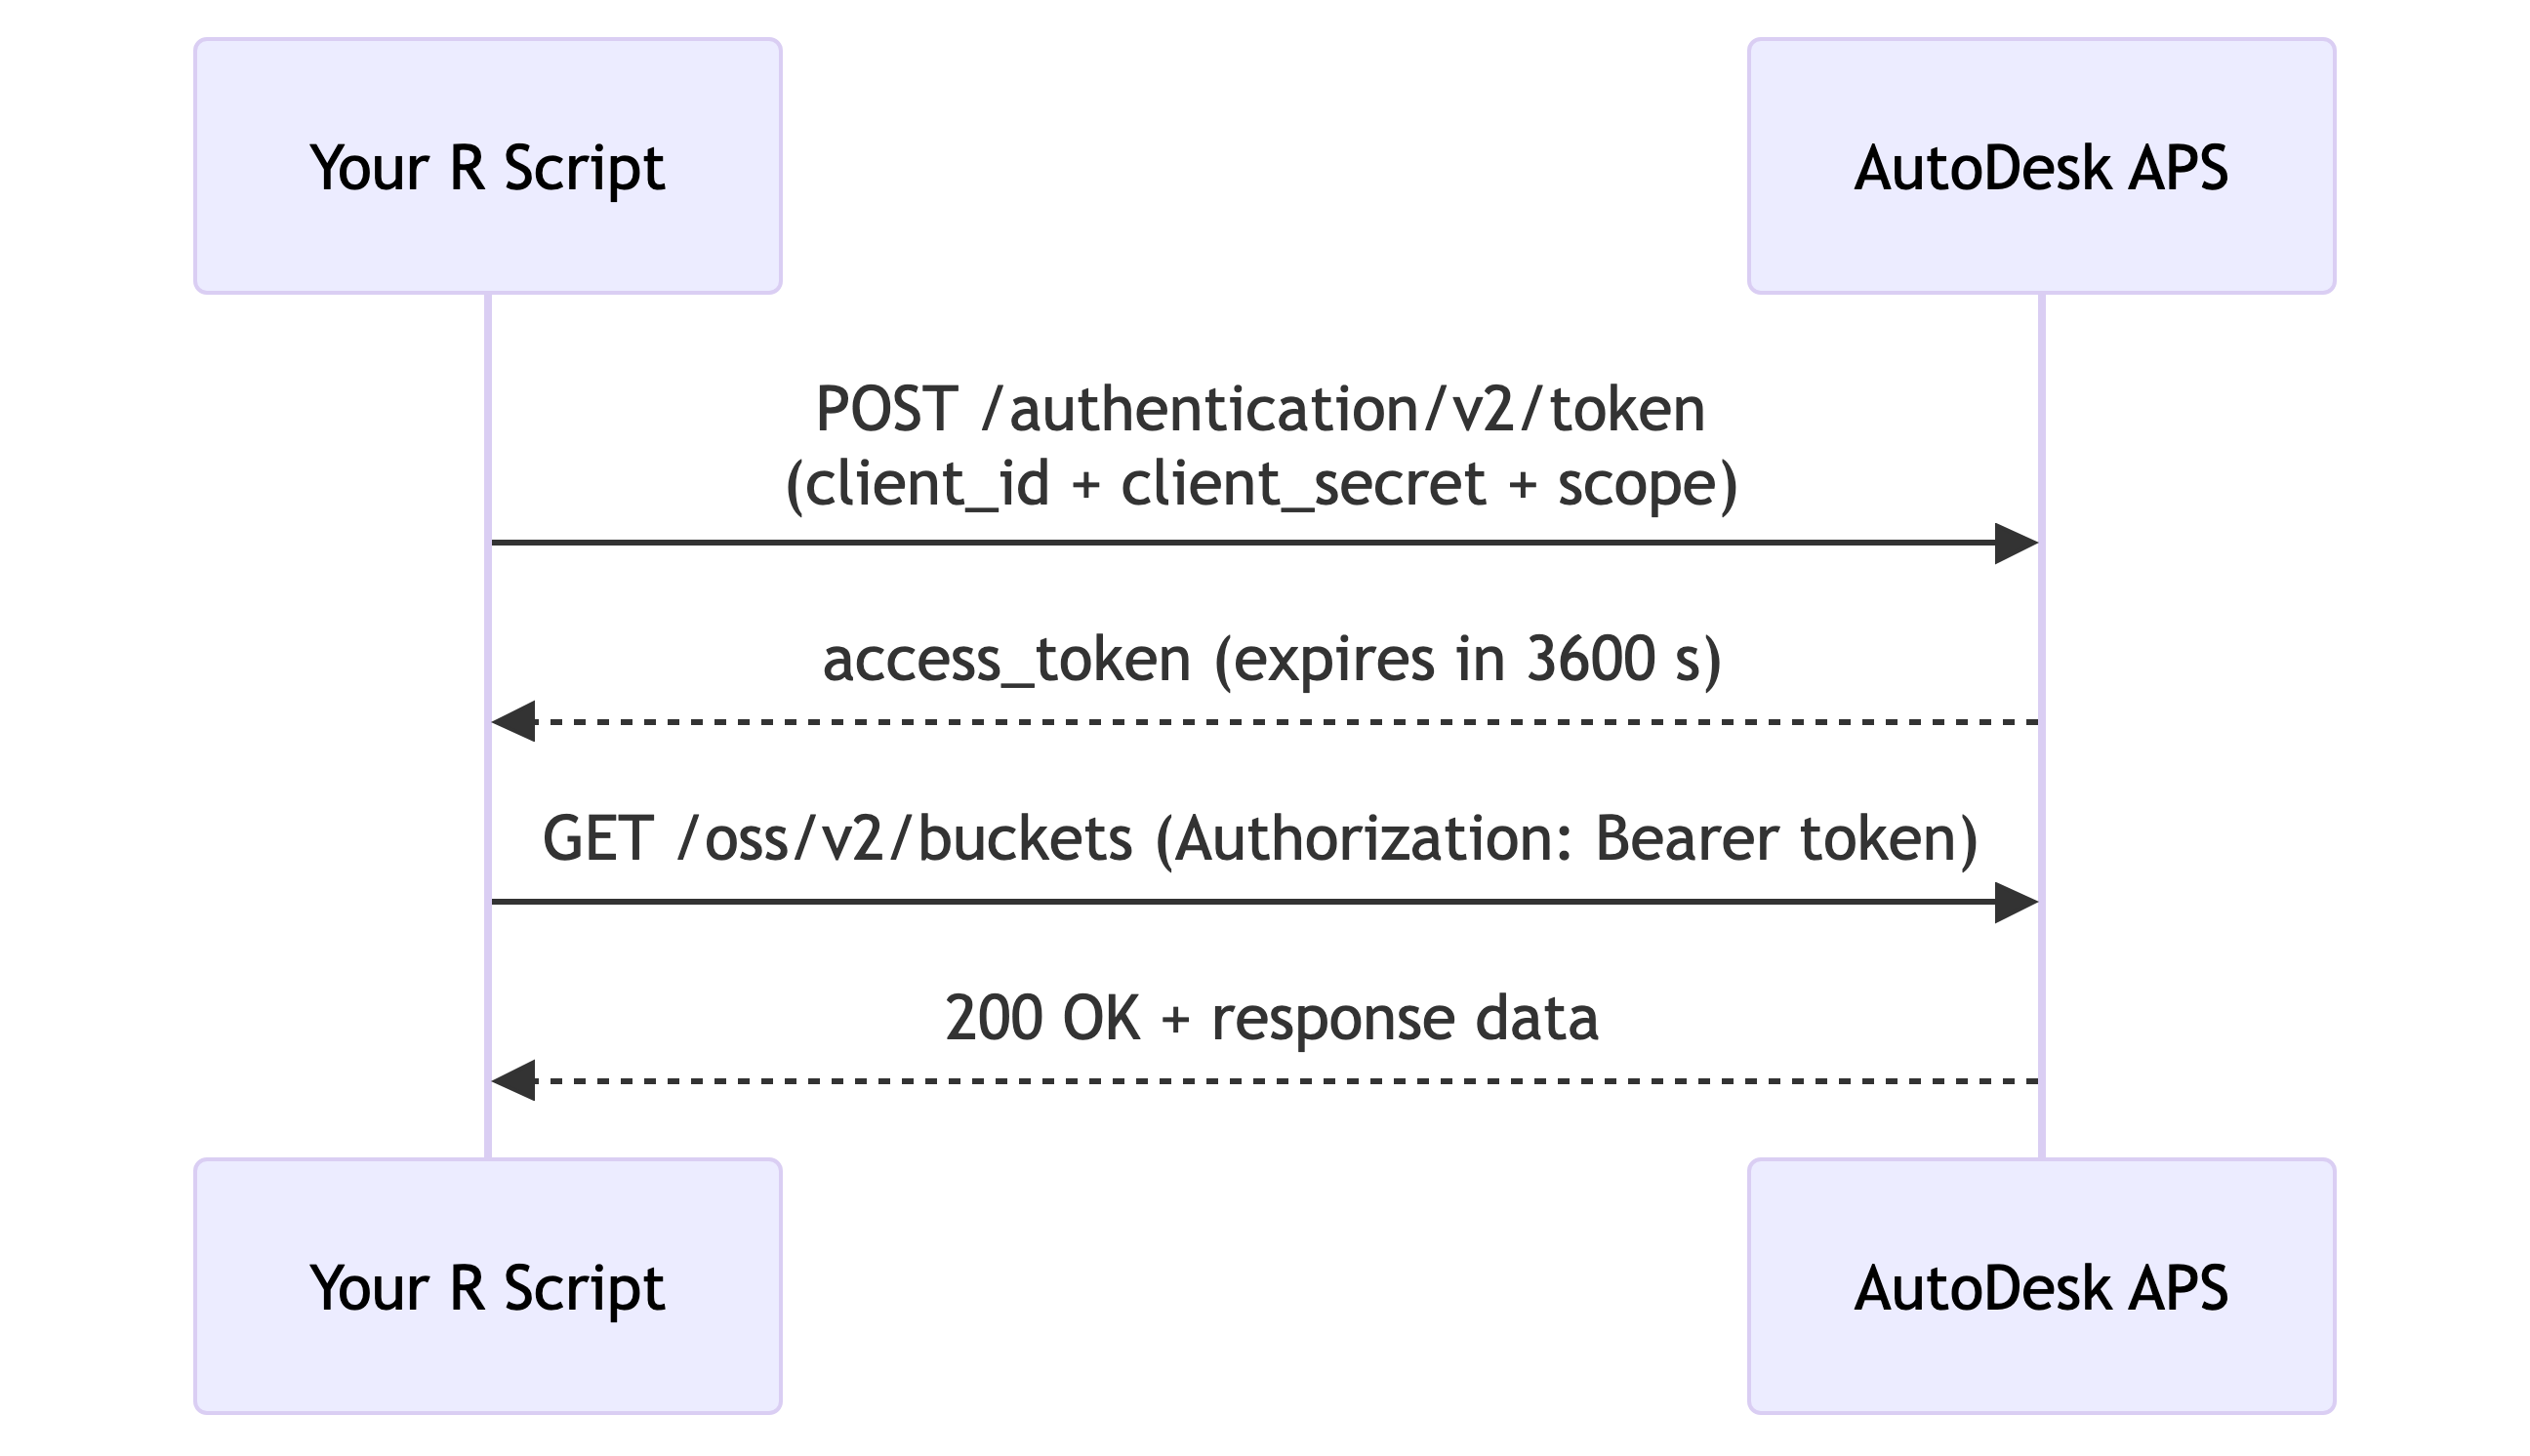
\includegraphics[width=6.75in,height=3.89in]{authentication_files/figure-latex/mermaid-figure-1.png}

\section{Store Credentials Safely}\label{store-credentials-safely}

Your Client ID and Secret are like a username and password for your app.
Keep them out of your source files and version control. The cleanest
approach in R is to stash them in \texttt{\textasciitilde{}/.Renviron}:

\begin{verbatim}
client_id = "YOUR_CLIENT_ID"
client_secret = "YOUR_CLIENT_SECRET"
token = "YOUR_ACCESS_TOKEN"
urn = "YOUR_URN"
\end{verbatim}

Reload the file without restarting R:

\begin{Shaded}
\begin{Highlighting}[]
\FunctionTok{readRenviron}\NormalTok{(}\StringTok{"\textasciitilde{}/.Renviron"}\NormalTok{)}
\end{Highlighting}
\end{Shaded}

Then pull values at runtime with \texttt{Sys.getenv()} --- credentials
never appear in your code. See
\href{https://httr2.r-lib.org/articles/wrapping-apis.html}{Wrapping
APIs} in the httr2 docs for more on this pattern.

\section{Get an Access Token}\label{get-an-access-token}

One function call does it all:

\begin{Shaded}
\begin{Highlighting}[]
\NormalTok{resp    }\OtherTok{\textless{}{-}} \FunctionTok{getToken}\NormalTok{(}\AttributeTok{id =} \FunctionTok{Sys.getenv}\NormalTok{(}\StringTok{"client\_id"}\NormalTok{), }\AttributeTok{secret =} \FunctionTok{Sys.getenv}\NormalTok{(}\StringTok{"client\_secret"}\NormalTok{))}
\NormalTok{myToken }\OtherTok{\textless{}{-}}\NormalTok{ resp}\SpecialCharTok{$}\NormalTok{content}\SpecialCharTok{$}\NormalTok{access\_token}
\NormalTok{myToken}
\CommentTok{\#\textgreater{} [1] "eyJhbGciOiJSUzI1NiIsImtpZCI6IlU3c1BKNVVpOWNaVjlIR2FhX1pIeDhEd3VYSHcifQ.}
\CommentTok{\#\textgreater{}       eyJjbGllbnRfaWQiOiJBQkNERUYxMjM0NTYiLCJleHAiOjE3NDU0MDA0MDAsInNjb3BlIjpb}
\CommentTok{\#\textgreater{}       ImRhdGE6cmVhZCJdfQ.SflKxwRJSMeKKF2QT4fwpMeJf36POk6yJV\_adQssw5c"}
\end{Highlighting}
\end{Shaded}

The full response also tells you what you're working with:

\begin{Shaded}
\begin{Highlighting}[]
\FunctionTok{str}\NormalTok{(resp}\SpecialCharTok{$}\NormalTok{content)}
\CommentTok{\#\textgreater{} List of 3}
\CommentTok{\#\textgreater{}  $ access\_token: chr "eyJhbGciOiJSUzI1NiIsImtpZCI6IlU3c1BKNVVpOWNaVjlIR..."}
\CommentTok{\#\textgreater{}  $ token\_type  : chr "Bearer"}
\CommentTok{\#\textgreater{}  $ expires\_in  : int 3600}
\end{Highlighting}
\end{Shaded}

\begin{tcolorbox}[enhanced jigsaw, titlerule=0mm, colback=white, colframe=quarto-callout-warning-color-frame, bottomtitle=1mm, bottomrule=.15mm, coltitle=black, arc=.35mm, left=2mm, title=\textcolor{quarto-callout-warning-color}{\faExclamationTriangle}\hspace{0.5em}{Warning}, colbacktitle=quarto-callout-warning-color!10!white, toptitle=1mm, breakable, toprule=.15mm, rightrule=.15mm, leftrule=.75mm, opacitybacktitle=0.6, opacityback=0]

\textbf{Tokens expire after 1 hour.} A \texttt{401\ Unauthorized}
mid-session almost always means your token timed out --- just call
\texttt{getToken()} again.

\begin{Shaded}
\begin{Highlighting}[]
\NormalTok{resp}\SpecialCharTok{$}\NormalTok{status\_code}
\CommentTok{\#\textgreater{} [1] 401}
\NormalTok{resp}\SpecialCharTok{$}\NormalTok{content}\SpecialCharTok{$}\NormalTok{errorCode}
\CommentTok{\#\textgreater{} [1] "AUTH{-}001"}
\NormalTok{resp}\SpecialCharTok{$}\NormalTok{content}\SpecialCharTok{$}\NormalTok{developerMessage}
\CommentTok{\#\textgreater{} [1] "The provided access token has expired."}
\end{Highlighting}
\end{Shaded}

\end{tcolorbox}

\section{Scopes --- Only Ask for What You
Need}\label{scopes-only-ask-for-what-you-need}

The \texttt{scope} parameter controls which APIs the token can access.
It's good practice to request the minimum scopes your task actually
requires:

\begin{longtable}[]{@{}ll@{}}
\toprule\noalign{}
Scope & What it unlocks \\
\midrule\noalign{}
\endhead
\bottomrule\noalign{}
\endlastfoot
\texttt{data:read} & Read files and derivatives \\
\texttt{data:write} & Upload and modify files \\
\texttt{data:create} & Create new files \\
\texttt{data:search} & Search within files \\
\texttt{bucket:create} & Create storage buckets \\
\texttt{bucket:read} & View bucket details \\
\texttt{bucket:update} & Modify bucket settings \\
\texttt{bucket:delete} & Delete buckets \\
\texttt{code:all} & Design Automation APIs \\
\texttt{account:read} & Read account information \\
\texttt{account:write} & Modify account settings \\
\texttt{user-profile:read} & Read user profile data \\
\end{longtable}

Pass multiple scopes as a space-separated string:

\begin{Shaded}
\begin{Highlighting}[]
\NormalTok{resp }\OtherTok{\textless{}{-}} \FunctionTok{getToken}\NormalTok{(}
  \AttributeTok{id     =} \FunctionTok{Sys.getenv}\NormalTok{(}\StringTok{"client\_id"}\NormalTok{),}
  \AttributeTok{secret =} \FunctionTok{Sys.getenv}\NormalTok{(}\StringTok{"client\_secret"}\NormalTok{),}
  \AttributeTok{scope  =} \StringTok{"bucket:create bucket:read data:write"}
\NormalTok{)}
\NormalTok{myToken }\OtherTok{\textless{}{-}}\NormalTok{ resp}\SpecialCharTok{$}\NormalTok{content}\SpecialCharTok{$}\NormalTok{access\_token}
\end{Highlighting}
\end{Shaded}

\section{Rate Limits}\label{rate-limits}

APS enforces per-application rate limits (typically 60--300 requests per
minute depending on the endpoint). Hit the ceiling and you get
\textbf{HTTP 429}:

\begin{Shaded}
\begin{Highlighting}[]
\NormalTok{resp}\SpecialCharTok{$}\NormalTok{status\_code}
\CommentTok{\#\textgreater{} [1] 429}
\NormalTok{resp}\SpecialCharTok{$}\NormalTok{content}\SpecialCharTok{$}\NormalTok{errorCode}
\CommentTok{\#\textgreater{} [1] "TOO{-}MANY{-}REQUESTS"}
\NormalTok{resp}\SpecialCharTok{$}\NormalTok{content}\SpecialCharTok{$}\NormalTok{developerMessage}
\CommentTok{\#\textgreater{} [1] "Rate limit exceeded. Retry after 60 seconds."}
\end{Highlighting}
\end{Shaded}

This simple retry helper wraps any function call that might get
rate-limited:

\begin{Shaded}
\begin{Highlighting}[]
\NormalTok{aps\_retry }\OtherTok{\textless{}{-}} \ControlFlowTok{function}\NormalTok{(fn, }\AttributeTok{max\_tries =} \DecValTok{3}\NormalTok{, }\AttributeTok{wait =} \DecValTok{10}\NormalTok{) \{}
  \ControlFlowTok{for}\NormalTok{ (i }\ControlFlowTok{in} \FunctionTok{seq\_len}\NormalTok{(max\_tries)) \{}
\NormalTok{    resp }\OtherTok{\textless{}{-}} \FunctionTok{fn}\NormalTok{()}
    \ControlFlowTok{if}\NormalTok{ (}\SpecialCharTok{!}\FunctionTok{identical}\NormalTok{(resp}\SpecialCharTok{$}\NormalTok{status\_code, }\DecValTok{429}\NormalTok{L)) }\FunctionTok{return}\NormalTok{(resp)}
    \FunctionTok{message}\NormalTok{(}\StringTok{"Rate limited — waiting "}\NormalTok{, wait, }\StringTok{"s (attempt "}\NormalTok{, i, }\StringTok{"/"}\NormalTok{, max\_tries, }\StringTok{")"}\NormalTok{)}
    \FunctionTok{Sys.sleep}\NormalTok{(wait)}
\NormalTok{  \}}
  \FunctionTok{stop}\NormalTok{(}\StringTok{"Max retries exceeded after "}\NormalTok{, max\_tries, }\StringTok{" attempts."}\NormalTok{)}
\NormalTok{\}}

\CommentTok{\# Example: poll translation status with automatic backoff}
\NormalTok{resp }\OtherTok{\textless{}{-}} \FunctionTok{aps\_retry}\NormalTok{(}\ControlFlowTok{function}\NormalTok{() }\FunctionTok{checkFile}\NormalTok{(}\AttributeTok{urn =}\NormalTok{ myEncodedUrn, }\AttributeTok{token =}\NormalTok{ myToken))}
\end{Highlighting}
\end{Shaded}

\chapter{Data Management}\label{data-management}

Think of the Data Management API as AutoDesk's cloud file system. Before
you can translate a file, embed it in a viewer, or run Design Automation
on it, the file needs to live up in APS storage. This chapter covers
everything from creating a bucket to deleting one.

The storage model is simple: your app owns \textbf{buckets}, and buckets
hold \textbf{objects} (your files).

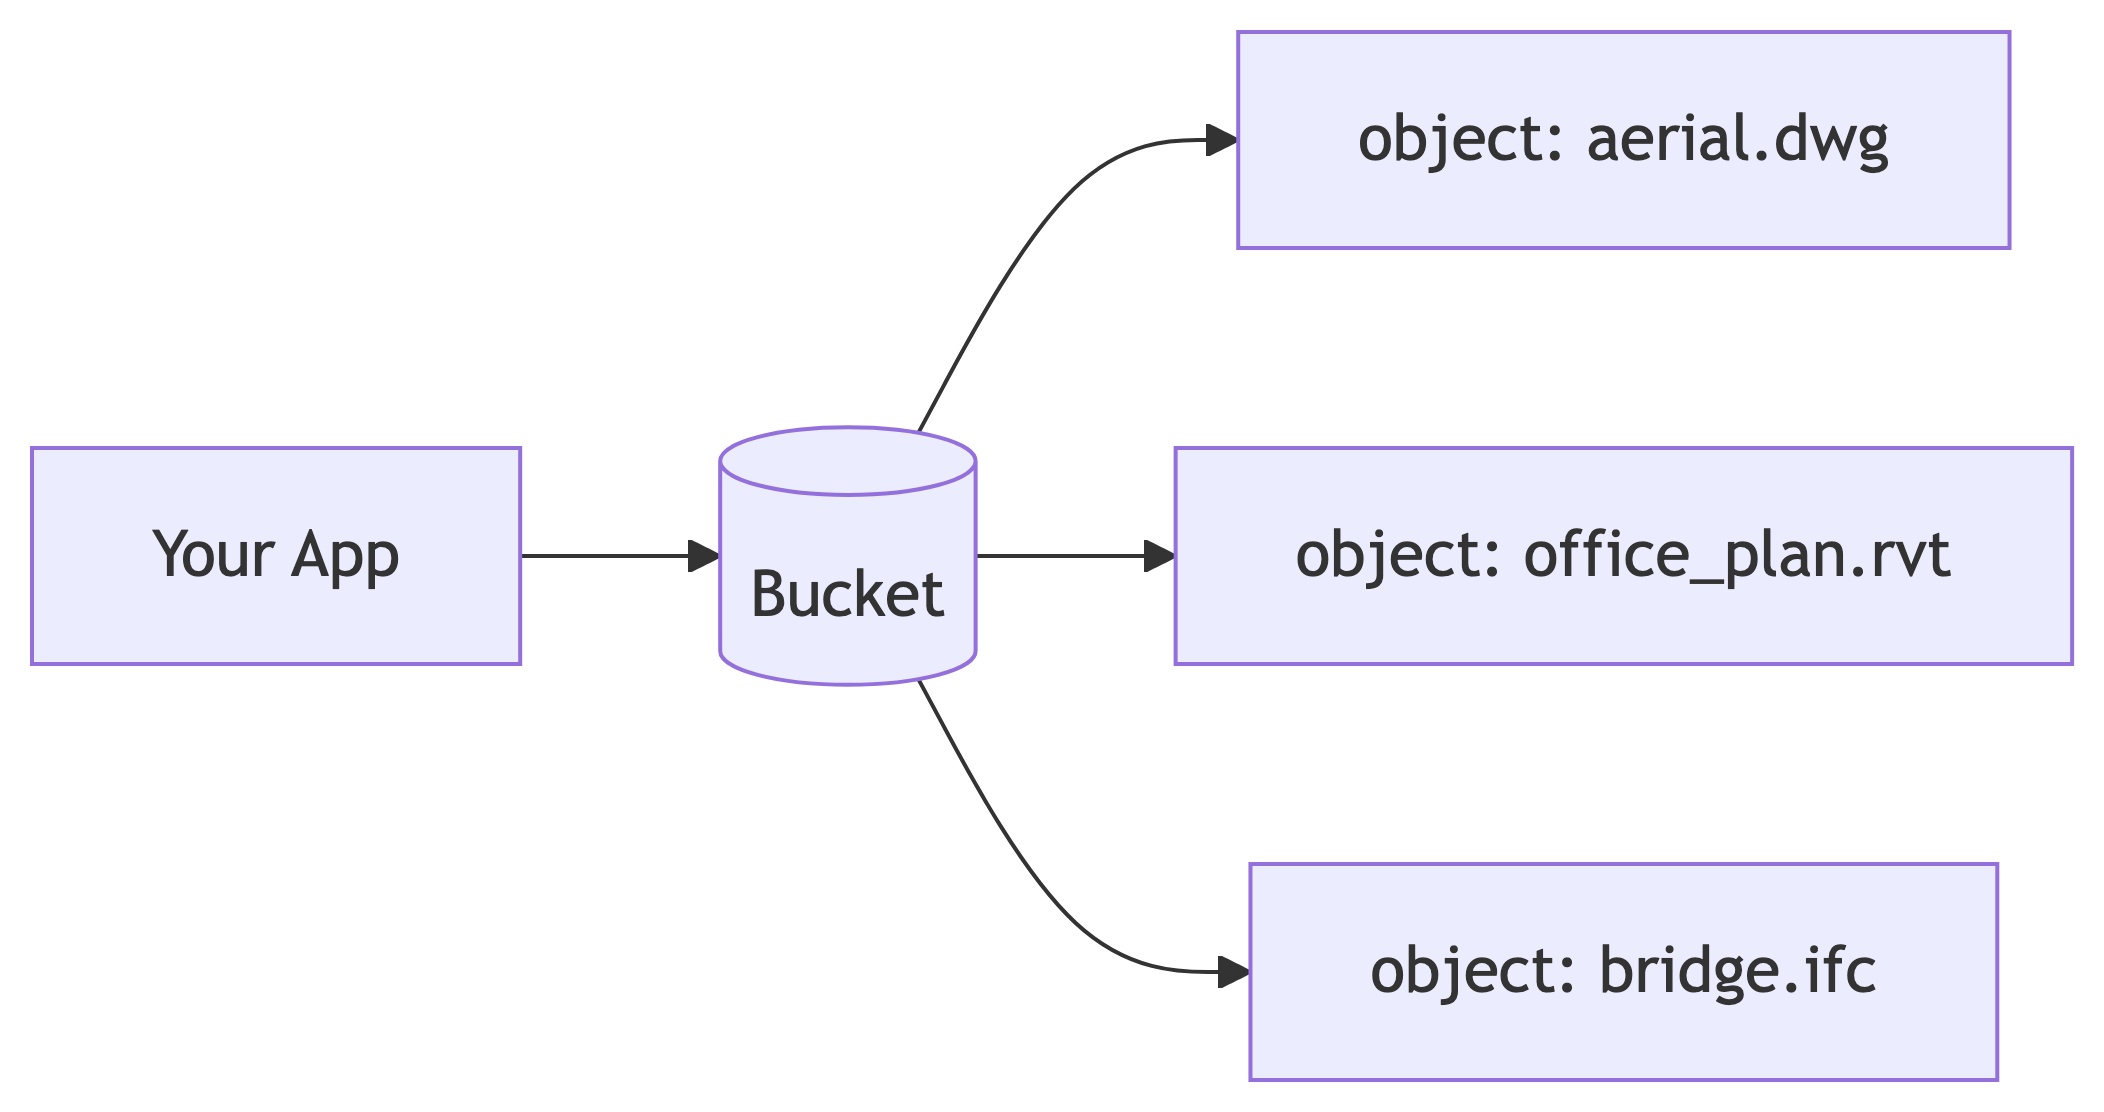
\includegraphics[width=5.48in,height=2.9in]{data-management_files/figure-latex/mermaid-figure-1.png}

\section{Create a Bucket}\label{create-a-bucket}

Get a token first - bucket creation needs \texttt{bucket:create} and
\texttt{bucket:read} scopes at minimum:

\begin{Shaded}
\begin{Highlighting}[]
\NormalTok{resp }\OtherTok{\textless{}{-}} \FunctionTok{getToken}\NormalTok{(}
  \AttributeTok{id     =} \FunctionTok{Sys.getenv}\NormalTok{(}\StringTok{"client\_id"}\NormalTok{),}
  \AttributeTok{secret =} \FunctionTok{Sys.getenv}\NormalTok{(}\StringTok{"client\_secret"}\NormalTok{),}
  \AttributeTok{scope  =} \StringTok{"bucket:create bucket:read data:write"}
\NormalTok{)}
\NormalTok{myToken }\OtherTok{\textless{}{-}}\NormalTok{ resp}\SpecialCharTok{$}\NormalTok{content}\SpecialCharTok{$}\NormalTok{access\_token}
\CommentTok{\#\textgreater{} [1] "eyJhbGciOiJSUzI1NiIsImtpZCI6IlU3c1BKNVVpOWNaVjlIR2FhX1pIeDhEd3VYSHcifQ..."}
\end{Highlighting}
\end{Shaded}

Bucket retention policy controls how long your objects stick around:

\begin{longtable}[]{@{}ll@{}}
\toprule\noalign{}
Policy & Files live for \\
\midrule\noalign{}
\endhead
\bottomrule\noalign{}
\endlastfoot
\texttt{"transient"} & 24 hours (great for testing) \\
\texttt{"temporary"} & 30 days \\
\texttt{"persistent"} & Until you delete them \\
\end{longtable}

\begin{tcolorbox}[enhanced jigsaw, titlerule=0mm, colback=white, colframe=quarto-callout-warning-color-frame, bottomtitle=1mm, bottomrule=.15mm, coltitle=black, arc=.35mm, left=2mm, title=\textcolor{quarto-callout-warning-color}{\faExclamationTriangle}\hspace{0.5em}{Warning}, colbacktitle=quarto-callout-warning-color!10!white, toptitle=1mm, breakable, toprule=.15mm, rightrule=.15mm, leftrule=.75mm, opacitybacktitle=0.6, opacityback=0]

\textbf{Bucket names are globally unique} --- not just within your app,
but across every APS application everywhere. A name like \texttt{"test"}
is long gone. Use something specific to your organisation and project,
e.g.~\texttt{"acmecorp-bridge-analysis-prod"}. A duplicate name returns
a \texttt{409\ Conflict}:

\begin{Shaded}
\begin{Highlighting}[]
\NormalTok{resp}\SpecialCharTok{$}\NormalTok{status\_code}
\CommentTok{\#\textgreater{} [1] 409}
\NormalTok{resp}\SpecialCharTok{$}\NormalTok{content}\SpecialCharTok{$}\NormalTok{reason}
\CommentTok{\#\textgreater{} [1] "Bucket already exists"}
\end{Highlighting}
\end{Shaded}

\end{tcolorbox}

\begin{Shaded}
\begin{Highlighting}[]
\NormalTok{resp }\OtherTok{\textless{}{-}} \FunctionTok{makeBucket}\NormalTok{(}\AttributeTok{token =}\NormalTok{ myToken, }\AttributeTok{bucket =} \StringTok{"mybucket"}\NormalTok{, }\AttributeTok{policy =} \StringTok{"persistent"}\NormalTok{)}
\NormalTok{resp}\SpecialCharTok{$}\NormalTok{content}
\CommentTok{\#\textgreater{} $bucketKey}
\CommentTok{\#\textgreater{} [1] "mybucket"}
\CommentTok{\#\textgreater{}}
\CommentTok{\#\textgreater{} $bucketOwner}
\CommentTok{\#\textgreater{} [1] "3MVG99OxTyEMCQ3gNp2PjtXbmT8T\_MnfCTtpQkuiJNxGtXuoKP7"}
\CommentTok{\#\textgreater{}}
\CommentTok{\#\textgreater{} $createdDate}
\CommentTok{\#\textgreater{} [1] 1745356800000}
\CommentTok{\#\textgreater{}}
\CommentTok{\#\textgreater{} $policyKey}
\CommentTok{\#\textgreater{} [1] "persistent"}
\end{Highlighting}
\end{Shaded}

Check on a bucket anytime with \texttt{checkBucket()}:

\begin{Shaded}
\begin{Highlighting}[]
\NormalTok{resp }\OtherTok{\textless{}{-}} \FunctionTok{checkBucket}\NormalTok{(}\AttributeTok{token =}\NormalTok{ myToken, }\AttributeTok{bucket =} \StringTok{"mybucket"}\NormalTok{)}
\NormalTok{resp}\SpecialCharTok{$}\NormalTok{content}\SpecialCharTok{$}\NormalTok{policyKey}
\CommentTok{\#\textgreater{} [1] "persistent"}
\end{Highlighting}
\end{Shaded}

\section{Upload a File}\label{upload-a-file}

\texttt{uploadFile()} handles files up to 100 MB. It returns the
object's \texttt{objectId}, a URN that every other API will ask for, so
save it somewhere handy:

\begin{Shaded}
\begin{Highlighting}[]
\NormalTok{resp  }\OtherTok{\textless{}{-}} \FunctionTok{uploadFile}\NormalTok{(}
  \AttributeTok{file   =} \FunctionTok{system.file}\NormalTok{(}\StringTok{"samples/aerial.dwg"}\NormalTok{, }\AttributeTok{package =} \StringTok{"AutoDeskR"}\NormalTok{),}
  \AttributeTok{token  =}\NormalTok{ myToken,}
  \AttributeTok{bucket =} \StringTok{"mybucket"}
\NormalTok{)}
\NormalTok{myUrn }\OtherTok{\textless{}{-}}\NormalTok{ resp}\SpecialCharTok{$}\NormalTok{content}\SpecialCharTok{$}\NormalTok{objectId}
\NormalTok{resp}\SpecialCharTok{$}\NormalTok{content}
\CommentTok{\#\textgreater{} $bucketKey}
\CommentTok{\#\textgreater{} [1] "mybucket"}
\CommentTok{\#\textgreater{}}
\CommentTok{\#\textgreater{} $objectId}
\CommentTok{\#\textgreater{} [1] "urn:adsk.objects:os.object:mybucket/aerial.dwg"}
\CommentTok{\#\textgreater{}}
\CommentTok{\#\textgreater{} $objectKey}
\CommentTok{\#\textgreater{} [1] "aerial.dwg"}
\CommentTok{\#\textgreater{}}
\CommentTok{\#\textgreater{} $size}
\CommentTok{\#\textgreater{} [1] 3145728}
\CommentTok{\#\textgreater{}}
\CommentTok{\#\textgreater{} $contentType}
\CommentTok{\#\textgreater{} [1] "application/octet{-}stream"}
\CommentTok{\#\textgreater{}}
\CommentTok{\#\textgreater{} $location}
\CommentTok{\#\textgreater{} [1] "https://developer.api.autodesk.com/oss/v2/buckets/mybucket/objects/aerial.dwg"}
\end{Highlighting}
\end{Shaded}

\subsection{Big Files (\textgreater{} 100 MB)}\label{big-files-100-mb}

For anything over 100 MB, use \texttt{uploadFileSigned()}. iI routes the
transfer through signed S3 URLs to sidestep timeout limits:

\begin{Shaded}
\begin{Highlighting}[]
\NormalTok{resp  }\OtherTok{\textless{}{-}} \FunctionTok{uploadFileSigned}\NormalTok{(}
  \AttributeTok{file   =} \StringTok{"path/to/large\_model.rvt"}\NormalTok{,}
  \AttributeTok{token  =}\NormalTok{ myToken,}
  \AttributeTok{bucket =} \StringTok{"mybucket"}
\NormalTok{)}
\NormalTok{myUrn }\OtherTok{\textless{}{-}}\NormalTok{ resp}\SpecialCharTok{$}\NormalTok{content}\SpecialCharTok{$}\NormalTok{objectId}
\NormalTok{resp}\SpecialCharTok{$}\NormalTok{content}\SpecialCharTok{$}\NormalTok{size}
\CommentTok{\#\textgreater{} [1] 524288000}
\end{Highlighting}
\end{Shaded}

\section{List Buckets and Objects}\label{list-buckets-and-objects}

See all buckets your app owns. Paginate with \texttt{limit} and
\texttt{startAt}:

\begin{Shaded}
\begin{Highlighting}[]
\NormalTok{resp }\OtherTok{\textless{}{-}} \FunctionTok{listBuckets}\NormalTok{(}\AttributeTok{token =}\NormalTok{ myToken, }\AttributeTok{limit =} \DecValTok{10}\NormalTok{)}
\NormalTok{resp}\SpecialCharTok{$}\NormalTok{content}\SpecialCharTok{$}\NormalTok{items}
\CommentTok{\#\textgreater{}                          bucketKey    createdDate  policyKey}
\CommentTok{\#\textgreater{} 1                       mybucket  1745356800000 persistent}
\CommentTok{\#\textgreater{} 2                  archive{-}2025  1740000000000  temporary}
\CommentTok{\#\textgreater{} 3              visualization{-}dev  1738000000000  transient}

\CommentTok{\# Next page}
\NormalTok{resp }\OtherTok{\textless{}{-}} \FunctionTok{listBuckets}\NormalTok{(}\AttributeTok{token =}\NormalTok{ myToken, }\AttributeTok{limit =} \DecValTok{10}\NormalTok{, }\AttributeTok{startAt =} \StringTok{"visualization{-}dev"}\NormalTok{)}
\end{Highlighting}
\end{Shaded}

Filter by region if your app spans geographies:

\begin{Shaded}
\begin{Highlighting}[]
\NormalTok{resp }\OtherTok{\textless{}{-}} \FunctionTok{listBuckets}\NormalTok{(}\AttributeTok{token =}\NormalTok{ myToken, }\AttributeTok{region =} \StringTok{"EMEA"}\NormalTok{)}
\NormalTok{resp}\SpecialCharTok{$}\NormalTok{content}\SpecialCharTok{$}\NormalTok{items}
\CommentTok{\#\textgreater{}       bucketKey    createdDate  policyKey}
\CommentTok{\#\textgreater{} 1  emea{-}models  1742000000000 persistent}
\end{Highlighting}
\end{Shaded}

List the files inside a bucket:

\begin{Shaded}
\begin{Highlighting}[]
\NormalTok{resp }\OtherTok{\textless{}{-}} \FunctionTok{listObjects}\NormalTok{(}\AttributeTok{token =}\NormalTok{ myToken, }\AttributeTok{bucket =} \StringTok{"mybucket"}\NormalTok{, }\AttributeTok{limit =} \DecValTok{10}\NormalTok{)}
\NormalTok{resp}\SpecialCharTok{$}\NormalTok{content}\SpecialCharTok{$}\NormalTok{items}
\CommentTok{\#\textgreater{}          objectKey                                              objectId     size}
\CommentTok{\#\textgreater{} 1       aerial.dwg  urn:adsk.objects:os.object:mybucket/aerial.dwg      3145728}
\CommentTok{\#\textgreater{} 2  office\_plan.rvt  urn:adsk.objects:os.object:mybucket/office\_plan.rvt 52428800}
\CommentTok{\#\textgreater{} 3      bridge.ifc   urn:adsk.objects:os.object:mybucket/bridge.ifc       8388608}
\end{Highlighting}
\end{Shaded}

\section{Delete Objects and Buckets}\label{delete-objects-and-buckets}

Remove a specific file:

\begin{Shaded}
\begin{Highlighting}[]
\NormalTok{resp }\OtherTok{\textless{}{-}} \FunctionTok{deleteObject}\NormalTok{(}\AttributeTok{token =}\NormalTok{ myToken, }\AttributeTok{bucket =} \StringTok{"mybucket"}\NormalTok{, }\AttributeTok{object =} \StringTok{"aerial.dwg"}\NormalTok{)}
\NormalTok{resp}\SpecialCharTok{$}\NormalTok{status\_code}
\CommentTok{\#\textgreater{} [1] 200}
\end{Highlighting}
\end{Shaded}

Remove the whole bucket:

\begin{Shaded}
\begin{Highlighting}[]
\NormalTok{resp }\OtherTok{\textless{}{-}} \FunctionTok{deleteBucket}\NormalTok{(}\AttributeTok{token =}\NormalTok{ myToken, }\AttributeTok{bucket =} \StringTok{"mybucket"}\NormalTok{)}
\NormalTok{resp}\SpecialCharTok{$}\NormalTok{status\_code}
\CommentTok{\#\textgreater{} [1] 200}
\end{Highlighting}
\end{Shaded}

\begin{tcolorbox}[enhanced jigsaw, titlerule=0mm, colback=white, colframe=quarto-callout-warning-color-frame, bottomtitle=1mm, bottomrule=.15mm, coltitle=black, arc=.35mm, left=2mm, title=\textcolor{quarto-callout-warning-color}{\faExclamationTriangle}\hspace{0.5em}{Warning}, colbacktitle=quarto-callout-warning-color!10!white, toptitle=1mm, breakable, toprule=.15mm, rightrule=.15mm, leftrule=.75mm, opacitybacktitle=0.6, opacityback=0]

\textbf{Empty the bucket first.} \texttt{deleteBucket()} won't touch a
bucket that still has objects in it. Delete everything with
\texttt{deleteObject()} first, or you'll get:

\begin{Shaded}
\begin{Highlighting}[]
\NormalTok{resp}\SpecialCharTok{$}\NormalTok{status\_code}
\CommentTok{\#\textgreater{} [1] 409}
\NormalTok{resp}\SpecialCharTok{$}\NormalTok{content}\SpecialCharTok{$}\NormalTok{reason}
\CommentTok{\#\textgreater{} [1] "Bucket not empty"}
\end{Highlighting}
\end{Shaded}

\end{tcolorbox}

\chapter{Model Derivative}\label{model-derivative}

A DWG file sitting in a bucket is just bytes. The Model Derivative API
is what turns those bytes into something useful, OBJ and STL meshes you
can analyse in R, SVF viewables you can embed in a browser, or
structured metadata you can query with \texttt{dplyr}. This chapter
covers the full translation workflow.

The pattern is always the same: submit a job, poll until it finishes,
then pull the output.

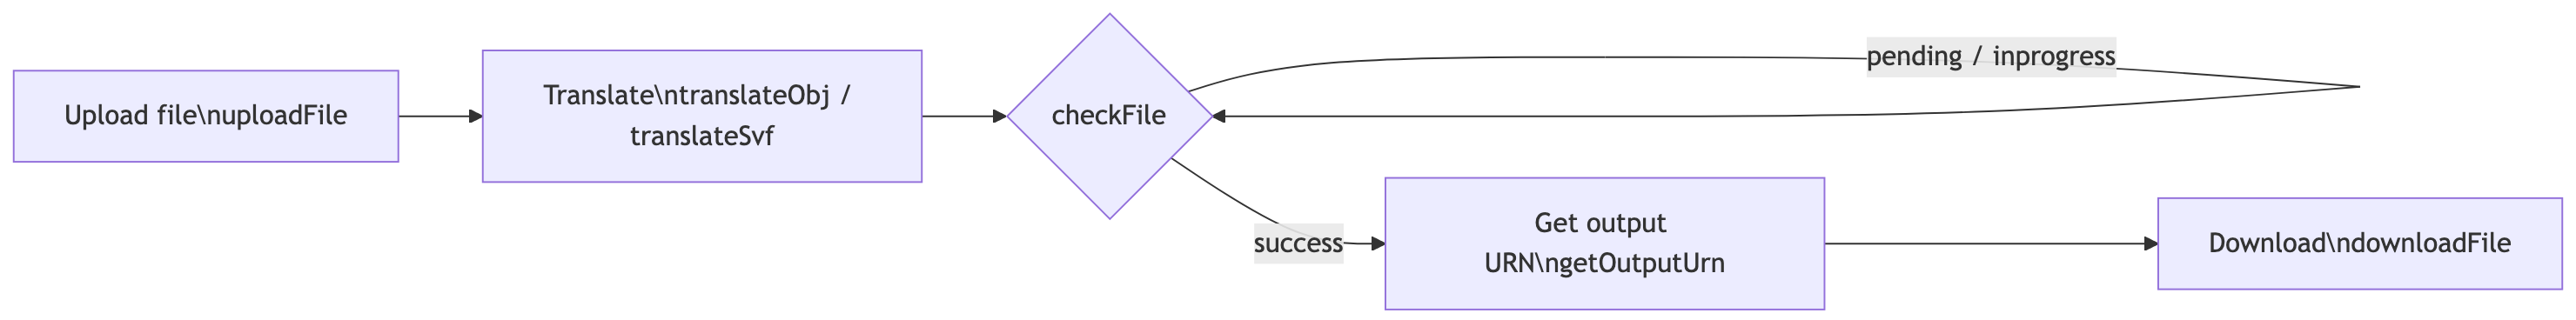
\includegraphics[width=15.89in,height=1.99in]{model-derivative_files/figure-latex/mermaid-figure-1.png}

\section{Translate to OBJ}\label{translate-to-obj}

First get a token with \texttt{data:read} and \texttt{data:write}
scopes. Note that only certain source formats can produce OBJ output
(DWG, IPT, IAM, IPN, F3D, FBX. See the
\href{https://aps.autodesk.com/en/docs/model-derivative/v2/developers_guide/supported-translations/}{APS
supported formats list} for the full matrix).

\begin{Shaded}
\begin{Highlighting}[]
\NormalTok{resp }\OtherTok{\textless{}{-}} \FunctionTok{getToken}\NormalTok{(}
  \AttributeTok{id     =} \FunctionTok{Sys.getenv}\NormalTok{(}\StringTok{"client\_id"}\NormalTok{),}
  \AttributeTok{secret =} \FunctionTok{Sys.getenv}\NormalTok{(}\StringTok{"client\_secret"}\NormalTok{),}
  \AttributeTok{scope  =} \StringTok{"data:read data:write"}
\NormalTok{)}
\NormalTok{myToken }\OtherTok{\textless{}{-}}\NormalTok{ resp}\SpecialCharTok{$}\NormalTok{content}\SpecialCharTok{$}\NormalTok{access\_token}
\end{Highlighting}
\end{Shaded}

APS requires the file's URN to be Base-64 encoded before it'll accept it
--- \texttt{jsonlite::base64\_enc()} handles that:

\begin{Shaded}
\begin{Highlighting}[]
\NormalTok{myEncodedUrn }\OtherTok{\textless{}{-}}\NormalTok{ jsonlite}\SpecialCharTok{::}\FunctionTok{base64\_enc}\NormalTok{(myUrn)}
\NormalTok{myEncodedUrn}
\CommentTok{\#\textgreater{} [1] "dXJuOmFkc2sub2JqZWN0czpvcy5vYmplY3Q6bXlidWNrZXQvYWVyaWFsLmR3Zw=="}
\end{Highlighting}
\end{Shaded}

Kick off the translation:

\begin{Shaded}
\begin{Highlighting}[]
\NormalTok{resp }\OtherTok{\textless{}{-}} \FunctionTok{translateObj}\NormalTok{(}\AttributeTok{urn =}\NormalTok{ myEncodedUrn, }\AttributeTok{token =}\NormalTok{ myToken)}
\NormalTok{resp}\SpecialCharTok{$}\NormalTok{content}
\CommentTok{\#\textgreater{} $result}
\CommentTok{\#\textgreater{} [1] "created"}
\CommentTok{\#\textgreater{}}
\CommentTok{\#\textgreater{} $urn}
\CommentTok{\#\textgreater{} [1] "dXJuOmFkc2sub2JqZWN0czpvcy5vYmplY3Q6bXlidWNrZXQvYWVyaWFsLmR3Zw=="}
\CommentTok{\#\textgreater{}}
\CommentTok{\#\textgreater{} $acceptedJobs$output$formats[[1]]$type}
\CommentTok{\#\textgreater{} [1] "obj"}
\end{Highlighting}
\end{Shaded}

\begin{tcolorbox}[enhanced jigsaw, titlerule=0mm, colback=white, colframe=quarto-callout-warning-color-frame, bottomtitle=1mm, bottomrule=.15mm, coltitle=black, arc=.35mm, left=2mm, title=\textcolor{quarto-callout-warning-color}{\faExclamationTriangle}\hspace{0.5em}{Warning}, colbacktitle=quarto-callout-warning-color!10!white, toptitle=1mm, breakable, toprule=.15mm, rightrule=.15mm, leftrule=.75mm, opacitybacktitle=0.6, opacityback=0]

\textbf{OBJ translation only accepts certain source formats.} Submitting
an unsupported format returns a \texttt{415\ Unsupported\ Media\ Type}:

\begin{Shaded}
\begin{Highlighting}[]
\NormalTok{resp}\SpecialCharTok{$}\NormalTok{status\_code}
\CommentTok{\#\textgreater{} [1] 415}
\NormalTok{resp}\SpecialCharTok{$}\NormalTok{content}\SpecialCharTok{$}\NormalTok{diagnostic}
\CommentTok{\#\textgreater{} [1] "File type not supported for OBJ translation."}
\end{Highlighting}
\end{Shaded}

\end{tcolorbox}

Poll \texttt{checkFile()} until \texttt{status} hits \texttt{"success"}.
The job can take anywhere from a few seconds to a few minutes depending
on file complexity:

\begin{Shaded}
\begin{Highlighting}[]
\NormalTok{resp }\OtherTok{\textless{}{-}} \FunctionTok{checkFile}\NormalTok{(}\AttributeTok{urn =}\NormalTok{ myEncodedUrn, }\AttributeTok{token =}\NormalTok{ myToken)}
\NormalTok{resp}\SpecialCharTok{$}\NormalTok{content}
\CommentTok{\#\textgreater{} $status}
\CommentTok{\#\textgreater{} [1] "success"}
\CommentTok{\#\textgreater{}}
\CommentTok{\#\textgreater{} $progress}
\CommentTok{\#\textgreater{} [1] "complete"}
\CommentTok{\#\textgreater{}}
\CommentTok{\#\textgreater{} $region}
\CommentTok{\#\textgreater{} [1] "US"}
\end{Highlighting}
\end{Shaded}

\begin{tcolorbox}[enhanced jigsaw, titlerule=0mm, colback=white, colframe=quarto-callout-note-color-frame, bottomtitle=1mm, bottomrule=.15mm, coltitle=black, arc=.35mm, left=2mm, title=\textcolor{quarto-callout-note-color}{\faInfo}\hspace{0.5em}{Note}, colbacktitle=quarto-callout-note-color!10!white, toptitle=1mm, breakable, toprule=.15mm, rightrule=.15mm, leftrule=.75mm, opacitybacktitle=0.6, opacityback=0]

Translation status moves through \texttt{"pending"} →
\texttt{"inprogress"} → \texttt{"success"}. Don't try to download before
you see \texttt{"success"} --- there's nothing there yet. Use the
\texttt{aps\_retry()} helper from the
\hyperref[rate-limits]{Authentication} chapter to handle rate limiting
while you wait.

\end{tcolorbox}

Retrieve the output URN, then download:

\begin{Shaded}
\begin{Highlighting}[]
\NormalTok{resp }\OtherTok{\textless{}{-}} \FunctionTok{getOutputUrn}\NormalTok{(}\AttributeTok{urn =}\NormalTok{ myUrn, }\AttributeTok{token =} \FunctionTok{Sys.getenv}\NormalTok{(}\StringTok{"token"}\NormalTok{))}
\NormalTok{myOutputUrn        }\OtherTok{\textless{}{-}}\NormalTok{ resp}\SpecialCharTok{$}\NormalTok{content}\SpecialCharTok{$}\NormalTok{derivatives[[}\DecValTok{1}\NormalTok{]]}\SpecialCharTok{$}\NormalTok{children[[}\DecValTok{1}\NormalTok{]]}\SpecialCharTok{$}\NormalTok{urn}
\NormalTok{myEncodedOutputUrn }\OtherTok{\textless{}{-}}\NormalTok{ jsonlite}\SpecialCharTok{::}\FunctionTok{base64\_enc}\NormalTok{(myOutputUrn)}

\NormalTok{resp }\OtherTok{\textless{}{-}} \FunctionTok{downloadFile}\NormalTok{(}
  \AttributeTok{urn        =}\NormalTok{ myEncodedUrn,}
  \AttributeTok{output\_urn =}\NormalTok{ myEncodedOutputUrn,}
  \AttributeTok{token      =}\NormalTok{ myToken,}
  \AttributeTok{destfile   =} \StringTok{"aerial.obj"}
\NormalTok{)}
\NormalTok{resp}\SpecialCharTok{$}\NormalTok{status\_code}
\CommentTok{\#\textgreater{} [1] 200}
\end{Highlighting}
\end{Shaded}

\section{Translate to STL}\label{translate-to-stl}

Same pattern as OBJ, different function:

\begin{Shaded}
\begin{Highlighting}[]
\NormalTok{resp }\OtherTok{\textless{}{-}} \FunctionTok{translateStl}\NormalTok{(}\AttributeTok{urn =}\NormalTok{ myEncodedUrn, }\AttributeTok{token =}\NormalTok{ myToken)}
\NormalTok{resp}\SpecialCharTok{$}\NormalTok{content}\SpecialCharTok{$}\NormalTok{acceptedJobs}\SpecialCharTok{$}\NormalTok{output}\SpecialCharTok{$}\NormalTok{formats[[}\DecValTok{1}\NormalTok{]]}\SpecialCharTok{$}\NormalTok{type}
\CommentTok{\#\textgreater{} [1] "stl"}

\CommentTok{\# Poll until done}
\NormalTok{resp }\OtherTok{\textless{}{-}} \FunctionTok{checkFile}\NormalTok{(}\AttributeTok{urn =}\NormalTok{ myEncodedUrn, }\AttributeTok{token =}\NormalTok{ myToken)}
\NormalTok{resp}\SpecialCharTok{$}\NormalTok{content}\SpecialCharTok{$}\NormalTok{status}
\CommentTok{\#\textgreater{} [1] "success"}
\end{Highlighting}
\end{Shaded}

\section{Extract Metadata from a
File}\label{extract-metadata-from-a-file}

SVF format unlocks the structured metadata inside a model. The object
tree, property sets, layer information. This is the format the Viewer
also uses.

\begin{Shaded}
\begin{Highlighting}[]
\NormalTok{resp }\OtherTok{\textless{}{-}} \FunctionTok{translateSvf}\NormalTok{(}\AttributeTok{urn =}\NormalTok{ myEncodedUrn, }\AttributeTok{token =}\NormalTok{ myToken)}
\NormalTok{resp}\SpecialCharTok{$}\NormalTok{content}\SpecialCharTok{$}\NormalTok{result}
\CommentTok{\#\textgreater{} [1] "created"}

\CommentTok{\# Wait for it...}
\NormalTok{resp }\OtherTok{\textless{}{-}} \FunctionTok{checkFile}\NormalTok{(}\AttributeTok{urn =}\NormalTok{ myEncodedUrn, }\AttributeTok{token =}\NormalTok{ myToken)}
\NormalTok{resp}\SpecialCharTok{$}\NormalTok{content}\SpecialCharTok{$}\NormalTok{status}
\CommentTok{\#\textgreater{} [1] "success"}
\end{Highlighting}
\end{Shaded}

\texttt{getMetadata()} returns the viewable GUIDs. You'll need the GUID
for every subsequent metadata call:

\begin{Shaded}
\begin{Highlighting}[]
\NormalTok{resp   }\OtherTok{\textless{}{-}} \FunctionTok{getMetadata}\NormalTok{(}\AttributeTok{urn =}\NormalTok{ myEncodedUrn, }\AttributeTok{token =}\NormalTok{ myToken)}
\NormalTok{myGuid }\OtherTok{\textless{}{-}}\NormalTok{ resp}\SpecialCharTok{$}\NormalTok{content}\SpecialCharTok{$}\NormalTok{data}\SpecialCharTok{$}\NormalTok{metadata[[}\DecValTok{1}\NormalTok{]]}\SpecialCharTok{$}\NormalTok{guid}
\NormalTok{resp}\SpecialCharTok{$}\NormalTok{content}\SpecialCharTok{$}\NormalTok{data}
\CommentTok{\#\textgreater{} $type}
\CommentTok{\#\textgreater{} [1] "metadata"}
\CommentTok{\#\textgreater{}}
\CommentTok{\#\textgreater{} $metadata[[1]]$name}
\CommentTok{\#\textgreater{} [1] "aerial"}
\CommentTok{\#\textgreater{}}
\CommentTok{\#\textgreater{} $metadata[[1]]$guid}
\CommentTok{\#\textgreater{} [1] "a7b3c9d2{-}4e1f{-}4a8b{-}b6c2{-}9d3e7f5a1b4c"}
\CommentTok{\#\textgreater{}}
\CommentTok{\#\textgreater{} $metadata[[1]]$isMasterView}
\CommentTok{\#\textgreater{} [1] TRUE}
\end{Highlighting}
\end{Shaded}

\texttt{getObjectTree()} returns the model's full object hierarchy. For
a DWG, the children of the root node are its layers:

\begin{Shaded}
\begin{Highlighting}[]
\NormalTok{resp }\OtherTok{\textless{}{-}} \FunctionTok{getObjectTree}\NormalTok{(}\AttributeTok{guid =}\NormalTok{ myGuid, }\AttributeTok{urn =}\NormalTok{ myEncodedUrn, }\AttributeTok{token =}\NormalTok{ myToken)}
\NormalTok{resp}\SpecialCharTok{$}\NormalTok{content}\SpecialCharTok{$}\NormalTok{data}\SpecialCharTok{$}\NormalTok{objects[[}\DecValTok{1}\NormalTok{]]}
\CommentTok{\#\textgreater{} $objectid}
\CommentTok{\#\textgreater{} [1] 1}
\CommentTok{\#\textgreater{}}
\CommentTok{\#\textgreater{} $name}
\CommentTok{\#\textgreater{} [1] "aerial.dwg"}
\CommentTok{\#\textgreater{}}
\CommentTok{\#\textgreater{} $objects[[1]]$name}
\CommentTok{\#\textgreater{} [1] "Layer: A{-}SITE"}
\CommentTok{\#\textgreater{}}
\CommentTok{\#\textgreater{} $objects[[2]]$name}
\CommentTok{\#\textgreater{} [1] "Layer: A{-}BLDG"}
\CommentTok{\#\textgreater{}}
\CommentTok{\#\textgreater{} $objects[[3]]$name}
\CommentTok{\#\textgreater{} [1] "Layer: A{-}ROAD"}
\end{Highlighting}
\end{Shaded}

\texttt{getData()} pulls all geometry properties and material data,
bounding boxes, layer assignments, custom attributes. This is the raw
material for the \href{layer-analysis.qmd}{Layer Structure Analysis}
chapter:

\begin{Shaded}
\begin{Highlighting}[]
\NormalTok{resp }\OtherTok{\textless{}{-}} \FunctionTok{getData}\NormalTok{(}\AttributeTok{guid =}\NormalTok{ myGuid, }\AttributeTok{urn =}\NormalTok{ myEncodedUrn, }\AttributeTok{token =}\NormalTok{ myToken)}
\NormalTok{resp}\SpecialCharTok{$}\NormalTok{content}\SpecialCharTok{$}\NormalTok{data}\SpecialCharTok{$}\NormalTok{collection[[}\DecValTok{1}\NormalTok{]]}
\CommentTok{\#\textgreater{} $objectid}
\CommentTok{\#\textgreater{} [1] 2}
\CommentTok{\#\textgreater{}}
\CommentTok{\#\textgreater{} $name}
\CommentTok{\#\textgreater{} [1] "Layer: A{-}SITE"}
\CommentTok{\#\textgreater{}}
\CommentTok{\#\textgreater{} $properties$\textasciigrave{}Layer and Material\textasciigrave{}$Layer}
\CommentTok{\#\textgreater{} [1] "A{-}SITE"}
\CommentTok{\#\textgreater{}}
\CommentTok{\#\textgreater{} $properties$Geometry$\textasciigrave{}Bounding Box Min X\textasciigrave{}}
\CommentTok{\#\textgreater{} [1] {-}142.83}
\CommentTok{\#\textgreater{}}
\CommentTok{\#\textgreater{} $properties$Geometry$\textasciigrave{}Bounding Box Max X\textasciigrave{}}
\CommentTok{\#\textgreater{} [1]  318.62}
\end{Highlighting}
\end{Shaded}

\begin{tcolorbox}[enhanced jigsaw, titlerule=0mm, colback=white, colframe=quarto-callout-warning-color-frame, bottomtitle=1mm, bottomrule=.15mm, coltitle=black, arc=.35mm, left=2mm, title=\textcolor{quarto-callout-warning-color}{\faExclamationTriangle}\hspace{0.5em}{Warning}, colbacktitle=quarto-callout-warning-color!10!white, toptitle=1mm, breakable, toprule=.15mm, rightrule=.15mm, leftrule=.75mm, opacitybacktitle=0.6, opacityback=0]

\textbf{\texttt{getData()} can be large.} Complex models return
thousands of objects in a single response. For very large DWGs, consider
filtering the object tree first to identify only the layers or elements
you care about.

\end{tcolorbox}

\chapter{Design Automation}\label{design-automation}

Need to convert a DWG to PDF without spinning up an AutoCAD licence?
Design Automation is AutoDesk's answer to cloud-based CAD scripting. You
submit a work item, AutoDesk runs it on their infrastructure, and the
output lands in a destination URL you specify.

This chapter focuses on the most common use case: DWG → PDF.

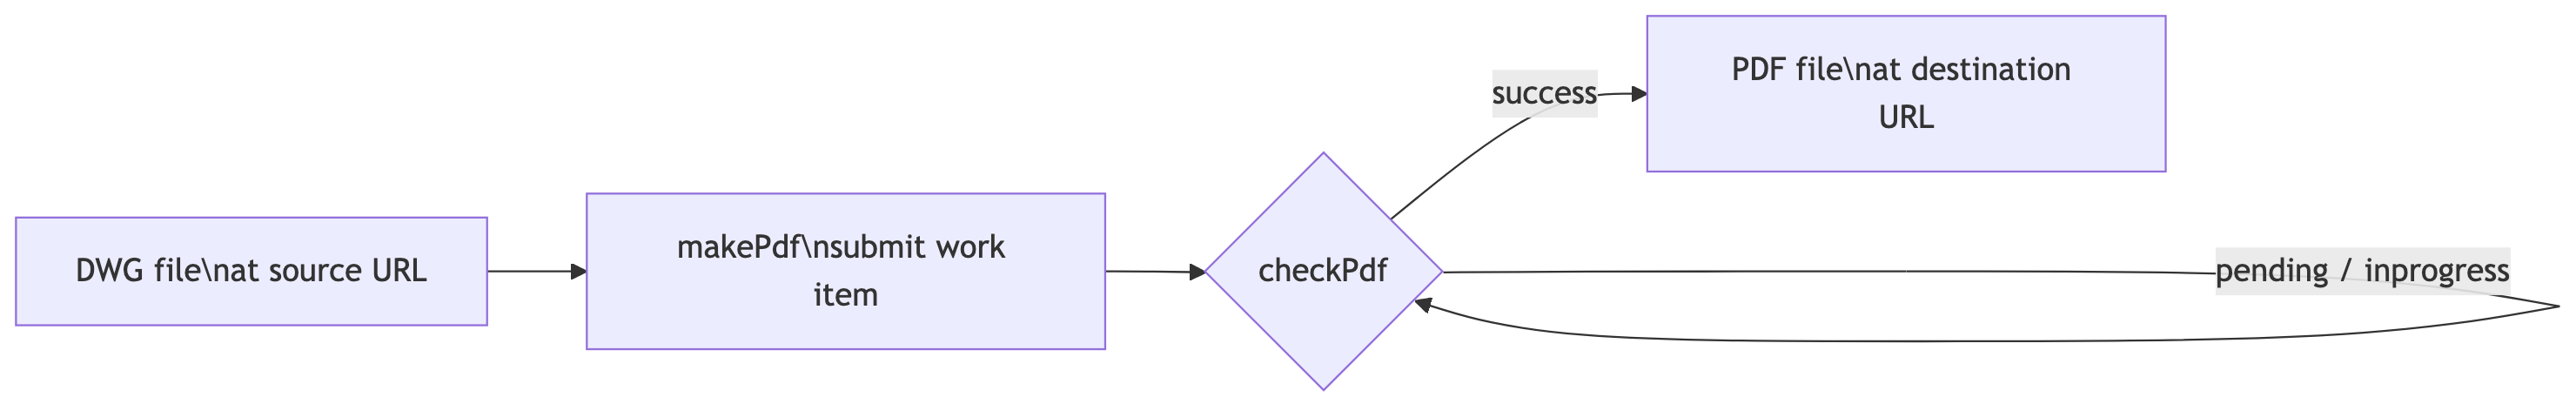
\includegraphics[width=13.46in,height=2.12in]{design-automation_files/figure-latex/mermaid-figure-1.png}

\section{Convert a DWG to PDF}\label{convert-a-dwg-to-pdf}

\texttt{makePdf()} submits the conversion job. The token needs the
\texttt{code:all} scope. This is specific to Design Automation and
different from the data scopes used elsewhere.

\begin{tcolorbox}[enhanced jigsaw, titlerule=0mm, colback=white, colframe=quarto-callout-warning-color-frame, bottomtitle=1mm, bottomrule=.15mm, coltitle=black, arc=.35mm, left=2mm, title=\textcolor{quarto-callout-warning-color}{\faExclamationTriangle}\hspace{0.5em}{Warning}, colbacktitle=quarto-callout-warning-color!10!white, toptitle=1mm, breakable, toprule=.15mm, rightrule=.15mm, leftrule=.75mm, opacitybacktitle=0.6, opacityback=0]

\textbf{Both \texttt{source} and \texttt{destination} must be publicly
accessible URLs.} Private Google Drive links, localhost paths, and
short-lived signed S3 URLs won't work. The AutoDesk cloud workers need
to be able to reach them directly. Use a public host or a pre-signed URL
with plenty of time left on it.

\end{tcolorbox}

\begin{Shaded}
\begin{Highlighting}[]
\NormalTok{resp }\OtherTok{\textless{}{-}} \FunctionTok{getToken}\NormalTok{(}
  \AttributeTok{id     =} \FunctionTok{Sys.getenv}\NormalTok{(}\StringTok{"client\_id"}\NormalTok{),}
  \AttributeTok{secret =} \FunctionTok{Sys.getenv}\NormalTok{(}\StringTok{"client\_secret"}\NormalTok{),}
  \AttributeTok{scope  =} \StringTok{"code:all"}
\NormalTok{)}
\NormalTok{myToken }\OtherTok{\textless{}{-}}\NormalTok{ resp}\SpecialCharTok{$}\NormalTok{content}\SpecialCharTok{$}\NormalTok{access\_token}
\end{Highlighting}
\end{Shaded}

\begin{Shaded}
\begin{Highlighting}[]
\NormalTok{mySource      }\OtherTok{\textless{}{-}} \StringTok{"http://download.autodesk.com/us/samplefiles/acad/visualization\_{-}\_aerial.dwg"}
\NormalTok{myDestination }\OtherTok{\textless{}{-}} \StringTok{"https://drive.google.com/folderview?id=0BygncDVHf60mTDZVNDltLThLNmM\&usp=sharing"}

\NormalTok{resp         }\OtherTok{\textless{}{-}} \FunctionTok{makePdf}\NormalTok{(}\AttributeTok{source =}\NormalTok{ mySource, }\AttributeTok{destination =}\NormalTok{ myDestination, }\AttributeTok{token =}\NormalTok{ myToken)}
\NormalTok{myWorkItemId }\OtherTok{\textless{}{-}}\NormalTok{ resp}\SpecialCharTok{$}\NormalTok{content}\SpecialCharTok{$}\NormalTok{id}
\NormalTok{resp}\SpecialCharTok{$}\NormalTok{content}
\CommentTok{\#\textgreater{} $id}
\CommentTok{\#\textgreater{} [1] "f47ac10b{-}58cc{-}4372{-}a567{-}0e02b2c3d479"}
\CommentTok{\#\textgreater{}}
\CommentTok{\#\textgreater{} $status}
\CommentTok{\#\textgreater{} [1] "pending"}
\CommentTok{\#\textgreater{}}
\CommentTok{\#\textgreater{} $stats$timeQueued}
\CommentTok{\#\textgreater{} [1] "2026{-}04{-}23T10:15:30.412Z"}
\end{Highlighting}
\end{Shaded}

\section{Poll for Completion}\label{poll-for-completion}

Use the work item \texttt{id} to check status. A simple DWG typically
takes \textbf{15--30 seconds}; complex drawings with many layers or
external references take longer.

\begin{Shaded}
\begin{Highlighting}[]
\ControlFlowTok{repeat}\NormalTok{ \{}
\NormalTok{  resp }\OtherTok{\textless{}{-}} \FunctionTok{checkPdf}\NormalTok{(}\AttributeTok{id =}\NormalTok{ myWorkItemId, }\AttributeTok{token =}\NormalTok{ myToken)}
  \FunctionTok{cat}\NormalTok{(}\StringTok{"Status:"}\NormalTok{, resp}\SpecialCharTok{$}\NormalTok{content}\SpecialCharTok{$}\NormalTok{status, }\StringTok{"}\SpecialCharTok{\textbackslash{}n}\StringTok{"}\NormalTok{)}
  \ControlFlowTok{if}\NormalTok{ (resp}\SpecialCharTok{$}\NormalTok{content}\SpecialCharTok{$}\NormalTok{status }\SpecialCharTok{==} \StringTok{"success"}\NormalTok{) }\ControlFlowTok{break}
  \FunctionTok{Sys.sleep}\NormalTok{(}\DecValTok{5}\NormalTok{)}
\NormalTok{\}}
\CommentTok{\#\textgreater{} Status: pending}
\CommentTok{\#\textgreater{} Status: inprogress}
\CommentTok{\#\textgreater{} Status: success}
\end{Highlighting}
\end{Shaded}

The full timing breakdown when it's done:

\begin{Shaded}
\begin{Highlighting}[]
\NormalTok{resp}\SpecialCharTok{$}\NormalTok{content}
\CommentTok{\#\textgreater{} $id}
\CommentTok{\#\textgreater{} [1] "f47ac10b{-}58cc{-}4372{-}a567{-}0e02b2c3d479"}
\CommentTok{\#\textgreater{}}
\CommentTok{\#\textgreater{} $status}
\CommentTok{\#\textgreater{} [1] "success"}
\CommentTok{\#\textgreater{}}
\CommentTok{\#\textgreater{} $stats$timeQueued}
\CommentTok{\#\textgreater{} [1] "2026{-}04{-}23T10:15:30.412Z"}
\CommentTok{\#\textgreater{}}
\CommentTok{\#\textgreater{} $stats$timeDownloadStarted}
\CommentTok{\#\textgreater{} [1] "2026{-}04{-}23T10:15:31.804Z"}
\CommentTok{\#\textgreater{}}
\CommentTok{\#\textgreater{} $stats$timeInstructionsStarted}
\CommentTok{\#\textgreater{} [1] "2026{-}04{-}23T10:15:34.217Z"}
\CommentTok{\#\textgreater{}}
\CommentTok{\#\textgreater{} $stats$timeFinished}
\CommentTok{\#\textgreater{} [1] "2026{-}04{-}23T10:15:48.993Z"}
\end{Highlighting}
\end{Shaded}

Once \texttt{status} is \texttt{"success"}, the PDF is waiting at your
\texttt{destination} URL.

\section{Batch Conversion}\label{batch-conversion}

Converting a folder of DWGs is just a loop:

\begin{Shaded}
\begin{Highlighting}[]
\NormalTok{dwg\_urls  }\OtherTok{\textless{}{-}} \FunctionTok{c}\NormalTok{(}
  \StringTok{"https://files.example.com/floor\_plan.dwg"}\NormalTok{,}
  \StringTok{"https://files.example.com/site\_plan.dwg"}\NormalTok{,}
  \StringTok{"https://files.example.com/elevations.dwg"}
\NormalTok{)}
\NormalTok{dest\_base }\OtherTok{\textless{}{-}} \StringTok{"https://output.example.com/pdfs/"}

\NormalTok{job\_ids }\OtherTok{\textless{}{-}} \FunctionTok{vapply}\NormalTok{(dwg\_urls, }\ControlFlowTok{function}\NormalTok{(url) \{}
\NormalTok{  fname }\OtherTok{\textless{}{-}} \FunctionTok{sub}\NormalTok{(}\StringTok{".*/"}\NormalTok{, }\StringTok{""}\NormalTok{, url)}
\NormalTok{  resp  }\OtherTok{\textless{}{-}} \FunctionTok{makePdf}\NormalTok{(}\AttributeTok{source      =}\NormalTok{ url,}
                   \AttributeTok{destination =} \FunctionTok{paste0}\NormalTok{(dest\_base, }\FunctionTok{sub}\NormalTok{(}\StringTok{"}\SpecialCharTok{\textbackslash{}\textbackslash{}}\StringTok{.dwg$"}\NormalTok{, }\StringTok{".pdf"}\NormalTok{, fname)),}
                   \AttributeTok{token       =}\NormalTok{ myToken)}
\NormalTok{  resp}\SpecialCharTok{$}\NormalTok{content}\SpecialCharTok{$}\NormalTok{id}
\NormalTok{\}, }\FunctionTok{character}\NormalTok{(}\DecValTok{1}\NormalTok{))}

\CommentTok{\# Poll until all jobs complete}
\ControlFlowTok{repeat}\NormalTok{ \{}
\NormalTok{  statuses }\OtherTok{\textless{}{-}} \FunctionTok{vapply}\NormalTok{(job\_ids, }\ControlFlowTok{function}\NormalTok{(id) \{}
    \FunctionTok{checkPdf}\NormalTok{(}\AttributeTok{id =}\NormalTok{ id, }\AttributeTok{token =}\NormalTok{ myToken)}\SpecialCharTok{$}\NormalTok{content}\SpecialCharTok{$}\NormalTok{status}
\NormalTok{  \}, }\FunctionTok{character}\NormalTok{(}\DecValTok{1}\NormalTok{))}
  \FunctionTok{cat}\NormalTok{(}\FunctionTok{format}\NormalTok{(}\FunctionTok{Sys.time}\NormalTok{(), }\StringTok{"\%H:\%M:\%S"}\NormalTok{), }\StringTok{"—"}\NormalTok{, }\FunctionTok{paste}\NormalTok{(statuses, }\AttributeTok{collapse =} \StringTok{" | "}\NormalTok{), }\StringTok{"}\SpecialCharTok{\textbackslash{}n}\StringTok{"}\NormalTok{)}
  \ControlFlowTok{if}\NormalTok{ (}\FunctionTok{all}\NormalTok{(statuses }\SpecialCharTok{==} \StringTok{"success"}\NormalTok{)) }\ControlFlowTok{break}
  \FunctionTok{Sys.sleep}\NormalTok{(}\DecValTok{10}\NormalTok{)}
\NormalTok{\}}
\CommentTok{\#\textgreater{} 10:20:05 — pending | pending | inprogress}
\CommentTok{\#\textgreater{} 10:20:15 — success | inprogress | inprogress}
\CommentTok{\#\textgreater{} 10:20:25 — success | success | success}
\end{Highlighting}
\end{Shaded}

\chapter{Reality Capture}\label{reality-capture}

Got a folder of overlapping photos and want a 3D mesh? That's the
Reality Capture API (also called Photo-to-3D). You upload the images,
AutoDesk's photogrammetry engine does the heavy lifting, and you
download a georeferenced 3D model --- no specialised hardware or
software required.

Common uses: - \textbf{As-built documentation} --- fly a drone over a
construction site each week and generate a mesh for each visit -
\textbf{Heritage recording} --- photograph a structure with a phone and
get a measurable 3D record - \textbf{Site topography} --- turn aerial
photos into a terrain mesh for civil design - \textbf{Mesh analysis} ---
feed the output into \texttt{Rvcg} via the \href{mesh-reading.qmd}{3D
Geometry} chapters

The full workflow goes like this:

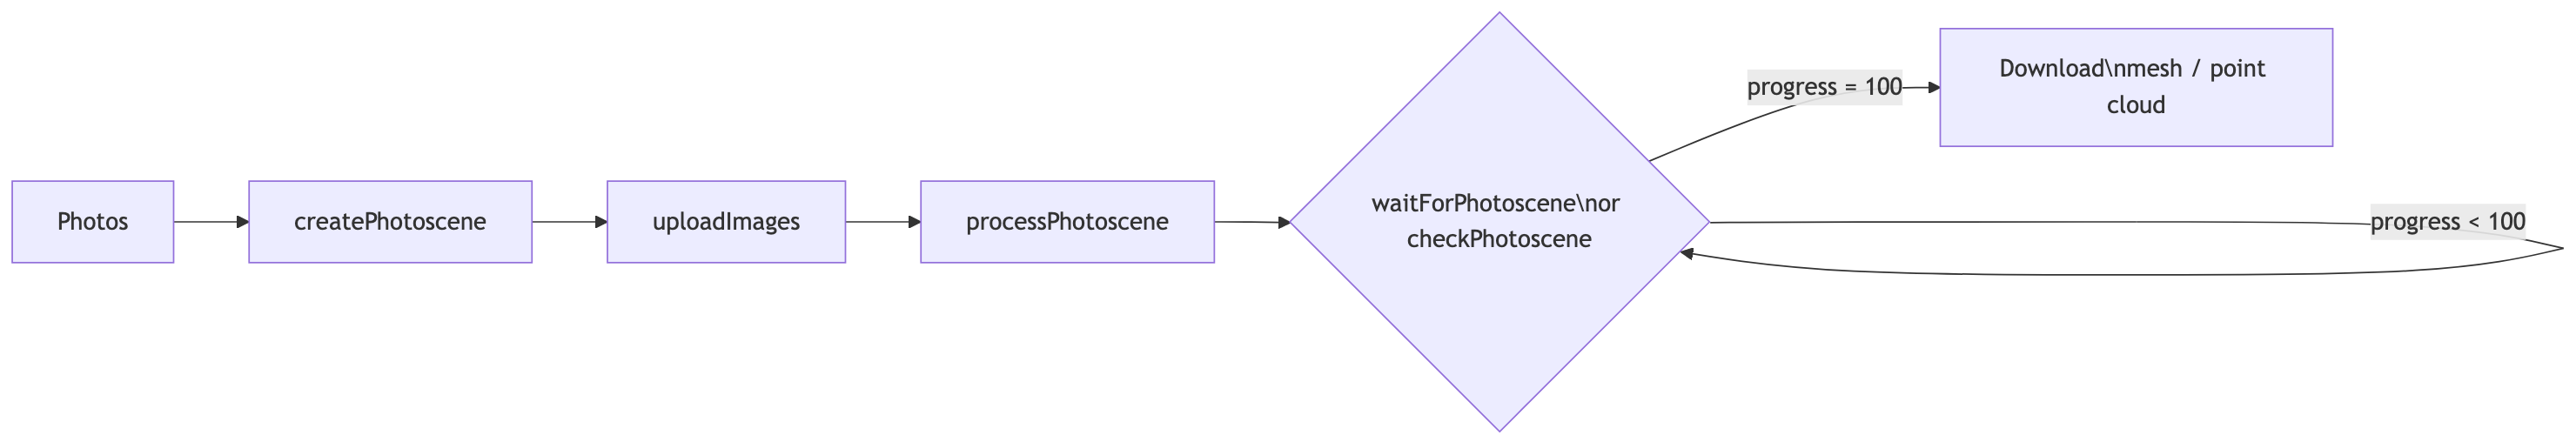
\includegraphics[width=17.77in,height=3.06in]{reality-capture_files/figure-latex/mermaid-figure-1.png}

\section{Before You Start}\label{before-you-start}

\begin{tcolorbox}[enhanced jigsaw, titlerule=0mm, colback=white, colframe=quarto-callout-tip-color-frame, bottomtitle=1mm, bottomrule=.15mm, coltitle=black, arc=.35mm, left=2mm, title=\textcolor{quarto-callout-tip-color}{\faLightbulb}\hspace{0.5em}{Tip}, colbacktitle=quarto-callout-tip-color!10!white, toptitle=1mm, breakable, toprule=.15mm, rightrule=.15mm, leftrule=.75mm, opacitybacktitle=0.6, opacityback=0]

\textbf{Good photos make good meshes.} A few guidelines that will save
you a lot of frustration:

\begin{itemize}
\tightlist
\item
  At least \textbf{20 images} per scene --- 50--200 is typical for a
  small structure
\item
  \textbf{60--80 \% overlap} between adjacent shots; every surface
  should appear in at least 3 photos
\item
  Consistent, diffuse lighting --- harsh shadows and mirror-like
  reflections confuse the algorithm
\item
  Move the camera \emph{around} the subject, don't just zoom in from one
  spot
\item
  GPS/EXIF tags are optional but improve georeferencing accuracy
\end{itemize}

\end{tcolorbox}

\section{Step 1: Authenticate}\label{step-1-authenticate}

Reality Capture needs \texttt{data:read} and \texttt{data:write} scopes:

\begin{Shaded}
\begin{Highlighting}[]
\FunctionTok{library}\NormalTok{(AutoDeskR)}

\NormalTok{resp    }\OtherTok{\textless{}{-}} \FunctionTok{getToken}\NormalTok{(}
  \AttributeTok{id     =} \FunctionTok{Sys.getenv}\NormalTok{(}\StringTok{"client\_id"}\NormalTok{),}
  \AttributeTok{secret =} \FunctionTok{Sys.getenv}\NormalTok{(}\StringTok{"client\_secret"}\NormalTok{),}
  \AttributeTok{scope  =} \StringTok{"data:read data:write"}
\NormalTok{)}
\NormalTok{myToken }\OtherTok{\textless{}{-}}\NormalTok{ resp}\SpecialCharTok{$}\NormalTok{content}\SpecialCharTok{$}\NormalTok{access\_token}
\end{Highlighting}
\end{Shaded}

\section{Step 2: Create a Photoscene}\label{step-2-create-a-photoscene}

A \textbf{photoscene} is the container for your images and output. The
\texttt{format} parameter controls what comes out the other end:

\begin{longtable}[]{@{}
  >{\raggedright\arraybackslash}p{(\linewidth - 2\tabcolsep) * \real{0.5000}}
  >{\raggedright\arraybackslash}p{(\linewidth - 2\tabcolsep) * \real{0.5000}}@{}}
\toprule\noalign{}
\begin{minipage}[b]{\linewidth}\raggedright
Format
\end{minipage} & \begin{minipage}[b]{\linewidth}\raggedright
Output
\end{minipage} \\
\midrule\noalign{}
\endhead
\bottomrule\noalign{}
\endlastfoot
\texttt{"rcm"} & AutoDesk ReCap project (default) \\
\texttt{"rcs"} & ReCap point cloud --- feeds into
\href{point-cloud-analysis.qmd}{Point Cloud Analysis} \\
\texttt{"obj"} & Wavefront OBJ mesh --- feeds into
\href{mesh-reading.qmd}{Reading OBJ and STL Meshes} \\
\texttt{"ortho"} & Orthophoto + DSM GeoTIFF \\
\texttt{"report"} & PDF quality report \\
\end{longtable}

\begin{Shaded}
\begin{Highlighting}[]
\NormalTok{ps             }\OtherTok{\textless{}{-}} \FunctionTok{createPhotoscene}\NormalTok{(}\AttributeTok{name =} \StringTok{"site{-}survey{-}2026"}\NormalTok{, }\AttributeTok{format =} \StringTok{"obj"}\NormalTok{, }\AttributeTok{token =}\NormalTok{ myToken)}
\NormalTok{myPhotosceneId }\OtherTok{\textless{}{-}}\NormalTok{ ps}\SpecialCharTok{$}\NormalTok{content}\SpecialCharTok{$}\NormalTok{photoscene}\SpecialCharTok{$}\NormalTok{photosceneid}
\NormalTok{myPhotosceneId}
\CommentTok{\#\textgreater{} [1] "K2RDAPFIN0OPKGU9B65Q2TJD"}
\end{Highlighting}
\end{Shaded}

\section{Step 3: Upload Images}\label{step-3-upload-images}

Pass a character vector of local file paths. AutoDeskR bundles them into
a single multipart POST. JPEG and PNG both work.

\begin{Shaded}
\begin{Highlighting}[]
\NormalTok{image\_files }\OtherTok{\textless{}{-}} \FunctionTok{list.files}\NormalTok{(}\StringTok{"photos/"}\NormalTok{, }\AttributeTok{pattern =} \StringTok{"}\SpecialCharTok{\textbackslash{}\textbackslash{}}\StringTok{.jpg$"}\NormalTok{, }\AttributeTok{full.names =} \ConstantTok{TRUE}\NormalTok{)}

\NormalTok{imgs }\OtherTok{\textless{}{-}} \FunctionTok{uploadImages}\NormalTok{(}
  \AttributeTok{photoscene\_id =}\NormalTok{ myPhotosceneId,}
  \AttributeTok{files         =}\NormalTok{ image\_files,}
  \AttributeTok{token         =}\NormalTok{ myToken}
\NormalTok{)}
\NormalTok{imgs}\SpecialCharTok{$}\NormalTok{content}\SpecialCharTok{$}\NormalTok{Files}\SpecialCharTok{$}\NormalTok{file[[}\DecValTok{1}\NormalTok{]]}
\CommentTok{\#\textgreater{} $filename}
\CommentTok{\#\textgreater{} [1] "site\_001.jpg"}
\CommentTok{\#\textgreater{}}
\CommentTok{\#\textgreater{} $fileid}
\CommentTok{\#\textgreater{} [1] "A1B2C3D4E5F6G7H8"}
\CommentTok{\#\textgreater{}}
\CommentTok{\#\textgreater{} $filesize}
\CommentTok{\#\textgreater{} [1] 4718592}
\end{Highlighting}
\end{Shaded}

\begin{tcolorbox}[enhanced jigsaw, titlerule=0mm, colback=white, colframe=quarto-callout-warning-color-frame, bottomtitle=1mm, bottomrule=.15mm, coltitle=black, arc=.35mm, left=2mm, title=\textcolor{quarto-callout-warning-color}{\faExclamationTriangle}\hspace{0.5em}{Warning}, colbacktitle=quarto-callout-warning-color!10!white, toptitle=1mm, breakable, toprule=.15mm, rightrule=.15mm, leftrule=.75mm, opacitybacktitle=0.6, opacityback=0]

\textbf{Free-tier limits:} Maximum \textbf{1,000 images per photoscene}
and \textbf{10 photoscenes per month}. Exceeding the quota returns a
\texttt{403\ Forbidden}. Upgrade to a paid plan for higher limits.

\end{tcolorbox}

\section{Step 4: Start Processing}\label{step-4-start-processing}

One call kicks off the reconstruction:

\begin{Shaded}
\begin{Highlighting}[]
\NormalTok{proc }\OtherTok{\textless{}{-}} \FunctionTok{processPhotoscene}\NormalTok{(}\AttributeTok{photoscene\_id =}\NormalTok{ myPhotosceneId, }\AttributeTok{token =}\NormalTok{ myToken)}
\NormalTok{proc}\SpecialCharTok{$}\NormalTok{content}\SpecialCharTok{$}\NormalTok{photoscene}\SpecialCharTok{$}\NormalTok{progressmsg}
\CommentTok{\#\textgreater{} [1] "Queued"}
\end{Highlighting}
\end{Shaded}

\section{Step 5: Wait for It}\label{step-5-wait-for-it}

\subsection{Option A --- Block until done
(recommended)}\label{option-a-block-until-done-recommended}

\texttt{waitForPhotoscene()} polls on a schedule and returns when the
job finishes. Set \texttt{verbose\ =\ TRUE} to watch the progress tick
up:

\begin{Shaded}
\begin{Highlighting}[]
\NormalTok{done }\OtherTok{\textless{}{-}} \FunctionTok{waitForPhotoscene}\NormalTok{(}
  \AttributeTok{photoscene\_id =}\NormalTok{ myPhotosceneId,}
  \AttributeTok{token         =}\NormalTok{ myToken,}
  \AttributeTok{interval      =} \DecValTok{60}\NormalTok{,    }\CommentTok{\# check every 60 seconds}
  \AttributeTok{timeout       =} \DecValTok{3600}\NormalTok{,  }\CommentTok{\# give up after an hour}
  \AttributeTok{verbose       =} \ConstantTok{TRUE}
\NormalTok{)}
\CommentTok{\#\textgreater{} Reality Capture progress: 0 {-} Queued}
\CommentTok{\#\textgreater{} Reality Capture progress: 10 {-} Uploading files}
\CommentTok{\#\textgreater{} Reality Capture progress: 35 {-} Calibrating cameras}
\CommentTok{\#\textgreater{} Reality Capture progress: 60 {-} Building point cloud}
\CommentTok{\#\textgreater{} Reality Capture progress: 85 {-} Generating mesh}
\CommentTok{\#\textgreater{} Reality Capture progress: 100 {-} Done}
\end{Highlighting}
\end{Shaded}

\subsection{Option B --- Manual polling}\label{option-b-manual-polling}

If you want more control, call \texttt{checkPhotoscene()} yourself:

\begin{Shaded}
\begin{Highlighting}[]
\NormalTok{status }\OtherTok{\textless{}{-}} \FunctionTok{checkPhotoscene}\NormalTok{(}\AttributeTok{photoscene\_id =}\NormalTok{ myPhotosceneId, }\AttributeTok{token =}\NormalTok{ myToken)}
\NormalTok{status}\SpecialCharTok{$}\NormalTok{content}\SpecialCharTok{$}\NormalTok{photoscene}\SpecialCharTok{$}\NormalTok{progress}
\CommentTok{\#\textgreater{} [1] "75"}
\NormalTok{status}\SpecialCharTok{$}\NormalTok{content}\SpecialCharTok{$}\NormalTok{photoscene}\SpecialCharTok{$}\NormalTok{progressmsg}
\CommentTok{\#\textgreater{} [1] "Processing geometry"}
\end{Highlighting}
\end{Shaded}

\begin{tcolorbox}[enhanced jigsaw, titlerule=0mm, colback=white, colframe=quarto-callout-warning-color-frame, bottomtitle=1mm, bottomrule=.15mm, coltitle=black, arc=.35mm, left=2mm, title=\textcolor{quarto-callout-warning-color}{\faExclamationTriangle}\hspace{0.5em}{Warning}, colbacktitle=quarto-callout-warning-color!10!white, toptitle=1mm, breakable, toprule=.15mm, rightrule=.15mm, leftrule=.75mm, opacitybacktitle=0.6, opacityback=0]

\textbf{Processing time scales with image count.} A 50-image scene
typically takes 5--15 minutes; 500 images may take over an hour. Set
\texttt{timeout} generously --- there's nothing worse than a premature
timeout on an 80-minute job.

\end{tcolorbox}

\section{Step 6: Download the Output}\label{step-6-download-the-output}

When \texttt{progress} hits \texttt{"100"}, retrieve the download URL
and save the mesh locally:

\begin{Shaded}
\begin{Highlighting}[]
\NormalTok{output\_url }\OtherTok{\textless{}{-}}\NormalTok{ done}\SpecialCharTok{$}\NormalTok{content}\SpecialCharTok{$}\NormalTok{photoscene}\SpecialCharTok{$}\NormalTok{scenelink}

\FunctionTok{download.file}\NormalTok{(}
  \AttributeTok{url      =} \FunctionTok{paste0}\NormalTok{(output\_url, }\StringTok{"/output.obj"}\NormalTok{),}
  \AttributeTok{destfile =} \StringTok{"site{-}survey{-}2026.obj"}\NormalTok{,}
  \AttributeTok{headers  =} \FunctionTok{c}\NormalTok{(}\AttributeTok{Authorization =} \FunctionTok{paste}\NormalTok{(}\StringTok{"Bearer"}\NormalTok{, myToken))}
\NormalTok{)}
\end{Highlighting}
\end{Shaded}

From here, the OBJ file is ready for \href{mesh-reading.qmd}{Reading OBJ
and STL Meshes} or further translation via the
\hyperref[model-derivative]{Model Derivative} API.

\chapter{Viewer}\label{viewer}

The AutoDesk Viewer is a WebGL-based 3D model browser that runs entirely
in the browser. With AutoDeskR, you can embed it in a Shiny app with a
single function call --- no JavaScript required. Rotate, zoom, and
inspect your models without leaving R.

Before launching the viewer, you need a file translated to SVF format
and its encoded URN --- the \hyperref[model-derivative]{Model
Derivative} chapter covers both steps.

\section{Launch the Viewer}\label{launch-the-viewer}

\texttt{viewer3D()} opens a Shiny app with the viewer pre-loaded. The
\texttt{viewerType} parameter controls the UI chrome:

\begin{longtable}[]{@{}
  >{\raggedright\arraybackslash}p{(\linewidth - 2\tabcolsep) * \real{0.1972}}
  >{\raggedright\arraybackslash}p{(\linewidth - 2\tabcolsep) * \real{0.8028}}@{}}
\toprule\noalign{}
\begin{minipage}[b]{\linewidth}\raggedright
\texttt{viewerType}
\end{minipage} & \begin{minipage}[b]{\linewidth}\raggedright
What you get
\end{minipage} \\
\midrule\noalign{}
\endhead
\bottomrule\noalign{}
\endlastfoot
\texttt{"header"} & Full toolbar, navigation panels, and settings
(default) \\
\texttt{"headless"} & Viewer canvas only --- clean embed for
dashboards \\
\texttt{"vr"} & WebVR mode, optimised for mobile \\
\end{longtable}

\begin{Shaded}
\begin{Highlighting}[]
\NormalTok{resp }\OtherTok{\textless{}{-}} \FunctionTok{getToken}\NormalTok{(}
  \AttributeTok{id     =} \FunctionTok{Sys.getenv}\NormalTok{(}\StringTok{"client\_id"}\NormalTok{),}
  \AttributeTok{secret =} \FunctionTok{Sys.getenv}\NormalTok{(}\StringTok{"client\_secret"}\NormalTok{),}
  \AttributeTok{scope  =} \StringTok{"data:read"}
\NormalTok{)}
\NormalTok{myToken      }\OtherTok{\textless{}{-}}\NormalTok{ resp}\SpecialCharTok{$}\NormalTok{content}\SpecialCharTok{$}\NormalTok{access\_token}
\NormalTok{myEncodedUrn }\OtherTok{\textless{}{-}}\NormalTok{ jsonlite}\SpecialCharTok{::}\FunctionTok{base64\_enc}\NormalTok{(}\FunctionTok{Sys.getenv}\NormalTok{(}\StringTok{"urn"}\NormalTok{))}

\CommentTok{\# Full viewer — great for exploration}
\FunctionTok{viewer3D}\NormalTok{(}\AttributeTok{urn =}\NormalTok{ myEncodedUrn, }\AttributeTok{token =}\NormalTok{ myToken)}

\CommentTok{\# Headless — embed in a dashboard without the toolbar chrome}
\FunctionTok{viewer3D}\NormalTok{(}\AttributeTok{urn =}\NormalTok{ myEncodedUrn, }\AttributeTok{token =}\NormalTok{ myToken, }\AttributeTok{viewerType =} \StringTok{"headless"}\NormalTok{)}

\CommentTok{\# VR mode for a phone or headset}
\FunctionTok{viewer3D}\NormalTok{(}\AttributeTok{urn =}\NormalTok{ myEncodedUrn, }\AttributeTok{token =}\NormalTok{ myToken, }\AttributeTok{viewerType =} \StringTok{"vr"}\NormalTok{)}
\end{Highlighting}
\end{Shaded}

\section{Embed in a Shiny App}\label{embed-in-a-shiny-app}

\texttt{viewerUI()} drops the viewer into any Shiny layout as a module.
The \texttt{id} parameter namespaces the module so multiple viewers can
live on the same page without stepping on each other.

\begin{Shaded}
\begin{Highlighting}[]
\FunctionTok{library}\NormalTok{(shiny)}
\FunctionTok{library}\NormalTok{(AutoDeskR)}

\NormalTok{ui }\OtherTok{\textless{}{-}} \FunctionTok{fluidPage}\NormalTok{(}
  \FunctionTok{viewerUI}\NormalTok{(}\StringTok{"viewer1"}\NormalTok{, }\AttributeTok{urn =}\NormalTok{ myEncodedUrn, }\AttributeTok{token =}\NormalTok{ myToken)}
\NormalTok{)}

\NormalTok{server }\OtherTok{\textless{}{-}} \ControlFlowTok{function}\NormalTok{(input, output, session) \{\}}

\FunctionTok{shinyApp}\NormalTok{(ui, server)}
\end{Highlighting}
\end{Shaded}

\subsection{Viewer in a Tab Panel}\label{viewer-in-a-tab-panel}

Headless mode is perfect for a multi-tab layout --- the viewer sits in
one tab and data tables or charts in another:

\begin{Shaded}
\begin{Highlighting}[]
\NormalTok{ui }\OtherTok{\textless{}{-}} \FunctionTok{fluidPage}\NormalTok{(}
  \FunctionTok{tabsetPanel}\NormalTok{(}
    \FunctionTok{tabPanel}\NormalTok{(}\StringTok{"Model"}\NormalTok{,}
      \FunctionTok{viewerUI}\NormalTok{(}\StringTok{"viewer1"}\NormalTok{, myEncodedUrn, myToken, }\AttributeTok{viewerType =} \StringTok{"headless"}\NormalTok{)}
\NormalTok{    ),}
    \FunctionTok{tabPanel}\NormalTok{(}\StringTok{"Metadata"}\NormalTok{,}
      \FunctionTok{verbatimTextOutput}\NormalTok{(}\StringTok{"meta"}\NormalTok{)}
\NormalTok{    ),}
    \FunctionTok{tabPanel}\NormalTok{(}\StringTok{"Layer Chart"}\NormalTok{,}
      \FunctionTok{plotOutput}\NormalTok{(}\StringTok{"layer\_plot"}\NormalTok{)}
\NormalTok{    )}
\NormalTok{  )}
\NormalTok{)}

\NormalTok{server }\OtherTok{\textless{}{-}} \ControlFlowTok{function}\NormalTok{(input, output, session) \{}
\NormalTok{  output}\SpecialCharTok{$}\NormalTok{meta }\OtherTok{\textless{}{-}} \FunctionTok{renderPrint}\NormalTok{(\{}
    \CommentTok{\# getData() results displayed alongside the viewer}
\NormalTok{  \})}
\NormalTok{\}}

\FunctionTok{shinyApp}\NormalTok{(ui, server)}
\end{Highlighting}
\end{Shaded}

\subsection{Viewer + Sensor Dashboard}\label{viewer-sensor-dashboard}

Pair the headless viewer with a \texttt{dygraphs} time-series panel for
a live digital twin layout --- see the \href{live-dashboards.qmd}{Live
Dashboards} chapter for the full implementation:

\begin{Shaded}
\begin{Highlighting}[]
\FunctionTok{library}\NormalTok{(dygraphs)}

\NormalTok{ui }\OtherTok{\textless{}{-}} \FunctionTok{fluidPage}\NormalTok{(}
  \FunctionTok{fluidRow}\NormalTok{(}
    \FunctionTok{column}\NormalTok{(}\DecValTok{7}\NormalTok{, }\FunctionTok{viewerUI}\NormalTok{(}\StringTok{"twin\_viewer"}\NormalTok{, myEncodedUrn, myToken, }\AttributeTok{viewerType =} \StringTok{"headless"}\NormalTok{)),}
    \FunctionTok{column}\NormalTok{(}\DecValTok{5}\NormalTok{, }\FunctionTok{dygraphOutput}\NormalTok{(}\StringTok{"sensor\_plot"}\NormalTok{, }\AttributeTok{height =} \StringTok{"500px"}\NormalTok{))}
\NormalTok{  )}
\NormalTok{)}
\end{Highlighting}
\end{Shaded}

\section{What's Displayed}\label{whats-displayed}

The viewer renders whatever the SVF translation produced. For a DWG
file, that's the full drawing geometry organised by layer. For a Revit
file, it's the full BIM model with element properties accessible in the
side panel. Click any element in the viewer to inspect its properties
--- the same data that \texttt{getData()} returns programmatically.

\part{3D Geometry \& Meshes}

\chapter{Reading OBJ and STL Meshes}\label{reading-obj-and-stl-meshes}

Once you've translated a CAD file through the
\hyperref[model-derivative]{Model Derivative} API, you've got an OBJ or
STL file sitting on disk. Now the fun part: loading it into R.

\texttt{rgl} (Adler, Murdoch, et al. 2024) and \texttt{Rvcg} (Schlager
2024) both read OBJ and STL files. \texttt{rgl} is great for interactive
viewing; \texttt{Rvcg} is the one to reach for when you want to compute
things. It returns a \texttt{tmesh3d} object that plays nicely with the
whole \texttt{Rvcg} family of analysis functions.

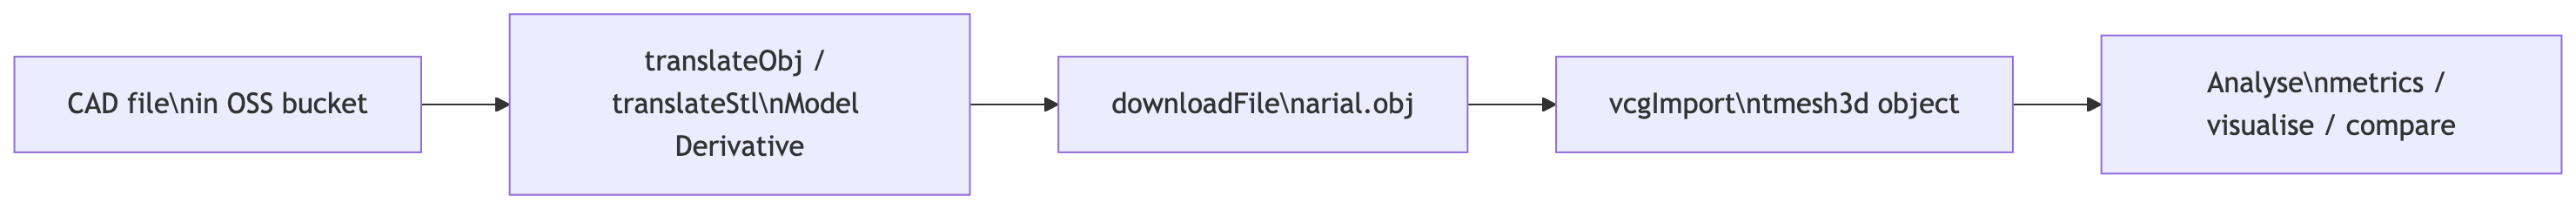
\includegraphics[width=15.16in,height=1.23in]{mesh-reading_files/figure-latex/mermaid-figure-1.png}

\section{Prerequisites}\label{prerequisites-1}

\begin{Shaded}
\begin{Highlighting}[]
\FunctionTok{install.packages}\NormalTok{(}\FunctionTok{c}\NormalTok{(}\StringTok{"rgl"}\NormalTok{, }\StringTok{"Rvcg"}\NormalTok{))}
\end{Highlighting}
\end{Shaded}

\section{Getting the OBJ File}\label{getting-the-obj-file}

The full upstream chain, translate, poll, get output URN, download,
picks up where the \hyperref[model-derivative]{Model Derivative} chapter
left off:

\begin{Shaded}
\begin{Highlighting}[]
\FunctionTok{library}\NormalTok{(AutoDeskR)}

\NormalTok{resp     }\OtherTok{\textless{}{-}} \FunctionTok{getToken}\NormalTok{(}\AttributeTok{id     =} \FunctionTok{Sys.getenv}\NormalTok{(}\StringTok{"client\_id"}\NormalTok{),}
                     \AttributeTok{secret =} \FunctionTok{Sys.getenv}\NormalTok{(}\StringTok{"client\_secret"}\NormalTok{),}
                     \AttributeTok{scope  =} \StringTok{"data:read data:write"}\NormalTok{)}
\NormalTok{myToken  }\OtherTok{\textless{}{-}}\NormalTok{ resp}\SpecialCharTok{$}\NormalTok{content}\SpecialCharTok{$}\NormalTok{access\_token}

\NormalTok{myEncodedUrn }\OtherTok{\textless{}{-}}\NormalTok{ jsonlite}\SpecialCharTok{::}\FunctionTok{base64\_enc}\NormalTok{(}\FunctionTok{Sys.getenv}\NormalTok{(}\StringTok{"urn"}\NormalTok{))}

\FunctionTok{translateObj}\NormalTok{(}\AttributeTok{urn =}\NormalTok{ myEncodedUrn, }\AttributeTok{token =}\NormalTok{ myToken)}

\ControlFlowTok{repeat}\NormalTok{ \{}
\NormalTok{  status }\OtherTok{\textless{}{-}} \FunctionTok{checkFile}\NormalTok{(}\AttributeTok{urn =}\NormalTok{ myEncodedUrn, }\AttributeTok{token =}\NormalTok{ myToken)}
  \ControlFlowTok{if}\NormalTok{ (status}\SpecialCharTok{$}\NormalTok{content}\SpecialCharTok{$}\NormalTok{status }\SpecialCharTok{==} \StringTok{"success"}\NormalTok{) }\ControlFlowTok{break}
  \FunctionTok{Sys.sleep}\NormalTok{(}\DecValTok{5}\NormalTok{)}
\NormalTok{\}}

\NormalTok{outputUrn       }\OtherTok{\textless{}{-}} \FunctionTok{getOutputUrn}\NormalTok{(}\AttributeTok{urn =}\NormalTok{ myEncodedUrn, }\AttributeTok{token =}\NormalTok{ myToken)}
\NormalTok{myOutputUrn     }\OtherTok{\textless{}{-}}\NormalTok{ outputUrn}\SpecialCharTok{$}\NormalTok{content}\SpecialCharTok{$}\NormalTok{derivatives[[}\DecValTok{1}\NormalTok{]]}\SpecialCharTok{$}\NormalTok{children[[}\DecValTok{1}\NormalTok{]]}\SpecialCharTok{$}\NormalTok{urn}
\NormalTok{myEncodedOutput }\OtherTok{\textless{}{-}}\NormalTok{ jsonlite}\SpecialCharTok{::}\FunctionTok{base64\_enc}\NormalTok{(myOutputUrn)}

\FunctionTok{downloadFile}\NormalTok{(}\AttributeTok{urn        =}\NormalTok{ myEncodedUrn,}
             \AttributeTok{output\_urn =}\NormalTok{ myEncodedOutput,}
             \AttributeTok{token      =}\NormalTok{ myToken,}
             \AttributeTok{destfile   =} \StringTok{"aerial.obj"}\NormalTok{)}
\end{Highlighting}
\end{Shaded}

\section{Reading with Rvcg (recommended for
analysis)}\label{reading-with-rvcg-recommended-for-analysis}

\texttt{vcgImport()} parses the OBJ and returns a \texttt{tmesh3d}, a
list with a vertex matrix (\texttt{vb}) and a triangle index matrix
(\texttt{it}). Every analysis function in the next three chapters works
on this object.

\begin{Shaded}
\begin{Highlighting}[]
\FunctionTok{library}\NormalTok{(Rvcg)}
\NormalTok{mesh\_vcg }\OtherTok{\textless{}{-}} \FunctionTok{vcgImport}\NormalTok{(}\StringTok{"aerial.obj"}\NormalTok{)}
\FunctionTok{str}\NormalTok{(mesh\_vcg)}
\CommentTok{\#\textgreater{} List of 4}
\CommentTok{\#\textgreater{}  $ vb     : num [1:4, 1:2847] ...   \# homogeneous vertex coords (X/Y/Z/W)}
\CommentTok{\#\textgreater{}  $ it     : int [1:3, 1:1832] ...   \# triangle face indices}
\CommentTok{\#\textgreater{}  $ normals: num [1:4, 1:2847] ...}
\CommentTok{\#\textgreater{}  $ material: list()}
\end{Highlighting}
\end{Shaded}

\section{Reading with rgl (for interactive
viewing)}\label{reading-with-rgl-for-interactive-viewing}

\texttt{readOBJ()} returns a similar \texttt{mesh3d} object that you can
render immediately:

\begin{Shaded}
\begin{Highlighting}[]
\FunctionTok{library}\NormalTok{(rgl)}
\NormalTok{mesh\_obj }\OtherTok{\textless{}{-}} \FunctionTok{readOBJ}\NormalTok{(}\StringTok{"aerial.obj"}\NormalTok{)}
\end{Highlighting}
\end{Shaded}

\begin{tcolorbox}[enhanced jigsaw, titlerule=0mm, colback=white, colframe=quarto-callout-tip-color-frame, bottomtitle=1mm, bottomrule=.15mm, coltitle=black, arc=.35mm, left=2mm, title=\textcolor{quarto-callout-tip-color}{\faLightbulb}\hspace{0.5em}{Tip}, colbacktitle=quarto-callout-tip-color!10!white, toptitle=1mm, breakable, toprule=.15mm, rightrule=.15mm, leftrule=.75mm, opacitybacktitle=0.6, opacityback=0]

OBJ files from the Model Derivative API sometimes contain multiple named
objects (one per CAD layer or body). \texttt{vcgImport()} merges them
into a single mesh by default. Use
\texttt{rgl::readOBJ(material\ =\ TRUE)} if you need to keep them
separate for per-layer analysis.

\end{tcolorbox}

\section{Reading STL}\label{reading-stl}

Exactly the same call works for STL files. \texttt{vcgImport()} handles
both formats transparently:

\begin{Shaded}
\begin{Highlighting}[]
\NormalTok{mesh\_stl }\OtherTok{\textless{}{-}} \FunctionTok{vcgImport}\NormalTok{(}\StringTok{"aerial.stl"}\NormalTok{)}
\CommentTok{\# Same tmesh3d structure — all subsequent chapters work identically on OBJ and STL}
\end{Highlighting}
\end{Shaded}

\section{Quick Inspection}\label{quick-inspection}

A few fast checks to make sure the mesh loaded correctly:

\begin{Shaded}
\begin{Highlighting}[]
\FunctionTok{cat}\NormalTok{(}\StringTok{"Vertices:"}\NormalTok{, }\FunctionTok{ncol}\NormalTok{(mesh\_vcg}\SpecialCharTok{$}\NormalTok{vb), }\StringTok{"}\SpecialCharTok{\textbackslash{}n}\StringTok{"}\NormalTok{)}
\CommentTok{\#\textgreater{} Vertices: 2847}
\FunctionTok{cat}\NormalTok{(}\StringTok{"Faces:   "}\NormalTok{, }\FunctionTok{ncol}\NormalTok{(mesh\_vcg}\SpecialCharTok{$}\NormalTok{it), }\StringTok{"}\SpecialCharTok{\textbackslash{}n}\StringTok{"}\NormalTok{)}
\CommentTok{\#\textgreater{} Faces:    1832}

\CommentTok{\# Coordinate ranges — useful sanity check that units are what you expect}
\FunctionTok{apply}\NormalTok{(}\FunctionTok{t}\NormalTok{(mesh\_vcg}\SpecialCharTok{$}\NormalTok{vb[}\DecValTok{1}\SpecialCharTok{:}\DecValTok{3}\NormalTok{, ]), }\DecValTok{2}\NormalTok{, range)}
\CommentTok{\#\textgreater{}           [,1]      [,2]  [,3]}
\CommentTok{\#\textgreater{} [1,] {-}142.830  {-}98.470  0.000}
\CommentTok{\#\textgreater{} [2,]  318.620  241.190 12.500}
\end{Highlighting}
\end{Shaded}

The \texttt{mesh\_vcg} object lives on from here through the
\href{mesh-metrics.qmd}{Mesh Metrics}, \href{mesh-visualisation.qmd}{3D
Visualisation}, and \href{mesh-comparison.qmd}{Mesh Comparison}
chapters, so keep it in your environment.

\chapter{Mesh Metrics}\label{mesh-metrics}

Got a mesh? Let's measure it. \texttt{Rvcg} (Schlager 2024) and
\texttt{geometry} (Roussel, Sterratt, et al. 2024) turn a
\texttt{tmesh3d} into a full geometric report, surface area, volume,
bounding box, centroid. These numbers are useful for QA (does the
translated geometry match the design intent?), quantity takeoff, and as
inputs to dashboards and reports.

This chapter uses \texttt{mesh\_vcg} from
\hyperref[reading-obj-and-stl-meshes]{Reading OBJ and STL Meshes}.

\section{Surface Area}\label{surface-area}

\begin{Shaded}
\begin{Highlighting}[]
\FunctionTok{library}\NormalTok{(Rvcg)}
\NormalTok{area }\OtherTok{\textless{}{-}} \FunctionTok{vcgArea}\NormalTok{(mesh\_vcg)}
\NormalTok{area}
\CommentTok{\#\textgreater{} [1] 14823.6   \# square units — same as the DWG drawing units}
\end{Highlighting}
\end{Shaded}

\section{Volume}\label{volume}

\begin{Shaded}
\begin{Highlighting}[]
\NormalTok{vol }\OtherTok{\textless{}{-}} \FunctionTok{vcgVolume}\NormalTok{(mesh\_vcg)}
\NormalTok{vol}
\CommentTok{\#\textgreater{} [1] 48219.3}
\end{Highlighting}
\end{Shaded}

\begin{tcolorbox}[enhanced jigsaw, titlerule=0mm, colback=white, colframe=quarto-callout-warning-color-frame, bottomtitle=1mm, bottomrule=.15mm, coltitle=black, arc=.35mm, left=2mm, title=\textcolor{quarto-callout-warning-color}{\faExclamationTriangle}\hspace{0.5em}{Warning}, colbacktitle=quarto-callout-warning-color!10!white, toptitle=1mm, breakable, toprule=.15mm, rightrule=.15mm, leftrule=.75mm, opacitybacktitle=0.6, opacityback=0]

\texttt{vcgVolume()} only gives meaningful results for
\textbf{watertight (closed) meshes}. OBJ files translated from open 2D
DWG drawings are almost never watertight, so this number will be
unreliable. Use the convex hull fallback below instead.

\end{tcolorbox}

\section{Bounding Box}\label{bounding-box}

\begin{Shaded}
\begin{Highlighting}[]
\NormalTok{bb }\OtherTok{\textless{}{-}} \FunctionTok{apply}\NormalTok{(}\FunctionTok{t}\NormalTok{(mesh\_vcg}\SpecialCharTok{$}\NormalTok{vb[}\DecValTok{1}\SpecialCharTok{:}\DecValTok{3}\NormalTok{, ]), }\DecValTok{2}\NormalTok{, range)}
\FunctionTok{rownames}\NormalTok{(bb) }\OtherTok{\textless{}{-}} \FunctionTok{c}\NormalTok{(}\StringTok{"min"}\NormalTok{, }\StringTok{"max"}\NormalTok{)}
\FunctionTok{colnames}\NormalTok{(bb) }\OtherTok{\textless{}{-}} \FunctionTok{c}\NormalTok{(}\StringTok{"X"}\NormalTok{, }\StringTok{"Y"}\NormalTok{, }\StringTok{"Z"}\NormalTok{)}
\NormalTok{bb}
\CommentTok{\#\textgreater{}        X        Y      Z}
\CommentTok{\#\textgreater{} min {-}142.83  {-}98.47   0.00}
\CommentTok{\#\textgreater{} max  318.62  241.19  12.50}

\FunctionTok{diff}\NormalTok{(bb)   }\CommentTok{\# width / depth / height}
\CommentTok{\#\textgreater{}       X      Y     Z}
\CommentTok{\#\textgreater{} 461.45 339.66 12.50}
\end{Highlighting}
\end{Shaded}

\section{Centroid}\label{centroid}

\begin{Shaded}
\begin{Highlighting}[]
\NormalTok{centroid }\OtherTok{\textless{}{-}} \FunctionTok{colMeans}\NormalTok{(}\FunctionTok{t}\NormalTok{(mesh\_vcg}\SpecialCharTok{$}\NormalTok{vb[}\DecValTok{1}\SpecialCharTok{:}\DecValTok{3}\NormalTok{, ]))}
\FunctionTok{names}\NormalTok{(centroid) }\OtherTok{\textless{}{-}} \FunctionTok{c}\NormalTok{(}\StringTok{"X"}\NormalTok{, }\StringTok{"Y"}\NormalTok{, }\StringTok{"Z"}\NormalTok{)}
\NormalTok{centroid}
\CommentTok{\#\textgreater{}      X      Y     Z}
\CommentTok{\#\textgreater{}  87.90  71.36   6.25}
\end{Highlighting}
\end{Shaded}

\section{Convex Hull Volume}\label{convex-hull-volume}

For open (non-watertight) meshes, \texttt{geometry::convhulln()}
(Roussel, Sterratt, et al. 2024) computes the volume and surface area of
the convex hull, a conservative upper bound that doesn't require a
closed surface:

\begin{Shaded}
\begin{Highlighting}[]
\FunctionTok{library}\NormalTok{(geometry)}
\NormalTok{pts  }\OtherTok{\textless{}{-}} \FunctionTok{t}\NormalTok{(mesh\_vcg}\SpecialCharTok{$}\NormalTok{vb[}\DecValTok{1}\SpecialCharTok{:}\DecValTok{3}\NormalTok{, ])}
\NormalTok{hull }\OtherTok{\textless{}{-}} \FunctionTok{convhulln}\NormalTok{(pts, }\AttributeTok{options =} \StringTok{"FA"}\NormalTok{)}
\NormalTok{hull}\SpecialCharTok{$}\NormalTok{vol}
\CommentTok{\#\textgreater{} [1] 1871423.5}
\NormalTok{hull}\SpecialCharTok{$}\NormalTok{area}
\CommentTok{\#\textgreater{} [1] 216834.2}
\end{Highlighting}
\end{Shaded}

\section{Summary Table}\label{summary-table}

Pull all the numbers together into a single data frame, ready to feed
into a \texttt{gt} table or write to CSV:

\begin{Shaded}
\begin{Highlighting}[]
\NormalTok{mesh\_summary }\OtherTok{\textless{}{-}} \FunctionTok{data.frame}\NormalTok{(}
  \AttributeTok{metric =} \FunctionTok{c}\NormalTok{(}\StringTok{"Vertices"}\NormalTok{, }\StringTok{"Faces"}\NormalTok{, }\StringTok{"Surface area"}\NormalTok{,}
             \StringTok{"Convex hull volume"}\NormalTok{, }\StringTok{"Convex hull area"}\NormalTok{,}
             \StringTok{"Bounding box X"}\NormalTok{, }\StringTok{"Bounding box Y"}\NormalTok{, }\StringTok{"Bounding box Z"}\NormalTok{,}
             \StringTok{"Centroid X"}\NormalTok{, }\StringTok{"Centroid Y"}\NormalTok{, }\StringTok{"Centroid Z"}\NormalTok{),}
  \AttributeTok{value  =} \FunctionTok{c}\NormalTok{(}\FunctionTok{ncol}\NormalTok{(mesh\_vcg}\SpecialCharTok{$}\NormalTok{vb), }\FunctionTok{ncol}\NormalTok{(mesh\_vcg}\SpecialCharTok{$}\NormalTok{it), area,}
\NormalTok{             hull}\SpecialCharTok{$}\NormalTok{vol, hull}\SpecialCharTok{$}\NormalTok{area,}
             \FunctionTok{diff}\NormalTok{(bb)[}\DecValTok{1}\NormalTok{], }\FunctionTok{diff}\NormalTok{(bb)[}\DecValTok{2}\NormalTok{], }\FunctionTok{diff}\NormalTok{(bb)[}\DecValTok{3}\NormalTok{],}
\NormalTok{             centroid[}\DecValTok{1}\NormalTok{], centroid[}\DecValTok{2}\NormalTok{], centroid[}\DecValTok{3}\NormalTok{])}
\NormalTok{)}
\NormalTok{mesh\_summary}
\CommentTok{\#\textgreater{}                metric        value}
\CommentTok{\#\textgreater{} 1            Vertices     2847.000}
\CommentTok{\#\textgreater{} 2               Faces     1832.000}
\CommentTok{\#\textgreater{} 3        Surface area    14823.600}
\CommentTok{\#\textgreater{} 4  Convex hull volume  1871423.500}
\CommentTok{\#\textgreater{} 5    Convex hull area   216834.200}
\CommentTok{\#\textgreater{} 6      Bounding box X      461.450}
\CommentTok{\#\textgreater{} 7      Bounding box Y      339.660}
\CommentTok{\#\textgreater{} 8      Bounding box Z       12.500}
\CommentTok{\#\textgreater{} 9          Centroid X       87.900}
\CommentTok{\#\textgreater{} 10         Centroid Y       71.360}
\CommentTok{\#\textgreater{} 11         Centroid Z        6.250}
\end{Highlighting}
\end{Shaded}

\section{Visualising the Metrics}\label{visualising-the-metrics}

A quick bar chart makes the bounding box dimensions easy to compare at a
glance:

\begin{verbatim}
Warning: package 'ggplot2' was built under R version 4.4.3
\end{verbatim}

\begin{Shaded}
\begin{Highlighting}[]
\FunctionTok{ggplot}\NormalTok{(bbox\_df, }\FunctionTok{aes}\NormalTok{(}\AttributeTok{x =}\NormalTok{ dimension, }\AttributeTok{y =}\NormalTok{ value, }\AttributeTok{fill =}\NormalTok{ dimension)) }\SpecialCharTok{+}
  \FunctionTok{geom\_col}\NormalTok{(}\AttributeTok{show.legend =} \ConstantTok{FALSE}\NormalTok{) }\SpecialCharTok{+}
  \FunctionTok{geom\_text}\NormalTok{(}\FunctionTok{aes}\NormalTok{(}\AttributeTok{label =} \FunctionTok{round}\NormalTok{(value, }\DecValTok{1}\NormalTok{)), }\AttributeTok{vjust =} \SpecialCharTok{{-}}\FloatTok{0.4}\NormalTok{, }\AttributeTok{size =} \FloatTok{3.5}\NormalTok{) }\SpecialCharTok{+}
  \FunctionTok{scale\_fill\_manual}\NormalTok{(}\AttributeTok{values =} \FunctionTok{c}\NormalTok{(}\StringTok{"\#367ABF"}\NormalTok{, }\StringTok{"\#4CAF50"}\NormalTok{, }\StringTok{"\#F4A261"}\NormalTok{)) }\SpecialCharTok{+}
  \FunctionTok{labs}\NormalTok{(}\AttributeTok{title =} \StringTok{"Bounding Box Dimensions"}\NormalTok{,}
       \AttributeTok{subtitle =} \StringTok{"aerial.dwg — translated mesh"}\NormalTok{,}
       \AttributeTok{x =} \ConstantTok{NULL}\NormalTok{, }\AttributeTok{y =} \StringTok{"Drawing units"}\NormalTok{) }\SpecialCharTok{+}
  \FunctionTok{theme\_minimal}\NormalTok{()}
\end{Highlighting}
\end{Shaded}

\pandocbounded{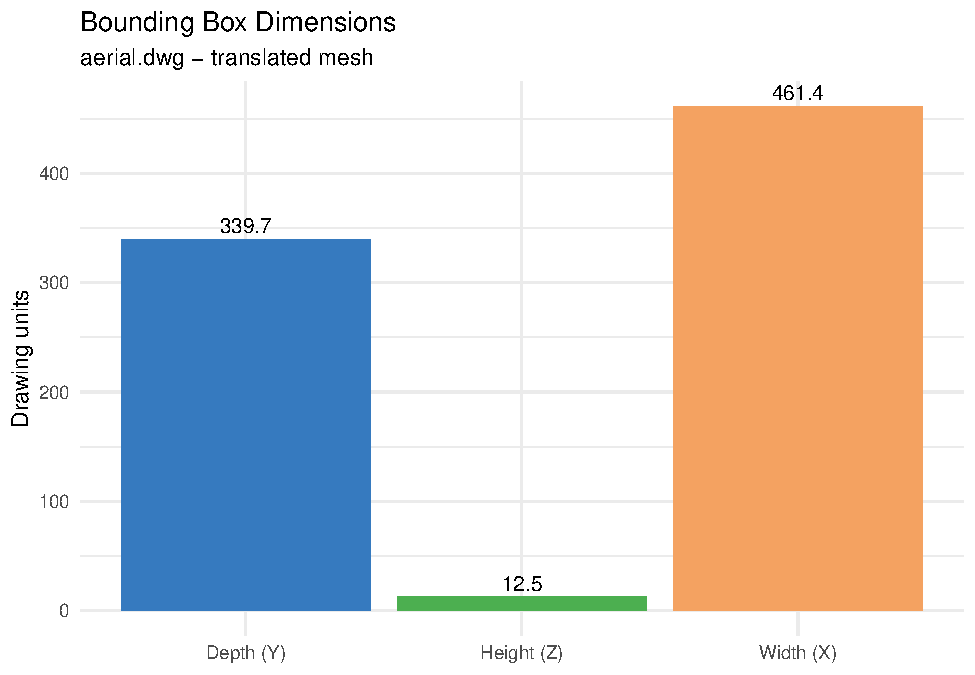
\includegraphics[keepaspectratio]{mesh-metrics_files/figure-pdf/unnamed-chunk-8-1.pdf}}

These metrics can be passed to a \texttt{gt} table for a polished
handover report. See \href{drawing-reports.qmd}{Automated Drawing
Reports} for the formatting details.

\chapter{3D Visualisation}\label{d-visualisation}

Numbers are useful; actually \emph{seeing} the mesh is better. This
chapter covers two routes: \texttt{rgl} (Adler, Murdoch, et al. 2024)
for interactive exploration in RStudio (spin it with the mouse, zoom in,
inspect details), and \texttt{rayshader} (Morgan-Wall 2024) for
rendering publication-quality static images.

Both work on \texttt{mesh\_vcg} from
\hyperref[reading-obj-and-stl-meshes]{Reading OBJ and STL Meshes}.

\section{Interactive 3D with rgl}\label{interactive-3d-with-rgl}

\texttt{shade3d()} opens an OpenGL window where you can rotate and zoom
with the mouse. Takes one line:

\begin{Shaded}
\begin{Highlighting}[]
\FunctionTok{library}\NormalTok{(rgl)}
\FunctionTok{open3d}\NormalTok{()}
\FunctionTok{shade3d}\NormalTok{(mesh\_obj, }\AttributeTok{col =} \StringTok{"\#C0C0C0"}\NormalTok{, }\AttributeTok{alpha =} \FloatTok{0.9}\NormalTok{)}
\FunctionTok{bg3d}\NormalTok{(}\StringTok{"white"}\NormalTok{)}
\FunctionTok{axes3d}\NormalTok{()}
\FunctionTok{title3d}\NormalTok{(}\StringTok{"Aerial DWG — Translated Mesh"}\NormalTok{)}
\end{Highlighting}
\end{Shaded}

\subsection{Embedding in HTML Output}\label{embedding-in-html-output}

\texttt{rgl} windows are interactive in RStudio but don't embed in HTML
documents on their own. \texttt{rglwidget()} wraps the scene in a
self-contained WebGL widget that works in any browser:

\begin{Shaded}
\begin{Highlighting}[]
\CommentTok{\# Add this once at the top of your document (setup chunk)}
\NormalTok{knitr}\SpecialCharTok{::}\NormalTok{knit\_hooks}\SpecialCharTok{$}\FunctionTok{set}\NormalTok{(}\AttributeTok{webgl =}\NormalTok{ rgl}\SpecialCharTok{::}\NormalTok{hook\_webgl)}

\FunctionTok{open3d}\NormalTok{()}
\FunctionTok{shade3d}\NormalTok{(mesh\_obj, }\AttributeTok{col =} \StringTok{"\#4A90D9"}\NormalTok{, }\AttributeTok{alpha =} \FloatTok{0.85}\NormalTok{)}
\FunctionTok{rglwidget}\NormalTok{()}
\end{Highlighting}
\end{Shaded}

\begin{tcolorbox}[enhanced jigsaw, titlerule=0mm, colback=white, colframe=quarto-callout-note-color-frame, bottomtitle=1mm, bottomrule=.15mm, coltitle=black, arc=.35mm, left=2mm, title=\textcolor{quarto-callout-note-color}{\faInfo}\hspace{0.5em}{Note}, colbacktitle=quarto-callout-note-color!10!white, toptitle=1mm, breakable, toprule=.15mm, rightrule=.15mm, leftrule=.75mm, opacitybacktitle=0.6, opacityback=0]

The WebGL widget is fully self-contained in the rendered HTML. Readers
can rotate and zoom without a running R server. It does require a modern
browser (Chrome, Firefox, Safari, Edge all work fine).

\end{tcolorbox}

\section{Colouring by Height}\label{colouring-by-height}

Map vertex Z-values to a colour ramp to reveal the model's vertical
structure instantly. Blues for low, reds for high:

\begin{Shaded}
\begin{Highlighting}[]
\NormalTok{z\_vals }\OtherTok{\textless{}{-}}\NormalTok{ mesh\_vcg}\SpecialCharTok{$}\NormalTok{vb[}\DecValTok{3}\NormalTok{, ]}
\NormalTok{z\_norm }\OtherTok{\textless{}{-}}\NormalTok{ (z\_vals }\SpecialCharTok{{-}} \FunctionTok{min}\NormalTok{(z\_vals)) }\SpecialCharTok{/} \FunctionTok{diff}\NormalTok{(}\FunctionTok{range}\NormalTok{(z\_vals))   }\CommentTok{\# 0–1}

\NormalTok{cols      }\OtherTok{\textless{}{-}} \FunctionTok{colorRampPalette}\NormalTok{(}\FunctionTok{c}\NormalTok{(}\StringTok{"\#2166ac"}\NormalTok{, }\StringTok{"\#92c5de"}\NormalTok{, }\StringTok{"\#f7f7f7"}\NormalTok{,}
                                 \StringTok{"\#f4a582"}\NormalTok{, }\StringTok{"\#d6604d"}\NormalTok{))(}\DecValTok{100}\NormalTok{)}
\NormalTok{vert\_cols }\OtherTok{\textless{}{-}}\NormalTok{ cols[}\FunctionTok{ceiling}\NormalTok{(z\_norm }\SpecialCharTok{*} \DecValTok{99}\NormalTok{) }\SpecialCharTok{+} \DecValTok{1}\NormalTok{]}

\FunctionTok{open3d}\NormalTok{()}
\FunctionTok{shade3d}\NormalTok{(mesh\_obj, }\AttributeTok{col =}\NormalTok{ vert\_cols)}
\FunctionTok{rglwidget}\NormalTok{()}
\end{Highlighting}
\end{Shaded}

\section{Rendered Images with
rayshader}\label{rendered-images-with-rayshader}

\texttt{rayshader} renders the active \texttt{rgl} scene with ray-traced
lighting and ambient occlusion, great for reports and presentations. The
output is a PNG file.

\begin{Shaded}
\begin{Highlighting}[]
\FunctionTok{library}\NormalTok{(rayshader)}

\NormalTok{vertices  }\OtherTok{\textless{}{-}} \FunctionTok{t}\NormalTok{(mesh\_vcg}\SpecialCharTok{$}\NormalTok{vb[}\DecValTok{1}\SpecialCharTok{:}\DecValTok{3}\NormalTok{, ])}
\NormalTok{triangles }\OtherTok{\textless{}{-}} \FunctionTok{t}\NormalTok{(mesh\_vcg}\SpecialCharTok{$}\NormalTok{it)}

\FunctionTok{open3d}\NormalTok{()}
\FunctionTok{triangles3d}\NormalTok{(vertices[triangles[, }\DecValTok{1}\NormalTok{], ],}
\NormalTok{            vertices[triangles[, }\DecValTok{2}\NormalTok{], ],}
\NormalTok{            vertices[triangles[, }\DecValTok{3}\NormalTok{], ],}
            \AttributeTok{col =} \StringTok{"steelblue"}\NormalTok{)}

\FunctionTok{render\_snapshot}\NormalTok{(}\AttributeTok{filename    =} \StringTok{"aerial\_render.png"}\NormalTok{,}
                \AttributeTok{width       =} \DecValTok{1200}\NormalTok{,}
                \AttributeTok{height      =} \DecValTok{900}\NormalTok{,}
                \AttributeTok{title\_text  =} \StringTok{"Aerial DWG — Rayshader Render"}\NormalTok{,}
                \AttributeTok{title\_color =} \StringTok{"white"}\NormalTok{,}
                \AttributeTok{title\_size  =} \DecValTok{24}\NormalTok{,}
                \AttributeTok{clear       =} \ConstantTok{TRUE}\NormalTok{)}
\end{Highlighting}
\end{Shaded}

Include the render in your Quarto document with a standard image link:

\begin{Shaded}
\begin{Highlighting}[]
\AlertTok{![Aerial DWG rendered with rayshader](aerial\_render.png)}
\end{Highlighting}
\end{Shaded}

\section{Depth of Field}\label{depth-of-field}

Add a depth-of-field effect to emphasise the model's 3D structure in the
output image, works especially well for tall structures:

\begin{Shaded}
\begin{Highlighting}[]
\FunctionTok{render\_depth}\NormalTok{(}\AttributeTok{focus       =} \FloatTok{0.7}\NormalTok{,}
             \AttributeTok{focallength =} \DecValTok{200}\NormalTok{,}
             \AttributeTok{filename    =} \StringTok{"aerial\_dof.png"}\NormalTok{)}
\end{Highlighting}
\end{Shaded}

\section{Quick Comparison: rgl
vs.~rayshader}\label{quick-comparison-rgl-vs.-rayshader}

\begin{longtable}[]{@{}lll@{}}
\toprule\noalign{}
& \texttt{rgl} & \texttt{rayshader} \\
\midrule\noalign{}
\endhead
\bottomrule\noalign{}
\endlastfoot
Output & Interactive HTML widget & Static PNG \\
Use for & Exploration, dashboards & Reports, presentations \\
Render time & Instant & Seconds--minutes \\
WebGL support & Yes (via \texttt{rglwidget()}) & No \\
\end{longtable}

\chapter{Point Cloud Analysis}\label{point-cloud-analysis}

The \hyperref[reality-capture]{Reality Capture} API can output a point
cloud alongside (or instead of) a mesh. Once you've converted it to LAS
format, \texttt{lidR} (Roussel et al. 2020) takes over --- height
statistics, density maps, canopy models, voxel volumes. This is the
go-to tool for site survey analysis.

\section{Getting the Point Cloud}\label{getting-the-point-cloud}

Request \texttt{rcs} format when creating your photoscene:

\begin{Shaded}
\begin{Highlighting}[]
\FunctionTok{library}\NormalTok{(AutoDeskR)}

\NormalTok{resp    }\OtherTok{\textless{}{-}} \FunctionTok{getToken}\NormalTok{(}\AttributeTok{id     =} \FunctionTok{Sys.getenv}\NormalTok{(}\StringTok{"client\_id"}\NormalTok{),}
                    \AttributeTok{secret =} \FunctionTok{Sys.getenv}\NormalTok{(}\StringTok{"client\_secret"}\NormalTok{),}
                    \AttributeTok{scope  =} \StringTok{"data:read data:write"}\NormalTok{)}
\NormalTok{myToken }\OtherTok{\textless{}{-}}\NormalTok{ resp}\SpecialCharTok{$}\NormalTok{content}\SpecialCharTok{$}\NormalTok{access\_token}

\NormalTok{ps }\OtherTok{\textless{}{-}} \FunctionTok{createPhotoscene}\NormalTok{(}\AttributeTok{name =} \StringTok{"site{-}2026{-}q2"}\NormalTok{, }\AttributeTok{token =}\NormalTok{ myToken)}
\CommentTok{\# ... uploadImages(), processPhotoscene(), waitForPhotoscene() ...}

\NormalTok{result  }\OtherTok{\textless{}{-}} \FunctionTok{checkPhotoscene}\NormalTok{(}\AttributeTok{photoscene\_id =}\NormalTok{ myPhotosceneId, }\AttributeTok{token =}\NormalTok{ myToken)}
\NormalTok{rcs\_url }\OtherTok{\textless{}{-}}\NormalTok{ result}\SpecialCharTok{$}\NormalTok{content}\SpecialCharTok{$}\NormalTok{photoscene}\SpecialCharTok{$}\NormalTok{scenelink}

\FunctionTok{download.file}\NormalTok{(}\AttributeTok{url      =}\NormalTok{ rcs\_url,}
              \AttributeTok{destfile =} \StringTok{"site{-}survey.rcs"}\NormalTok{,}
              \AttributeTok{headers  =} \FunctionTok{c}\NormalTok{(}\AttributeTok{Authorization =} \FunctionTok{paste}\NormalTok{(}\StringTok{"Bearer"}\NormalTok{, myToken)))}
\end{Highlighting}
\end{Shaded}

\begin{tcolorbox}[enhanced jigsaw, titlerule=0mm, colback=white, colframe=quarto-callout-warning-color-frame, bottomtitle=1mm, bottomrule=.15mm, coltitle=black, arc=.35mm, left=2mm, title=\textcolor{quarto-callout-warning-color}{\faExclamationTriangle}\hspace{0.5em}{Warning}, colbacktitle=quarto-callout-warning-color!10!white, toptitle=1mm, breakable, toprule=.15mm, rightrule=.15mm, leftrule=.75mm, opacitybacktitle=0.6, opacityback=0]

\textbf{\texttt{lidR} reads LAS/LAZ, not RCS.} Convert the downloaded
\texttt{.rcs} file to LAS using
\href{https://www.cloudcompare.org/}{CloudCompare} (free and open
source) before proceeding. In CloudCompare: \emph{File → Open} the RCS
file, then \emph{File → Save As} → LAS format.

\end{tcolorbox}

\section{Reading the Point Cloud}\label{reading-the-point-cloud}

\begin{Shaded}
\begin{Highlighting}[]
\FunctionTok{library}\NormalTok{(lidR)}
\NormalTok{pc }\OtherTok{\textless{}{-}} \FunctionTok{readLAS}\NormalTok{(}\StringTok{"site{-}survey.las"}\NormalTok{)}
\NormalTok{pc}
\CommentTok{\#\textgreater{} class        : LAS (v1.3 format 1)}
\CommentTok{\#\textgreater{} memory       : 247.8 Mb}
\CommentTok{\#\textgreater{} extent       : 406325.4, 406412.8, 5765842.6, 5765901.3}
\CommentTok{\#\textgreater{} coord. ref.  : WGS 84 / UTM zone 32N}
\CommentTok{\#\textgreater{} area         : 4064.9 units²}
\CommentTok{\#\textgreater{} points       : 3.62 million pts (1 return)}
\end{Highlighting}
\end{Shaded}

\section{Height Statistics}\label{height-statistics}

Normalise to ground level before computing anything height-related:

\begin{Shaded}
\begin{Highlighting}[]
\NormalTok{pc\_norm }\OtherTok{\textless{}{-}} \FunctionTok{normalize\_height}\NormalTok{(pc, }\FunctionTok{knnidw}\NormalTok{())}

\FunctionTok{mean}\NormalTok{(pc\_norm}\SpecialCharTok{$}\NormalTok{Z)}
\CommentTok{\#\textgreater{} [1] 4.12    \# mean height above ground (m)}
\FunctionTok{sd}\NormalTok{(pc\_norm}\SpecialCharTok{$}\NormalTok{Z)}
\CommentTok{\#\textgreater{} [1] 2.87}

\FunctionTok{quantile}\NormalTok{(pc\_norm}\SpecialCharTok{$}\NormalTok{Z, }\AttributeTok{probs =} \FunctionTok{c}\NormalTok{(}\FloatTok{0.25}\NormalTok{, }\FloatTok{0.5}\NormalTok{, }\FloatTok{0.75}\NormalTok{, }\FloatTok{0.95}\NormalTok{))}
\CommentTok{\#\textgreater{}   25\%   50\%   75\%   95\%}
\CommentTok{\#\textgreater{}  1.20  3.44  6.11 11.83}
\end{Highlighting}
\end{Shaded}

\section{Height Distribution}\label{height-distribution}

\begin{verbatim}
Warning: package 'ggplot2' was built under R version 4.4.3
\end{verbatim}

\begin{Shaded}
\begin{Highlighting}[]
\FunctionTok{ggplot}\NormalTok{(}\FunctionTok{data.frame}\NormalTok{(}\AttributeTok{z =}\NormalTok{ z\_sample), }\FunctionTok{aes}\NormalTok{(}\AttributeTok{x =}\NormalTok{ z)) }\SpecialCharTok{+}
  \FunctionTok{geom\_histogram}\NormalTok{(}\AttributeTok{binwidth =} \FloatTok{0.25}\NormalTok{, }\AttributeTok{fill =} \StringTok{"\#367ABF"}\NormalTok{, }\AttributeTok{colour =} \StringTok{"white"}\NormalTok{) }\SpecialCharTok{+}
  \FunctionTok{labs}\NormalTok{(}\AttributeTok{title =} \StringTok{"Point Cloud Height Distribution"}\NormalTok{,}
       \AttributeTok{subtitle =} \StringTok{"Normalised above ground level"}\NormalTok{,}
       \AttributeTok{x =} \StringTok{"Height (m)"}\NormalTok{, }\AttributeTok{y =} \StringTok{"Point count"}\NormalTok{) }\SpecialCharTok{+}
  \FunctionTok{theme\_minimal}\NormalTok{()}
\end{Highlighting}
\end{Shaded}

\pandocbounded{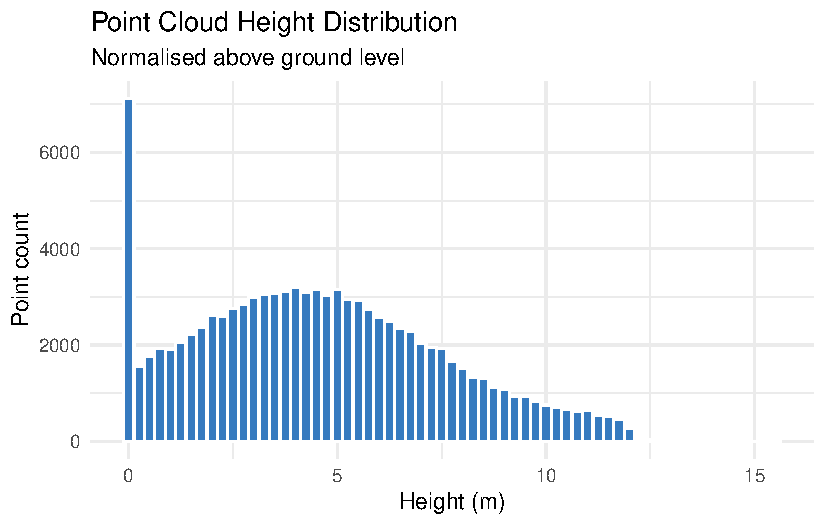
\includegraphics[keepaspectratio]{point-cloud-analysis_files/figure-pdf/unnamed-chunk-5-1.pdf}}

\section{Canopy Height Model}\label{canopy-height-model}

Rasterise the maximum Z per cell to produce a canopy height model ---
great for visualising roof heights or vegetation structure across the
site:

\begin{Shaded}
\begin{Highlighting}[]
\NormalTok{chm }\OtherTok{\textless{}{-}} \FunctionTok{rasterize\_canopy}\NormalTok{(pc\_norm, }\AttributeTok{res =} \FloatTok{0.5}\NormalTok{, }\AttributeTok{algorithm =} \FunctionTok{p2r}\NormalTok{())}
\FunctionTok{plot}\NormalTok{(chm, }\AttributeTok{col =} \FunctionTok{height.colors}\NormalTok{(}\DecValTok{50}\NormalTok{), }\AttributeTok{main =} \StringTok{"Canopy Height Model (0.5 m resolution)"}\NormalTok{)}
\end{Highlighting}
\end{Shaded}

\section{Point Density Grid}\label{point-density-grid}

\begin{Shaded}
\begin{Highlighting}[]
\NormalTok{density }\OtherTok{\textless{}{-}} \FunctionTok{grid\_density}\NormalTok{(pc, }\AttributeTok{res =} \DecValTok{1}\NormalTok{)}
\FunctionTok{plot}\NormalTok{(density, }\AttributeTok{col =} \FunctionTok{gray.colors}\NormalTok{(}\DecValTok{50}\NormalTok{), }\AttributeTok{main =} \StringTok{"Point Density (pts/m²)"}\NormalTok{)}

\FunctionTok{mean}\NormalTok{(density[], }\AttributeTok{na.rm =} \ConstantTok{TRUE}\NormalTok{)}
\CommentTok{\#\textgreater{} [1] 891.3   \# points per square metre}
\end{Highlighting}
\end{Shaded}

\section{Voxel Volume}\label{voxel-volume}

\begin{Shaded}
\begin{Highlighting}[]
\NormalTok{vox        }\OtherTok{\textless{}{-}} \FunctionTok{voxelize\_points}\NormalTok{(pc\_norm, }\AttributeTok{res =} \FloatTok{0.25}\NormalTok{)}
\NormalTok{volume\_m3  }\OtherTok{\textless{}{-}} \FunctionTok{nrow}\NormalTok{(vox) }\SpecialCharTok{*} \FloatTok{0.25}\SpecialCharTok{\^{}}\DecValTok{3}
\FunctionTok{cat}\NormalTok{(}\StringTok{"Estimated volume:"}\NormalTok{, }\FunctionTok{round}\NormalTok{(volume\_m3, }\DecValTok{1}\NormalTok{), }\StringTok{"m³}\SpecialCharTok{\textbackslash{}n}\StringTok{"}\NormalTok{)}
\CommentTok{\#\textgreater{} Estimated volume: 1483.2 m³}
\end{Highlighting}
\end{Shaded}

\section{Summary Table}\label{summary-table-1}

\begin{Shaded}
\begin{Highlighting}[]
\FunctionTok{library}\NormalTok{(ggplot2)}

\NormalTok{metrics }\OtherTok{\textless{}{-}} \FunctionTok{data.frame}\NormalTok{(}
  \AttributeTok{metric =} \FunctionTok{c}\NormalTok{(}\StringTok{"Total points"}\NormalTok{, }\StringTok{"Survey area (m²)"}\NormalTok{, }\StringTok{"Mean density (pts/m²)"}\NormalTok{,}
             \StringTok{"Mean height (m)"}\NormalTok{, }\StringTok{"95th{-}pct height (m)"}\NormalTok{, }\StringTok{"Voxel volume (m³)"}\NormalTok{),}
  \AttributeTok{value  =} \FunctionTok{c}\NormalTok{(}\FunctionTok{npoints}\NormalTok{(pc), }\FunctionTok{area}\NormalTok{(pc), }\FunctionTok{mean}\NormalTok{(density[], }\AttributeTok{na.rm =} \ConstantTok{TRUE}\NormalTok{),}
             \FunctionTok{mean}\NormalTok{(pc\_norm}\SpecialCharTok{$}\NormalTok{Z), }\FunctionTok{quantile}\NormalTok{(pc\_norm}\SpecialCharTok{$}\NormalTok{Z, }\FloatTok{0.95}\NormalTok{), volume\_m3)}
\NormalTok{)}

\FunctionTok{ggplot}\NormalTok{(metrics, }\FunctionTok{aes}\NormalTok{(}\AttributeTok{x =} \FunctionTok{reorder}\NormalTok{(metric, value), }\AttributeTok{y =}\NormalTok{ value)) }\SpecialCharTok{+}
  \FunctionTok{geom\_col}\NormalTok{(}\AttributeTok{fill =} \StringTok{"\#367ABF"}\NormalTok{) }\SpecialCharTok{+}
  \FunctionTok{coord\_flip}\NormalTok{() }\SpecialCharTok{+}
  \FunctionTok{labs}\NormalTok{(}\AttributeTok{title =} \StringTok{"Point Cloud Summary Metrics"}\NormalTok{,}
       \AttributeTok{x =} \ConstantTok{NULL}\NormalTok{, }\AttributeTok{y =} \StringTok{"Value"}\NormalTok{) }\SpecialCharTok{+}
  \FunctionTok{theme\_minimal}\NormalTok{()}
\end{Highlighting}
\end{Shaded}

\chapter{Mesh Comparison}\label{mesh-comparison}

As-designed vs.~as-built: did the construction actually match the model?
\texttt{Rvcg} (Schlager 2024) lets you quantify that gap by computing
per-vertex surface distances between two meshes, and colour the design
mesh by how far each point drifted.

The typical setup: the design mesh comes from a DWG translated via the
\hyperref[model-derivative]{Model Derivative} API; the as-built mesh
comes from \hyperref[reality-capture]{Reality Capture} photogrammetry.

\section{Loading Two Meshes}\label{loading-two-meshes}

\begin{Shaded}
\begin{Highlighting}[]
\FunctionTok{library}\NormalTok{(Rvcg)}

\NormalTok{mesh\_design }\OtherTok{\textless{}{-}} \FunctionTok{vcgImport}\NormalTok{(}\StringTok{"aerial\_design.obj"}\NormalTok{)   }\CommentTok{\# as{-}designed}
\NormalTok{mesh\_built  }\OtherTok{\textless{}{-}} \FunctionTok{vcgImport}\NormalTok{(}\StringTok{"aerial\_asbuilt.obj"}\NormalTok{)  }\CommentTok{\# from Reality Capture}

\FunctionTok{cat}\NormalTok{(}\StringTok{"Design vertices:  "}\NormalTok{, }\FunctionTok{ncol}\NormalTok{(mesh\_design}\SpecialCharTok{$}\NormalTok{vb), }\StringTok{"}\SpecialCharTok{\textbackslash{}n}\StringTok{"}\NormalTok{)}
\CommentTok{\#\textgreater{} Design vertices:   2847}
\FunctionTok{cat}\NormalTok{(}\StringTok{"As{-}built vertices:"}\NormalTok{, }\FunctionTok{ncol}\NormalTok{(mesh\_built}\SpecialCharTok{$}\NormalTok{vb),  }\StringTok{"}\SpecialCharTok{\textbackslash{}n}\StringTok{"}\NormalTok{)}
\CommentTok{\#\textgreater{} As{-}built vertices: 38124}
\end{Highlighting}
\end{Shaded}

\section{Smoothing the As-Built Mesh}\label{smoothing-the-as-built-mesh}

Photogrammetric meshes carry surface noise from image reconstruction. A
few iterations of Laplacian smoothing tames that without destroying the
coarse geometry:

\begin{Shaded}
\begin{Highlighting}[]
\NormalTok{mesh\_built\_smooth }\OtherTok{\textless{}{-}} \FunctionTok{vcgSmooth}\NormalTok{(mesh\_built, }\AttributeTok{iteration =} \DecValTok{3}\NormalTok{, }\AttributeTok{lambda =} \FloatTok{0.5}\NormalTok{)}
\end{Highlighting}
\end{Shaded}

\section{Surface Distance}\label{surface-distance}

\texttt{vcgDist()} computes, for each vertex of the first mesh, the
distance to the nearest point on the surface of the second mesh:

\begin{Shaded}
\begin{Highlighting}[]
\NormalTok{dist\_result }\OtherTok{\textless{}{-}} \FunctionTok{vcgDist}\NormalTok{(mesh\_design, mesh\_built\_smooth)}

\FunctionTok{summary}\NormalTok{(dist\_result}\SpecialCharTok{$}\NormalTok{distances)}
\CommentTok{\#\textgreater{}    Min. 1st Qu.  Median    Mean 3rd Qu.    Max.}
\CommentTok{\#\textgreater{}   0.000   0.021   0.089   0.143   0.198   4.782}
\end{Highlighting}
\end{Shaded}

\section{Deviation Colour Map}\label{deviation-colour-map}

Map the distances to a blue--white--red ramp and render the design mesh
coloured by deviation. Clip the colour scale at 0.5 m. Anything beyond
that is shown as maximum red so extreme outliers don't wash out the
detail:

\begin{Shaded}
\begin{Highlighting}[]
\FunctionTok{library}\NormalTok{(rgl)}

\NormalTok{cols      }\OtherTok{\textless{}{-}} \FunctionTok{colorRampPalette}\NormalTok{(}\FunctionTok{c}\NormalTok{(}\StringTok{"\#2166ac"}\NormalTok{, }\StringTok{"\#f7f7f7"}\NormalTok{, }\StringTok{"\#d6604d"}\NormalTok{))(}\DecValTok{100}\NormalTok{)}
\NormalTok{d\_norm    }\OtherTok{\textless{}{-}} \FunctionTok{pmin}\NormalTok{(dist\_result}\SpecialCharTok{$}\NormalTok{distances }\SpecialCharTok{/} \FloatTok{0.5}\NormalTok{, }\DecValTok{1}\NormalTok{)}
\NormalTok{vert\_cols }\OtherTok{\textless{}{-}}\NormalTok{ cols[}\FunctionTok{ceiling}\NormalTok{(d\_norm }\SpecialCharTok{*} \DecValTok{99}\NormalTok{) }\SpecialCharTok{+} \DecValTok{1}\NormalTok{]}

\FunctionTok{open3d}\NormalTok{()}
\FunctionTok{shade3d}\NormalTok{(mesh\_design, }\AttributeTok{col =}\NormalTok{ vert\_cols)}
\FunctionTok{rglwidget}\NormalTok{()}
\end{Highlighting}
\end{Shaded}

\section{Summary Statistics}\label{summary-statistics}

\begin{Shaded}
\begin{Highlighting}[]
\NormalTok{d }\OtherTok{\textless{}{-}}\NormalTok{ dist\_result}\SpecialCharTok{$}\NormalTok{distances}

\NormalTok{deviation\_summary }\OtherTok{\textless{}{-}} \FunctionTok{data.frame}\NormalTok{(}
  \AttributeTok{metric =} \FunctionTok{c}\NormalTok{(}\StringTok{"Max deviation (m)"}\NormalTok{, }\StringTok{"Mean deviation (m)"}\NormalTok{,}
             \StringTok{"RMS deviation (m)"}\NormalTok{, }\StringTok{"\% vertices \textgreater{} 50 mm"}\NormalTok{,}
             \StringTok{"\% vertices \textgreater{} 100 mm"}\NormalTok{),}
  \AttributeTok{value  =} \FunctionTok{round}\NormalTok{(}\FunctionTok{c}\NormalTok{(}\FunctionTok{max}\NormalTok{(d), }\FunctionTok{mean}\NormalTok{(d), }\FunctionTok{sqrt}\NormalTok{(}\FunctionTok{mean}\NormalTok{(d}\SpecialCharTok{\^{}}\DecValTok{2}\NormalTok{)),}
                   \DecValTok{100} \SpecialCharTok{*} \FunctionTok{mean}\NormalTok{(d }\SpecialCharTok{\textgreater{}} \FloatTok{0.05}\NormalTok{),}
                   \DecValTok{100} \SpecialCharTok{*} \FunctionTok{mean}\NormalTok{(d }\SpecialCharTok{\textgreater{}} \FloatTok{0.10}\NormalTok{)), }\DecValTok{3}\NormalTok{)}
\NormalTok{)}
\NormalTok{deviation\_summary}
\CommentTok{\#\textgreater{}                 metric  value}
\CommentTok{\#\textgreater{} 1    Max deviation (m)  4.782}
\CommentTok{\#\textgreater{} 2   Mean deviation (m)  0.143}
\CommentTok{\#\textgreater{} 3    RMS deviation (m)  0.221}
\CommentTok{\#\textgreater{} 4  \% vertices \textgreater{} 50 mm 34.200}
\CommentTok{\#\textgreater{} 5 \% vertices \textgreater{} 100 mm 18.700}
\end{Highlighting}
\end{Shaded}

\begin{tcolorbox}[enhanced jigsaw, titlerule=0mm, colback=white, colframe=quarto-callout-tip-color-frame, bottomtitle=1mm, bottomrule=.15mm, coltitle=black, arc=.35mm, left=2mm, title=\textcolor{quarto-callout-tip-color}{\faLightbulb}\hspace{0.5em}{Tip}, colbacktitle=quarto-callout-tip-color!10!white, toptitle=1mm, breakable, toprule=.15mm, rightrule=.15mm, leftrule=.75mm, opacitybacktitle=0.6, opacityback=0]

A mean deviation below 50 mm (0.05 m) is generally acceptable for
architectural construction tolerances. Structural and civil works often
require tighter thresholds. Always check the project specification
before drawing conclusions.

\end{tcolorbox}

\section{Deviation Histogram}\label{deviation-histogram}

A histogram puts the distribution in context and makes it easy to spot
whether deviations are concentrated in one area or spread uniformly
across the model:

\begin{verbatim}
Warning: package 'ggplot2' was built under R version 4.4.3
\end{verbatim}

\begin{Shaded}
\begin{Highlighting}[]
\FunctionTok{ggplot}\NormalTok{(}\FunctionTok{data.frame}\NormalTok{(}\AttributeTok{deviation\_mm =}\NormalTok{ d }\SpecialCharTok{*} \DecValTok{1000}\NormalTok{), }\FunctionTok{aes}\NormalTok{(}\AttributeTok{x =}\NormalTok{ deviation\_mm)) }\SpecialCharTok{+}
  \FunctionTok{geom\_histogram}\NormalTok{(}\AttributeTok{binwidth =} \DecValTok{5}\NormalTok{, }\AttributeTok{fill =} \StringTok{"\#367ABF"}\NormalTok{, }\AttributeTok{colour =} \StringTok{"white"}\NormalTok{) }\SpecialCharTok{+}
  \FunctionTok{geom\_vline}\NormalTok{(}\AttributeTok{xintercept =} \DecValTok{50}\NormalTok{, }\AttributeTok{linetype =} \StringTok{"dashed"}\NormalTok{, }\AttributeTok{colour =} \StringTok{"\#d6604d"}\NormalTok{, }\AttributeTok{linewidth =} \FloatTok{0.8}\NormalTok{) }\SpecialCharTok{+}
  \FunctionTok{annotate}\NormalTok{(}\StringTok{"text"}\NormalTok{, }\AttributeTok{x =} \DecValTok{55}\NormalTok{, }\AttributeTok{y =} \ConstantTok{Inf}\NormalTok{, }\AttributeTok{label =} \StringTok{"50 mm tolerance"}\NormalTok{,}
           \AttributeTok{hjust =} \DecValTok{0}\NormalTok{, }\AttributeTok{vjust =} \FloatTok{1.5}\NormalTok{, }\AttributeTok{colour =} \StringTok{"\#d6604d"}\NormalTok{, }\AttributeTok{size =} \FloatTok{3.5}\NormalTok{) }\SpecialCharTok{+}
  \FunctionTok{labs}\NormalTok{(}\AttributeTok{title =} \StringTok{"As{-}Designed vs. As{-}Built Deviation"}\NormalTok{,}
       \AttributeTok{subtitle =} \StringTok{"Per{-}vertex surface distance"}\NormalTok{,}
       \AttributeTok{x =} \StringTok{"Deviation (mm)"}\NormalTok{,}
       \AttributeTok{y =} \StringTok{"Vertex count"}\NormalTok{) }\SpecialCharTok{+}
  \FunctionTok{theme\_minimal}\NormalTok{()}
\end{Highlighting}
\end{Shaded}

\pandocbounded{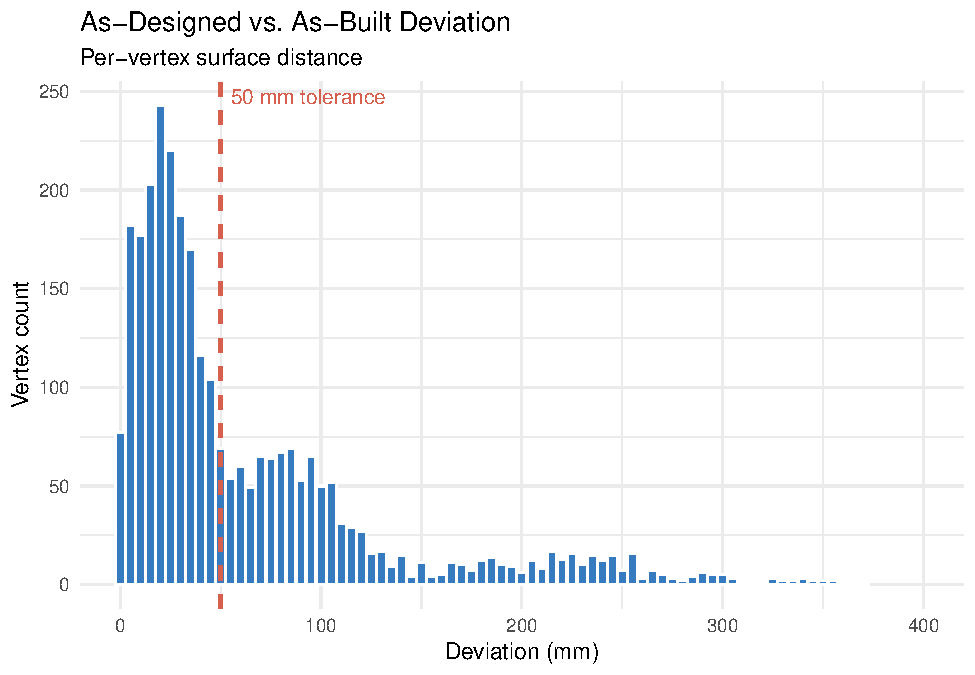
\includegraphics[keepaspectratio]{mesh-comparison_files/figure-pdf/unnamed-chunk-7-1.pdf}}

\section{Cumulative Distribution}\label{cumulative-distribution}

A CDF plot tells you what fraction of the model is within any given
tolerance, handy for pass/fail reporting:

\begin{Shaded}
\begin{Highlighting}[]
\FunctionTok{ggplot}\NormalTok{(}\FunctionTok{data.frame}\NormalTok{(}\AttributeTok{deviation\_mm =} \FunctionTok{sort}\NormalTok{(d }\SpecialCharTok{*} \DecValTok{1000}\NormalTok{)),}
       \FunctionTok{aes}\NormalTok{(}\AttributeTok{x =}\NormalTok{ deviation\_mm, }\AttributeTok{y =} \FunctionTok{seq\_along}\NormalTok{(deviation\_mm) }\SpecialCharTok{/} \FunctionTok{length}\NormalTok{(d) }\SpecialCharTok{*} \DecValTok{100}\NormalTok{)) }\SpecialCharTok{+}
  \FunctionTok{geom\_line}\NormalTok{(}\AttributeTok{colour =} \StringTok{"\#367ABF"}\NormalTok{, }\AttributeTok{linewidth =} \FloatTok{0.9}\NormalTok{) }\SpecialCharTok{+}
  \FunctionTok{geom\_vline}\NormalTok{(}\AttributeTok{xintercept =} \DecValTok{50}\NormalTok{, }\AttributeTok{linetype =} \StringTok{"dashed"}\NormalTok{, }\AttributeTok{colour =} \StringTok{"\#d6604d"}\NormalTok{) }\SpecialCharTok{+}
  \FunctionTok{geom\_hline}\NormalTok{(}\AttributeTok{yintercept =} \DecValTok{100} \SpecialCharTok{*} \FunctionTok{mean}\NormalTok{(d }\SpecialCharTok{\textless{}=} \FloatTok{0.05}\NormalTok{),}
             \AttributeTok{linetype =} \StringTok{"dotted"}\NormalTok{, }\AttributeTok{colour =} \StringTok{"\#4CAF50"}\NormalTok{) }\SpecialCharTok{+}
  \FunctionTok{labs}\NormalTok{(}\AttributeTok{title =} \StringTok{"Cumulative Deviation Distribution"}\NormalTok{,}
       \AttributeTok{x =} \StringTok{"Deviation (mm)"}\NormalTok{,}
       \AttributeTok{y =} \StringTok{"\% of vertices"}\NormalTok{) }\SpecialCharTok{+}
  \FunctionTok{theme\_minimal}\NormalTok{()}
\end{Highlighting}
\end{Shaded}

\pandocbounded{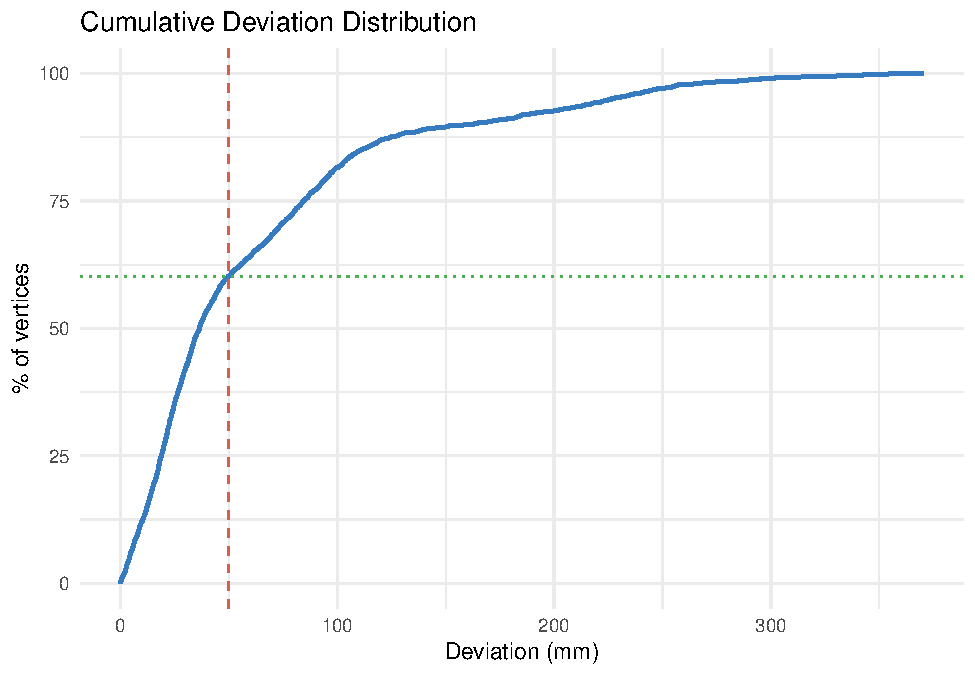
\includegraphics[keepaspectratio]{mesh-comparison_files/figure-pdf/unnamed-chunk-8-1.pdf}}

\part{DWG \& DXF Analytics}

\chapter{Layer Structure Analysis}\label{layer-structure-analysis}

Every DWG and DXF file organises its geometry into named layers. Unlock
those layers through the \hyperref[model-derivative]{Model Derivative}
API and you've got a structured dataset ready for \texttt{dplyr}. This
chapter extracts per-layer element counts and areas and charts them ---
no CAD software required.

The data flows like this:

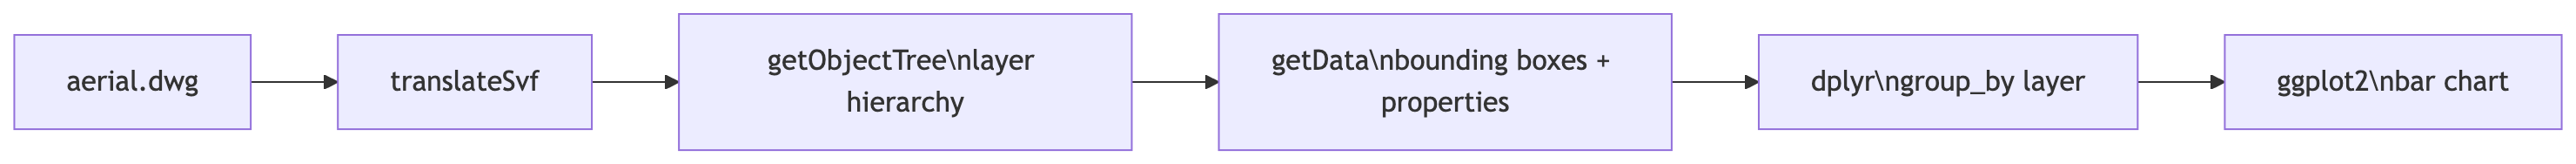
\includegraphics[width=15.4in,height=0.98in]{layer-analysis_files/figure-latex/mermaid-figure-1.png}

\section{Prerequisites}\label{prerequisites-2}

\begin{Shaded}
\begin{Highlighting}[]
\FunctionTok{install.packages}\NormalTok{(}\FunctionTok{c}\NormalTok{(}\StringTok{"dplyr"}\NormalTok{, }\StringTok{"ggplot2"}\NormalTok{))}
\end{Highlighting}
\end{Shaded}

\section{Authenticate and Translate}\label{authenticate-and-translate}

SVF format is what unlocks metadata access --- translate first, then
query:

\begin{Shaded}
\begin{Highlighting}[]
\FunctionTok{library}\NormalTok{(AutoDeskR)}
\FunctionTok{library}\NormalTok{(dplyr)}

\NormalTok{resp     }\OtherTok{\textless{}{-}} \FunctionTok{getToken}\NormalTok{(}\AttributeTok{id     =} \FunctionTok{Sys.getenv}\NormalTok{(}\StringTok{"client\_id"}\NormalTok{),}
                     \AttributeTok{secret =} \FunctionTok{Sys.getenv}\NormalTok{(}\StringTok{"client\_secret"}\NormalTok{),}
                     \AttributeTok{scope  =} \StringTok{"data:read data:write"}\NormalTok{)}
\NormalTok{myToken  }\OtherTok{\textless{}{-}}\NormalTok{ resp}\SpecialCharTok{$}\NormalTok{content}\SpecialCharTok{$}\NormalTok{access\_token}

\NormalTok{myEncodedUrn }\OtherTok{\textless{}{-}}\NormalTok{ jsonlite}\SpecialCharTok{::}\FunctionTok{base64\_enc}\NormalTok{(}\FunctionTok{Sys.getenv}\NormalTok{(}\StringTok{"urn"}\NormalTok{))}
\FunctionTok{translateSvf}\NormalTok{(}\AttributeTok{urn =}\NormalTok{ myEncodedUrn, }\AttributeTok{token =}\NormalTok{ myToken)}

\ControlFlowTok{repeat}\NormalTok{ \{}
\NormalTok{  status }\OtherTok{\textless{}{-}} \FunctionTok{checkFile}\NormalTok{(}\AttributeTok{urn =}\NormalTok{ myEncodedUrn, }\AttributeTok{token =}\NormalTok{ myToken)}
  \ControlFlowTok{if}\NormalTok{ (status}\SpecialCharTok{$}\NormalTok{content}\SpecialCharTok{$}\NormalTok{status }\SpecialCharTok{==} \StringTok{"success"}\NormalTok{) }\ControlFlowTok{break}
  \FunctionTok{Sys.sleep}\NormalTok{(}\DecValTok{5}\NormalTok{)}
\NormalTok{\}}

\NormalTok{resp\_meta }\OtherTok{\textless{}{-}} \FunctionTok{getMetadata}\NormalTok{(}\AttributeTok{urn =}\NormalTok{ myEncodedUrn, }\AttributeTok{token =}\NormalTok{ myToken)}
\NormalTok{myGuid    }\OtherTok{\textless{}{-}}\NormalTok{ resp\_meta}\SpecialCharTok{$}\NormalTok{content}\SpecialCharTok{$}\NormalTok{data}\SpecialCharTok{$}\NormalTok{metadata[[}\DecValTok{1}\NormalTok{]]}\SpecialCharTok{$}\NormalTok{guid}
\end{Highlighting}
\end{Shaded}

\section{The Object Tree}\label{the-object-tree}

\texttt{getObjectTree()} returns the model hierarchy. In a DWG, the root
node's children are the layers:

\begin{Shaded}
\begin{Highlighting}[]
\NormalTok{tree\_resp }\OtherTok{\textless{}{-}} \FunctionTok{getObjectTree}\NormalTok{(}\AttributeTok{guid =}\NormalTok{ myGuid, }\AttributeTok{urn =}\NormalTok{ myEncodedUrn, }\AttributeTok{token =}\NormalTok{ myToken)}
\NormalTok{root      }\OtherTok{\textless{}{-}}\NormalTok{ tree\_resp}\SpecialCharTok{$}\NormalTok{content}\SpecialCharTok{$}\NormalTok{data}\SpecialCharTok{$}\NormalTok{objects[[}\DecValTok{1}\NormalTok{]]}

\NormalTok{root}\SpecialCharTok{$}\NormalTok{objects[[}\DecValTok{1}\NormalTok{]]}
\CommentTok{\#\textgreater{} $objectid [1] 2}
\CommentTok{\#\textgreater{} $name     [1] "Layer: A{-}SITE"}
\CommentTok{\#\textgreater{} $objects       \# geometry objects on this layer}
\end{Highlighting}
\end{Shaded}

\section{Flatten the Tree}\label{flatten-the-tree}

A small recursive helper turns the nested list into a tidy data frame
--- one row per leaf object:

\begin{Shaded}
\begin{Highlighting}[]
\NormalTok{flatten\_tree }\OtherTok{\textless{}{-}} \ControlFlowTok{function}\NormalTok{(node, }\AttributeTok{parent\_layer =} \ConstantTok{NA\_character\_}\NormalTok{) \{}
\NormalTok{  is\_layer   }\OtherTok{\textless{}{-}} \FunctionTok{grepl}\NormalTok{(}\StringTok{"\^{}Layer:"}\NormalTok{, node}\SpecialCharTok{$}\NormalTok{name)}
\NormalTok{  layer\_name }\OtherTok{\textless{}{-}} \ControlFlowTok{if}\NormalTok{ (is\_layer) }\FunctionTok{sub}\NormalTok{(}\StringTok{"\^{}Layer: "}\NormalTok{, }\StringTok{""}\NormalTok{, node}\SpecialCharTok{$}\NormalTok{name) }\ControlFlowTok{else}\NormalTok{ parent\_layer}
  \ControlFlowTok{if}\NormalTok{ (}\FunctionTok{is.null}\NormalTok{(node}\SpecialCharTok{$}\NormalTok{objects)) \{}
    \FunctionTok{return}\NormalTok{(}\FunctionTok{data.frame}\NormalTok{(}\AttributeTok{objectid =}\NormalTok{ node}\SpecialCharTok{$}\NormalTok{objectid,}
                      \AttributeTok{name     =}\NormalTok{ node}\SpecialCharTok{$}\NormalTok{name,}
                      \AttributeTok{layer    =}\NormalTok{ layer\_name,}
                      \AttributeTok{stringsAsFactors =} \ConstantTok{FALSE}\NormalTok{))}
\NormalTok{  \}}
  \FunctionTok{do.call}\NormalTok{(rbind, }\FunctionTok{lapply}\NormalTok{(node}\SpecialCharTok{$}\NormalTok{objects, flatten\_tree, }\AttributeTok{parent\_layer =}\NormalTok{ layer\_name))}
\NormalTok{\}}

\NormalTok{tree\_df }\OtherTok{\textless{}{-}} \FunctionTok{flatten\_tree}\NormalTok{(root)}
\FunctionTok{head}\NormalTok{(tree\_df)}
\CommentTok{\#\textgreater{}   objectid              name   layer}
\CommentTok{\#\textgreater{} 1        5  Polyline (closed)  A{-}SITE}
\CommentTok{\#\textgreater{} 2        6  Polyline (closed)  A{-}SITE}
\CommentTok{\#\textgreater{} 3       12              Line  A{-}BLDG}
\end{Highlighting}
\end{Shaded}

\section{Extract Properties with
getData()}\label{extract-properties-with-getdata}

\texttt{getData()} returns the full property set for every object ---
including bounding box coordinates:

\begin{Shaded}
\begin{Highlighting}[]
\NormalTok{data\_resp  }\OtherTok{\textless{}{-}} \FunctionTok{getData}\NormalTok{(}\AttributeTok{guid =}\NormalTok{ myGuid, }\AttributeTok{urn =}\NormalTok{ myEncodedUrn, }\AttributeTok{token =}\NormalTok{ myToken)}
\NormalTok{collection }\OtherTok{\textless{}{-}}\NormalTok{ data\_resp}\SpecialCharTok{$}\NormalTok{content}\SpecialCharTok{$}\NormalTok{data}\SpecialCharTok{$}\NormalTok{collection}

\NormalTok{props\_df }\OtherTok{\textless{}{-}} \FunctionTok{lapply}\NormalTok{(collection, }\ControlFlowTok{function}\NormalTok{(obj) \{}
\NormalTok{  geom }\OtherTok{\textless{}{-}}\NormalTok{ obj}\SpecialCharTok{$}\NormalTok{properties}\SpecialCharTok{$}\NormalTok{Geometry}
  \FunctionTok{data.frame}\NormalTok{(}
    \AttributeTok{objectid =}\NormalTok{ obj}\SpecialCharTok{$}\NormalTok{objectid,}
    \AttributeTok{layer    =}\NormalTok{ obj}\SpecialCharTok{$}\NormalTok{properties[[}\StringTok{"Layer and Material"}\NormalTok{]][[}\StringTok{"Layer"}\NormalTok{]],}
    \AttributeTok{bb\_min\_x =}\NormalTok{ geom[[}\StringTok{"Bounding Box Min X"}\NormalTok{]],}
    \AttributeTok{bb\_min\_y =}\NormalTok{ geom[[}\StringTok{"Bounding Box Min Y"}\NormalTok{]],}
    \AttributeTok{bb\_max\_x =}\NormalTok{ geom[[}\StringTok{"Bounding Box Max X"}\NormalTok{]],}
    \AttributeTok{bb\_max\_y =}\NormalTok{ geom[[}\StringTok{"Bounding Box Max Y"}\NormalTok{]],}
    \AttributeTok{stringsAsFactors =} \ConstantTok{FALSE}
\NormalTok{  )}
\NormalTok{\}) }\SpecialCharTok{|\textgreater{}} \FunctionTok{do.call}\NormalTok{(}\AttributeTok{what =}\NormalTok{ rbind)}

\NormalTok{props\_df }\OtherTok{\textless{}{-}}\NormalTok{ props\_df }\SpecialCharTok{|\textgreater{}}
  \FunctionTok{mutate}\NormalTok{(}\AttributeTok{bb\_area =}\NormalTok{ (bb\_max\_x }\SpecialCharTok{{-}}\NormalTok{ bb\_min\_x) }\SpecialCharTok{*}\NormalTok{ (bb\_max\_y }\SpecialCharTok{{-}}\NormalTok{ bb\_min\_y))}
\end{Highlighting}
\end{Shaded}

\begin{tcolorbox}[enhanced jigsaw, titlerule=0mm, colback=white, colframe=quarto-callout-warning-color-frame, bottomtitle=1mm, bottomrule=.15mm, coltitle=black, arc=.35mm, left=2mm, title=\textcolor{quarto-callout-warning-color}{\faExclamationTriangle}\hspace{0.5em}{Warning}, colbacktitle=quarto-callout-warning-color!10!white, toptitle=1mm, breakable, toprule=.15mm, rightrule=.15mm, leftrule=.75mm, opacitybacktitle=0.6, opacityback=0]

Complex DWGs can return thousands of objects from \texttt{getData()}.
For large files, pre-filter the object tree to the layers you care about
before calling it to keep response sizes manageable.

\end{tcolorbox}

\section{Summarise by Layer}\label{summarise-by-layer}

\begin{Shaded}
\begin{Highlighting}[]
\NormalTok{layer\_summary }\OtherTok{\textless{}{-}}\NormalTok{ props\_df }\SpecialCharTok{|\textgreater{}}
  \FunctionTok{group\_by}\NormalTok{(layer) }\SpecialCharTok{|\textgreater{}}
  \FunctionTok{summarise}\NormalTok{(}\AttributeTok{n\_objects  =} \FunctionTok{n}\NormalTok{(),}
            \AttributeTok{total\_area =} \FunctionTok{sum}\NormalTok{(bb\_area, }\AttributeTok{na.rm =} \ConstantTok{TRUE}\NormalTok{),}
            \AttributeTok{mean\_area  =} \FunctionTok{mean}\NormalTok{(bb\_area, }\AttributeTok{na.rm =} \ConstantTok{TRUE}\NormalTok{),}
            \AttributeTok{.groups    =} \StringTok{"drop"}\NormalTok{) }\SpecialCharTok{|\textgreater{}}
  \FunctionTok{arrange}\NormalTok{(}\FunctionTok{desc}\NormalTok{(total\_area))}

\NormalTok{layer\_summary}
\CommentTok{\#\textgreater{} \# A tibble: 8 × 4}
\CommentTok{\#\textgreater{}   layer    n\_objects total\_area mean\_area}
\CommentTok{\#\textgreater{}   \textless{}chr\textgreater{}        \textless{}int\textgreater{}      \textless{}dbl\textgreater{}     \textless{}dbl\textgreater{}}
\CommentTok{\#\textgreater{} 1 A{-}SITE          34    156823.    4612.}
\CommentTok{\#\textgreater{} 2 A{-}BLDG          21     89341.    4254.}
\CommentTok{\#\textgreater{} 3 A{-}ROAD          12     43218.    3601.}
\CommentTok{\#\textgreater{} 4 A{-}HATCH          8     12044.    1506.}
\CommentTok{\#\textgreater{} 5 A{-}TEXT          47      4831.     103.}
\end{Highlighting}
\end{Shaded}

\section{Area by Layer --- Bar Chart}\label{area-by-layer-bar-chart}

\begin{verbatim}
Warning: package 'ggplot2' was built under R version 4.4.3
\end{verbatim}

\begin{Shaded}
\begin{Highlighting}[]
\FunctionTok{ggplot}\NormalTok{(layer\_summary,}
       \FunctionTok{aes}\NormalTok{(}\AttributeTok{x =} \FunctionTok{reorder}\NormalTok{(layer, total\_area), }\AttributeTok{y =}\NormalTok{ total\_area }\SpecialCharTok{/} \DecValTok{1000}\NormalTok{)) }\SpecialCharTok{+}
  \FunctionTok{geom\_col}\NormalTok{(}\AttributeTok{fill =} \StringTok{"\#367ABF"}\NormalTok{) }\SpecialCharTok{+}
  \FunctionTok{geom\_text}\NormalTok{(}\FunctionTok{aes}\NormalTok{(}\AttributeTok{label =} \FunctionTok{round}\NormalTok{(total\_area }\SpecialCharTok{/} \DecValTok{1000}\NormalTok{, }\DecValTok{1}\NormalTok{)),}
            \AttributeTok{hjust =} \SpecialCharTok{{-}}\FloatTok{0.1}\NormalTok{, }\AttributeTok{size =} \FloatTok{3.2}\NormalTok{) }\SpecialCharTok{+}
  \FunctionTok{coord\_flip}\NormalTok{() }\SpecialCharTok{+}
  \FunctionTok{labs}\NormalTok{(}\AttributeTok{title =} \StringTok{"Total Bounding{-}Box Area by Layer"}\NormalTok{,}
       \AttributeTok{subtitle =} \StringTok{"aerial.dwg"}\NormalTok{,}
       \AttributeTok{x =} \ConstantTok{NULL}\NormalTok{, }\AttributeTok{y =} \StringTok{"Area (thousands of drawing units²)"}\NormalTok{) }\SpecialCharTok{+}
  \FunctionTok{theme\_minimal}\NormalTok{()}
\end{Highlighting}
\end{Shaded}

\pandocbounded{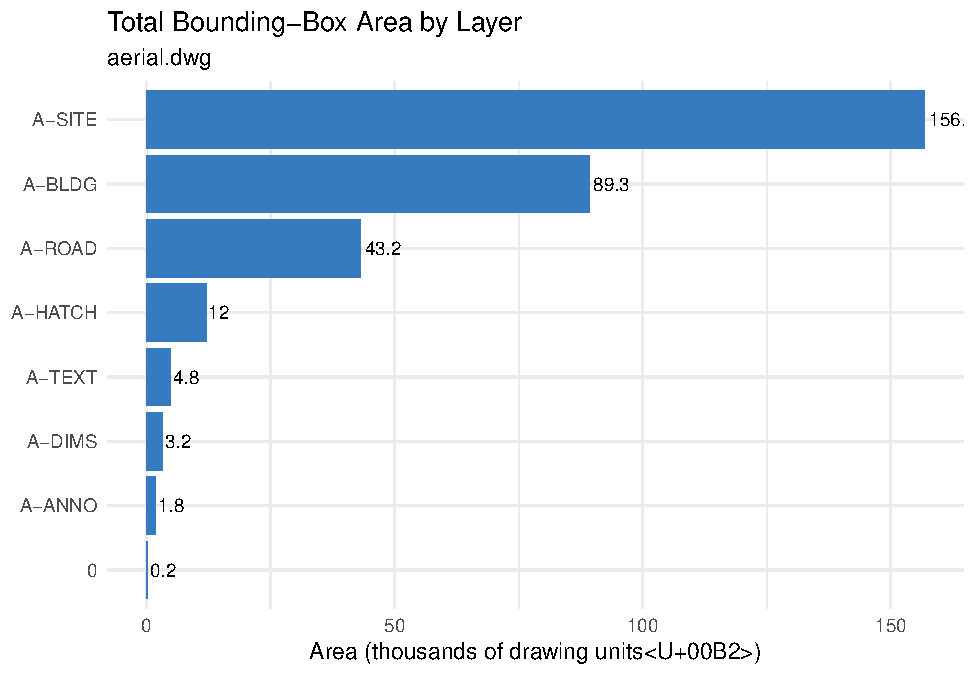
\includegraphics[keepaspectratio]{layer-analysis_files/figure-pdf/unnamed-chunk-9-1.pdf}}

\section{Objects per Layer --- Dot
Plot}\label{objects-per-layer-dot-plot}

A dot plot works better than a bar chart when you want to compare both
count \emph{and} area simultaneously:

\begin{Shaded}
\begin{Highlighting}[]
\FunctionTok{ggplot}\NormalTok{(layer\_summary, }\FunctionTok{aes}\NormalTok{(}\AttributeTok{x =}\NormalTok{ n\_objects, }\AttributeTok{y =} \FunctionTok{reorder}\NormalTok{(layer, n\_objects))) }\SpecialCharTok{+}
  \FunctionTok{geom\_point}\NormalTok{(}\FunctionTok{aes}\NormalTok{(}\AttributeTok{size =}\NormalTok{ total\_area }\SpecialCharTok{/} \DecValTok{1000}\NormalTok{), }\AttributeTok{colour =} \StringTok{"\#367ABF"}\NormalTok{, }\AttributeTok{alpha =} \FloatTok{0.8}\NormalTok{) }\SpecialCharTok{+}
  \FunctionTok{geom\_text}\NormalTok{(}\FunctionTok{aes}\NormalTok{(}\AttributeTok{label =}\NormalTok{ n\_objects), }\AttributeTok{hjust =} \SpecialCharTok{{-}}\FloatTok{0.8}\NormalTok{, }\AttributeTok{size =} \DecValTok{3}\NormalTok{) }\SpecialCharTok{+}
  \FunctionTok{scale\_size\_continuous}\NormalTok{(}\AttributeTok{name =} \StringTok{"Total area}\SpecialCharTok{\textbackslash{}n}\StringTok{(thousands of units²)"}\NormalTok{,}
                        \AttributeTok{range =} \FunctionTok{c}\NormalTok{(}\DecValTok{2}\NormalTok{, }\DecValTok{10}\NormalTok{)) }\SpecialCharTok{+}
  \FunctionTok{labs}\NormalTok{(}\AttributeTok{title =} \StringTok{"Objects per Layer"}\NormalTok{,}
       \AttributeTok{subtitle =} \StringTok{"Point size proportional to total bounding{-}box area"}\NormalTok{,}
       \AttributeTok{x =} \StringTok{"Object count"}\NormalTok{, }\AttributeTok{y =} \ConstantTok{NULL}\NormalTok{) }\SpecialCharTok{+}
  \FunctionTok{theme\_minimal}\NormalTok{()}
\end{Highlighting}
\end{Shaded}

\pandocbounded{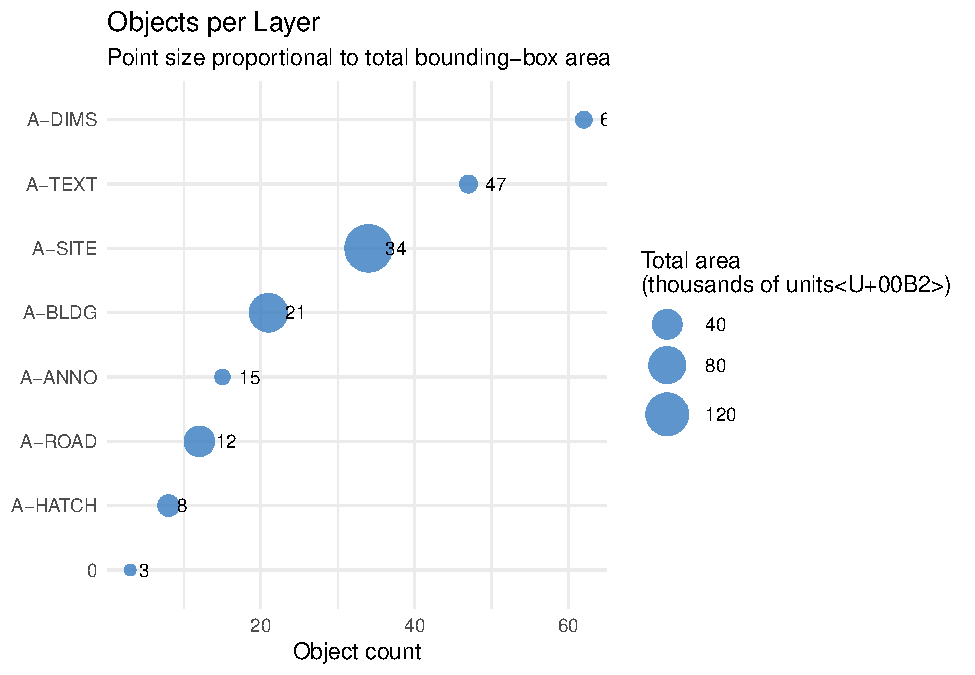
\includegraphics[keepaspectratio]{layer-analysis_files/figure-pdf/unnamed-chunk-10-1.pdf}}

The \texttt{props\_df} and \texttt{layer\_summary} objects carry forward
into \href{attribute-extraction.qmd}{Attribute Extraction} and
\href{cross-drawing-comparison.qmd}{Cross-Drawing Comparison}.

\chapter{Attribute Extraction}\label{attribute-extraction}

Layer names and bounding boxes are just the start. DWG files also carry
custom properties and block attributes, zone designations, construction
types, sheet numbers, column marks, that make the drawing data genuinely
useful for analysis. This chapter extracts those properties from the
\texttt{getData()} response and reshapes them into analysis-ready data
frames.

This chapter uses \texttt{collection} from
\hyperref[layer-structure-analysis]{Layer Structure Analysis}.

\section{Custom Properties}\label{custom-properties}

Custom properties appear under non-standard category names in
\texttt{obj\$properties}. The standard categories to exclude are
\texttt{"Layer\ and\ Material"}, \texttt{"Geometry"}, and
\texttt{"General"}:

\begin{Shaded}
\begin{Highlighting}[]
\FunctionTok{library}\NormalTok{(dplyr)}

\NormalTok{std\_cats }\OtherTok{\textless{}{-}} \FunctionTok{c}\NormalTok{(}\StringTok{"Layer and Material"}\NormalTok{, }\StringTok{"Geometry"}\NormalTok{, }\StringTok{"General"}\NormalTok{)}

\NormalTok{custom\_df }\OtherTok{\textless{}{-}} \FunctionTok{lapply}\NormalTok{(collection, }\ControlFlowTok{function}\NormalTok{(obj) \{}
\NormalTok{  props\_flat  }\OtherTok{\textless{}{-}} \FunctionTok{unlist}\NormalTok{(obj}\SpecialCharTok{$}\NormalTok{properties, }\AttributeTok{use.names =} \ConstantTok{TRUE}\NormalTok{)}
\NormalTok{  custom\_keys }\OtherTok{\textless{}{-}} \FunctionTok{names}\NormalTok{(props\_flat)[}
    \SpecialCharTok{!}\FunctionTok{grepl}\NormalTok{(}\FunctionTok{paste}\NormalTok{(std\_cats, }\AttributeTok{collapse =} \StringTok{"|"}\NormalTok{), }\FunctionTok{names}\NormalTok{(props\_flat))}
\NormalTok{  ]}
  \ControlFlowTok{if}\NormalTok{ (}\FunctionTok{length}\NormalTok{(custom\_keys) }\SpecialCharTok{==} \DecValTok{0}\NormalTok{) }\FunctionTok{return}\NormalTok{(}\ConstantTok{NULL}\NormalTok{)}
  \FunctionTok{data.frame}\NormalTok{(}\AttributeTok{objectid   =}\NormalTok{ obj}\SpecialCharTok{$}\NormalTok{objectid,}
             \AttributeTok{prop\_name  =}\NormalTok{ custom\_keys,}
             \AttributeTok{prop\_value =}\NormalTok{ props\_flat[custom\_keys],}
             \AttributeTok{stringsAsFactors =} \ConstantTok{FALSE}\NormalTok{)}
\NormalTok{\}) }\SpecialCharTok{|\textgreater{}} \FunctionTok{do.call}\NormalTok{(}\AttributeTok{what =}\NormalTok{ rbind)}

\FunctionTok{head}\NormalTok{(custom\_df)}
\CommentTok{\#\textgreater{}   objectid              prop\_name      prop\_value}
\CommentTok{\#\textgreater{} 1       42        Custom.Zone          Zone A}
\CommentTok{\#\textgreater{} 2       42 Custom.Construction.Type   RC Frame}
\CommentTok{\#\textgreater{} 3       42     Custom.Floor.Area          428.5}
\CommentTok{\#\textgreater{} 4       43        Custom.Zone          Zone B}
\end{Highlighting}
\end{Shaded}

\section{Block Attributes}\label{block-attributes}

Block inserts carry named attributes under
\texttt{obj\$properties\$Attributes}:

\begin{Shaded}
\begin{Highlighting}[]
\NormalTok{block\_df }\OtherTok{\textless{}{-}} \FunctionTok{lapply}\NormalTok{(collection, }\ControlFlowTok{function}\NormalTok{(obj) \{}
  \ControlFlowTok{if}\NormalTok{ (}\FunctionTok{is.null}\NormalTok{(obj}\SpecialCharTok{$}\NormalTok{properties}\SpecialCharTok{$}\NormalTok{Attributes)) }\FunctionTok{return}\NormalTok{(}\ConstantTok{NULL}\NormalTok{)}
\NormalTok{  attrs }\OtherTok{\textless{}{-}}\NormalTok{ obj}\SpecialCharTok{$}\NormalTok{properties}\SpecialCharTok{$}\NormalTok{Attributes}
  \FunctionTok{data.frame}\NormalTok{(}\AttributeTok{objectid   =}\NormalTok{ obj}\SpecialCharTok{$}\NormalTok{objectid,}
             \AttributeTok{block\_name =}\NormalTok{ obj}\SpecialCharTok{$}\NormalTok{name,}
             \AttributeTok{attr\_name  =} \FunctionTok{names}\NormalTok{(attrs),}
             \AttributeTok{attr\_value =} \FunctionTok{unlist}\NormalTok{(attrs),}
             \AttributeTok{stringsAsFactors =} \ConstantTok{FALSE}\NormalTok{)}
\NormalTok{\}) }\SpecialCharTok{|\textgreater{}} \FunctionTok{do.call}\NormalTok{(}\AttributeTok{what =}\NormalTok{ rbind)}

\FunctionTok{head}\NormalTok{(block\_df)}
\CommentTok{\#\textgreater{}   objectid  block\_name    attr\_name  attr\_value}
\CommentTok{\#\textgreater{} 1       88 TITLE{-}BLOCK   SHEET\_NO      A{-}001}
\CommentTok{\#\textgreater{} 2       88 TITLE{-}BLOCK   REVISION      Rev 3}
\CommentTok{\#\textgreater{} 3       89  COLUMN{-}TAG   MARK          C1}
\CommentTok{\#\textgreater{} 4       89  COLUMN{-}TAG   GRID          A/1}
\end{Highlighting}
\end{Shaded}

\section{Pivot to Wide Format}\label{pivot-to-wide-format}

Long-form property data is easy to filter but awkward to join.
\texttt{pivot\_wider()} gives you one column per property:

\begin{Shaded}
\begin{Highlighting}[]
\FunctionTok{library}\NormalTok{(tidyr)}

\NormalTok{custom\_wide }\OtherTok{\textless{}{-}}\NormalTok{ custom\_df }\SpecialCharTok{|\textgreater{}}
  \FunctionTok{mutate}\NormalTok{(}\AttributeTok{prop\_name =} \FunctionTok{sub}\NormalTok{(}\StringTok{"\^{}Custom}\SpecialCharTok{\textbackslash{}\textbackslash{}}\StringTok{."}\NormalTok{, }\StringTok{""}\NormalTok{, prop\_name)) }\SpecialCharTok{|\textgreater{}}
  \FunctionTok{pivot\_wider}\NormalTok{(}\AttributeTok{names\_from  =}\NormalTok{ prop\_name,}
              \AttributeTok{values\_from =}\NormalTok{ prop\_value)}

\FunctionTok{head}\NormalTok{(custom\_wide)}
\CommentTok{\#\textgreater{} \# A tibble: 3 × 4}
\CommentTok{\#\textgreater{}   objectid Zone   Construction.Type Floor.Area}
\CommentTok{\#\textgreater{}      \textless{}int\textgreater{} \textless{}chr\textgreater{}  \textless{}chr\textgreater{}             \textless{}chr\textgreater{}}
\CommentTok{\#\textgreater{} 1       42 Zone A RC Frame          428.5}
\CommentTok{\#\textgreater{} 2       43 Zone B Steel Frame       312.0}
\CommentTok{\#\textgreater{} 3       51 Zone A Masonry           198.3}
\end{Highlighting}
\end{Shaded}

\section{Join Attributes to Layer
Data}\label{join-attributes-to-layer-data}

Merge custom properties back onto the geometry data frame for combined
analysis:

\begin{Shaded}
\begin{Highlighting}[]
\NormalTok{enriched }\OtherTok{\textless{}{-}}\NormalTok{ props\_df }\SpecialCharTok{|\textgreater{}}
  \FunctionTok{left\_join}\NormalTok{(custom\_wide, }\AttributeTok{by =} \StringTok{"objectid"}\NormalTok{)}
\end{Highlighting}
\end{Shaded}

\section{Floor Area by Zone and Construction
Type}\label{floor-area-by-zone-and-construction-type}

\begin{Shaded}
\begin{Highlighting}[]
\NormalTok{zone\_summary }\OtherTok{\textless{}{-}}\NormalTok{ enriched }\SpecialCharTok{|\textgreater{}}
  \FunctionTok{filter}\NormalTok{(layer }\SpecialCharTok{==} \StringTok{"A{-}BLDG"}\NormalTok{, }\SpecialCharTok{!}\FunctionTok{is.na}\NormalTok{(Zone)) }\SpecialCharTok{|\textgreater{}}
  \FunctionTok{mutate}\NormalTok{(}\AttributeTok{floor\_area =} \FunctionTok{as.numeric}\NormalTok{(Floor.Area)) }\SpecialCharTok{|\textgreater{}}
  \FunctionTok{group\_by}\NormalTok{(Zone, Construction.Type) }\SpecialCharTok{|\textgreater{}}
  \FunctionTok{summarise}\NormalTok{(}\AttributeTok{total\_floor\_area =} \FunctionTok{sum}\NormalTok{(floor\_area, }\AttributeTok{na.rm =} \ConstantTok{TRUE}\NormalTok{),}
            \AttributeTok{n\_units          =} \FunctionTok{n}\NormalTok{(),}
            \AttributeTok{.groups          =} \StringTok{"drop"}\NormalTok{)}

\NormalTok{zone\_summary}
\CommentTok{\#\textgreater{} \# A tibble: 3 × 4}
\CommentTok{\#\textgreater{}   Zone   Construction.Type total\_floor\_area n\_units}
\CommentTok{\#\textgreater{} 1 Zone A Masonry                      198.3       1}
\CommentTok{\#\textgreater{} 2 Zone A RC Frame                     428.5       1}
\CommentTok{\#\textgreater{} 3 Zone B Steel Frame                  312.0       1}
\end{Highlighting}
\end{Shaded}

\section{Visualising Custom
Attributes}\label{visualising-custom-attributes}

A stacked bar chart of floor area by zone and construction type:

\begin{verbatim}
Warning: package 'ggplot2' was built under R version 4.4.3
\end{verbatim}

\begin{Shaded}
\begin{Highlighting}[]
\FunctionTok{ggplot}\NormalTok{(zone\_summary,}
       \FunctionTok{aes}\NormalTok{(}\AttributeTok{x =}\NormalTok{ Zone, }\AttributeTok{y =}\NormalTok{ total\_floor\_area, }\AttributeTok{fill =}\NormalTok{ Construction.Type)) }\SpecialCharTok{+}
  \FunctionTok{geom\_col}\NormalTok{(}\AttributeTok{position =} \StringTok{"stack"}\NormalTok{) }\SpecialCharTok{+}
  \FunctionTok{geom\_text}\NormalTok{(}\FunctionTok{aes}\NormalTok{(}\AttributeTok{label =} \FunctionTok{paste0}\NormalTok{(}\FunctionTok{round}\NormalTok{(total\_floor\_area, }\DecValTok{0}\NormalTok{), }\StringTok{" m²"}\NormalTok{)),}
            \AttributeTok{position =} \FunctionTok{position\_stack}\NormalTok{(}\AttributeTok{vjust =} \FloatTok{0.5}\NormalTok{),}
            \AttributeTok{colour =} \StringTok{"white"}\NormalTok{, }\AttributeTok{size =} \FloatTok{3.5}\NormalTok{) }\SpecialCharTok{+}
  \FunctionTok{scale\_fill\_manual}\NormalTok{(}\AttributeTok{values =} \FunctionTok{c}\NormalTok{(}\StringTok{"\#367ABF"}\NormalTok{, }\StringTok{"\#4CAF50"}\NormalTok{, }\StringTok{"\#F4A261"}\NormalTok{)) }\SpecialCharTok{+}
  \FunctionTok{labs}\NormalTok{(}\AttributeTok{title =} \StringTok{"Floor Area by Zone and Construction Type"}\NormalTok{,}
       \AttributeTok{subtitle =} \StringTok{"Extracted from block attributes — aerial.dwg"}\NormalTok{,}
       \AttributeTok{x =} \ConstantTok{NULL}\NormalTok{, }\AttributeTok{y =} \StringTok{"Floor area (m²)"}\NormalTok{, }\AttributeTok{fill =} \StringTok{"Construction type"}\NormalTok{) }\SpecialCharTok{+}
  \FunctionTok{theme\_minimal}\NormalTok{()}
\end{Highlighting}
\end{Shaded}

\pandocbounded{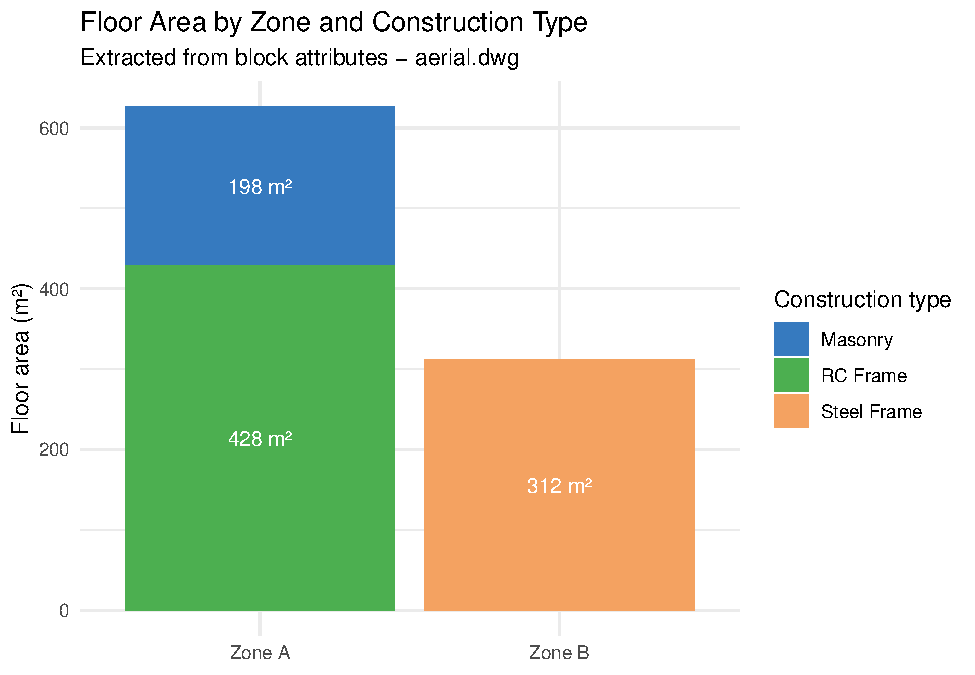
\includegraphics[keepaspectratio]{attribute-extraction_files/figure-pdf/unnamed-chunk-7-1.pdf}}

\section{Export}\label{export}

Write the enriched data frame to CSV for handover or further processing:

\begin{Shaded}
\begin{Highlighting}[]
\FunctionTok{write.csv}\NormalTok{(enriched, }\AttributeTok{file =} \StringTok{"drawing\_attributes.csv"}\NormalTok{, }\AttributeTok{row.names =} \ConstantTok{FALSE}\NormalTok{)}
\end{Highlighting}
\end{Shaded}

\chapter{Cross-Drawing Comparison}\label{cross-drawing-comparison}

Got a drawing set? Multiple revisions? Discipline packages from
different consultants? This chapter shows how to compare their layer
structures systematically, what layers were added, what was removed, and
where the object counts changed most between versions.

\section{Upload Multiple Drawings}\label{upload-multiple-drawings}

Upload each DWG to the same OSS bucket (see
\hyperref[data-management]{Data Management}):

\begin{Shaded}
\begin{Highlighting}[]
\FunctionTok{library}\NormalTok{(AutoDeskR)}
\FunctionTok{library}\NormalTok{(dplyr)}

\NormalTok{resp    }\OtherTok{\textless{}{-}} \FunctionTok{getToken}\NormalTok{(}\AttributeTok{id     =} \FunctionTok{Sys.getenv}\NormalTok{(}\StringTok{"client\_id"}\NormalTok{),}
                    \AttributeTok{secret =} \FunctionTok{Sys.getenv}\NormalTok{(}\StringTok{"client\_secret"}\NormalTok{),}
                    \AttributeTok{scope  =} \StringTok{"data:read data:write"}\NormalTok{)}
\NormalTok{myToken }\OtherTok{\textless{}{-}}\NormalTok{ resp}\SpecialCharTok{$}\NormalTok{content}\SpecialCharTok{$}\NormalTok{access\_token}

\NormalTok{dwg\_files }\OtherTok{\textless{}{-}} \FunctionTok{c}\NormalTok{(}\StringTok{"floor\_plan\_v1.dwg"}\NormalTok{, }\StringTok{"floor\_plan\_v2.dwg"}\NormalTok{, }\StringTok{"site\_plan.dwg"}\NormalTok{)}

\NormalTok{urns }\OtherTok{\textless{}{-}} \FunctionTok{sapply}\NormalTok{(dwg\_files, }\ControlFlowTok{function}\NormalTok{(f) \{}
\NormalTok{  resp }\OtherTok{\textless{}{-}} \FunctionTok{uploadFile}\NormalTok{(}\AttributeTok{file   =}\NormalTok{ f,}
                     \AttributeTok{token  =}\NormalTok{ myToken,}
                     \AttributeTok{bucket =} \FunctionTok{Sys.getenv}\NormalTok{(}\StringTok{"bucket"}\NormalTok{))}
\NormalTok{  resp}\SpecialCharTok{$}\NormalTok{content}\SpecialCharTok{$}\NormalTok{objectId}
\NormalTok{\})}
\end{Highlighting}
\end{Shaded}

\section{Extract Layer Sets}\label{extract-layer-sets}

A helper function wraps the translate → poll → tree chain for one file
and returns its layer names:

\begin{Shaded}
\begin{Highlighting}[]
\NormalTok{get\_layers }\OtherTok{\textless{}{-}} \ControlFlowTok{function}\NormalTok{(urn, token) \{}
\NormalTok{  enc\_urn }\OtherTok{\textless{}{-}}\NormalTok{ jsonlite}\SpecialCharTok{::}\FunctionTok{base64\_enc}\NormalTok{(urn)}
  \FunctionTok{translateSvf}\NormalTok{(}\AttributeTok{urn =}\NormalTok{ enc\_urn, }\AttributeTok{token =}\NormalTok{ token)}
  \ControlFlowTok{repeat}\NormalTok{ \{}
    \ControlFlowTok{if}\NormalTok{ (}\FunctionTok{checkFile}\NormalTok{(}\AttributeTok{urn =}\NormalTok{ enc\_urn, }\AttributeTok{token =}\NormalTok{ token)}\SpecialCharTok{$}\NormalTok{content}\SpecialCharTok{$}\NormalTok{status }\SpecialCharTok{==} \StringTok{"success"}\NormalTok{) }\ControlFlowTok{break}
    \FunctionTok{Sys.sleep}\NormalTok{(}\DecValTok{5}\NormalTok{)}
\NormalTok{  \}}
\NormalTok{  meta }\OtherTok{\textless{}{-}} \FunctionTok{getMetadata}\NormalTok{(}\AttributeTok{urn =}\NormalTok{ enc\_urn, }\AttributeTok{token =}\NormalTok{ token)}
\NormalTok{  guid }\OtherTok{\textless{}{-}}\NormalTok{ meta}\SpecialCharTok{$}\NormalTok{content}\SpecialCharTok{$}\NormalTok{data}\SpecialCharTok{$}\NormalTok{metadata[[}\DecValTok{1}\NormalTok{]]}\SpecialCharTok{$}\NormalTok{guid}
\NormalTok{  tree }\OtherTok{\textless{}{-}} \FunctionTok{getObjectTree}\NormalTok{(}\AttributeTok{guid =}\NormalTok{ guid, }\AttributeTok{urn =}\NormalTok{ enc\_urn, }\AttributeTok{token =}\NormalTok{ token)}
\NormalTok{  root }\OtherTok{\textless{}{-}}\NormalTok{ tree}\SpecialCharTok{$}\NormalTok{content}\SpecialCharTok{$}\NormalTok{data}\SpecialCharTok{$}\NormalTok{objects[[}\DecValTok{1}\NormalTok{]]}
\NormalTok{  layer\_nodes }\OtherTok{\textless{}{-}} \FunctionTok{Filter}\NormalTok{(}\ControlFlowTok{function}\NormalTok{(n) }\FunctionTok{grepl}\NormalTok{(}\StringTok{"\^{}Layer:"}\NormalTok{, n}\SpecialCharTok{$}\NormalTok{name), root}\SpecialCharTok{$}\NormalTok{objects)}
  \FunctionTok{sub}\NormalTok{(}\StringTok{"\^{}Layer: "}\NormalTok{, }\StringTok{""}\NormalTok{, }\FunctionTok{vapply}\NormalTok{(layer\_nodes, }\StringTok{\textasciigrave{}}\AttributeTok{[[}\StringTok{\textasciigrave{}}\NormalTok{, }\FunctionTok{character}\NormalTok{(}\DecValTok{1}\NormalTok{), }\StringTok{"name"}\NormalTok{))}
\NormalTok{\}}

\NormalTok{layer\_sets }\OtherTok{\textless{}{-}} \FunctionTok{lapply}\NormalTok{(urns, get\_layers, }\AttributeTok{token =}\NormalTok{ myToken)}
\end{Highlighting}
\end{Shaded}

\section{What Changed?}\label{what-changed}

\texttt{setdiff()} pinpoints additions and removals:

\begin{Shaded}
\begin{Highlighting}[]
\NormalTok{added   }\OtherTok{\textless{}{-}} \FunctionTok{setdiff}\NormalTok{(layer\_sets[[}\StringTok{"floor\_plan\_v2.dwg"}\NormalTok{]],}
\NormalTok{                   layer\_sets[[}\StringTok{"floor\_plan\_v1.dwg"}\NormalTok{]])}
\NormalTok{removed }\OtherTok{\textless{}{-}} \FunctionTok{setdiff}\NormalTok{(layer\_sets[[}\StringTok{"floor\_plan\_v1.dwg"}\NormalTok{]],}
\NormalTok{                   layer\_sets[[}\StringTok{"floor\_plan\_v2.dwg"}\NormalTok{]])}

\FunctionTok{cat}\NormalTok{(}\StringTok{"Added:  "}\NormalTok{, }\FunctionTok{paste}\NormalTok{(added,   }\AttributeTok{collapse =} \StringTok{", "}\NormalTok{), }\StringTok{"}\SpecialCharTok{\textbackslash{}n}\StringTok{"}\NormalTok{)}
\CommentTok{\#\textgreater{} Added:   A{-}FURN{-}NEW, A{-}ELEC{-}EV}
\FunctionTok{cat}\NormalTok{(}\StringTok{"Removed:"}\NormalTok{, }\FunctionTok{paste}\NormalTok{(removed, }\AttributeTok{collapse =} \StringTok{", "}\NormalTok{), }\StringTok{"}\SpecialCharTok{\textbackslash{}n}\StringTok{"}\NormalTok{)}
\CommentTok{\#\textgreater{} Removed: A{-}TEMP{-}SITE}
\end{Highlighting}
\end{Shaded}

\section{Presence Matrix}\label{presence-matrix}

Build a tidy data frame showing which layers appear in which drawings:

\begin{Shaded}
\begin{Highlighting}[]
\NormalTok{all\_layers   }\OtherTok{\textless{}{-}} \FunctionTok{unique}\NormalTok{(}\FunctionTok{unlist}\NormalTok{(layer\_sets))}
\NormalTok{presence\_df  }\OtherTok{\textless{}{-}} \FunctionTok{data.frame}\NormalTok{(}\AttributeTok{layer =}\NormalTok{ all\_layers)}

\ControlFlowTok{for}\NormalTok{ (nm }\ControlFlowTok{in} \FunctionTok{names}\NormalTok{(layer\_sets)) \{}
\NormalTok{  presence\_df[[nm]] }\OtherTok{\textless{}{-}}\NormalTok{ all\_layers }\SpecialCharTok{\%in\%}\NormalTok{ layer\_sets[[nm]]}
\NormalTok{\}}
\end{Highlighting}
\end{Shaded}

\section{Layer Presence Heatmap}\label{layer-presence-heatmap}

A heatmap is the clearest way to show presence/absence across many
drawings:

\begin{verbatim}
Warning: package 'ggplot2' was built under R version 4.4.3
\end{verbatim}

\begin{Shaded}
\begin{Highlighting}[]
\FunctionTok{ggplot}\NormalTok{(heat\_df, }\FunctionTok{aes}\NormalTok{(}\AttributeTok{x =}\NormalTok{ drawing, }\AttributeTok{y =}\NormalTok{ layer, }\AttributeTok{fill =}\NormalTok{ present)) }\SpecialCharTok{+}
  \FunctionTok{geom\_tile}\NormalTok{(}\AttributeTok{colour =} \StringTok{"white"}\NormalTok{, }\AttributeTok{linewidth =} \FloatTok{0.5}\NormalTok{) }\SpecialCharTok{+}
  \FunctionTok{scale\_fill\_manual}\NormalTok{(}\AttributeTok{values  =} \FunctionTok{c}\NormalTok{(}\StringTok{"FALSE"} \OtherTok{=} \StringTok{"\#f0f0f0"}\NormalTok{, }\StringTok{"TRUE"} \OtherTok{=} \StringTok{"\#367ABF"}\NormalTok{),}
                    \AttributeTok{labels  =} \FunctionTok{c}\NormalTok{(}\StringTok{"FALSE"} \OtherTok{=} \StringTok{"Absent"}\NormalTok{, }\StringTok{"TRUE"} \OtherTok{=} \StringTok{"Present"}\NormalTok{)) }\SpecialCharTok{+}
  \FunctionTok{labs}\NormalTok{(}\AttributeTok{title =} \StringTok{"Layer Presence Across Drawings"}\NormalTok{,}
       \AttributeTok{x =} \ConstantTok{NULL}\NormalTok{, }\AttributeTok{y =} \ConstantTok{NULL}\NormalTok{, }\AttributeTok{fill =} \ConstantTok{NULL}\NormalTok{) }\SpecialCharTok{+}
  \FunctionTok{theme\_minimal}\NormalTok{() }\SpecialCharTok{+}
  \FunctionTok{theme}\NormalTok{(}\AttributeTok{axis.text.x =} \FunctionTok{element\_text}\NormalTok{(}\AttributeTok{angle =} \DecValTok{30}\NormalTok{, }\AttributeTok{hjust =} \DecValTok{1}\NormalTok{),}
        \AttributeTok{legend.position =} \StringTok{"bottom"}\NormalTok{)}
\end{Highlighting}
\end{Shaded}

\pandocbounded{
\includegraphics[keepaspectratio]{cross-drawing-comparison_files/figure-pdf/unnamed-chunk-6-1.pdf}}

\section{Object Count Changes}\label{object-count-changes}

Go one level deeper: not just whether a layer exists, but how many
objects it contains and how that changed:

\begin{Shaded}
\begin{Highlighting}[]
\NormalTok{get\_layer\_counts }\OtherTok{\textless{}{-}} \ControlFlowTok{function}\NormalTok{(urn, token) \{}
\NormalTok{  enc\_urn   }\OtherTok{\textless{}{-}}\NormalTok{ jsonlite}\SpecialCharTok{::}\FunctionTok{base64\_enc}\NormalTok{(urn)}
\NormalTok{  meta      }\OtherTok{\textless{}{-}} \FunctionTok{getMetadata}\NormalTok{(}\AttributeTok{urn =}\NormalTok{ enc\_urn, }\AttributeTok{token =}\NormalTok{ token)}
\NormalTok{  guid      }\OtherTok{\textless{}{-}}\NormalTok{ meta}\SpecialCharTok{$}\NormalTok{content}\SpecialCharTok{$}\NormalTok{data}\SpecialCharTok{$}\NormalTok{metadata[[}\DecValTok{1}\NormalTok{]]}\SpecialCharTok{$}\NormalTok{guid}
\NormalTok{  data\_resp }\OtherTok{\textless{}{-}} \FunctionTok{getData}\NormalTok{(}\AttributeTok{guid =}\NormalTok{ guid, }\AttributeTok{urn =}\NormalTok{ enc\_urn, }\AttributeTok{token =}\NormalTok{ token)}
  \FunctionTok{lapply}\NormalTok{(data\_resp}\SpecialCharTok{$}\NormalTok{content}\SpecialCharTok{$}\NormalTok{data}\SpecialCharTok{$}\NormalTok{collection, }\ControlFlowTok{function}\NormalTok{(obj) \{}
    \FunctionTok{data.frame}\NormalTok{(}\AttributeTok{layer =}\NormalTok{ obj}\SpecialCharTok{$}\NormalTok{properties[[}\StringTok{"Layer and Material"}\NormalTok{]][[}\StringTok{"Layer"}\NormalTok{]],}
               \AttributeTok{stringsAsFactors =} \ConstantTok{FALSE}\NormalTok{)}
\NormalTok{  \}) }\SpecialCharTok{|\textgreater{}} \FunctionTok{do.call}\NormalTok{(}\AttributeTok{what =}\NormalTok{ rbind) }\SpecialCharTok{|\textgreater{}} \FunctionTok{count}\NormalTok{(layer, }\AttributeTok{name =} \StringTok{"n\_objects"}\NormalTok{)}
\NormalTok{\}}

\NormalTok{counts\_v1 }\OtherTok{\textless{}{-}} \FunctionTok{get\_layer\_counts}\NormalTok{(urns[[}\StringTok{"floor\_plan\_v1.dwg"}\NormalTok{]], myToken)}
\NormalTok{counts\_v2 }\OtherTok{\textless{}{-}} \FunctionTok{get\_layer\_counts}\NormalTok{(urns[[}\StringTok{"floor\_plan\_v2.dwg"}\NormalTok{]], myToken)}

\NormalTok{comparison }\OtherTok{\textless{}{-}} \FunctionTok{full\_join}\NormalTok{(counts\_v1, counts\_v2, }\AttributeTok{by =} \StringTok{"layer"}\NormalTok{,}
                        \AttributeTok{suffix =} \FunctionTok{c}\NormalTok{(}\StringTok{"\_v1"}\NormalTok{, }\StringTok{"\_v2"}\NormalTok{)) }\SpecialCharTok{|\textgreater{}}
  \FunctionTok{mutate}\NormalTok{(}\AttributeTok{change =} \FunctionTok{replace\_na}\NormalTok{(n\_objects\_v2, }\DecValTok{0}\NormalTok{L) }\SpecialCharTok{{-}}
                  \FunctionTok{replace\_na}\NormalTok{(n\_objects\_v1, }\DecValTok{0}\NormalTok{L)) }\SpecialCharTok{|\textgreater{}}
  \FunctionTok{arrange}\NormalTok{(}\FunctionTok{desc}\NormalTok{(}\FunctionTok{abs}\NormalTok{(change)))}

\NormalTok{comparison}
\CommentTok{\#\textgreater{}         layer n\_objects\_v1 n\_objects\_v2 change}
\CommentTok{\#\textgreater{} 1      A{-}FURN           NA           34     34}
\CommentTok{\#\textgreater{} 2  A{-}FURN{-}NEW           NA           12     12}
\CommentTok{\#\textgreater{} 3    A{-}ELEC             8           18     10}
\CommentTok{\#\textgreater{} 4    A{-}BLDG            21           23      2}
\CommentTok{\#\textgreater{} 5  A{-}TEMP{-}SITE         5           NA     {-}5}
\end{Highlighting}
\end{Shaded}

\section{Change Waterfall Chart}\label{change-waterfall-chart}

A waterfall chart makes the direction and magnitude of each change
immediately readable:

\begin{Shaded}
\begin{Highlighting}[]
\FunctionTok{ggplot}\NormalTok{(comparison,}
       \FunctionTok{aes}\NormalTok{(}\AttributeTok{x =} \FunctionTok{reorder}\NormalTok{(layer, change),}
           \AttributeTok{y =}\NormalTok{ change,}
           \AttributeTok{fill =}\NormalTok{ change }\SpecialCharTok{\textgreater{}} \DecValTok{0}\NormalTok{)) }\SpecialCharTok{+}
  \FunctionTok{geom\_col}\NormalTok{(}\AttributeTok{show.legend =} \ConstantTok{FALSE}\NormalTok{) }\SpecialCharTok{+}
  \FunctionTok{geom\_hline}\NormalTok{(}\AttributeTok{yintercept =} \DecValTok{0}\NormalTok{, }\AttributeTok{linewidth =} \FloatTok{0.4}\NormalTok{) }\SpecialCharTok{+}
  \FunctionTok{scale\_fill\_manual}\NormalTok{(}\AttributeTok{values =} \FunctionTok{c}\NormalTok{(}\StringTok{"TRUE"} \OtherTok{=} \StringTok{"\#4CAF50"}\NormalTok{, }\StringTok{"FALSE"} \OtherTok{=} \StringTok{"\#d6604d"}\NormalTok{)) }\SpecialCharTok{+}
  \FunctionTok{coord\_flip}\NormalTok{() }\SpecialCharTok{+}
  \FunctionTok{labs}\NormalTok{(}\AttributeTok{title =} \StringTok{"Object Count Changes: v1 → v2"}\NormalTok{,}
       \AttributeTok{subtitle =} \StringTok{"Green = added objects, red = removed"}\NormalTok{,}
       \AttributeTok{x =} \ConstantTok{NULL}\NormalTok{, }\AttributeTok{y =} \StringTok{"Change in object count"}\NormalTok{) }\SpecialCharTok{+}
  \FunctionTok{theme\_minimal}\NormalTok{()}
\end{Highlighting}
\end{Shaded}

\pandocbounded{
\includegraphics[keepaspectratio]{cross-drawing-comparison_files/figure-pdf/unnamed-chunk-9-1.pdf}}

\chapter{Automated Drawing Reports}\label{automated-drawing-reports}

You've got the layer summary, the attribute data, the charts. Now let's
wrap it all into a polished, reproducible report that regenerates
automatically whenever a new DWG lands in the bucket. This chapter
combines \texttt{gt} (Iannone et al. 2024) tables with Quarto's
parameterised rendering to produce professional HTML reports with one
function call.

\section{A gt Summary Table}\label{a-gt-summary-table}

\texttt{gt} turns a data frame into a presentation-ready table in a few
chained calls. The \texttt{layer\_summary} from
\hyperref[layer-structure-analysis]{Layer Structure Analysis} is a
natural fit:

\begin{Shaded}
\begin{Highlighting}[]
\FunctionTok{library}\NormalTok{(gt)}

\NormalTok{layer\_summary }\SpecialCharTok{|\textgreater{}}
  \FunctionTok{gt}\NormalTok{() }\SpecialCharTok{|\textgreater{}}
  \FunctionTok{tab\_header}\NormalTok{(}
    \AttributeTok{title    =} \StringTok{"Drawing Layer Summary"}\NormalTok{,}
    \AttributeTok{subtitle =} \StringTok{"aerial.dwg — AutoDeskR extraction"}
\NormalTok{  ) }\SpecialCharTok{|\textgreater{}}
  \FunctionTok{cols\_label}\NormalTok{(}
    \AttributeTok{layer      =} \StringTok{"Layer"}\NormalTok{,}
    \AttributeTok{n\_objects  =} \StringTok{"Objects"}\NormalTok{,}
    \AttributeTok{total\_area =} \StringTok{"Total Area"}\NormalTok{,}
    \AttributeTok{mean\_area  =} \StringTok{"Mean Area"}
\NormalTok{  ) }\SpecialCharTok{|\textgreater{}}
  \FunctionTok{fmt\_number}\NormalTok{(}\AttributeTok{columns =} \FunctionTok{c}\NormalTok{(total\_area, mean\_area), }\AttributeTok{decimals =} \DecValTok{1}\NormalTok{) }\SpecialCharTok{|\textgreater{}}
  \FunctionTok{tab\_style}\NormalTok{(}
    \AttributeTok{style     =} \FunctionTok{cell\_fill}\NormalTok{(}\AttributeTok{color =} \StringTok{"\#EBF3FB"}\NormalTok{),}
    \AttributeTok{locations =} \FunctionTok{cells\_column\_labels}\NormalTok{()}
\NormalTok{  ) }\SpecialCharTok{|\textgreater{}}
  \FunctionTok{tab\_source\_note}\NormalTok{(}
    \AttributeTok{source\_note =} \FunctionTok{paste}\NormalTok{(}\StringTok{"Extracted"}\NormalTok{, }\FunctionTok{Sys.Date}\NormalTok{(), }\StringTok{"via AutoDeskR v0.4.0"}\NormalTok{)}
\NormalTok{  ) }\SpecialCharTok{|\textgreater{}}
  \FunctionTok{tab\_options}\NormalTok{(}\AttributeTok{table.font.size =} \StringTok{"small"}\NormalTok{)}
\end{Highlighting}
\end{Shaded}

\section{Parameterised Reports}\label{parameterised-reports}

A parameterised Quarto document accepts different inputs at render time,
making it reusable for any DWG without editing the source file. Add a
\texttt{params} block to the YAML:

\begin{Shaded}
\begin{Highlighting}[]
\PreprocessorTok{{-}{-}{-}}
\FunctionTok{title}\KeywordTok{:}\AttributeTok{ }\StringTok{"Drawing Report"}
\FunctionTok{format}\KeywordTok{:}\AttributeTok{ html}
\FunctionTok{params}\KeywordTok{:}
\AttributeTok{  }\FunctionTok{urn}\KeywordTok{:}\AttributeTok{ }\StringTok{"YOUR\_URN\_HERE"}
\AttributeTok{  }\FunctionTok{drawing\_name}\KeywordTok{:}\AttributeTok{ }\StringTok{"aerial.dwg"}
\PreprocessorTok{{-}{-}{-}}
\end{Highlighting}
\end{Shaded}

Access the parameters inside the document:

\begin{Shaded}
\begin{Highlighting}[]
\NormalTok{urn          }\OtherTok{\textless{}{-}}\NormalTok{ params}\SpecialCharTok{$}\NormalTok{urn}
\NormalTok{drawing\_name }\OtherTok{\textless{}{-}}\NormalTok{ params}\SpecialCharTok{$}\NormalTok{drawing\_name}
\end{Highlighting}
\end{Shaded}

Use \texttt{drawing\_name} in headings so each rendered report is
self-labelled:

\begin{Shaded}
\begin{Highlighting}[]
\FunctionTok{cat}\NormalTok{(}\StringTok{"\#\# Layer Summary:"}\NormalTok{, drawing\_name, }\StringTok{"}\SpecialCharTok{\textbackslash{}n}\StringTok{"}\NormalTok{)}
\end{Highlighting}
\end{Shaded}

\section{Render Programmatically}\label{render-programmatically}

\texttt{quarto::quarto\_render()} renders the parameterised template to
a named output file. Loop over your drawing list to generate a report
for each one:

\begin{Shaded}
\begin{Highlighting}[]
\FunctionTok{library}\NormalTok{(quarto)}

\NormalTok{drawings }\OtherTok{\textless{}{-}} \FunctionTok{list}\NormalTok{(}
  \FunctionTok{list}\NormalTok{(}\AttributeTok{urn =}\NormalTok{ urns[[}\StringTok{"site\_plan.dwg"}\NormalTok{]],      }\AttributeTok{name =} \StringTok{"site\_plan"}\NormalTok{),}
  \FunctionTok{list}\NormalTok{(}\AttributeTok{urn =}\NormalTok{ urns[[}\StringTok{"floor\_plan\_v2.dwg"}\NormalTok{]], }\AttributeTok{name =} \StringTok{"floor\_plan\_v2"}\NormalTok{)}
\NormalTok{)}

\ControlFlowTok{for}\NormalTok{ (dwg }\ControlFlowTok{in}\NormalTok{ drawings) \{}
  \FunctionTok{quarto\_render}\NormalTok{(}
    \AttributeTok{input          =} \StringTok{"drawing{-}reports.qmd"}\NormalTok{,}
    \AttributeTok{output\_file    =} \FunctionTok{paste0}\NormalTok{(}\StringTok{"report\_"}\NormalTok{, dwg}\SpecialCharTok{$}\NormalTok{name, }\StringTok{".html"}\NormalTok{),}
    \AttributeTok{execute\_params =} \FunctionTok{list}\NormalTok{(}
      \AttributeTok{urn          =}\NormalTok{ dwg}\SpecialCharTok{$}\NormalTok{urn,}
      \AttributeTok{drawing\_name =} \FunctionTok{paste0}\NormalTok{(dwg}\SpecialCharTok{$}\NormalTok{name, }\StringTok{".dwg"}\NormalTok{)}
\NormalTok{    )}
\NormalTok{  )}
  \FunctionTok{cat}\NormalTok{(}\StringTok{"Generated: report\_"}\NormalTok{, dwg}\SpecialCharTok{$}\NormalTok{name, }\StringTok{".html}\SpecialCharTok{\textbackslash{}n}\StringTok{"}\NormalTok{, }\AttributeTok{sep =} \StringTok{""}\NormalTok{)}
\NormalTok{\}}
\CommentTok{\#\textgreater{} Generated: report\_site\_plan.html}
\CommentTok{\#\textgreater{} Generated: report\_floor\_plan\_v2.html}
\end{Highlighting}
\end{Shaded}

\section{Scheduling Reports}\label{scheduling-reports}

Keep reports fresh automatically by triggering \texttt{quarto\_render()}
on a schedule.

\textbf{GitHub Actions} --- run on a cron or whenever DWGs are pushed:

\begin{Shaded}
\begin{Highlighting}[]
\CommentTok{\# .github/workflows/drawing{-}report.yml}
\FunctionTok{on}\KeywordTok{:}
\AttributeTok{  }\FunctionTok{schedule}\KeywordTok{:}
\AttributeTok{    }\KeywordTok{{-}}\AttributeTok{ }\FunctionTok{cron}\KeywordTok{:}\AttributeTok{ }\StringTok{"0 6 * * 1"}\CommentTok{   \# every Monday at 06:00 UTC}
\AttributeTok{  }\FunctionTok{push}\KeywordTok{:}
\AttributeTok{    }\FunctionTok{paths}\KeywordTok{:}\AttributeTok{ }\KeywordTok{[}\StringTok{"dwg{-}files/**"}\KeywordTok{]}

\FunctionTok{jobs}\KeywordTok{:}
\AttributeTok{  }\FunctionTok{render}\KeywordTok{:}
\AttributeTok{    }\FunctionTok{runs{-}on}\KeywordTok{:}\AttributeTok{ ubuntu{-}latest}
\AttributeTok{    }\FunctionTok{steps}\KeywordTok{:}
\AttributeTok{      }\KeywordTok{{-}}\AttributeTok{ }\FunctionTok{uses}\KeywordTok{:}\AttributeTok{ actions/checkout@v4}
\AttributeTok{      }\KeywordTok{{-}}\AttributeTok{ }\FunctionTok{uses}\KeywordTok{:}\AttributeTok{ r{-}lib/actions/setup{-}r@v2}
\AttributeTok{      }\KeywordTok{{-}}\AttributeTok{ }\FunctionTok{run}\KeywordTok{:}\AttributeTok{ Rscript {-}e \textquotesingle{}quarto::quarto\_render("drawing{-}reports.qmd")\textquotesingle{}}
\end{Highlighting}
\end{Shaded}

\textbf{cronR (local)} --- schedule from a local R session:

\begin{Shaded}
\begin{Highlighting}[]
\FunctionTok{library}\NormalTok{(cronR)}
\NormalTok{cmd }\OtherTok{\textless{}{-}} \FunctionTok{cron\_rscript}\NormalTok{(}\StringTok{"render\_reports.R"}\NormalTok{)}
\FunctionTok{cron\_add}\NormalTok{(}\AttributeTok{command     =}\NormalTok{ cmd,}
         \AttributeTok{frequency   =} \StringTok{"weekly"}\NormalTok{,}
         \AttributeTok{at          =} \StringTok{"06:00"}\NormalTok{,}
         \AttributeTok{id          =} \StringTok{"drawing\_report"}\NormalTok{,}
         \AttributeTok{description =} \StringTok{"Weekly DWG report"}\NormalTok{)}
\end{Highlighting}
\end{Shaded}

\begin{tcolorbox}[enhanced jigsaw, titlerule=0mm, colback=white, colframe=quarto-callout-tip-color-frame, bottomtitle=1mm, bottomrule=.15mm, coltitle=black, arc=.35mm, left=2mm, title=\textcolor{quarto-callout-tip-color}{\faLightbulb}\hspace{0.5em}{Tip}, colbacktitle=quarto-callout-tip-color!10!white, toptitle=1mm, breakable, toprule=.15mm, rightrule=.15mm, leftrule=.75mm, opacitybacktitle=0.6, opacityback=0]

Store credentials (\texttt{client\_id}, \texttt{client\_secret}, bucket
name) as GitHub Actions secrets or in
\texttt{\textasciitilde{}/.Renviron} on the local machine. Never
hardcode them in the report source file. Your future self will thank
you.

\end{tcolorbox}

\part{Digital Twins}

\chapter{AutoDesk Tandem Overview}\label{autodesk-tandem-overview}

A BIM model is a snapshot of a building at design time. A
\textbf{digital twin} takes that same model and connects it to the
building's live operational data --- temperature sensors, occupancy
counters, energy meters --- so you can see what's actually happening
inside, not just what was drawn. AutoDesk Tandem is APS's platform for
building and querying digital twins.

This chapter introduces Tandem concepts and shows how to talk to the
Tandem REST API directly from R using \texttt{httr2} (Wickham 2024) and
a standard APS token from \texttt{getToken()}. See (Autodesk, Inc. 2024)
for the full API reference.

The relationship between a BIM model and a Tandem twin looks like this:

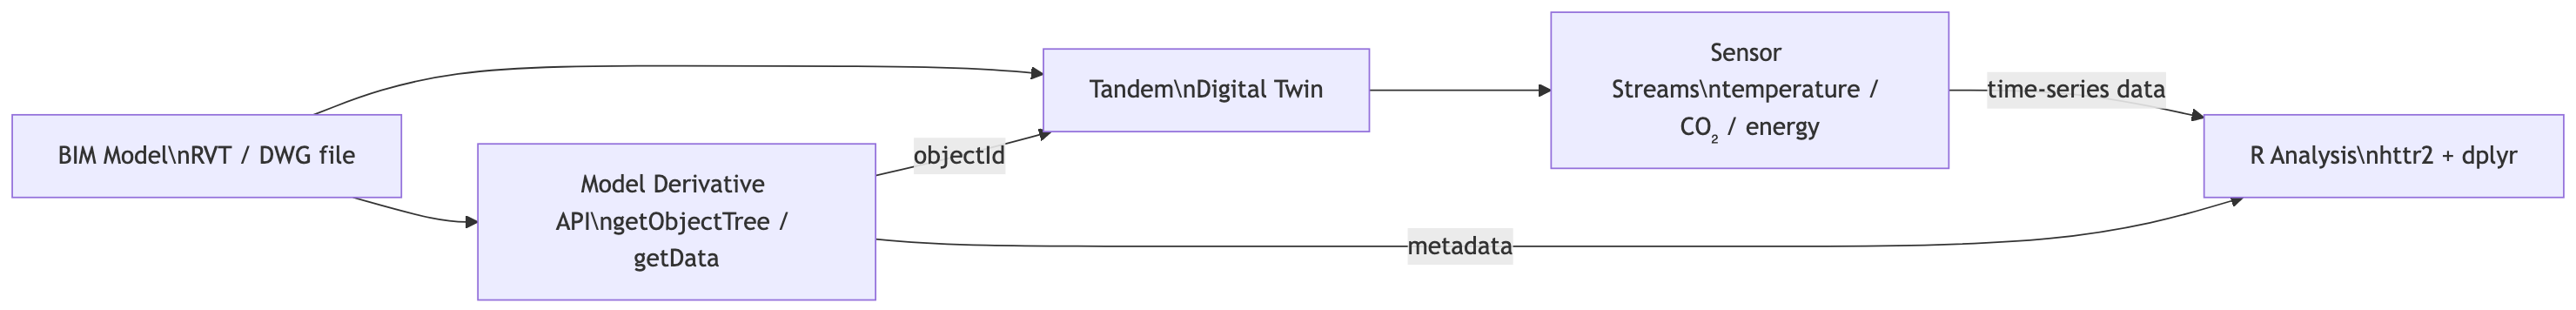
\includegraphics[width=17.54in,height=2.13in]{tandem-overview_files/figure-latex/mermaid-figure-1.png}

\begin{tcolorbox}[enhanced jigsaw, titlerule=0mm, colback=white, colframe=quarto-callout-tip-color-frame, bottomtitle=1mm, bottomrule=.15mm, coltitle=black, arc=.35mm, left=2mm, title=\textcolor{quarto-callout-tip-color}{\faLightbulb}\hspace{0.5em}{Tip}, colbacktitle=quarto-callout-tip-color!10!white, toptitle=1mm, breakable, toprule=.15mm, rightrule=.15mm, leftrule=.75mm, opacitybacktitle=0.6, opacityback=0]

Tandem requires an active \textbf{AutoDesk Tandem subscription} in
addition to an APS app registration. Authentication uses the same OAuth
Bearer token as the rest of this book --- no extra credential setup
needed.

\end{tcolorbox}

\section{Twin vs.~BIM Model}\label{twin-vs.-bim-model}

\begin{longtable}[]{@{}
  >{\raggedright\arraybackslash}p{(\linewidth - 4\tabcolsep) * \real{0.3333}}
  >{\raggedright\arraybackslash}p{(\linewidth - 4\tabcolsep) * \real{0.3333}}
  >{\raggedright\arraybackslash}p{(\linewidth - 4\tabcolsep) * \real{0.3333}}@{}}
\toprule\noalign{}
\begin{minipage}[b]{\linewidth}\raggedright
\end{minipage} & \begin{minipage}[b]{\linewidth}\raggedright
BIM Model
\end{minipage} & \begin{minipage}[b]{\linewidth}\raggedright
Digital Twin
\end{minipage} \\
\midrule\noalign{}
\endhead
\bottomrule\noalign{}
\endlastfoot
Primary data & Geometry + properties & Geometry + live sensor streams \\
Update frequency & Per design revision & Continuous / real-time \\
Primary use & Design \& construction & Operations \& maintenance \\
APS API & Model Derivative & Tandem REST \\
R entry point & \texttt{getObjectTree()}, \texttt{getData()} &
\texttt{httr2::request()} \\
\end{longtable}

\section{Authentication}\label{authentication-1}

The Tandem API accepts the same Bearer token as all other APS services:

\begin{Shaded}
\begin{Highlighting}[]
\FunctionTok{library}\NormalTok{(AutoDeskR)}
\FunctionTok{library}\NormalTok{(httr2)}

\NormalTok{resp    }\OtherTok{\textless{}{-}} \FunctionTok{getToken}\NormalTok{(}\AttributeTok{id     =} \FunctionTok{Sys.getenv}\NormalTok{(}\StringTok{"client\_id"}\NormalTok{),}
                    \AttributeTok{secret =} \FunctionTok{Sys.getenv}\NormalTok{(}\StringTok{"client\_secret"}\NormalTok{),}
                    \AttributeTok{scope  =} \StringTok{"data:read"}\NormalTok{)}
\NormalTok{myToken }\OtherTok{\textless{}{-}}\NormalTok{ resp}\SpecialCharTok{$}\NormalTok{content}\SpecialCharTok{$}\NormalTok{access\_token}
\end{Highlighting}
\end{Shaded}

\section{Listing Facilities}\label{listing-facilities}

A \emph{facility} in Tandem is the digital twin of a building or site
--- the top-level container for model data and sensor streams. List all
facilities your token can access:

\begin{Shaded}
\begin{Highlighting}[]
\NormalTok{facilities\_resp }\OtherTok{\textless{}{-}} \FunctionTok{request}\NormalTok{(}\StringTok{"https://tandem.autodesk.com/api/v1/groups"}\NormalTok{) }\SpecialCharTok{|\textgreater{}}
  \FunctionTok{req\_auth\_bearer\_token}\NormalTok{(myToken) }\SpecialCharTok{|\textgreater{}}
  \FunctionTok{req\_perform}\NormalTok{()}

\NormalTok{facilities }\OtherTok{\textless{}{-}} \FunctionTok{resp\_body\_json}\NormalTok{(facilities\_resp)}

\NormalTok{facilities\_df }\OtherTok{\textless{}{-}} \FunctionTok{lapply}\NormalTok{(facilities, }\ControlFlowTok{function}\NormalTok{(f) \{}
  \FunctionTok{data.frame}\NormalTok{(}\AttributeTok{id =}\NormalTok{ f}\SpecialCharTok{$}\NormalTok{id, }\AttributeTok{name =}\NormalTok{ f}\SpecialCharTok{$}\NormalTok{name, }\AttributeTok{stringsAsFactors =} \ConstantTok{FALSE}\NormalTok{)}
\NormalTok{\}) }\SpecialCharTok{|\textgreater{}} \FunctionTok{do.call}\NormalTok{(}\AttributeTok{what =}\NormalTok{ rbind)}

\NormalTok{facilities\_df}
\CommentTok{\#\textgreater{}                                     id               name}
\CommentTok{\#\textgreater{} 1  urn:adsk.dtdm:facility.abc123def456  Office Block A}
\CommentTok{\#\textgreater{} 2  urn:adsk.dtdm:facility.xyz789uvw012  Warehouse Site B}
\end{Highlighting}
\end{Shaded}

\section{Facility Details}\label{facility-details}

\begin{Shaded}
\begin{Highlighting}[]
\NormalTok{facilityId }\OtherTok{\textless{}{-}} \StringTok{"urn:adsk.dtdm:facility.abc123def456"}

\NormalTok{facility\_resp }\OtherTok{\textless{}{-}} \FunctionTok{request}\NormalTok{(}
  \FunctionTok{paste0}\NormalTok{(}\StringTok{"https://tandem.autodesk.com/api/v1/twins/"}\NormalTok{, facilityId)}
\NormalTok{) }\SpecialCharTok{|\textgreater{}}
  \FunctionTok{req\_auth\_bearer\_token}\NormalTok{(myToken) }\SpecialCharTok{|\textgreater{}}
  \FunctionTok{req\_perform}\NormalTok{()}

\NormalTok{facility }\OtherTok{\textless{}{-}} \FunctionTok{resp\_body\_json}\NormalTok{(facility\_resp)}
\FunctionTok{cat}\NormalTok{(}\StringTok{"Name:        "}\NormalTok{, facility}\SpecialCharTok{$}\NormalTok{displayName, }\StringTok{"}\SpecialCharTok{\textbackslash{}n}\StringTok{"}\NormalTok{)}
\CommentTok{\#\textgreater{} Name:         Office Block A}
\FunctionTok{cat}\NormalTok{(}\StringTok{"Created:     "}\NormalTok{, facility}\SpecialCharTok{$}\NormalTok{createTime, }\StringTok{"}\SpecialCharTok{\textbackslash{}n}\StringTok{"}\NormalTok{)}
\CommentTok{\#\textgreater{} Created:      2025{-}11{-}04T09:22:14Z}
\FunctionTok{cat}\NormalTok{(}\StringTok{"Linked URNs:"}\NormalTok{, }\FunctionTok{length}\NormalTok{(facility}\SpecialCharTok{$}\NormalTok{links), }\StringTok{"}\SpecialCharTok{\textbackslash{}n}\StringTok{"}\NormalTok{)}
\CommentTok{\#\textgreater{} Linked URNs:  2}
\end{Highlighting}
\end{Shaded}

\texttt{facility\$links} contains the APS Model Derivative URNs of the
BIM models embedded in this twin --- the same URNs you'd pass to
\texttt{getObjectTree()} or \texttt{getData()}, which is what makes the
\texttt{objectId} the key that links the two worlds together.

\section{Looking Up an Element}\label{looking-up-an-element}

Any \texttt{objectId} from \texttt{getData()} can be looked up in Tandem
to find the corresponding physical element and its classification:

\begin{Shaded}
\begin{Highlighting}[]
\NormalTok{element\_resp }\OtherTok{\textless{}{-}} \FunctionTok{request}\NormalTok{(}
  \FunctionTok{paste0}\NormalTok{(}\StringTok{"https://tandem.autodesk.com/api/v1/twins/"}\NormalTok{,}
\NormalTok{         facilityId, }\StringTok{"/elements/"}\NormalTok{, }\DecValTok{42}\NormalTok{L)   }\CommentTok{\# objectId 42}
\NormalTok{) }\SpecialCharTok{|\textgreater{}}
  \FunctionTok{req\_auth\_bearer\_token}\NormalTok{(myToken) }\SpecialCharTok{|\textgreater{}}
  \FunctionTok{req\_perform}\NormalTok{()}

\NormalTok{element }\OtherTok{\textless{}{-}} \FunctionTok{resp\_body\_json}\NormalTok{(element\_resp)}
\FunctionTok{cat}\NormalTok{(}\StringTok{"Name:          "}\NormalTok{, element}\SpecialCharTok{$}\NormalTok{displayName, }\StringTok{"}\SpecialCharTok{\textbackslash{}n}\StringTok{"}\NormalTok{)}
\CommentTok{\#\textgreater{} Name:           Level 2 HVAC Unit}
\FunctionTok{cat}\NormalTok{(}\StringTok{"Classification:"}\NormalTok{, element}\SpecialCharTok{$}\NormalTok{classification, }\StringTok{"}\SpecialCharTok{\textbackslash{}n}\StringTok{"}\NormalTok{)}
\CommentTok{\#\textgreater{} Classification: MEP:HVAC:Air Handling Unit}
\end{Highlighting}
\end{Shaded}

The \href{sensor-streams.qmd}{Linking Sensor Streams} chapter shows how
to pull time-series readings for elements like this one.

\chapter{Linking Sensor Streams}\label{linking-sensor-streams}

Each element in a Tandem facility can have sensor streams attached to it
--- named time-series channels that report temperature, CO₂, occupancy,
energy consumption, or whatever the building management system sends.
Because streams are keyed to the same \texttt{objectId} that
\texttt{getObjectTree()} and \texttt{getData()} use, joining live sensor
data to BIM metadata is just a regular table join.

This chapter uses the facility set up in
\hyperref[autodesk-tandem-overview]{AutoDesk Tandem Overview}.

\section{Listing Streams for a
Facility}\label{listing-streams-for-a-facility}

\begin{Shaded}
\begin{Highlighting}[]
\FunctionTok{library}\NormalTok{(AutoDeskR)}
\FunctionTok{library}\NormalTok{(httr2)}
\FunctionTok{library}\NormalTok{(dplyr)}

\NormalTok{resp       }\OtherTok{\textless{}{-}} \FunctionTok{getToken}\NormalTok{(}\AttributeTok{id     =} \FunctionTok{Sys.getenv}\NormalTok{(}\StringTok{"client\_id"}\NormalTok{),}
                       \AttributeTok{secret =} \FunctionTok{Sys.getenv}\NormalTok{(}\StringTok{"client\_secret"}\NormalTok{),}
                       \AttributeTok{scope  =} \StringTok{"data:read"}\NormalTok{)}
\NormalTok{myToken    }\OtherTok{\textless{}{-}}\NormalTok{ resp}\SpecialCharTok{$}\NormalTok{content}\SpecialCharTok{$}\NormalTok{access\_token}
\NormalTok{facilityId }\OtherTok{\textless{}{-}} \StringTok{"urn:adsk.dtdm:facility.abc123def456"}

\NormalTok{streams\_resp }\OtherTok{\textless{}{-}} \FunctionTok{request}\NormalTok{(}
  \FunctionTok{paste0}\NormalTok{(}\StringTok{"https://tandem.autodesk.com/api/v1/twins/"}\NormalTok{, facilityId, }\StringTok{"/streams"}\NormalTok{)}
\NormalTok{) }\SpecialCharTok{|\textgreater{}}
  \FunctionTok{req\_auth\_bearer\_token}\NormalTok{(myToken) }\SpecialCharTok{|\textgreater{}}
  \FunctionTok{req\_perform}\NormalTok{()}

\NormalTok{streams }\OtherTok{\textless{}{-}} \FunctionTok{resp\_body\_json}\NormalTok{(streams\_resp)}

\NormalTok{streams\_df }\OtherTok{\textless{}{-}} \FunctionTok{lapply}\NormalTok{(streams, }\ControlFlowTok{function}\NormalTok{(s) \{}
  \FunctionTok{data.frame}\NormalTok{(}\AttributeTok{stream\_id    =}\NormalTok{ s}\SpecialCharTok{$}\NormalTok{id,}
             \AttributeTok{display\_name =}\NormalTok{ s}\SpecialCharTok{$}\NormalTok{displayName,}
             \AttributeTok{element\_id   =}\NormalTok{ s}\SpecialCharTok{$}\NormalTok{elementId,   }\CommentTok{\# objectId of the attached model element}
             \AttributeTok{unit         =}\NormalTok{ s}\SpecialCharTok{$}\NormalTok{unit,}
             \AttributeTok{last\_reading =}\NormalTok{ s}\SpecialCharTok{$}\NormalTok{lastValue,}
             \AttributeTok{stringsAsFactors =} \ConstantTok{FALSE}\NormalTok{)}
\NormalTok{\}) }\SpecialCharTok{|\textgreater{}} \FunctionTok{do.call}\NormalTok{(}\AttributeTok{what =}\NormalTok{ rbind)}

\NormalTok{streams\_df}
\CommentTok{\#\textgreater{}            stream\_id    display\_name element\_id  unit last\_reading}
\CommentTok{\#\textgreater{} 1  strm:temp{-}hvac{-}l2  HVAC Temp L2          42    °C         22.4}
\CommentTok{\#\textgreater{} 2  strm:co2{-}office{-}3  CO₂ Office 3         108   ppm        623.0}
\CommentTok{\#\textgreater{} 3  strm:occ{-}lobby     Lobby Occupancy        15  pers         14.0}
\CommentTok{\#\textgreater{} 4  strm:energy{-}main   Main Energy          201   kWh       8412.5}
\end{Highlighting}
\end{Shaded}

\section{Fetching Time-Series
Readings}\label{fetching-time-series-readings}

Request a time window using ISO 8601 timestamps as query parameters:

\begin{Shaded}
\begin{Highlighting}[]
\NormalTok{streamId   }\OtherTok{\textless{}{-}} \StringTok{"strm:temp{-}hvac{-}l2"}
\NormalTok{end\_time   }\OtherTok{\textless{}{-}} \FunctionTok{Sys.time}\NormalTok{()}
\NormalTok{start\_time }\OtherTok{\textless{}{-}}\NormalTok{ end\_time }\SpecialCharTok{{-}} \DecValTok{86400}   \CommentTok{\# last 24 hours}

\NormalTok{readings\_resp }\OtherTok{\textless{}{-}} \FunctionTok{request}\NormalTok{(}
  \FunctionTok{paste0}\NormalTok{(}\StringTok{"https://tandem.autodesk.com/api/v1/twins/"}\NormalTok{,}
\NormalTok{         facilityId, }\StringTok{"/streams/"}\NormalTok{, streamId)}
\NormalTok{) }\SpecialCharTok{|\textgreater{}}
  \FunctionTok{req\_url\_query}\NormalTok{(}
    \AttributeTok{start =} \FunctionTok{format}\NormalTok{(start\_time, }\StringTok{"\%Y{-}\%m{-}\%dT\%H:\%M:\%SZ"}\NormalTok{, }\AttributeTok{tz =} \StringTok{"UTC"}\NormalTok{),}
    \AttributeTok{end   =} \FunctionTok{format}\NormalTok{(end\_time,   }\StringTok{"\%Y{-}\%m{-}\%dT\%H:\%M:\%SZ"}\NormalTok{, }\AttributeTok{tz =} \StringTok{"UTC"}\NormalTok{)}
\NormalTok{  ) }\SpecialCharTok{|\textgreater{}}
  \FunctionTok{req\_auth\_bearer\_token}\NormalTok{(myToken) }\SpecialCharTok{|\textgreater{}}
  \FunctionTok{req\_perform}\NormalTok{()}

\NormalTok{readings }\OtherTok{\textless{}{-}} \FunctionTok{resp\_body\_json}\NormalTok{(readings\_resp)}

\NormalTok{readings\_df }\OtherTok{\textless{}{-}} \FunctionTok{data.frame}\NormalTok{(}
  \AttributeTok{timestamp =} \FunctionTok{as.POSIXct}\NormalTok{(}\FunctionTok{vapply}\NormalTok{(readings}\SpecialCharTok{$}\NormalTok{values, }\StringTok{\textasciigrave{}}\AttributeTok{[[}\StringTok{\textasciigrave{}}\NormalTok{, }\FunctionTok{character}\NormalTok{(}\DecValTok{1}\NormalTok{), }\StringTok{"t"}\NormalTok{),}
                          \AttributeTok{format =} \StringTok{"\%Y{-}\%m{-}\%dT\%H:\%M:\%SZ"}\NormalTok{, }\AttributeTok{tz =} \StringTok{"UTC"}\NormalTok{),}
  \AttributeTok{value     =} \FunctionTok{vapply}\NormalTok{(readings}\SpecialCharTok{$}\NormalTok{values, }\StringTok{\textasciigrave{}}\AttributeTok{[[}\StringTok{\textasciigrave{}}\NormalTok{, }\FunctionTok{numeric}\NormalTok{(}\DecValTok{1}\NormalTok{), }\StringTok{"v"}\NormalTok{),}
  \AttributeTok{stringsAsFactors =} \ConstantTok{FALSE}
\NormalTok{)}

\FunctionTok{head}\NormalTok{(readings\_df)}
\CommentTok{\#\textgreater{}             timestamp value}
\CommentTok{\#\textgreater{} 1 2026{-}04{-}23 06:00:00  21.8}
\CommentTok{\#\textgreater{} 2 2026{-}04{-}23 06:15:00  22.1}
\CommentTok{\#\textgreater{} 3 2026{-}04{-}23 06:30:00  22.4}
\end{Highlighting}
\end{Shaded}

\section{Plotting Readings}\label{plotting-readings}

\begin{verbatim}
Warning: package 'ggplot2' was built under R version 4.4.3
\end{verbatim}

\begin{Shaded}
\begin{Highlighting}[]
\FunctionTok{ggplot}\NormalTok{(readings\_df, }\FunctionTok{aes}\NormalTok{(}\AttributeTok{x =}\NormalTok{ timestamp, }\AttributeTok{y =}\NormalTok{ value)) }\SpecialCharTok{+}
  \FunctionTok{geom\_line}\NormalTok{(}\AttributeTok{colour =} \StringTok{"\#367ABF"}\NormalTok{, }\AttributeTok{linewidth =} \FloatTok{0.8}\NormalTok{) }\SpecialCharTok{+}
  \FunctionTok{geom\_ribbon}\NormalTok{(}\FunctionTok{aes}\NormalTok{(}\AttributeTok{ymin =}\NormalTok{ value }\SpecialCharTok{{-}} \FloatTok{0.5}\NormalTok{, }\AttributeTok{ymax =}\NormalTok{ value }\SpecialCharTok{+} \FloatTok{0.5}\NormalTok{),}
              \AttributeTok{fill =} \StringTok{"\#367ABF"}\NormalTok{, }\AttributeTok{alpha =} \FloatTok{0.15}\NormalTok{) }\SpecialCharTok{+}
  \FunctionTok{labs}\NormalTok{(}\AttributeTok{title    =} \StringTok{"HVAC Temperature — Level 2"}\NormalTok{,}
       \AttributeTok{subtitle =} \StringTok{"Last 24 hours"}\NormalTok{,}
       \AttributeTok{x =} \ConstantTok{NULL}\NormalTok{, }\AttributeTok{y =} \StringTok{"Temperature (°C)"}\NormalTok{) }\SpecialCharTok{+}
  \FunctionTok{theme\_minimal}\NormalTok{()}
\end{Highlighting}
\end{Shaded}

\pandocbounded{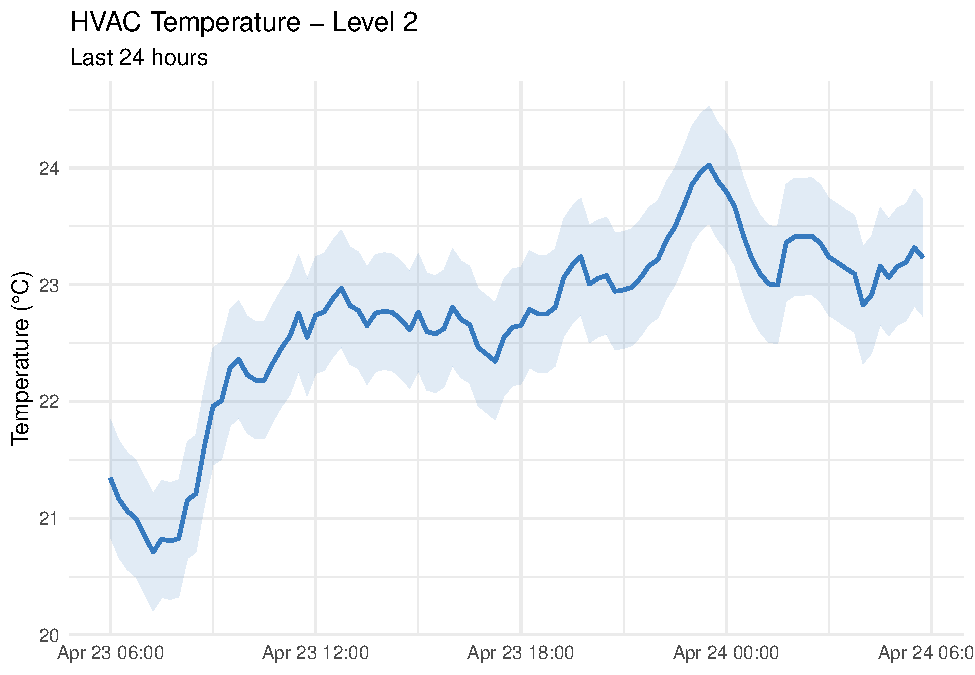
\includegraphics[keepaspectratio]{sensor-streams_files/figure-pdf/unnamed-chunk-4-1.pdf}}

\section{Joining Sensor Data to Model
Metadata}\label{joining-sensor-data-to-model-metadata}

\texttt{element\_id} in the streams response equals \texttt{objectid}
from \texttt{getData()}. A left join links live readings to layer,
classification, and any custom attributes:

\begin{Shaded}
\begin{Highlighting}[]
\CommentTok{\# props\_df from the Layer Structure Analysis chapter}

\NormalTok{joined }\OtherTok{\textless{}{-}}\NormalTok{ streams\_df }\SpecialCharTok{|\textgreater{}}
  \FunctionTok{inner\_join}\NormalTok{(props\_df }\SpecialCharTok{|\textgreater{}} \FunctionTok{select}\NormalTok{(objectid, layer),}
             \AttributeTok{by =} \FunctionTok{c}\NormalTok{(}\StringTok{"element\_id"} \OtherTok{=} \StringTok{"objectid"}\NormalTok{))}

\NormalTok{joined}
\CommentTok{\#\textgreater{}            stream\_id    display\_name element\_id   unit layer}
\CommentTok{\#\textgreater{} 1  strm:temp{-}hvac{-}l2  HVAC Temp L2          42    °C  M{-}HVAC}
\CommentTok{\#\textgreater{} 3  strm:occ{-}lobby     Lobby Occupancy        15  pers A{-}LBBY}
\end{Highlighting}
\end{Shaded}

\section{Fetching All Streams at
Once}\label{fetching-all-streams-at-once}

Loop over the stream list to build a single tidy data frame of all
readings:

\begin{Shaded}
\begin{Highlighting}[]
\NormalTok{all\_readings }\OtherTok{\textless{}{-}} \FunctionTok{lapply}\NormalTok{(streams\_df}\SpecialCharTok{$}\NormalTok{stream\_id, }\ControlFlowTok{function}\NormalTok{(sid) \{}
\NormalTok{  resp }\OtherTok{\textless{}{-}} \FunctionTok{request}\NormalTok{(}
    \FunctionTok{paste0}\NormalTok{(}\StringTok{"https://tandem.autodesk.com/api/v1/twins/"}\NormalTok{,}
\NormalTok{           facilityId, }\StringTok{"/streams/"}\NormalTok{, sid)}
\NormalTok{  ) }\SpecialCharTok{|\textgreater{}}
    \FunctionTok{req\_url\_query}\NormalTok{(}
      \AttributeTok{start =} \FunctionTok{format}\NormalTok{(start\_time, }\StringTok{"\%Y{-}\%m{-}\%dT\%H:\%M:\%SZ"}\NormalTok{, }\AttributeTok{tz =} \StringTok{"UTC"}\NormalTok{),}
      \AttributeTok{end   =} \FunctionTok{format}\NormalTok{(end\_time,   }\StringTok{"\%Y{-}\%m{-}\%dT\%H:\%M:\%SZ"}\NormalTok{, }\AttributeTok{tz =} \StringTok{"UTC"}\NormalTok{)}
\NormalTok{    ) }\SpecialCharTok{|\textgreater{}}
    \FunctionTok{req\_auth\_bearer\_token}\NormalTok{(myToken) }\SpecialCharTok{|\textgreater{}}
    \FunctionTok{req\_perform}\NormalTok{()}
\NormalTok{  readings }\OtherTok{\textless{}{-}} \FunctionTok{resp\_body\_json}\NormalTok{(resp)}
  \FunctionTok{data.frame}\NormalTok{(}\AttributeTok{stream\_id =}\NormalTok{ sid,}
             \AttributeTok{timestamp =} \FunctionTok{as.POSIXct}\NormalTok{(}
               \FunctionTok{vapply}\NormalTok{(readings}\SpecialCharTok{$}\NormalTok{values, }\StringTok{\textasciigrave{}}\AttributeTok{[[}\StringTok{\textasciigrave{}}\NormalTok{, }\FunctionTok{character}\NormalTok{(}\DecValTok{1}\NormalTok{), }\StringTok{"t"}\NormalTok{),}
               \AttributeTok{format =} \StringTok{"\%Y{-}\%m{-}\%dT\%H:\%M:\%SZ"}\NormalTok{, }\AttributeTok{tz =} \StringTok{"UTC"}\NormalTok{),}
             \AttributeTok{value     =} \FunctionTok{vapply}\NormalTok{(readings}\SpecialCharTok{$}\NormalTok{values, }\StringTok{\textasciigrave{}}\AttributeTok{[[}\StringTok{\textasciigrave{}}\NormalTok{, }\FunctionTok{numeric}\NormalTok{(}\DecValTok{1}\NormalTok{), }\StringTok{"v"}\NormalTok{),}
             \AttributeTok{stringsAsFactors =} \ConstantTok{FALSE}\NormalTok{)}
\NormalTok{\}) }\SpecialCharTok{|\textgreater{}} \FunctionTok{do.call}\NormalTok{(}\AttributeTok{what =}\NormalTok{ rbind)}

\CommentTok{\# Join display names and units}
\NormalTok{all\_readings }\OtherTok{\textless{}{-}}\NormalTok{ all\_readings }\SpecialCharTok{|\textgreater{}}
  \FunctionTok{left\_join}\NormalTok{(streams\_df }\SpecialCharTok{|\textgreater{}} \FunctionTok{select}\NormalTok{(stream\_id, display\_name, unit),}
            \AttributeTok{by =} \StringTok{"stream\_id"}\NormalTok{)}
\end{Highlighting}
\end{Shaded}

\section{Multi-Stream Overview Plot}\label{multi-stream-overview-plot}

\begin{Shaded}
\begin{Highlighting}[]
\FunctionTok{ggplot}\NormalTok{(all\_readings, }\FunctionTok{aes}\NormalTok{(}\AttributeTok{x =}\NormalTok{ timestamp, }\AttributeTok{y =}\NormalTok{ value, }\AttributeTok{colour =}\NormalTok{ display\_name)) }\SpecialCharTok{+}
  \FunctionTok{geom\_line}\NormalTok{(}\AttributeTok{linewidth =} \FloatTok{0.7}\NormalTok{) }\SpecialCharTok{+}
  \FunctionTok{facet\_wrap}\NormalTok{(}\SpecialCharTok{\textasciitilde{}} \FunctionTok{paste0}\NormalTok{(display\_name, }\StringTok{" ("}\NormalTok{, unit, }\StringTok{")"}\NormalTok{),}
             \AttributeTok{scales =} \StringTok{"free\_y"}\NormalTok{, }\AttributeTok{ncol =} \DecValTok{2}\NormalTok{) }\SpecialCharTok{+}
  \FunctionTok{labs}\NormalTok{(}\AttributeTok{title =} \StringTok{"All Sensor Streams — Last 24 Hours"}\NormalTok{,}
       \AttributeTok{x =} \ConstantTok{NULL}\NormalTok{, }\AttributeTok{y =} \ConstantTok{NULL}\NormalTok{) }\SpecialCharTok{+}
  \FunctionTok{theme\_minimal}\NormalTok{() }\SpecialCharTok{+}
  \FunctionTok{theme}\NormalTok{(}\AttributeTok{legend.position =} \StringTok{"none"}\NormalTok{)}
\end{Highlighting}
\end{Shaded}

\pandocbounded{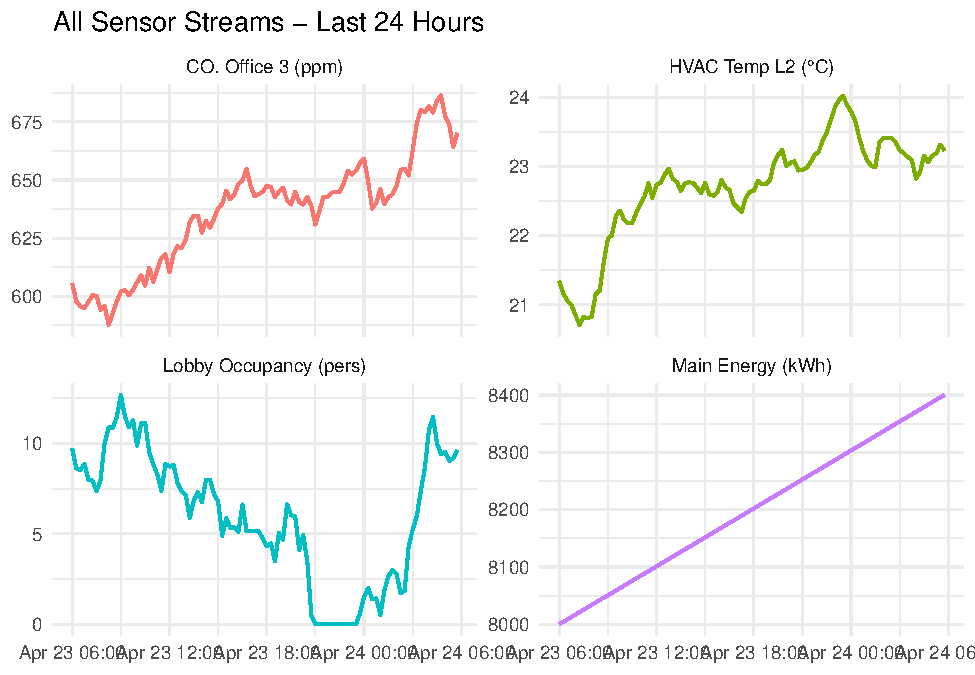
\includegraphics[keepaspectratio]{sensor-streams_files/figure-pdf/unnamed-chunk-8-1.pdf}}

The \texttt{all\_readings} data frame feeds directly into the
interactive Shiny dashboard in \href{live-dashboards.qmd}{Live
Dashboards}.

\chapter{Live Dashboards}\label{live-dashboards}

Here's where everything comes together: the 3D viewer from the
\hyperref[viewer]{Viewer} chapter on the left, live sensor charts from
\hyperref[linking-sensor-streams]{Linking Sensor Streams} on the right,
all in one Shiny app that refreshes automatically. This is what a
digital twin dashboard looks like in R.


\includegraphics[width=9.58in,height=2.06in]{live-dashboards_files/figure-latex/mermaid-figure-1.png}

\section{Required Packages}\label{required-packages}

\begin{Shaded}
\begin{Highlighting}[]
\FunctionTok{install.packages}\NormalTok{(}\FunctionTok{c}\NormalTok{(}\StringTok{"shiny"}\NormalTok{, }\StringTok{"dygraphs"}\NormalTok{, }\StringTok{"xts"}\NormalTok{, }\StringTok{"httr2"}\NormalTok{))}
\end{Highlighting}
\end{Shaded}

\section{Helper: Fetch Stream
Readings}\label{helper-fetch-stream-readings}

Define a reusable function that the Shiny server calls reactively:

\begin{Shaded}
\begin{Highlighting}[]
\FunctionTok{library}\NormalTok{(AutoDeskR)}
\FunctionTok{library}\NormalTok{(httr2)}
\FunctionTok{library}\NormalTok{(dygraphs)}
\FunctionTok{library}\NormalTok{(xts)}
\FunctionTok{library}\NormalTok{(shiny)}

\NormalTok{get\_stream\_readings }\OtherTok{\textless{}{-}} \ControlFlowTok{function}\NormalTok{(token, facility\_id, stream\_id, }\AttributeTok{hours\_back =} \DecValTok{24}\NormalTok{) \{}
\NormalTok{  end\_time   }\OtherTok{\textless{}{-}} \FunctionTok{Sys.time}\NormalTok{()}
\NormalTok{  start\_time }\OtherTok{\textless{}{-}}\NormalTok{ end\_time }\SpecialCharTok{{-}}\NormalTok{ hours\_back }\SpecialCharTok{*} \DecValTok{3600}
\NormalTok{  resp }\OtherTok{\textless{}{-}} \FunctionTok{request}\NormalTok{(}
    \FunctionTok{paste0}\NormalTok{(}\StringTok{"https://tandem.autodesk.com/api/v1/twins/"}\NormalTok{,}
\NormalTok{           facility\_id, }\StringTok{"/streams/"}\NormalTok{, stream\_id)}
\NormalTok{  ) }\SpecialCharTok{|\textgreater{}}
    \FunctionTok{req\_url\_query}\NormalTok{(}
      \AttributeTok{start =} \FunctionTok{format}\NormalTok{(start\_time, }\StringTok{"\%Y{-}\%m{-}\%dT\%H:\%M:\%SZ"}\NormalTok{, }\AttributeTok{tz =} \StringTok{"UTC"}\NormalTok{),}
      \AttributeTok{end   =} \FunctionTok{format}\NormalTok{(end\_time,   }\StringTok{"\%Y{-}\%m{-}\%dT\%H:\%M:\%SZ"}\NormalTok{, }\AttributeTok{tz =} \StringTok{"UTC"}\NormalTok{)}
\NormalTok{    ) }\SpecialCharTok{|\textgreater{}}
    \FunctionTok{req\_auth\_bearer\_token}\NormalTok{(token) }\SpecialCharTok{|\textgreater{}}
    \FunctionTok{req\_perform}\NormalTok{()}
\NormalTok{  readings }\OtherTok{\textless{}{-}} \FunctionTok{resp\_body\_json}\NormalTok{(resp)}
  \FunctionTok{data.frame}\NormalTok{(}
    \AttributeTok{timestamp =} \FunctionTok{as.POSIXct}\NormalTok{(}\FunctionTok{vapply}\NormalTok{(readings}\SpecialCharTok{$}\NormalTok{values, }\StringTok{\textasciigrave{}}\AttributeTok{[[}\StringTok{\textasciigrave{}}\NormalTok{, }\FunctionTok{character}\NormalTok{(}\DecValTok{1}\NormalTok{), }\StringTok{"t"}\NormalTok{),}
                            \AttributeTok{format =} \StringTok{"\%Y{-}\%m{-}\%dT\%H:\%M:\%SZ"}\NormalTok{, }\AttributeTok{tz =} \StringTok{"UTC"}\NormalTok{),}
    \AttributeTok{value     =} \FunctionTok{vapply}\NormalTok{(readings}\SpecialCharTok{$}\NormalTok{values, }\StringTok{\textasciigrave{}}\AttributeTok{[[}\StringTok{\textasciigrave{}}\NormalTok{, }\FunctionTok{numeric}\NormalTok{(}\DecValTok{1}\NormalTok{), }\StringTok{"v"}\NormalTok{),}
    \AttributeTok{stringsAsFactors =} \ConstantTok{FALSE}
\NormalTok{  )}
\NormalTok{\}}
\end{Highlighting}
\end{Shaded}

\section{App Startup}\label{app-startup}

Fetch the token and stream list once, before the UI and server are
defined:

\begin{Shaded}
\begin{Highlighting}[]
\NormalTok{myToken      }\OtherTok{\textless{}{-}} \FunctionTok{getToken}\NormalTok{(}\AttributeTok{id     =} \FunctionTok{Sys.getenv}\NormalTok{(}\StringTok{"client\_id"}\NormalTok{),}
                         \AttributeTok{secret =} \FunctionTok{Sys.getenv}\NormalTok{(}\StringTok{"client\_secret"}\NormalTok{),}
                         \AttributeTok{scope  =} \StringTok{"data:read"}\NormalTok{)}\SpecialCharTok{$}\NormalTok{content}\SpecialCharTok{$}\NormalTok{access\_token}
\NormalTok{myEncodedUrn }\OtherTok{\textless{}{-}}\NormalTok{ jsonlite}\SpecialCharTok{::}\FunctionTok{base64\_enc}\NormalTok{(}\FunctionTok{Sys.getenv}\NormalTok{(}\StringTok{"urn"}\NormalTok{))}
\NormalTok{facilityId   }\OtherTok{\textless{}{-}} \StringTok{"urn:adsk.dtdm:facility.abc123def456"}

\NormalTok{streams\_resp }\OtherTok{\textless{}{-}} \FunctionTok{request}\NormalTok{(}
  \FunctionTok{paste0}\NormalTok{(}\StringTok{"https://tandem.autodesk.com/api/v1/twins/"}\NormalTok{, facilityId, }\StringTok{"/streams"}\NormalTok{)}
\NormalTok{) }\SpecialCharTok{|\textgreater{}}
  \FunctionTok{req\_auth\_bearer\_token}\NormalTok{(myToken) }\SpecialCharTok{|\textgreater{}}
  \FunctionTok{req\_perform}\NormalTok{()}
\NormalTok{streams }\OtherTok{\textless{}{-}} \FunctionTok{resp\_body\_json}\NormalTok{(streams\_resp)}

\NormalTok{stream\_choices }\OtherTok{\textless{}{-}} \FunctionTok{setNames}\NormalTok{(}
  \FunctionTok{vapply}\NormalTok{(streams, }\StringTok{\textasciigrave{}}\AttributeTok{[[}\StringTok{\textasciigrave{}}\NormalTok{, }\FunctionTok{character}\NormalTok{(}\DecValTok{1}\NormalTok{), }\StringTok{"id"}\NormalTok{),}
  \FunctionTok{vapply}\NormalTok{(streams, }\StringTok{\textasciigrave{}}\AttributeTok{[[}\StringTok{\textasciigrave{}}\NormalTok{, }\FunctionTok{character}\NormalTok{(}\DecValTok{1}\NormalTok{), }\StringTok{"displayName"}\NormalTok{)}
\NormalTok{)}
\end{Highlighting}
\end{Shaded}

\section{UI Layout}\label{ui-layout}

Viewer on the left, controls and chart on the right:

\begin{Shaded}
\begin{Highlighting}[]
\NormalTok{ui }\OtherTok{\textless{}{-}} \FunctionTok{fluidPage}\NormalTok{(}
  \FunctionTok{titlePanel}\NormalTok{(}\StringTok{"Digital Twin Dashboard"}\NormalTok{),}
  \FunctionTok{fluidRow}\NormalTok{(}
    \FunctionTok{column}\NormalTok{(}\DecValTok{7}\NormalTok{,}
      \FunctionTok{viewer3D}\NormalTok{(}\AttributeTok{urn        =}\NormalTok{ myEncodedUrn,}
               \AttributeTok{token      =}\NormalTok{ myToken,}
               \AttributeTok{viewerType =} \StringTok{"headless"}\NormalTok{)}
\NormalTok{    ),}
    \FunctionTok{column}\NormalTok{(}\DecValTok{5}\NormalTok{,}
      \FunctionTok{selectInput}\NormalTok{(}\StringTok{"stream\_id"}\NormalTok{, }\StringTok{"Sensor stream:"}\NormalTok{,}
                  \AttributeTok{choices =}\NormalTok{ stream\_choices),}
      \FunctionTok{sliderInput}\NormalTok{(}\StringTok{"hours\_back"}\NormalTok{, }\StringTok{"Time window (hours):"}\NormalTok{,}
                  \AttributeTok{min =} \DecValTok{1}\NormalTok{, }\AttributeTok{max =} \DecValTok{168}\NormalTok{, }\AttributeTok{value =} \DecValTok{24}\NormalTok{, }\AttributeTok{step =} \DecValTok{1}\NormalTok{),}
      \FunctionTok{dygraphOutput}\NormalTok{(}\StringTok{"sensor\_plot"}\NormalTok{, }\AttributeTok{height =} \StringTok{"320px"}\NormalTok{),}
      \FunctionTok{tableOutput}\NormalTok{(}\StringTok{"stats\_table"}\NormalTok{)}
\NormalTok{    )}
\NormalTok{  )}
\NormalTok{)}
\end{Highlighting}
\end{Shaded}

\section{Server Logic}\label{server-logic}

A \texttt{reactiveTimer} polls Tandem every 60 seconds so the chart
stays current without the user having to refresh the page:

\begin{Shaded}
\begin{Highlighting}[]
\NormalTok{server }\OtherTok{\textless{}{-}} \ControlFlowTok{function}\NormalTok{(input, output, session) \{}

\NormalTok{  auto\_refresh }\OtherTok{\textless{}{-}} \FunctionTok{reactiveTimer}\NormalTok{(}\DecValTok{60000}\NormalTok{)   }\CommentTok{\# 60 seconds}

\NormalTok{  readings }\OtherTok{\textless{}{-}} \FunctionTok{reactive}\NormalTok{(\{}
    \FunctionTok{auto\_refresh}\NormalTok{()   }\CommentTok{\# re{-}run on the timer tick}
    \FunctionTok{get\_stream\_readings}\NormalTok{(}\AttributeTok{token       =}\NormalTok{ myToken,}
                        \AttributeTok{facility\_id =}\NormalTok{ facilityId,}
                        \AttributeTok{stream\_id   =}\NormalTok{ input}\SpecialCharTok{$}\NormalTok{stream\_id,}
                        \AttributeTok{hours\_back  =}\NormalTok{ input}\SpecialCharTok{$}\NormalTok{hours\_back)}
\NormalTok{  \})}

\NormalTok{  output}\SpecialCharTok{$}\NormalTok{sensor\_plot }\OtherTok{\textless{}{-}} \FunctionTok{renderDygraph}\NormalTok{(\{}
\NormalTok{    df   }\OtherTok{\textless{}{-}} \FunctionTok{readings}\NormalTok{()}
\NormalTok{    ts   }\OtherTok{\textless{}{-}} \FunctionTok{xts}\NormalTok{(df}\SpecialCharTok{$}\NormalTok{value, }\AttributeTok{order.by =}\NormalTok{ df}\SpecialCharTok{$}\NormalTok{timestamp)}
\NormalTok{    name }\OtherTok{\textless{}{-}} \FunctionTok{names}\NormalTok{(stream\_choices)[stream\_choices }\SpecialCharTok{==}\NormalTok{ input}\SpecialCharTok{$}\NormalTok{stream\_id]}
    \FunctionTok{dygraph}\NormalTok{(ts, }\AttributeTok{main =}\NormalTok{ name) }\SpecialCharTok{|\textgreater{}}
      \FunctionTok{dyRangeSelector}\NormalTok{() }\SpecialCharTok{|\textgreater{}}
      \FunctionTok{dyOptions}\NormalTok{(}\AttributeTok{fillGraph =} \ConstantTok{TRUE}\NormalTok{, }\AttributeTok{fillAlpha =} \FloatTok{0.15}\NormalTok{,}
                \AttributeTok{drawGrid  =} \ConstantTok{TRUE}\NormalTok{, }\AttributeTok{colors   =} \StringTok{"\#367ABF"}\NormalTok{) }\SpecialCharTok{|\textgreater{}}
      \FunctionTok{dyAxis}\NormalTok{(}\StringTok{"y"}\NormalTok{, }\AttributeTok{label =} \StringTok{"Value"}\NormalTok{)}
\NormalTok{  \})}

\NormalTok{  output}\SpecialCharTok{$}\NormalTok{stats\_table }\OtherTok{\textless{}{-}} \FunctionTok{renderTable}\NormalTok{(\{}
\NormalTok{    df }\OtherTok{\textless{}{-}} \FunctionTok{readings}\NormalTok{()}
    \FunctionTok{data.frame}\NormalTok{(}
      \AttributeTok{Metric =} \FunctionTok{c}\NormalTok{(}\StringTok{"Readings"}\NormalTok{, }\StringTok{"Mean"}\NormalTok{, }\StringTok{"Min"}\NormalTok{, }\StringTok{"Max"}\NormalTok{),}
      \AttributeTok{Value  =} \FunctionTok{c}\NormalTok{(}\FunctionTok{nrow}\NormalTok{(df),}
                 \FunctionTok{round}\NormalTok{(}\FunctionTok{mean}\NormalTok{(df}\SpecialCharTok{$}\NormalTok{value), }\DecValTok{2}\NormalTok{),}
                 \FunctionTok{round}\NormalTok{(}\FunctionTok{min}\NormalTok{(df}\SpecialCharTok{$}\NormalTok{value),  }\DecValTok{2}\NormalTok{),}
                 \FunctionTok{round}\NormalTok{(}\FunctionTok{max}\NormalTok{(df}\SpecialCharTok{$}\NormalTok{value),  }\DecValTok{2}\NormalTok{))}
\NormalTok{    )}
\NormalTok{  \}, }\AttributeTok{striped =} \ConstantTok{TRUE}\NormalTok{, }\AttributeTok{bordered =} \ConstantTok{TRUE}\NormalTok{, }\AttributeTok{align =} \StringTok{"lr"}\NormalTok{)}
\NormalTok{\}}

\FunctionTok{shinyApp}\NormalTok{(ui, server)}
\end{Highlighting}
\end{Shaded}

\begin{tcolorbox}[enhanced jigsaw, titlerule=0mm, colback=white, colframe=quarto-callout-warning-color-frame, bottomtitle=1mm, bottomrule=.15mm, coltitle=black, arc=.35mm, left=2mm, title=\textcolor{quarto-callout-warning-color}{\faExclamationTriangle}\hspace{0.5em}{Warning}, colbacktitle=quarto-callout-warning-color!10!white, toptitle=1mm, breakable, toprule=.15mm, rightrule=.15mm, leftrule=.75mm, opacitybacktitle=0.6, opacityback=0]

The Shiny server fetches Tandem data from R, not from the user's
browser, so CORS restrictions don't apply. The server process does need
outbound HTTPS access to \texttt{tandem.autodesk.com}, so check this if
you're deploying on a restricted corporate network.

\end{tcolorbox}

\section{Deploying to shinyapps.io}\label{deploying-to-shinyapps.io}

Keep credentials out of the app source. Pass them as server environment
variables at deploy time:

\begin{Shaded}
\begin{Highlighting}[]
\FunctionTok{library}\NormalTok{(rsconnect)}

\FunctionTok{deployApp}\NormalTok{(}
  \AttributeTok{appDir     =} \StringTok{"."}\NormalTok{,}
  \AttributeTok{appName    =} \StringTok{"twin{-}dashboard"}\NormalTok{,}
  \AttributeTok{appEnvVars =} \FunctionTok{list}\NormalTok{(}
    \AttributeTok{client\_id     =} \FunctionTok{Sys.getenv}\NormalTok{(}\StringTok{"client\_id"}\NormalTok{),}
    \AttributeTok{client\_secret =} \FunctionTok{Sys.getenv}\NormalTok{(}\StringTok{"client\_secret"}\NormalTok{),}
    \AttributeTok{urn           =} \FunctionTok{Sys.getenv}\NormalTok{(}\StringTok{"urn"}\NormalTok{)}
\NormalTok{  )}
\NormalTok{)}
\end{Highlighting}
\end{Shaded}

\begin{tcolorbox}[enhanced jigsaw, titlerule=0mm, colback=white, colframe=quarto-callout-tip-color-frame, bottomtitle=1mm, bottomrule=.15mm, coltitle=black, arc=.35mm, left=2mm, title=\textcolor{quarto-callout-tip-color}{\faLightbulb}\hspace{0.5em}{Tip}, colbacktitle=quarto-callout-tip-color!10!white, toptitle=1mm, breakable, toprule=.15mm, rightrule=.15mm, leftrule=.75mm, opacitybacktitle=0.6, opacityback=0]

The access token retrieved at startup expires after \textbf{1 hour}. For
a long-running production deployment, move \texttt{getToken()} inside
\texttt{get\_stream\_readings()} so a fresh token is requested on every
poll rather than once at startup.

\end{tcolorbox}

\part{AI Integration}

\chapter{MCP Server}\label{mcp-server}

AI assistants are increasingly useful not just for answering questions
but for \emph{doing things}, calling APIs, reading files, running
analyses. The Model Context Protocol (MCP) is the open standard that
makes that possible. It defines how an AI assistant discovers and calls
external tools during a conversation, in the same way a web browser
discovers and calls REST APIs.

AutoDeskR functions are exactly the kind of tools an AI agent would want
to call. ``Summarise the layers in this DWG.'' ``Translate this file and
give me the bounding box.'' ``Fetch the last 24 hours of HVAC sensor
readings.'' Each of those is a handful of AutoDeskR function calls, and
with an MCP server in front of them, an AI assistant can make those
calls itself, without you writing a single line of R.

This chapter shows how to expose AutoDeskR as an MCP server so that
Claude Desktop, VS Code Copilot, or any other MCP-compatible client can
query BIM models directly.

\section{Proposed Tools}\label{proposed-tools}

The table below maps ten useful MCP tools to their underlying AutoDeskR
functions. Each tool is a thin wrapper. It handles authentication, calls
the relevant function(s), and returns a structured JSON result.

\begin{longtable}[]{@{}
  >{\raggedright\arraybackslash}p{(\linewidth - 4\tabcolsep) * \real{0.3333}}
  >{\raggedright\arraybackslash}p{(\linewidth - 4\tabcolsep) * \real{0.3333}}
  >{\raggedright\arraybackslash}p{(\linewidth - 4\tabcolsep) * \real{0.3333}}@{}}
\toprule\noalign{}
\begin{minipage}[b]{\linewidth}\raggedright
MCP Tool
\end{minipage} & \begin{minipage}[b]{\linewidth}\raggedright
Wraps
\end{minipage} & \begin{minipage}[b]{\linewidth}\raggedright
Description
\end{minipage} \\
\midrule\noalign{}
\endhead
\bottomrule\noalign{}
\endlastfoot
\texttt{get\_token} & \texttt{getToken()} & Authenticate and return a
bearer token \\
\texttt{upload\_file} & \texttt{makeBucket()} + \texttt{uploadFile()} &
Create a bucket and upload a local file \\
\texttt{translate\_file} & \texttt{translateObj()} /
\texttt{translateSvf()} + \texttt{checkFile()} & Translate a file and
poll until complete \\
\texttt{get\_layer\_summary} & \texttt{translateSvf()} +
\texttt{getData()} & Layer-level object count and area for a DWG \\
\texttt{get\_object\_tree} & \texttt{getObjectTree()} & Model hierarchy
as a JSON tree \\
\texttt{get\_metadata} & \texttt{getMetadata()} & List available
metadata GUIDs for a translated model \\
\texttt{download\_mesh} & \texttt{getOutputUrn()} +
\texttt{downloadFile()} & Download the translated OBJ/STL to a local
path \\
\texttt{make\_pdf} & \texttt{makePdf()} + \texttt{checkPdf()} & Convert
a DWG to PDF via Design Automation \\
\texttt{get\_sensor\_streams} & Tandem REST API & List sensor streams
for a Tandem facility \\
\texttt{get\_stream\_readings} & Tandem REST API & Fetch time-series
readings for a stream \\
\end{longtable}

\section{Setting Up a Local MCP
Server}\label{setting-up-a-local-mcp-server}

The \href{https://github.com/devOpifex/mcpr}{\texttt{mcpr}} package
provides the MCP transport layer for R. Install it from GitHub:

\begin{Shaded}
\begin{Highlighting}[]
\NormalTok{devtools}\SpecialCharTok{::}\FunctionTok{install\_github}\NormalTok{(}\StringTok{"devOpifex/mcpr"}\NormalTok{)}
\end{Highlighting}
\end{Shaded}

A minimal server registers tools and starts listening. Here's a working
example for the \texttt{get\_layer\_summary} tool:

\begin{Shaded}
\begin{Highlighting}[]
\FunctionTok{library}\NormalTok{(mcpr)}
\FunctionTok{library}\NormalTok{(AutoDeskR)}

\CommentTok{\# Authenticate once at startup using environment variables}
\NormalTok{.token }\OtherTok{\textless{}{-}} \FunctionTok{local}\NormalTok{(\{}
\NormalTok{  resp }\OtherTok{\textless{}{-}} \FunctionTok{getToken}\NormalTok{(}
    \AttributeTok{id     =} \FunctionTok{Sys.getenv}\NormalTok{(}\StringTok{"client\_id"}\NormalTok{),}
    \AttributeTok{secret =} \FunctionTok{Sys.getenv}\NormalTok{(}\StringTok{"client\_secret"}\NormalTok{),}
    \AttributeTok{scope  =} \StringTok{"data:read data:write bucket:create"}
\NormalTok{  )}
\NormalTok{  resp}\SpecialCharTok{$}\NormalTok{content}\SpecialCharTok{$}\NormalTok{access\_token}
\NormalTok{\})}

\CommentTok{\# Register the tool}
\FunctionTok{mcp\_tool}\NormalTok{(}
  \AttributeTok{name        =} \StringTok{"get\_layer\_summary"}\NormalTok{,}
  \AttributeTok{description =} \StringTok{"Return object count and total area by layer for a translated DWG URN."}\NormalTok{,}
  \AttributeTok{params =} \FunctionTok{list}\NormalTok{(}
    \AttributeTok{urn =} \FunctionTok{mcp\_param}\NormalTok{(}\StringTok{"string"}\NormalTok{, }\StringTok{"The raw objectId URN returned by uploadFile()"}\NormalTok{)}
\NormalTok{  ),}
  \AttributeTok{handler =} \ControlFlowTok{function}\NormalTok{(urn) \{}
\NormalTok{    encoded  }\OtherTok{\textless{}{-}}\NormalTok{ jsonlite}\SpecialCharTok{::}\FunctionTok{base64\_enc}\NormalTok{(urn)}
\NormalTok{    resp     }\OtherTok{\textless{}{-}} \FunctionTok{getData}\NormalTok{(}\AttributeTok{urn =}\NormalTok{ encoded, }\AttributeTok{token =}\NormalTok{ .token)}
\NormalTok{    objects  }\OtherTok{\textless{}{-}}\NormalTok{ resp}\SpecialCharTok{$}\NormalTok{content}\SpecialCharTok{$}\NormalTok{data}\SpecialCharTok{$}\NormalTok{objects}

\NormalTok{    layer\_counts }\OtherTok{\textless{}{-}} \FunctionTok{table}\NormalTok{(}\FunctionTok{sapply}\NormalTok{(objects, }\StringTok{\textasciigrave{}}\AttributeTok{[[}\StringTok{\textasciigrave{}}\NormalTok{, }\StringTok{"name"}\NormalTok{))}
    \FunctionTok{data.frame}\NormalTok{(}\AttributeTok{layer =} \FunctionTok{names}\NormalTok{(layer\_counts),}
               \AttributeTok{n\_objects =} \FunctionTok{as.integer}\NormalTok{(layer\_counts))}
\NormalTok{  \}}
\NormalTok{)}

\CommentTok{\# Start the server (stdio transport for Claude Desktop)}
\FunctionTok{mcp\_serve}\NormalTok{()}
\end{Highlighting}
\end{Shaded}

\begin{verbatim}
#> MCP server listening on stdio
#> Registered tools: get_layer_summary
\end{verbatim}

Add more tools by repeating the \texttt{mcp\_tool()} pattern before
calling \texttt{mcp\_serve()}.

\section{Connecting to Claude
Desktop}\label{connecting-to-claude-desktop}

Claude Desktop reads its MCP server list from a JSON config file. On
macOS, open or create
\texttt{\textasciitilde{}/Library/Application\ Support/Claude/claude\_desktop\_config.json}
and add an entry for the AutoDeskR server:

\begin{Shaded}
\begin{Highlighting}[]
\FunctionTok{\{}
  \DataTypeTok{"mcpServers"}\FunctionTok{:} \FunctionTok{\{}
    \DataTypeTok{"autodeskr"}\FunctionTok{:} \FunctionTok{\{}
      \DataTypeTok{"command"}\FunctionTok{:} \StringTok{"Rscript"}\FunctionTok{,}
      \DataTypeTok{"args"}\FunctionTok{:} \OtherTok{[}\StringTok{"/path/to/autodeskr{-}mcp{-}server.R"}\OtherTok{]}\FunctionTok{,}
      \DataTypeTok{"env"}\FunctionTok{:} \FunctionTok{\{}
        \DataTypeTok{"client\_id"}\FunctionTok{:} \StringTok{"your\_aps\_client\_id"}\FunctionTok{,}
        \DataTypeTok{"client\_secret"}\FunctionTok{:} \StringTok{"your\_aps\_client\_secret"}
      \FunctionTok{\}}
    \FunctionTok{\}}
  \FunctionTok{\}}
\FunctionTok{\}}
\end{Highlighting}
\end{Shaded}

Restart Claude Desktop. The AutoDeskR tools will appear in the tool
palette and Claude will call them automatically when relevant.

\section{Example Agent Conversations}\label{example-agent-conversations}

Once connected, you can have conversations like:

\begin{quote}
\textbf{You:} I've uploaded \texttt{aerial.dwg} to bucket
\texttt{acmecorp-dev}. The objectId is
\texttt{urn:adsk.objects:os.object:acmecorp-dev/aerial.dwg}. Summarise
the layers.
\end{quote}

\begin{quote}
\textbf{Claude:} \emph{(calls \texttt{get\_layer\_summary})} The drawing
has 8 layers. The largest by object count is \texttt{A-DIMS} with 62
objects, followed by \texttt{A-TEXT} with 47. The largest by area is
\texttt{A-SITE} at 156,823 square units.
\end{quote}

\begin{quote}
\textbf{You:} Compare the layer sets in \texttt{floor\_plan\_v1.dwg} and
\texttt{floor\_plan\_v2.dwg}.
\end{quote}

\begin{quote}
\textbf{Claude:} \emph{(calls \texttt{get\_layer\_summary} twice,
compares results)} Version 2 adds \texttt{A-FURN} (34 objects) and
\texttt{A-FURN-NEW} (12 objects). \texttt{A-TEMP-SITE} was present in v1
but has been removed.
\end{quote}

\begin{quote}
\textbf{You:} Fetch the last 24 hours of temperature readings from the
HVAC sensor on level 2.
\end{quote}

\begin{quote}
\textbf{Claude:} \emph{(calls \texttt{get\_stream\_readings})} The
stream \texttt{strm:temp-hvac-l2} shows a mean of 22.1 °C over the last
24 hours, ranging from 21.4 °C to 23.0 °C. Peak temperature was at 14:30
UTC.
\end{quote}

\section{Security Considerations}\label{security-considerations}

A few things to keep in mind before deploying:

\begin{itemize}
\tightlist
\item
  \textbf{Credentials:} Pass \texttt{client\_id} and
  \texttt{client\_secret} via environment variables (as shown in the
  config above), never hardcoded in the script. The server reads them at
  startup via \texttt{Sys.getenv()}.
\item
  \textbf{Token expiry:} APS tokens expire after 3600 seconds. For
  long-running servers, refresh the token periodically. Add a
  \texttt{Sys.time()} check in the handler and re-call
  \texttt{getToken()} if more than 50 minutes have elapsed.
\item
  \textbf{Rate limits:} APS enforces per-app rate limits. If the agent
  calls tools rapidly (e.g.~in a loop over many files), add
  \texttt{Sys.sleep(0.5)} between calls. HTTP 429 responses should
  trigger a backoff, not a crash.
\item
  \textbf{Scope:} Request only the scopes the server actually needs. A
  read-only analysis server only needs \texttt{data:read}; it doesn't
  need \texttt{data:write} or \texttt{bucket:create}.
\end{itemize}

\part{Reference}

\chapter{Case Study: DWG to Shiny
Dashboard}\label{case-study-dwg-to-shiny-dashboard}

This chapter ties every API together in a single narrative. Starting
from a raw DWG file on disk, we will authenticate, upload, translate,
extract metadata, visualise layer data with ggplot2, and embed the live
3D model in a Shiny dashboard --- all from R.

The DWG file used throughout is \texttt{aerial.dwg}, the sample file
bundled with AutoDeskR:

\begin{Shaded}
\begin{Highlighting}[]
\NormalTok{dwg\_path }\OtherTok{\textless{}{-}} \FunctionTok{system.file}\NormalTok{(}\StringTok{"samples/aerial.dwg"}\NormalTok{, }\AttributeTok{package =} \StringTok{"AutoDeskR"}\NormalTok{)}
\end{Highlighting}
\end{Shaded}

\begin{center}\rule{0.5\linewidth}{0.5pt}\end{center}

\section{Step 1: Authenticate with Combined
Scopes}\label{step-1-authenticate-with-combined-scopes}

Every API used in this case study requires a different scope. Request
them all upfront in a single token:

\begin{Shaded}
\begin{Highlighting}[]
\FunctionTok{library}\NormalTok{(AutoDeskR)}
\FunctionTok{library}\NormalTok{(ggplot2)}
\FunctionTok{library}\NormalTok{(shiny)}

\NormalTok{resp }\OtherTok{\textless{}{-}} \FunctionTok{getToken}\NormalTok{(}
  \AttributeTok{id     =} \FunctionTok{Sys.getenv}\NormalTok{(}\StringTok{"client\_id"}\NormalTok{),}
  \AttributeTok{secret =} \FunctionTok{Sys.getenv}\NormalTok{(}\StringTok{"client\_secret"}\NormalTok{),}
  \AttributeTok{scope  =} \StringTok{"data:read data:write bucket:create bucket:read code:all"}
\NormalTok{)}
\NormalTok{myToken }\OtherTok{\textless{}{-}}\NormalTok{ resp}\SpecialCharTok{$}\NormalTok{content}\SpecialCharTok{$}\NormalTok{access\_token}
\CommentTok{\#\textgreater{} [1] "eyJhbGciOiJSUzI1NiIsImtpZCI6IlU3c1BKNVVpOWNaVjlIR2FhX1pIeDhEd3VYSHcifQ..."}
\end{Highlighting}
\end{Shaded}

\begin{center}\rule{0.5\linewidth}{0.5pt}\end{center}

\section{Step 2: Create a Bucket and Upload the
DWG}\label{step-2-create-a-bucket-and-upload-the-dwg}

\begin{Shaded}
\begin{Highlighting}[]
\CommentTok{\# Create a persistent bucket}
\NormalTok{bucket }\OtherTok{\textless{}{-}} \FunctionTok{makeBucket}\NormalTok{(}\AttributeTok{token =}\NormalTok{ myToken, }\AttributeTok{bucket =} \StringTok{"case{-}study{-}bucket"}\NormalTok{, }\AttributeTok{policy =} \StringTok{"persistent"}\NormalTok{)}
\NormalTok{bucket}\SpecialCharTok{$}\NormalTok{content}\SpecialCharTok{$}\NormalTok{bucketKey}
\CommentTok{\#\textgreater{} [1] "case{-}study{-}bucket"}

\CommentTok{\# Upload the DWG}
\NormalTok{upload }\OtherTok{\textless{}{-}} \FunctionTok{uploadFile}\NormalTok{(}
  \AttributeTok{file   =}\NormalTok{ dwg\_path,}
  \AttributeTok{token  =}\NormalTok{ myToken,}
  \AttributeTok{bucket =} \StringTok{"case{-}study{-}bucket"}
\NormalTok{)}
\NormalTok{myUrn }\OtherTok{\textless{}{-}}\NormalTok{ upload}\SpecialCharTok{$}\NormalTok{content}\SpecialCharTok{$}\NormalTok{objectId}
\NormalTok{upload}\SpecialCharTok{$}\NormalTok{content}\SpecialCharTok{$}\NormalTok{objectKey}
\CommentTok{\#\textgreater{} [1] "aerial.dwg"}
\NormalTok{upload}\SpecialCharTok{$}\NormalTok{content}\SpecialCharTok{$}\NormalTok{size}
\CommentTok{\#\textgreater{} [1] 3145728}
\end{Highlighting}
\end{Shaded}

\begin{center}\rule{0.5\linewidth}{0.5pt}\end{center}

\section{Step 3: Translate to SVF}\label{step-3-translate-to-svf}

SVF is the format required by the Viewer and for metadata extraction.
Encode the URN, submit the job, and wait for it to finish:

\begin{Shaded}
\begin{Highlighting}[]
\NormalTok{myEncodedUrn }\OtherTok{\textless{}{-}}\NormalTok{ jsonlite}\SpecialCharTok{::}\FunctionTok{base64\_enc}\NormalTok{(myUrn)}

\CommentTok{\# Submit translation}
\FunctionTok{translateSvf}\NormalTok{(}\AttributeTok{urn =}\NormalTok{ myEncodedUrn, }\AttributeTok{token =}\NormalTok{ myToken)}\SpecialCharTok{$}\NormalTok{content}\SpecialCharTok{$}\NormalTok{result}
\CommentTok{\#\textgreater{} [1] "created"}

\CommentTok{\# Poll until done}
\ControlFlowTok{repeat}\NormalTok{ \{}
\NormalTok{  status }\OtherTok{\textless{}{-}} \FunctionTok{checkFile}\NormalTok{(}\AttributeTok{urn =}\NormalTok{ myEncodedUrn, }\AttributeTok{token =}\NormalTok{ myToken)}
  \FunctionTok{cat}\NormalTok{(}\StringTok{"Status:"}\NormalTok{, status}\SpecialCharTok{$}\NormalTok{content}\SpecialCharTok{$}\NormalTok{status, }\StringTok{"}\SpecialCharTok{\textbackslash{}n}\StringTok{"}\NormalTok{)}
  \ControlFlowTok{if}\NormalTok{ (status}\SpecialCharTok{$}\NormalTok{content}\SpecialCharTok{$}\NormalTok{status }\SpecialCharTok{==} \StringTok{"success"}\NormalTok{) }\ControlFlowTok{break}
  \FunctionTok{Sys.sleep}\NormalTok{(}\DecValTok{10}\NormalTok{)}
\NormalTok{\}}
\CommentTok{\#\textgreater{} Status: pending}
\CommentTok{\#\textgreater{} Status: inprogress}
\CommentTok{\#\textgreater{} Status: inprogress}
\CommentTok{\#\textgreater{} Status: success}
\end{Highlighting}
\end{Shaded}

\begin{center}\rule{0.5\linewidth}{0.5pt}\end{center}

\section{Step 4: Extract Layer
Metadata}\label{step-4-extract-layer-metadata}

Retrieve the GUID, then pull the full object property set to get
per-layer geometry data:

\begin{Shaded}
\begin{Highlighting}[]
\CommentTok{\# Get the viewable GUID}
\NormalTok{meta   }\OtherTok{\textless{}{-}} \FunctionTok{getMetadata}\NormalTok{(}\AttributeTok{urn =}\NormalTok{ myEncodedUrn, }\AttributeTok{token =}\NormalTok{ myToken)}
\NormalTok{myGuid }\OtherTok{\textless{}{-}}\NormalTok{ meta}\SpecialCharTok{$}\NormalTok{content}\SpecialCharTok{$}\NormalTok{data}\SpecialCharTok{$}\NormalTok{metadata[[}\DecValTok{1}\NormalTok{]]}\SpecialCharTok{$}\NormalTok{guid}
\NormalTok{myGuid}
\CommentTok{\#\textgreater{} [1] "a7b3c9d2{-}4e1f{-}4a8b{-}b6c2{-}9d3e7f5a1b4c"}

\CommentTok{\# Retrieve all object properties}
\NormalTok{props }\OtherTok{\textless{}{-}} \FunctionTok{getData}\NormalTok{(}\AttributeTok{guid =}\NormalTok{ myGuid, }\AttributeTok{urn =}\NormalTok{ myEncodedUrn, }\AttributeTok{token =}\NormalTok{ myToken)}

\CommentTok{\# Extract layer name and bounding{-}box area for each object}
\NormalTok{layer\_data }\OtherTok{\textless{}{-}} \FunctionTok{lapply}\NormalTok{(props}\SpecialCharTok{$}\NormalTok{content}\SpecialCharTok{$}\NormalTok{data}\SpecialCharTok{$}\NormalTok{collection, }\ControlFlowTok{function}\NormalTok{(obj) \{}
\NormalTok{  layer }\OtherTok{\textless{}{-}}\NormalTok{ obj}\SpecialCharTok{$}\NormalTok{properties[[}\StringTok{"Layer and Material"}\NormalTok{]][[}\StringTok{"Layer"}\NormalTok{]]}
\NormalTok{  xmin  }\OtherTok{\textless{}{-}}\NormalTok{ obj}\SpecialCharTok{$}\NormalTok{properties}\SpecialCharTok{$}\NormalTok{Geometry[[}\StringTok{"Bounding Box Min X"}\NormalTok{]]}
\NormalTok{  xmax  }\OtherTok{\textless{}{-}}\NormalTok{ obj}\SpecialCharTok{$}\NormalTok{properties}\SpecialCharTok{$}\NormalTok{Geometry[[}\StringTok{"Bounding Box Max X"}\NormalTok{]]}
\NormalTok{  ymin  }\OtherTok{\textless{}{-}}\NormalTok{ obj}\SpecialCharTok{$}\NormalTok{properties}\SpecialCharTok{$}\NormalTok{Geometry[[}\StringTok{"Bounding Box Min Y"}\NormalTok{]]}
\NormalTok{  ymax  }\OtherTok{\textless{}{-}}\NormalTok{ obj}\SpecialCharTok{$}\NormalTok{properties}\SpecialCharTok{$}\NormalTok{Geometry[[}\StringTok{"Bounding Box Max Y"}\NormalTok{]]}
  \ControlFlowTok{if}\NormalTok{ (}\SpecialCharTok{!}\FunctionTok{is.null}\NormalTok{(layer) }\SpecialCharTok{\&\&} \SpecialCharTok{!}\FunctionTok{is.null}\NormalTok{(xmin)) \{}
    \FunctionTok{data.frame}\NormalTok{(}
      \AttributeTok{layer =}\NormalTok{ layer,}
      \AttributeTok{area  =}\NormalTok{ (xmax }\SpecialCharTok{{-}}\NormalTok{ xmin) }\SpecialCharTok{*}\NormalTok{ (ymax }\SpecialCharTok{{-}}\NormalTok{ ymin)}
\NormalTok{    )}
\NormalTok{  \}}
\NormalTok{\})}

\NormalTok{layers\_df }\OtherTok{\textless{}{-}} \FunctionTok{do.call}\NormalTok{(rbind, }\FunctionTok{Filter}\NormalTok{(}\FunctionTok{Negate}\NormalTok{(is.null), layer\_data))}
\FunctionTok{head}\NormalTok{(layers\_df)}
\CommentTok{\#\textgreater{}     layer        area}
\CommentTok{\#\textgreater{} 1  A{-}SITE  196842.73}
\CommentTok{\#\textgreater{} 2  A{-}BLDG   42301.18}
\CommentTok{\#\textgreater{} 3  A{-}ROAD   28473.09}
\CommentTok{\#\textgreater{} 4  A{-}PARK   15621.44}
\CommentTok{\#\textgreater{} 5  A{-}UTIL    8904.72}
\CommentTok{\#\textgreater{} 6  A{-}ANNO    3215.01}
\end{Highlighting}
\end{Shaded}

\begin{center}\rule{0.5\linewidth}{0.5pt}\end{center}

\section{Step 5: Visualise with
ggplot2}\label{step-5-visualise-with-ggplot2}

\begin{verbatim}
Warning: package 'ggplot2' was built under R version 4.4.3
\end{verbatim}

\begin{Shaded}
\begin{Highlighting}[]
\FunctionTok{ggplot}\NormalTok{(layer\_totals, }\FunctionTok{aes}\NormalTok{(}\AttributeTok{x =} \FunctionTok{reorder}\NormalTok{(layer, area), }\AttributeTok{y =}\NormalTok{ area }\SpecialCharTok{/} \DecValTok{1000}\NormalTok{)) }\SpecialCharTok{+}
  \FunctionTok{geom\_col}\NormalTok{(}\AttributeTok{fill =} \StringTok{"\#6aaa2a"}\NormalTok{) }\SpecialCharTok{+}
  \FunctionTok{coord\_flip}\NormalTok{() }\SpecialCharTok{+}
  \FunctionTok{labs}\NormalTok{(}
    \AttributeTok{title    =} \StringTok{"Bounding{-}Box Area by DWG Layer"}\NormalTok{,}
    \AttributeTok{subtitle =} \StringTok{"aerial.dwg — AutoDeskR sample file"}\NormalTok{,}
    \AttributeTok{x        =} \StringTok{"Layer"}\NormalTok{,}
    \AttributeTok{y        =} \FunctionTok{expression}\NormalTok{(}\StringTok{"Area (×10"}\SpecialCharTok{\^{}}\DecValTok{3} \SpecialCharTok{*} \StringTok{" drawing units²)"}\NormalTok{)}
\NormalTok{  ) }\SpecialCharTok{+}
  \FunctionTok{theme\_minimal}\NormalTok{(}\AttributeTok{base\_size =} \DecValTok{13}\NormalTok{)}
\end{Highlighting}
\end{Shaded}

\pandocbounded{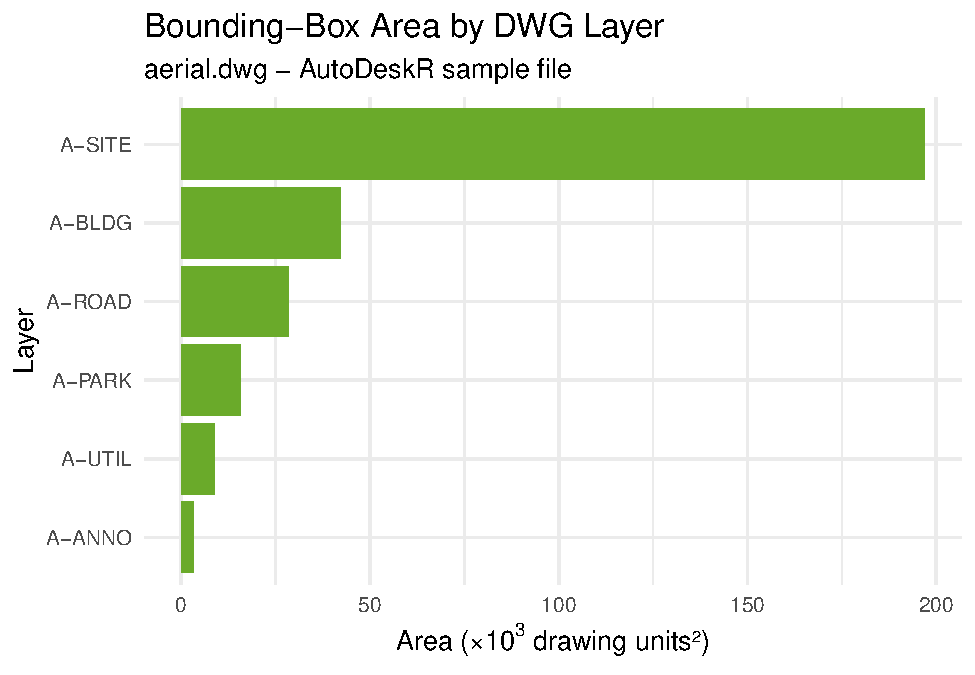
\includegraphics[keepaspectratio]{case-study_files/figure-pdf/unnamed-chunk-7-1.pdf}}

\begin{center}\rule{0.5\linewidth}{0.5pt}\end{center}

\section{Step 6: Build the Shiny
Dashboard}\label{step-6-build-the-shiny-dashboard}

Combine the ggplot2 chart and the embedded 3D viewer in a two-tab Shiny
app:

\begin{Shaded}
\begin{Highlighting}[]
\NormalTok{ui }\OtherTok{\textless{}{-}}\NormalTok{ shiny}\SpecialCharTok{::}\FunctionTok{fluidPage}\NormalTok{(}
\NormalTok{  shiny}\SpecialCharTok{::}\FunctionTok{titlePanel}\NormalTok{(}\StringTok{"Aerial Site — AutoDeskR Case Study"}\NormalTok{),}
\NormalTok{  shiny}\SpecialCharTok{::}\FunctionTok{tabsetPanel}\NormalTok{(}
\NormalTok{    shiny}\SpecialCharTok{::}\FunctionTok{tabPanel}\NormalTok{(}
      \StringTok{"3D Model"}\NormalTok{,}
      \FunctionTok{viewerUI}\NormalTok{(}\StringTok{"model"}\NormalTok{, }\AttributeTok{urn =}\NormalTok{ myEncodedUrn, }\AttributeTok{token =}\NormalTok{ myToken)}
\NormalTok{    ),}
\NormalTok{    shiny}\SpecialCharTok{::}\FunctionTok{tabPanel}\NormalTok{(}
      \StringTok{"Layer Analysis"}\NormalTok{,}
\NormalTok{      shiny}\SpecialCharTok{::}\FunctionTok{plotOutput}\NormalTok{(}\StringTok{"layer\_chart"}\NormalTok{, }\AttributeTok{height =} \StringTok{"500px"}\NormalTok{)}
\NormalTok{    )}
\NormalTok{  )}
\NormalTok{)}

\NormalTok{server }\OtherTok{\textless{}{-}} \ControlFlowTok{function}\NormalTok{(input, output, session) \{}
\NormalTok{  output}\SpecialCharTok{$}\NormalTok{layer\_chart }\OtherTok{\textless{}{-}}\NormalTok{ shiny}\SpecialCharTok{::}\FunctionTok{renderPlot}\NormalTok{(\{}
    \FunctionTok{ggplot}\NormalTok{(layer\_totals, }\FunctionTok{aes}\NormalTok{(}\AttributeTok{x =} \FunctionTok{reorder}\NormalTok{(layer, area), }\AttributeTok{y =}\NormalTok{ area }\SpecialCharTok{/} \DecValTok{1000}\NormalTok{)) }\SpecialCharTok{+}
      \FunctionTok{geom\_col}\NormalTok{(}\AttributeTok{fill =} \StringTok{"\#6aaa2a"}\NormalTok{) }\SpecialCharTok{+}
      \FunctionTok{coord\_flip}\NormalTok{() }\SpecialCharTok{+}
      \FunctionTok{labs}\NormalTok{(}
        \AttributeTok{title =} \StringTok{"Bounding{-}Box Area by DWG Layer"}\NormalTok{,}
        \AttributeTok{x =} \StringTok{"Layer"}\NormalTok{,}
        \AttributeTok{y =} \FunctionTok{expression}\NormalTok{(}\StringTok{"Area (×10"}\SpecialCharTok{\^{}}\DecValTok{3} \SpecialCharTok{*} \StringTok{" units²)"}\NormalTok{)}
\NormalTok{      ) }\SpecialCharTok{+}
      \FunctionTok{theme\_minimal}\NormalTok{(}\AttributeTok{base\_size =} \DecValTok{13}\NormalTok{)}
\NormalTok{  \})}
\NormalTok{\}}

\NormalTok{shiny}\SpecialCharTok{::}\FunctionTok{shinyApp}\NormalTok{(ui, server)}
\end{Highlighting}
\end{Shaded}

The finished dashboard shows the AutoDesk WebGL viewer on the left tab
and the ggplot2 analysis on the right, both driven by data extracted
live from the same DWG file through the APS APIs.

\begin{center}\rule{0.5\linewidth}{0.5pt}\end{center}

\section{Summary}\label{summary}

\begin{longtable}[]{@{}
  >{\raggedright\arraybackslash}p{(\linewidth - 4\tabcolsep) * \real{0.3200}}
  >{\raggedright\arraybackslash}p{(\linewidth - 4\tabcolsep) * \real{0.4400}}
  >{\raggedright\arraybackslash}p{(\linewidth - 4\tabcolsep) * \real{0.2400}}@{}}
\toprule\noalign{}
\begin{minipage}[b]{\linewidth}\raggedright
Step
\end{minipage} & \begin{minipage}[b]{\linewidth}\raggedright
Function(s)
\end{minipage} & \begin{minipage}[b]{\linewidth}\raggedright
API
\end{minipage} \\
\midrule\noalign{}
\endhead
\bottomrule\noalign{}
\endlastfoot
Authenticate & \texttt{getToken()} & Authentication \\
Create bucket + upload & \texttt{makeBucket()}, \texttt{uploadFile()} &
Data Management \\
Translate to SVF & \texttt{translateSvf()}, \texttt{checkFile()} & Model
Derivative \\
Extract properties & \texttt{getMetadata()}, \texttt{getData()} & Model
Derivative \\
Visualise & \texttt{ggplot2} & --- \\
Embed viewer & \texttt{viewerUI()} & Viewer \\
\end{longtable}

The full source for this case study is available at
\href{https://github.com/paulgovan/AutoDeskR}{github.com/paulgovan/AutoDeskR}
in the \texttt{inst/examples/} directory.

\chapter{Function Reference}\label{function-reference}

Quick-lookup table for every exported AutoDeskR function. Click the
\textbf{Chapter} link to jump to full documentation and worked examples.

\section{Authentication}\label{authentication-2}

\begin{longtable}[]{@{}
  >{\raggedright\arraybackslash}p{(\linewidth - 6\tabcolsep) * \real{0.2500}}
  >{\raggedright\arraybackslash}p{(\linewidth - 6\tabcolsep) * \real{0.2500}}
  >{\raggedright\arraybackslash}p{(\linewidth - 6\tabcolsep) * \real{0.2500}}
  >{\raggedright\arraybackslash}p{(\linewidth - 6\tabcolsep) * \real{0.2500}}@{}}
\toprule\noalign{}
\begin{minipage}[b]{\linewidth}\raggedright
Function
\end{minipage} & \begin{minipage}[b]{\linewidth}\raggedright
Required Scopes
\end{minipage} & \begin{minipage}[b]{\linewidth}\raggedright
Key Parameters
\end{minipage} & \begin{minipage}[b]{\linewidth}\raggedright
Returns
\end{minipage} \\
\midrule\noalign{}
\endhead
\bottomrule\noalign{}
\endlastfoot
\texttt{getToken(id,\ secret,\ scope)} & --- & \texttt{id},
\texttt{secret}, \texttt{scope} (space-separated string) &
\texttt{\$content\$access\_token}, \texttt{\$content\$expires\_in} \\
\end{longtable}

\begin{center}\rule{0.5\linewidth}{0.5pt}\end{center}

\section{Data Management}\label{data-management-1}

\begin{longtable}[]{@{}
  >{\raggedright\arraybackslash}p{(\linewidth - 6\tabcolsep) * \real{0.2500}}
  >{\raggedright\arraybackslash}p{(\linewidth - 6\tabcolsep) * \real{0.2500}}
  >{\raggedright\arraybackslash}p{(\linewidth - 6\tabcolsep) * \real{0.2500}}
  >{\raggedright\arraybackslash}p{(\linewidth - 6\tabcolsep) * \real{0.2500}}@{}}
\toprule\noalign{}
\begin{minipage}[b]{\linewidth}\raggedright
Function
\end{minipage} & \begin{minipage}[b]{\linewidth}\raggedright
Required Scopes
\end{minipage} & \begin{minipage}[b]{\linewidth}\raggedright
Key Parameters
\end{minipage} & \begin{minipage}[b]{\linewidth}\raggedright
Returns
\end{minipage} \\
\midrule\noalign{}
\endhead
\bottomrule\noalign{}
\endlastfoot
\texttt{makeBucket(token,\ bucket,\ policy)} & \texttt{bucket:create} &
\texttt{bucket} (globally unique key), \texttt{policy}
(\texttt{"transient"} / \texttt{"temporary"} / \texttt{"persistent"}) &
\texttt{\$content\$bucketKey}, \texttt{\$content\$policyKey} \\
\texttt{checkBucket(token,\ bucket)} & \texttt{bucket:read} &
\texttt{bucket} & \texttt{\$content\$bucketKey},
\texttt{\$content\$policyKey} \\
\texttt{deleteBucket(token,\ bucket)} & \texttt{bucket:delete} &
\texttt{bucket} (must be empty) & \texttt{\$status\_code} 200 \\
\texttt{uploadFile(file,\ token,\ bucket)} & \texttt{data:write} &
\texttt{file} (local path, ≤ 100 MB), \texttt{bucket} &
\texttt{\$content\$objectId} (URN), \texttt{\$content\$size} \\
\texttt{uploadFileSigned(file,\ token,\ bucket)} & \texttt{data:write} &
\texttt{file} (local path, \textgreater{} 100 MB), \texttt{bucket} &
\texttt{\$content\$objectId} (URN) \\
\texttt{listBuckets(token,\ limit,\ startAt,\ region)} &
\texttt{bucket:read} & \texttt{limit} (default 10), \texttt{startAt}
(pagination key), \texttt{region} (\texttt{"US"} / \texttt{"EMEA"}) &
\texttt{\$content\$items} data frame \\
\texttt{listObjects(token,\ bucket,\ limit)} & \texttt{data:read} &
\texttt{bucket}, \texttt{limit} & \texttt{\$content\$items} data
frame \\
\texttt{deleteObject(token,\ bucket,\ object)} & \texttt{data:write} &
\texttt{bucket}, \texttt{object} (filename) & \texttt{\$status\_code}
200 \\
\texttt{downloadFile(urn,\ output\_urn,\ token,\ destfile)} &
\texttt{data:read} & \texttt{urn} (encoded source), \texttt{output\_urn}
(encoded output), \texttt{destfile} & \texttt{\$status\_code} 200 \\
\end{longtable}

\begin{center}\rule{0.5\linewidth}{0.5pt}\end{center}

\section{Model Derivative}\label{model-derivative-1}

\begin{longtable}[]{@{}
  >{\raggedright\arraybackslash}p{(\linewidth - 6\tabcolsep) * \real{0.2500}}
  >{\raggedright\arraybackslash}p{(\linewidth - 6\tabcolsep) * \real{0.2500}}
  >{\raggedright\arraybackslash}p{(\linewidth - 6\tabcolsep) * \real{0.2500}}
  >{\raggedright\arraybackslash}p{(\linewidth - 6\tabcolsep) * \real{0.2500}}@{}}
\toprule\noalign{}
\begin{minipage}[b]{\linewidth}\raggedright
Function
\end{minipage} & \begin{minipage}[b]{\linewidth}\raggedright
Required Scopes
\end{minipage} & \begin{minipage}[b]{\linewidth}\raggedright
Key Parameters
\end{minipage} & \begin{minipage}[b]{\linewidth}\raggedright
Returns
\end{minipage} \\
\midrule\noalign{}
\endhead
\bottomrule\noalign{}
\endlastfoot
\texttt{translateObj(urn,\ token)} & \texttt{data:read\ data:write} &
\texttt{urn} (Base-64 encoded) & \texttt{\$content\$result}
(\texttt{"created"}), \texttt{\$content\$urn} \\
\texttt{translateStl(urn,\ token)} & \texttt{data:read\ data:write} &
\texttt{urn} (Base-64 encoded) & \texttt{\$content\$result},
\texttt{\$content\$urn} \\
\texttt{translateSvf(urn,\ token)} & \texttt{data:read\ data:write} &
\texttt{urn} (Base-64 encoded) & \texttt{\$content\$result},
\texttt{\$content\$urn} \\
\texttt{checkFile(urn,\ token)} & \texttt{data:read} & \texttt{urn}
(Base-64 encoded) & \texttt{\$content\$status} (\texttt{"pending"} /
\texttt{"inprogress"} / \texttt{"success"}),
\texttt{\$content\$progress} \\
\texttt{getOutputUrn(urn,\ token)} & \texttt{data:read} & \texttt{urn}
(raw, not encoded) &
\texttt{\$content\$derivatives{[}{[}1{]}{]}\$children{[}{[}1{]}{]}\$urn} \\
\texttt{getMetadata(urn,\ token)} & \texttt{data:read} & \texttt{urn}
(Base-64 encoded) &
\texttt{\$content\$data\$metadata{[}{[}1{]}{]}\$guid},
\texttt{\$content\$data\$metadata{[}{[}1{]}{]}\$name} \\
\texttt{getObjectTree(guid,\ urn,\ token)} & \texttt{data:read} &
\texttt{guid}, \texttt{urn} (Base-64 encoded) &
\texttt{\$content\$data\$objects} (nested list) \\
\texttt{getData(guid,\ urn,\ token)} & \texttt{data:read} &
\texttt{guid}, \texttt{urn} (Base-64 encoded) &
\texttt{\$content\$data\$collection} (list of objects with
properties) \\
\end{longtable}

\begin{center}\rule{0.5\linewidth}{0.5pt}\end{center}

\section{Design Automation}\label{design-automation-1}

\begin{longtable}[]{@{}
  >{\raggedright\arraybackslash}p{(\linewidth - 6\tabcolsep) * \real{0.2500}}
  >{\raggedright\arraybackslash}p{(\linewidth - 6\tabcolsep) * \real{0.2500}}
  >{\raggedright\arraybackslash}p{(\linewidth - 6\tabcolsep) * \real{0.2500}}
  >{\raggedright\arraybackslash}p{(\linewidth - 6\tabcolsep) * \real{0.2500}}@{}}
\toprule\noalign{}
\begin{minipage}[b]{\linewidth}\raggedright
Function
\end{minipage} & \begin{minipage}[b]{\linewidth}\raggedright
Required Scopes
\end{minipage} & \begin{minipage}[b]{\linewidth}\raggedright
Key Parameters
\end{minipage} & \begin{minipage}[b]{\linewidth}\raggedright
Returns
\end{minipage} \\
\midrule\noalign{}
\endhead
\bottomrule\noalign{}
\endlastfoot
\texttt{makePdf(source,\ destination,\ token)} & \texttt{code:all} &
\texttt{source} (public URL to DWG), \texttt{destination} (public URL
for output) & \texttt{\$content\$id} (WorkItem ID),
\texttt{\$content\$status} \\
\texttt{checkPdf(id,\ token)} & \texttt{code:all} & \texttt{id}
(WorkItem ID from \texttt{makePdf()}) & \texttt{\$content\$status}
(\texttt{"pending"} / \texttt{"inprogress"} / \texttt{"success"}),
\texttt{\$content\$stats} \\
\end{longtable}

\begin{center}\rule{0.5\linewidth}{0.5pt}\end{center}

\section{Reality Capture}\label{reality-capture-1}

\begin{longtable}[]{@{}
  >{\raggedright\arraybackslash}p{(\linewidth - 6\tabcolsep) * \real{0.2500}}
  >{\raggedright\arraybackslash}p{(\linewidth - 6\tabcolsep) * \real{0.2500}}
  >{\raggedright\arraybackslash}p{(\linewidth - 6\tabcolsep) * \real{0.2500}}
  >{\raggedright\arraybackslash}p{(\linewidth - 6\tabcolsep) * \real{0.2500}}@{}}
\toprule\noalign{}
\begin{minipage}[b]{\linewidth}\raggedright
Function
\end{minipage} & \begin{minipage}[b]{\linewidth}\raggedright
Required Scopes
\end{minipage} & \begin{minipage}[b]{\linewidth}\raggedright
Key Parameters
\end{minipage} & \begin{minipage}[b]{\linewidth}\raggedright
Returns
\end{minipage} \\
\midrule\noalign{}
\endhead
\bottomrule\noalign{}
\endlastfoot
\texttt{createPhotoscene(name,\ format,\ token)} &
\texttt{data:read\ data:write} & \texttt{name} (scene label),
\texttt{format} (\texttt{"rcm"} / \texttt{"rcs"} / \texttt{"obj"} /
\texttt{"ortho"} / \texttt{"report"}) &
\texttt{\$content\$photoscene\$photosceneid} \\
\texttt{uploadImages(photoscene\_id,\ files,\ token)} &
\texttt{data:read\ data:write} & \texttt{photoscene\_id}, \texttt{files}
(character vector of local JPEG/PNG paths) &
\texttt{\$content\$Files\$file} (list of uploaded file records) \\
\texttt{processPhotoscene(photoscene\_id,\ token)} &
\texttt{data:read\ data:write} & \texttt{photoscene\_id} &
\texttt{\$content\$photoscene\$progress} (\texttt{"0"} on submission) \\
\texttt{checkPhotoscene(photoscene\_id,\ token)} &
\texttt{data:read\ data:write} & \texttt{photoscene\_id} &
\texttt{\$content\$photoscene\$progress} (string
\texttt{"0"}--\texttt{"100"}),
\texttt{\$content\$photoscene\$progressmsg} \\
\texttt{waitForPhotoscene(photoscene\_id,\ token,\ interval,\ timeout,\ verbose)}
& \texttt{data:read\ data:write} & \texttt{interval} (seconds between
polls, default 30), \texttt{timeout} (max wait in seconds, default 1800)
& Final \texttt{checkPhotoscene} response when
\texttt{progress\ ==\ "100"} \\
\end{longtable}

\begin{center}\rule{0.5\linewidth}{0.5pt}\end{center}

\section{Viewer}\label{viewer-1}

\begin{longtable}[]{@{}
  >{\raggedright\arraybackslash}p{(\linewidth - 6\tabcolsep) * \real{0.2500}}
  >{\raggedright\arraybackslash}p{(\linewidth - 6\tabcolsep) * \real{0.2500}}
  >{\raggedright\arraybackslash}p{(\linewidth - 6\tabcolsep) * \real{0.2500}}
  >{\raggedright\arraybackslash}p{(\linewidth - 6\tabcolsep) * \real{0.2500}}@{}}
\toprule\noalign{}
\begin{minipage}[b]{\linewidth}\raggedright
Function
\end{minipage} & \begin{minipage}[b]{\linewidth}\raggedright
Required Scopes
\end{minipage} & \begin{minipage}[b]{\linewidth}\raggedright
Key Parameters
\end{minipage} & \begin{minipage}[b]{\linewidth}\raggedright
Returns
\end{minipage} \\
\midrule\noalign{}
\endhead
\bottomrule\noalign{}
\endlastfoot
\texttt{viewer3D(urn,\ token,\ viewerType)} & \texttt{data:read} &
\texttt{urn} (Base-64 encoded), \texttt{viewerType} (\texttt{"header"} /
\texttt{"headless"} / \texttt{"vr"}) & Opens viewer in browser /
Shiny \\
\texttt{viewerUI(id,\ urn,\ token,\ viewerType)} & \texttt{data:read} &
\texttt{id} (Shiny module ID), \texttt{urn}, \texttt{token},
\texttt{viewerType} & Shiny UI element for use in
\texttt{fluidPage()} \\
\end{longtable}

\begin{center}\rule{0.5\linewidth}{0.5pt}\end{center}

\section{Scope Quick Reference}\label{scope-quick-reference}

\begin{longtable}[]{@{}
  >{\raggedright\arraybackslash}p{(\linewidth - 2\tabcolsep) * \real{0.5000}}
  >{\raggedright\arraybackslash}p{(\linewidth - 2\tabcolsep) * \real{0.5000}}@{}}
\toprule\noalign{}
\begin{minipage}[b]{\linewidth}\raggedright
Scope
\end{minipage} & \begin{minipage}[b]{\linewidth}\raggedright
Used by
\end{minipage} \\
\midrule\noalign{}
\endhead
\bottomrule\noalign{}
\endlastfoot
\texttt{data:read} & Model Derivative, Viewer, Reality Capture (read) \\
\texttt{data:write} & Data Management (upload/delete), Model Derivative
(translate), Reality Capture \\
\texttt{bucket:create} & Data Management (\texttt{makeBucket}) \\
\texttt{bucket:read} & Data Management (\texttt{checkBucket},
\texttt{listBuckets}) \\
\texttt{bucket:delete} & Data Management (\texttt{deleteBucket}) \\
\texttt{code:all} & Design Automation \\
\end{longtable}

\section{Common Patterns}\label{common-patterns}

\subsection{Base-64 encode a URN}\label{base-64-encode-a-urn}

The Model Derivative and Viewer APIs require the URN to be Base-64
encoded. Use \texttt{jsonlite::base64\_enc()}:

\begin{Shaded}
\begin{Highlighting}[]
\NormalTok{myEncodedUrn }\OtherTok{\textless{}{-}}\NormalTok{ jsonlite}\SpecialCharTok{::}\FunctionTok{base64\_enc}\NormalTok{(myUrn)}
\end{Highlighting}
\end{Shaded}

\subsection{Poll until a job finishes}\label{poll-until-a-job-finishes}

All async jobs (\texttt{translateObj}, \texttt{translateSvf},
\texttt{makePdf}, \texttt{processPhotoscene}) follow the same pattern:

\begin{Shaded}
\begin{Highlighting}[]
\ControlFlowTok{repeat}\NormalTok{ \{}
\NormalTok{  status }\OtherTok{\textless{}{-}} \FunctionTok{checkFile}\NormalTok{(}\AttributeTok{urn =}\NormalTok{ myEncodedUrn, }\AttributeTok{token =}\NormalTok{ myToken)}
  \ControlFlowTok{if}\NormalTok{ (status}\SpecialCharTok{$}\NormalTok{content}\SpecialCharTok{$}\NormalTok{status }\SpecialCharTok{==} \StringTok{"success"}\NormalTok{) }\ControlFlowTok{break}
  \FunctionTok{Sys.sleep}\NormalTok{(}\DecValTok{10}\NormalTok{)}
\NormalTok{\}}
\end{Highlighting}
\end{Shaded}

Use \texttt{waitForPhotoscene()} as a ready-made equivalent for Reality
Capture jobs.

\begin{center}\rule{0.5\linewidth}{0.5pt}\end{center}

\chapter{Supporting Packages}\label{supporting-packages}

The chapters outside the Core APIs part rely on the following R
packages. This section lists the key functions used in the book and the
chapter where each appears.

\begin{center}\rule{0.5\linewidth}{0.5pt}\end{center}

\section{httr2}\label{httr2}

Used for direct Tandem REST API calls in the Digital Twins chapters, and
as the underlying HTTP engine for AutoDeskR.

\begin{longtable}[]{@{}
  >{\raggedright\arraybackslash}p{(\linewidth - 4\tabcolsep) * \real{0.3333}}
  >{\raggedright\arraybackslash}p{(\linewidth - 4\tabcolsep) * \real{0.3333}}
  >{\raggedright\arraybackslash}p{(\linewidth - 4\tabcolsep) * \real{0.3333}}@{}}
\toprule\noalign{}
\begin{minipage}[b]{\linewidth}\raggedright
Function
\end{minipage} & \begin{minipage}[b]{\linewidth}\raggedright
Description
\end{minipage} & \begin{minipage}[b]{\linewidth}\raggedright
Chapter
\end{minipage} \\
\midrule\noalign{}
\endhead
\bottomrule\noalign{}
\endlastfoot
\texttt{request(url)} & Create a new HTTP request &
\hyperref[autodesk-tandem-overview]{Tandem Overview},
\hyperref[linking-sensor-streams]{Sensor Streams} \\
\texttt{req\_auth\_bearer\_token(req,\ token)} & Add a Bearer token
header & \hyperref[autodesk-tandem-overview]{Tandem Overview} \\
\texttt{req\_url\_query(req,\ ...)} & Append query parameters &
\hyperref[linking-sensor-streams]{Sensor Streams} \\
\texttt{req\_perform(req)} & Execute the request &
\hyperref[autodesk-tandem-overview]{Tandem Overview} \\
\texttt{req\_verbose()} & Enable request/response tracing &
\href{troubleshooting.qmd}{Troubleshooting} \\
\texttt{resp\_body\_json(resp)} & Parse response body as JSON &
\hyperref[linking-sensor-streams]{Sensor Streams} \\
\end{longtable}

\begin{center}\rule{0.5\linewidth}{0.5pt}\end{center}

\section{jsonlite}\label{jsonlite}

\begin{longtable}[]{@{}
  >{\raggedright\arraybackslash}p{(\linewidth - 4\tabcolsep) * \real{0.3333}}
  >{\raggedright\arraybackslash}p{(\linewidth - 4\tabcolsep) * \real{0.3333}}
  >{\raggedright\arraybackslash}p{(\linewidth - 4\tabcolsep) * \real{0.3333}}@{}}
\toprule\noalign{}
\begin{minipage}[b]{\linewidth}\raggedright
Function
\end{minipage} & \begin{minipage}[b]{\linewidth}\raggedright
Description
\end{minipage} & \begin{minipage}[b]{\linewidth}\raggedright
Chapter
\end{minipage} \\
\midrule\noalign{}
\endhead
\bottomrule\noalign{}
\endlastfoot
\texttt{base64\_enc(x)} & Base-64 encode a string (required for APS
URNs) & \hyperref[model-derivative]{Model Derivative},
\hyperref[case-study-dwg-to-shiny-dashboard]{Case Study} \\
\texttt{fromJSON(txt)} & Parse a JSON string into an R list & General \\
\end{longtable}

\begin{center}\rule{0.5\linewidth}{0.5pt}\end{center}

\section{Rvcg}\label{rvcg}

Mesh processing --- surface area, volume, smoothing, and surface
distance. (Schlager 2024)

\begin{longtable}[]{@{}
  >{\raggedright\arraybackslash}p{(\linewidth - 4\tabcolsep) * \real{0.3333}}
  >{\raggedright\arraybackslash}p{(\linewidth - 4\tabcolsep) * \real{0.3333}}
  >{\raggedright\arraybackslash}p{(\linewidth - 4\tabcolsep) * \real{0.3333}}@{}}
\toprule\noalign{}
\begin{minipage}[b]{\linewidth}\raggedright
Function
\end{minipage} & \begin{minipage}[b]{\linewidth}\raggedright
Description
\end{minipage} & \begin{minipage}[b]{\linewidth}\raggedright
Chapter
\end{minipage} \\
\midrule\noalign{}
\endhead
\bottomrule\noalign{}
\endlastfoot
\texttt{vcgImport(file)} & Import OBJ, STL, or PLY mesh as
\texttt{tmesh3d} & \hyperref[reading-obj-and-stl-meshes]{Reading
Meshes} \\
\texttt{vcgArea(mesh)} & Compute total surface area &
\hyperref[mesh-metrics]{Mesh Metrics} \\
\texttt{vcgVolume(mesh)} & Compute volume (watertight meshes only) &
\hyperref[mesh-metrics]{Mesh Metrics} \\
\texttt{vcgSmooth(mesh,\ iteration,\ lambda)} & Laplacian smoothing &
\hyperref[mesh-comparison]{Mesh Comparison} \\
\texttt{vcgDist(mesh1,\ mesh2)} & Per-vertex surface distance &
\hyperref[mesh-comparison]{Mesh Comparison} \\
\end{longtable}

\begin{center}\rule{0.5\linewidth}{0.5pt}\end{center}

\section{rgl}\label{rgl}

Interactive 3D visualisation. (Adler, Murdoch, et al. 2024)

\begin{longtable}[]{@{}
  >{\raggedright\arraybackslash}p{(\linewidth - 4\tabcolsep) * \real{0.3333}}
  >{\raggedright\arraybackslash}p{(\linewidth - 4\tabcolsep) * \real{0.3333}}
  >{\raggedright\arraybackslash}p{(\linewidth - 4\tabcolsep) * \real{0.3333}}@{}}
\toprule\noalign{}
\begin{minipage}[b]{\linewidth}\raggedright
Function
\end{minipage} & \begin{minipage}[b]{\linewidth}\raggedright
Description
\end{minipage} & \begin{minipage}[b]{\linewidth}\raggedright
Chapter
\end{minipage} \\
\midrule\noalign{}
\endhead
\bottomrule\noalign{}
\endlastfoot
\texttt{open3d()} & Open a new 3D graphics device &
\hyperref[d-visualisation]{Mesh Visualisation} \\
\texttt{shade3d(mesh,\ col)} & Render a mesh with per-vertex colours &
\hyperref[d-visualisation]{Mesh Visualisation},
\hyperref[mesh-comparison]{Mesh Comparison} \\
\texttt{rglwidget()} & Embed interactive 3D widget in HTML &
\hyperref[d-visualisation]{Mesh Visualisation} \\
\texttt{readOBJ(file)} & Alternative OBJ reader &
\href{troubleshooting.qmd}{Troubleshooting} \\
\texttt{options(rgl.useNULL\ =\ TRUE)} & Suppress OpenGL window
(headless/server use) & \href{troubleshooting.qmd}{Troubleshooting} \\
\end{longtable}

\begin{center}\rule{0.5\linewidth}{0.5pt}\end{center}

\section{geometry}\label{geometry}

Computational geometry for open (non-watertight) meshes. (Roussel,
Sterratt, et al. 2024)

\begin{longtable}[]{@{}
  >{\raggedright\arraybackslash}p{(\linewidth - 4\tabcolsep) * \real{0.3333}}
  >{\raggedright\arraybackslash}p{(\linewidth - 4\tabcolsep) * \real{0.3333}}
  >{\raggedright\arraybackslash}p{(\linewidth - 4\tabcolsep) * \real{0.3333}}@{}}
\toprule\noalign{}
\begin{minipage}[b]{\linewidth}\raggedright
Function
\end{minipage} & \begin{minipage}[b]{\linewidth}\raggedright
Description
\end{minipage} & \begin{minipage}[b]{\linewidth}\raggedright
Chapter
\end{minipage} \\
\midrule\noalign{}
\endhead
\bottomrule\noalign{}
\endlastfoot
\texttt{convhulln(pts,\ options)} & Convex hull with area and volume
(\texttt{options\ =\ "FA"}) & \hyperref[mesh-metrics]{Mesh Metrics} \\
\end{longtable}

\begin{center}\rule{0.5\linewidth}{0.5pt}\end{center}

\section{rayshader}\label{rayshader}

High-quality 3D rendered images. (Morgan-Wall 2024)

\begin{longtable}[]{@{}
  >{\raggedright\arraybackslash}p{(\linewidth - 4\tabcolsep) * \real{0.3333}}
  >{\raggedright\arraybackslash}p{(\linewidth - 4\tabcolsep) * \real{0.3333}}
  >{\raggedright\arraybackslash}p{(\linewidth - 4\tabcolsep) * \real{0.3333}}@{}}
\toprule\noalign{}
\begin{minipage}[b]{\linewidth}\raggedright
Function
\end{minipage} & \begin{minipage}[b]{\linewidth}\raggedright
Description
\end{minipage} & \begin{minipage}[b]{\linewidth}\raggedright
Chapter
\end{minipage} \\
\midrule\noalign{}
\endhead
\bottomrule\noalign{}
\endlastfoot
\texttt{render\_snapshot(filename)} & Save a ray-traced render to file &
\hyperref[d-visualisation]{Mesh Visualisation} \\
\end{longtable}

\begin{center}\rule{0.5\linewidth}{0.5pt}\end{center}

\section{lidR}\label{lidr}

Point cloud analysis from LAS/LAZ files. (Roussel et al. 2020)

\begin{longtable}[]{@{}
  >{\raggedright\arraybackslash}p{(\linewidth - 4\tabcolsep) * \real{0.3333}}
  >{\raggedright\arraybackslash}p{(\linewidth - 4\tabcolsep) * \real{0.3333}}
  >{\raggedright\arraybackslash}p{(\linewidth - 4\tabcolsep) * \real{0.3333}}@{}}
\toprule\noalign{}
\begin{minipage}[b]{\linewidth}\raggedright
Function
\end{minipage} & \begin{minipage}[b]{\linewidth}\raggedright
Description
\end{minipage} & \begin{minipage}[b]{\linewidth}\raggedright
Chapter
\end{minipage} \\
\midrule\noalign{}
\endhead
\bottomrule\noalign{}
\endlastfoot
\texttt{readLAS(file)} & Read a LAS or LAZ point cloud &
\hyperref[point-cloud-analysis]{Point Cloud Analysis} \\
\texttt{normalize\_height(pc,\ algorithm)} & Normalise Z to ground level
& \hyperref[point-cloud-analysis]{Point Cloud Analysis} \\
\texttt{rasterize\_canopy(pc,\ res,\ algorithm)} & Maximum-Z raster
(canopy/roof height model) & \hyperref[point-cloud-analysis]{Point Cloud
Analysis} \\
\texttt{grid\_density(pc,\ res)} & Point density raster &
\hyperref[point-cloud-analysis]{Point Cloud Analysis} \\
\texttt{voxelize\_points(pc,\ res)} & Voxelise point cloud for volume
estimation & \hyperref[point-cloud-analysis]{Point Cloud Analysis} \\
\texttt{npoints(pc)} & Total point count &
\hyperref[point-cloud-analysis]{Point Cloud Analysis} \\
\texttt{area(pc)} & Survey footprint area &
\hyperref[point-cloud-analysis]{Point Cloud Analysis} \\
\end{longtable}

\begin{center}\rule{0.5\linewidth}{0.5pt}\end{center}

\section{dplyr}\label{dplyr}

Data manipulation --- filtering, grouping, joining. Used throughout the
DWG Analytics and Digital Twins chapters.

\begin{longtable}[]{@{}
  >{\raggedright\arraybackslash}p{(\linewidth - 4\tabcolsep) * \real{0.3333}}
  >{\raggedright\arraybackslash}p{(\linewidth - 4\tabcolsep) * \real{0.3333}}
  >{\raggedright\arraybackslash}p{(\linewidth - 4\tabcolsep) * \real{0.3333}}@{}}
\toprule\noalign{}
\begin{minipage}[b]{\linewidth}\raggedright
Function
\end{minipage} & \begin{minipage}[b]{\linewidth}\raggedright
Description
\end{minipage} & \begin{minipage}[b]{\linewidth}\raggedright
Chapter
\end{minipage} \\
\midrule\noalign{}
\endhead
\bottomrule\noalign{}
\endlastfoot
\texttt{group\_by(...)} & Group rows for summarisation &
\hyperref[layer-structure-analysis]{Layer Analysis} \\
\texttt{summarise(...)} & Aggregate within groups &
\hyperref[layer-structure-analysis]{Layer Analysis} \\
\texttt{filter(...)} & Keep rows matching a condition &
\hyperref[attribute-extraction]{Attribute Extraction} \\
\texttt{select(...)} & Choose columns &
\hyperref[linking-sensor-streams]{Sensor Streams} \\
\texttt{mutate(...)} & Add or transform columns &
\hyperref[attribute-extraction]{Attribute Extraction} \\
\texttt{inner\_join(x,\ y,\ by)} & Join keeping rows in both tables &
\hyperref[linking-sensor-streams]{Sensor Streams} \\
\texttt{left\_join(x,\ y,\ by)} & Join keeping all rows from left table
& \hyperref[linking-sensor-streams]{Sensor Streams} \\
\end{longtable}

\begin{center}\rule{0.5\linewidth}{0.5pt}\end{center}

\section{tidyr}\label{tidyr}

\begin{longtable}[]{@{}
  >{\raggedright\arraybackslash}p{(\linewidth - 4\tabcolsep) * \real{0.3333}}
  >{\raggedright\arraybackslash}p{(\linewidth - 4\tabcolsep) * \real{0.3333}}
  >{\raggedright\arraybackslash}p{(\linewidth - 4\tabcolsep) * \real{0.3333}}@{}}
\toprule\noalign{}
\begin{minipage}[b]{\linewidth}\raggedright
Function
\end{minipage} & \begin{minipage}[b]{\linewidth}\raggedright
Description
\end{minipage} & \begin{minipage}[b]{\linewidth}\raggedright
Chapter
\end{minipage} \\
\midrule\noalign{}
\endhead
\bottomrule\noalign{}
\endlastfoot
\texttt{pivot\_wider(data,\ names\_from,\ values\_from)} & Reshape long
data to wide format & \hyperref[attribute-extraction]{Attribute
Extraction} \\
\end{longtable}

\begin{center}\rule{0.5\linewidth}{0.5pt}\end{center}

\section{ggplot2}\label{ggplot2}

Data visualisation. Used in DWG Analytics, Digital Twins, and the Case
Study.

\begin{longtable}[]{@{}
  >{\raggedright\arraybackslash}p{(\linewidth - 4\tabcolsep) * \real{0.3333}}
  >{\raggedright\arraybackslash}p{(\linewidth - 4\tabcolsep) * \real{0.3333}}
  >{\raggedright\arraybackslash}p{(\linewidth - 4\tabcolsep) * \real{0.3333}}@{}}
\toprule\noalign{}
\begin{minipage}[b]{\linewidth}\raggedright
Function
\end{minipage} & \begin{minipage}[b]{\linewidth}\raggedright
Description
\end{minipage} & \begin{minipage}[b]{\linewidth}\raggedright
Chapter
\end{minipage} \\
\midrule\noalign{}
\endhead
\bottomrule\noalign{}
\endlastfoot
\texttt{ggplot(data,\ aes(...))} & Initialise a plot & Multiple \\
\texttt{geom\_col()} & Bar chart (pre-counted values) &
\hyperref[layer-structure-analysis]{Layer Analysis} \\
\texttt{geom\_line()} & Line chart &
\hyperref[linking-sensor-streams]{Sensor Streams} \\
\texttt{geom\_histogram()} & Histogram &
\hyperref[point-cloud-analysis]{Point Cloud Analysis},
\hyperref[mesh-comparison]{Mesh Comparison} \\
\texttt{geom\_ribbon()} & Shaded confidence band &
\hyperref[linking-sensor-streams]{Sensor Streams} \\
\texttt{geom\_tile()} & Heatmap tiles &
\hyperref[cross-drawing-comparison]{Cross-Drawing Comparison} \\
\texttt{facet\_wrap(\textasciitilde{}\ var)} & Small multiples &
\hyperref[linking-sensor-streams]{Sensor Streams} \\
\texttt{coord\_flip()} & Swap x and y axes &
\hyperref[layer-structure-analysis]{Layer Analysis} \\
\texttt{theme\_minimal()} & Clean theme & Multiple \\
\end{longtable}

\begin{center}\rule{0.5\linewidth}{0.5pt}\end{center}

\section{gt}\label{gt}

Publication-quality tables for automated reports.(Iannone et al. 2024)

\begin{longtable}[]{@{}
  >{\raggedright\arraybackslash}p{(\linewidth - 4\tabcolsep) * \real{0.3333}}
  >{\raggedright\arraybackslash}p{(\linewidth - 4\tabcolsep) * \real{0.3333}}
  >{\raggedright\arraybackslash}p{(\linewidth - 4\tabcolsep) * \real{0.3333}}@{}}
\toprule\noalign{}
\begin{minipage}[b]{\linewidth}\raggedright
Function
\end{minipage} & \begin{minipage}[b]{\linewidth}\raggedright
Description
\end{minipage} & \begin{minipage}[b]{\linewidth}\raggedright
Chapter
\end{minipage} \\
\midrule\noalign{}
\endhead
\bottomrule\noalign{}
\endlastfoot
\texttt{gt(data)} & Create a gt table from a data frame &
\hyperref[automated-drawing-reports]{Drawing Reports} \\
\texttt{tab\_header(title,\ subtitle)} & Add a title and subtitle &
\hyperref[automated-drawing-reports]{Drawing Reports} \\
\texttt{fmt\_number(columns,\ decimals)} & Format numeric columns &
\hyperref[automated-drawing-reports]{Drawing Reports} \\
\texttt{cols\_label(...)} & Rename column headers &
\hyperref[automated-drawing-reports]{Drawing Reports} \\
\texttt{tab\_source\_note(note)} & Add a footnote &
\hyperref[automated-drawing-reports]{Drawing Reports} \\
\end{longtable}

\begin{center}\rule{0.5\linewidth}{0.5pt}\end{center}

\section{shiny}\label{shiny}

Interactive web applications and dashboards.

\begin{longtable}[]{@{}
  >{\raggedright\arraybackslash}p{(\linewidth - 4\tabcolsep) * \real{0.3333}}
  >{\raggedright\arraybackslash}p{(\linewidth - 4\tabcolsep) * \real{0.3333}}
  >{\raggedright\arraybackslash}p{(\linewidth - 4\tabcolsep) * \real{0.3333}}@{}}
\toprule\noalign{}
\begin{minipage}[b]{\linewidth}\raggedright
Function
\end{minipage} & \begin{minipage}[b]{\linewidth}\raggedright
Description
\end{minipage} & \begin{minipage}[b]{\linewidth}\raggedright
Chapter
\end{minipage} \\
\midrule\noalign{}
\endhead
\bottomrule\noalign{}
\endlastfoot
\texttt{fluidPage(...)} & Standard responsive page layout &
\hyperref[viewer]{Viewer}, \hyperref[live-dashboards]{Live
Dashboards} \\
\texttt{tabsetPanel(...)} / \texttt{tabPanel(...)} & Tabbed layout &
\hyperref[case-study-dwg-to-shiny-dashboard]{Case Study} \\
\texttt{renderPlot(\{\})} & Reactive ggplot2 output &
\hyperref[case-study-dwg-to-shiny-dashboard]{Case Study} \\
\texttt{plotOutput(id)} & Placeholder for a plot &
\hyperref[case-study-dwg-to-shiny-dashboard]{Case Study} \\
\texttt{reactiveTimer(ms)} & Trigger reactive updates on a schedule &
\hyperref[live-dashboards]{Live Dashboards} \\
\texttt{shinyApp(ui,\ server)} & Launch the app &
\hyperref[case-study-dwg-to-shiny-dashboard]{Case Study} \\
\texttt{deployApp()} & Deploy to shinyapps.io &
\hyperref[live-dashboards]{Live Dashboards} \\
\end{longtable}

\begin{center}\rule{0.5\linewidth}{0.5pt}\end{center}

\section{dygraphs}\label{dygraphs}

Interactive time-series plots for Shiny dashboards. (Vanderkam et al.
2018)

\begin{longtable}[]{@{}
  >{\raggedright\arraybackslash}p{(\linewidth - 4\tabcolsep) * \real{0.3333}}
  >{\raggedright\arraybackslash}p{(\linewidth - 4\tabcolsep) * \real{0.3333}}
  >{\raggedright\arraybackslash}p{(\linewidth - 4\tabcolsep) * \real{0.3333}}@{}}
\toprule\noalign{}
\begin{minipage}[b]{\linewidth}\raggedright
Function
\end{minipage} & \begin{minipage}[b]{\linewidth}\raggedright
Description
\end{minipage} & \begin{minipage}[b]{\linewidth}\raggedright
Chapter
\end{minipage} \\
\midrule\noalign{}
\endhead
\bottomrule\noalign{}
\endlastfoot
\texttt{dygraph(data,\ main)} & Create an interactive time-series chart
& \hyperref[live-dashboards]{Live Dashboards} \\
\texttt{dyOptions(...)} & Customise colours, fill, axes &
\hyperref[live-dashboards]{Live Dashboards} \\
\texttt{dygraphOutput(id)} & Shiny UI placeholder &
\hyperref[live-dashboards]{Live Dashboards} \\
\texttt{renderDygraph(\{\})} & Shiny server renderer &
\hyperref[live-dashboards]{Live Dashboards} \\
\end{longtable}

\begin{center}\rule{0.5\linewidth}{0.5pt}\end{center}

\section{xts}\label{xts}

Time-series objects required by \texttt{dygraphs}.

\begin{longtable}[]{@{}
  >{\raggedright\arraybackslash}p{(\linewidth - 4\tabcolsep) * \real{0.3333}}
  >{\raggedright\arraybackslash}p{(\linewidth - 4\tabcolsep) * \real{0.3333}}
  >{\raggedright\arraybackslash}p{(\linewidth - 4\tabcolsep) * \real{0.3333}}@{}}
\toprule\noalign{}
\begin{minipage}[b]{\linewidth}\raggedright
Function
\end{minipage} & \begin{minipage}[b]{\linewidth}\raggedright
Description
\end{minipage} & \begin{minipage}[b]{\linewidth}\raggedright
Chapter
\end{minipage} \\
\midrule\noalign{}
\endhead
\bottomrule\noalign{}
\endlastfoot
\texttt{xts(data,\ order.by)} & Create an extensible time-series object
& \hyperref[live-dashboards]{Live Dashboards} \\
\end{longtable}

\begin{center}\rule{0.5\linewidth}{0.5pt}\end{center}

\section{quarto}\label{quarto}

Programmatic report rendering.

\begin{longtable}[]{@{}
  >{\raggedright\arraybackslash}p{(\linewidth - 4\tabcolsep) * \real{0.3333}}
  >{\raggedright\arraybackslash}p{(\linewidth - 4\tabcolsep) * \real{0.3333}}
  >{\raggedright\arraybackslash}p{(\linewidth - 4\tabcolsep) * \real{0.3333}}@{}}
\toprule\noalign{}
\begin{minipage}[b]{\linewidth}\raggedright
Function
\end{minipage} & \begin{minipage}[b]{\linewidth}\raggedright
Description
\end{minipage} & \begin{minipage}[b]{\linewidth}\raggedright
Chapter
\end{minipage} \\
\midrule\noalign{}
\endhead
\bottomrule\noalign{}
\endlastfoot
\texttt{quarto\_render(input,\ execute\_params)} & Render a
\texttt{.qmd} file with injected parameters &
\hyperref[automated-drawing-reports]{Drawing Reports} \\
\end{longtable}

\chapter{Troubleshooting}\label{troubleshooting}

Something's not working. Don't worry. APS errors are usually pretty
informative once you know how to read them. This chapter is a reference
for the most common problems, organised by HTTP status code and then by
API area.

\section{Error Code Quick Reference}\label{error-code-quick-reference}

The first thing to check is always \texttt{resp\$status\_code}. Here's
what each code means and where to start looking:

\begin{longtable}[]{@{}
  >{\raggedright\arraybackslash}p{(\linewidth - 6\tabcolsep) * \real{0.2500}}
  >{\raggedright\arraybackslash}p{(\linewidth - 6\tabcolsep) * \real{0.2500}}
  >{\raggedright\arraybackslash}p{(\linewidth - 6\tabcolsep) * \real{0.2500}}
  >{\raggedright\arraybackslash}p{(\linewidth - 6\tabcolsep) * \real{0.2500}}@{}}
\toprule\noalign{}
\begin{minipage}[b]{\linewidth}\raggedright
Code
\end{minipage} & \begin{minipage}[b]{\linewidth}\raggedright
Meaning
\end{minipage} & \begin{minipage}[b]{\linewidth}\raggedright
Most likely cause
\end{minipage} & \begin{minipage}[b]{\linewidth}\raggedright
First step
\end{minipage} \\
\midrule\noalign{}
\endhead
\bottomrule\noalign{}
\endlastfoot
400 & Bad Request & Malformed request body; non-public URL in Design
Automation & Check source/destination URLs; validate parameters \\
401 & Unauthorized & Token expired or missing; wrong scope & Re-call
\texttt{getToken()} with correct scopes \\
403 & Forbidden & Free-tier quota exceeded; API not enabled for app &
Check quota in APS portal; enable the API on your app \\
404 & Not Found & Wrong URN; object or bucket deleted; bad GUID &
Re-check URN encoding; confirm the resource exists \\
409 & Conflict & Bucket name already taken; bucket not empty before
delete & Use a unique bucket name; delete objects first \\
415 & Unsupported Media Type & Source format not supported for this
translation type & Check the
\href{https://aps.autodesk.com/en/docs/model-derivative/v2/developers_guide/supported-translations/}{APS
supported formats list} \\
429 & Too Many Requests & Rate limit hit & Add backoff with
\texttt{aps\_retry()} and \texttt{Sys.sleep()} \\
500 & Internal Server Error & Transient APS service error & Wait 30 s
and retry; check \href{https://health.autodesk.com/}{APS status} \\
\end{longtable}

\section{Diagnosing Any Error}\label{diagnosing-any-error}

Before diving into the per-API sections, check the full error payload.
APS returns descriptive messages in the response body:

\begin{Shaded}
\begin{Highlighting}[]
\NormalTok{resp }\OtherTok{\textless{}{-}} \FunctionTok{someApsFunctionCall}\NormalTok{(...)}

\CommentTok{\# Always check the status first}
\NormalTok{resp}\SpecialCharTok{$}\NormalTok{status\_code}
\CommentTok{\#\textgreater{} [1] 401}

\CommentTok{\# The body usually tells you exactly what\textquotesingle{}s wrong}
\FunctionTok{str}\NormalTok{(resp}\SpecialCharTok{$}\NormalTok{content)}
\CommentTok{\#\textgreater{} List of 3}
\CommentTok{\#\textgreater{}  $ errorCode       : chr "AUTH{-}001"}
\CommentTok{\#\textgreater{}  $ developerMessage: chr "The provided access token has expired."}
\CommentTok{\#\textgreater{}  $ userMessage     : chr "Access denied."}
\end{Highlighting}
\end{Shaded}

To see the raw HTTP traffic, useful when the body is empty or
unexpected, use httr2's verbose mode:

\begin{Shaded}
\begin{Highlighting}[]
\FunctionTok{library}\NormalTok{(httr2)}
\CommentTok{\# Wrap any request to trace the full exchange}
\NormalTok{req }\OtherTok{\textless{}{-}} \FunctionTok{request}\NormalTok{(}\StringTok{"https://developer.api.autodesk.com/..."}\NormalTok{) }\SpecialCharTok{|\textgreater{}}
  \FunctionTok{req\_auth\_bearer\_token}\NormalTok{(myToken) }\SpecialCharTok{|\textgreater{}}
  \FunctionTok{req\_verbose}\NormalTok{()}
\NormalTok{resp }\OtherTok{\textless{}{-}} \FunctionTok{req\_perform}\NormalTok{(req)}
\end{Highlighting}
\end{Shaded}

\begin{center}\rule{0.5\linewidth}{0.5pt}\end{center}

\section{Installation \& Setup}\label{installation-setup}

\textbf{Problem:} \texttt{library(AutoDeskR)} throws
\texttt{there\ is\ no\ package\ called\ \textquotesingle{}AutoDeskR\textquotesingle{}}.

\textbf{Solution:} Install the package first:

\begin{Shaded}
\begin{Highlighting}[]
\FunctionTok{install.packages}\NormalTok{(}\StringTok{"AutoDeskR"}\NormalTok{)         }\CommentTok{\# stable CRAN release}
\CommentTok{\# or}
\NormalTok{devtools}\SpecialCharTok{::}\FunctionTok{install\_github}\NormalTok{(}\StringTok{"paulgovan/AutoDeskR"}\NormalTok{)  }\CommentTok{\# development version}
\end{Highlighting}
\end{Shaded}

\begin{center}\rule{0.5\linewidth}{0.5pt}\end{center}

\textbf{Problem:} Functions return errors about missing dependencies
(\texttt{httr2}, \texttt{jsonlite}, \texttt{curl}).

\textbf{Solution:} These are required dependencies and should install
automatically. If they didn't:

\begin{Shaded}
\begin{Highlighting}[]
\FunctionTok{install.packages}\NormalTok{(}\FunctionTok{c}\NormalTok{(}\StringTok{"httr2"}\NormalTok{, }\StringTok{"jsonlite"}\NormalTok{, }\StringTok{"curl"}\NormalTok{, }\StringTok{"shiny"}\NormalTok{))}
\end{Highlighting}
\end{Shaded}

\begin{center}\rule{0.5\linewidth}{0.5pt}\end{center}

\textbf{Problem:} Some functions work but others return 403 or
unexpected 404 errors.

\textbf{Solution:} In the \href{https://aps.autodesk.com}{APS Developer
Portal}, open your app's settings and confirm that \textbf{all required
APIs are enabled}. Each API product (Data Management, Model Derivative,
Design Automation, Reality Capture) must be explicitly added to the app.
A 403 on a valid token almost always means the API isn't enabled for
that app.

\begin{center}\rule{0.5\linewidth}{0.5pt}\end{center}

\section{Authentication}\label{authentication-3}

\textbf{Problem:} \texttt{getToken()} returns a 401, or \texttt{myToken}
is \texttt{NULL}.

\textbf{Solution:} Double-check that your
\texttt{\textasciitilde{}/.Renviron} file is loaded and that the
variable names match exactly:

\begin{Shaded}
\begin{Highlighting}[]
\CommentTok{\# Reload .Renviron without restarting R}
\FunctionTok{readRenviron}\NormalTok{(}\StringTok{"\textasciitilde{}/.Renviron"}\NormalTok{)}

\CommentTok{\# Verify the values are present}
\FunctionTok{nchar}\NormalTok{(}\FunctionTok{Sys.getenv}\NormalTok{(}\StringTok{"client\_id"}\NormalTok{))      }\CommentTok{\# should be \textgreater{} 0}
\FunctionTok{nchar}\NormalTok{(}\FunctionTok{Sys.getenv}\NormalTok{(}\StringTok{"client\_secret"}\NormalTok{))  }\CommentTok{\# should be \textgreater{} 0}
\end{Highlighting}
\end{Shaded}

Also confirm the credentials belong to the correct app in the APS
portal, a common mistake is having credentials from a sandbox app and
trying to use a production bucket.

\begin{center}\rule{0.5\linewidth}{0.5pt}\end{center}

\textbf{Problem:} API calls that worked fine start returning 401
mid-session.

\textbf{Solution:} Tokens expire after exactly \textbf{3600 seconds} (1
hour). Re-call \texttt{getToken()} and update \texttt{myToken}:

\begin{Shaded}
\begin{Highlighting}[]
\NormalTok{resp    }\OtherTok{\textless{}{-}} \FunctionTok{getToken}\NormalTok{(}\AttributeTok{id =} \FunctionTok{Sys.getenv}\NormalTok{(}\StringTok{"client\_id"}\NormalTok{),}
                    \AttributeTok{secret =} \FunctionTok{Sys.getenv}\NormalTok{(}\StringTok{"client\_secret"}\NormalTok{),}
                    \AttributeTok{scope  =} \StringTok{"data:read data:write"}\NormalTok{)}
\NormalTok{myToken }\OtherTok{\textless{}{-}}\NormalTok{ resp}\SpecialCharTok{$}\NormalTok{content}\SpecialCharTok{$}\NormalTok{access\_token}
\end{Highlighting}
\end{Shaded}

\begin{center}\rule{0.5\linewidth}{0.5pt}\end{center}

\textbf{Problem:} Getting 401 even with a fresh token.

\textbf{Solution:} The token scope probably doesn't match the API you're
calling. Each task requires specific scopes --- check the table in the
\hyperref[scopes--only-ask-for-what-you-need]{Authentication} chapter
and make sure the scope string includes everything your call needs.

\begin{center}\rule{0.5\linewidth}{0.5pt}\end{center}

\section{Data Management}\label{data-management-2}

\textbf{Problem:} \texttt{makeBucket()} returns 409 Conflict.

\textbf{Solution:} Bucket names are \textbf{globally unique across all
APS applications}. Add a distinctive prefix:

\begin{Shaded}
\begin{Highlighting}[]
\CommentTok{\# Bad — almost certainly taken}
\FunctionTok{makeBucket}\NormalTok{(}\AttributeTok{token =}\NormalTok{ myToken, }\AttributeTok{bucket =} \StringTok{"test"}\NormalTok{)}

\CommentTok{\# Good — scoped to your org and project}
\FunctionTok{makeBucket}\NormalTok{(}\AttributeTok{token =}\NormalTok{ myToken, }\AttributeTok{bucket =} \StringTok{"acmecorp{-}bridge{-}2026{-}dev"}\NormalTok{)}
\end{Highlighting}
\end{Shaded}

\begin{center}\rule{0.5\linewidth}{0.5pt}\end{center}

\textbf{Problem:} \texttt{deleteBucket()} returns 409.

\textbf{Solution:} The bucket still has objects in it. Delete them
first:

\begin{Shaded}
\begin{Highlighting}[]
\CommentTok{\# List everything in the bucket}
\NormalTok{objects }\OtherTok{\textless{}{-}} \FunctionTok{listObjects}\NormalTok{(}\AttributeTok{token =}\NormalTok{ myToken, }\AttributeTok{bucket =} \StringTok{"mybucket"}\NormalTok{)}

\CommentTok{\# Delete each object}
\ControlFlowTok{for}\NormalTok{ (key }\ControlFlowTok{in}\NormalTok{ objects}\SpecialCharTok{$}\NormalTok{content}\SpecialCharTok{$}\NormalTok{items}\SpecialCharTok{$}\NormalTok{objectKey) \{}
  \FunctionTok{deleteObject}\NormalTok{(}\AttributeTok{token =}\NormalTok{ myToken, }\AttributeTok{bucket =} \StringTok{"mybucket"}\NormalTok{, }\AttributeTok{object =}\NormalTok{ key)}
\NormalTok{\}}

\CommentTok{\# Now delete the empty bucket}
\FunctionTok{deleteBucket}\NormalTok{(}\AttributeTok{token =}\NormalTok{ myToken, }\AttributeTok{bucket =} \StringTok{"mybucket"}\NormalTok{)}
\end{Highlighting}
\end{Shaded}

\begin{center}\rule{0.5\linewidth}{0.5pt}\end{center}

\textbf{Problem:} \texttt{uploadFile()} fails or times out on large
files.

\textbf{Solution:} \texttt{uploadFile()} is limited to 100 MB. Use
\texttt{uploadFileSigned()} for larger files. It transfers via signed S3
URLs which don't have the same timeout constraints:

\begin{Shaded}
\begin{Highlighting}[]
\NormalTok{resp }\OtherTok{\textless{}{-}} \FunctionTok{uploadFileSigned}\NormalTok{(}\AttributeTok{file =} \StringTok{"large\_model.rvt"}\NormalTok{, }\AttributeTok{token =}\NormalTok{ myToken, }\AttributeTok{bucket =} \StringTok{"mybucket"}\NormalTok{)}
\end{Highlighting}
\end{Shaded}

\begin{center}\rule{0.5\linewidth}{0.5pt}\end{center}

\textbf{Problem:} The encoded URN looks wrong or downstream functions
can't find the object.

\textbf{Solution:} The raw \texttt{objectId} from \texttt{uploadFile()}
must be Base-64 encoded before passing to Model Derivative or Viewer
functions. Make sure you're encoding the right string:

\begin{Shaded}
\begin{Highlighting}[]
\NormalTok{myUrn        }\OtherTok{\textless{}{-}}\NormalTok{ resp}\SpecialCharTok{$}\NormalTok{content}\SpecialCharTok{$}\NormalTok{objectId        }\CommentTok{\# raw URN from upload}
\NormalTok{myEncodedUrn }\OtherTok{\textless{}{-}}\NormalTok{ jsonlite}\SpecialCharTok{::}\FunctionTok{base64\_enc}\NormalTok{(myUrn)  }\CommentTok{\# encoded URN for all subsequent calls}
\end{Highlighting}
\end{Shaded}

\begin{center}\rule{0.5\linewidth}{0.5pt}\end{center}

\section{Model Derivative}\label{model-derivative-2}

\textbf{Problem:} \texttt{translateObj()} returns 415 Unsupported Media
Type.

\textbf{Solution:} Not all file types can produce OBJ output. Supported
sources include DWG, IPT, IAM, IPN, F3D, and FBX. Check the
\href{https://aps.autodesk.com/en/docs/model-derivative/v2/developers_guide/supported-translations/}{full
list}.

\begin{center}\rule{0.5\linewidth}{0.5pt}\end{center}

\textbf{Problem:} \texttt{checkFile()} stays in \texttt{"inprogress"}
indefinitely.

\textbf{Solution:} Translation can take from seconds (simple DWGs) to
many minutes (large Revit models). Wait at least 2× the expected time
before giving up. If it's genuinely stuck, the job may have failed
silently. Check \texttt{resp\$content\$status} for \texttt{"failed"} and
look at \texttt{resp\$content\$progress} for an error message:

\begin{Shaded}
\begin{Highlighting}[]
\NormalTok{resp }\OtherTok{\textless{}{-}} \FunctionTok{checkFile}\NormalTok{(}\AttributeTok{urn =}\NormalTok{ myEncodedUrn, }\AttributeTok{token =}\NormalTok{ myToken)}
\NormalTok{resp}\SpecialCharTok{$}\NormalTok{content}\SpecialCharTok{$}\NormalTok{status}
\CommentTok{\#\textgreater{} [1] "failed"}
\NormalTok{resp}\SpecialCharTok{$}\NormalTok{content}\SpecialCharTok{$}\NormalTok{progress}
\CommentTok{\#\textgreater{} [1] "Translation failed: unsupported entity type on layer A{-}XREF"}
\end{Highlighting}
\end{Shaded}

\begin{center}\rule{0.5\linewidth}{0.5pt}\end{center}

\textbf{Problem:} \texttt{getOutputUrn()} returns an empty
\texttt{derivatives} list.

\textbf{Solution:} The file hasn't finished translating yet, or the
translation failed. Confirm \texttt{checkFile()} returns
\texttt{status\ ==\ "success"} before calling \texttt{getOutputUrn()}.
Also confirm the \texttt{urn} you're passing is the \emph{raw}
(un-encoded) URN, not the encoded one. \texttt{getOutputUrn()} takes the
raw URN.

\begin{center}\rule{0.5\linewidth}{0.5pt}\end{center}

\textbf{Problem:} \texttt{getData()} returns a very large response that
takes a long time or crashes R.

\textbf{Solution:} Complex files can return hundreds of thousands of
objects. Filter to the layers or object IDs you care about by inspecting
\texttt{getObjectTree()} first and only fetching data for the relevant
subset.

\begin{center}\rule{0.5\linewidth}{0.5pt}\end{center}

\section{Design Automation}\label{design-automation-2}

\textbf{Problem:} \texttt{makePdf()} returns 400 Bad Request.

\textbf{Solution:} Both the \texttt{source} and \texttt{destination}
URLs must be \textbf{publicly accessible}. The AutoDesk cloud workers
fetch and write these URLs directly. Common failures: - Private Google
Drive share links (use ``Anyone with the link'' access) -
\texttt{localhost} or \texttt{127.0.0.1} URLs (unreachable from the
cloud) - Signed S3 URLs that have already expired

\begin{center}\rule{0.5\linewidth}{0.5pt}\end{center}

\textbf{Problem:} \texttt{checkPdf()} stays in \texttt{"pending"} for
more than 5 minutes.

\textbf{Solution:} This usually means the job is queued behind other
work items. Wait longer. Free-tier jobs can queue for 10--15 minutes at
peak times. If it's still pending after 30 minutes, cancel and resubmit.

\begin{center}\rule{0.5\linewidth}{0.5pt}\end{center}

\section{Reality Capture}\label{reality-capture-2}

\textbf{Problem:} The output mesh looks poor --- holes, distorted
geometry, missing areas.

\textbf{Solution:} Image quality is everything in photogrammetry. The
most common causes of bad output: - \textbf{Too few images} --- need at
least 20, ideally 50+ - \textbf{Insufficient overlap} --- every surface
needs to appear in at least 3 photos from different angles -
\textbf{Reflective or transparent surfaces} --- glass and polished metal
fool the matching algorithm - \textbf{Inconsistent lighting} --- shots
taken at different times of day with different shadows - \textbf{Camera
movement instead of subject rotation} --- move around the object, don't
zoom from a fixed point

\begin{center}\rule{0.5\linewidth}{0.5pt}\end{center}

\textbf{Problem:} \texttt{waitForPhotoscene()} times out before the job
finishes.

\textbf{Solution:} Increase the \texttt{timeout} parameter. A 500-image
scene can take 90+ minutes:

\begin{Shaded}
\begin{Highlighting}[]
\NormalTok{done }\OtherTok{\textless{}{-}} \FunctionTok{waitForPhotoscene}\NormalTok{(}\AttributeTok{photoscene\_id =}\NormalTok{ myPhotosceneId,}
                           \AttributeTok{token         =}\NormalTok{ myToken,}
                           \AttributeTok{interval      =} \DecValTok{120}\NormalTok{,   }\CommentTok{\# check every 2 minutes}
                           \AttributeTok{timeout       =} \DecValTok{7200}\NormalTok{)  }\CommentTok{\# wait up to 2 hours}
\end{Highlighting}
\end{Shaded}

\begin{center}\rule{0.5\linewidth}{0.5pt}\end{center}

\textbf{Problem:} I downloaded the RCS file but \texttt{lidR} can't open
it.

\textbf{Solution:} \texttt{lidR} reads LAS/LAZ, not AutoDesk's RCS
format. Convert the file first using
\href{https://www.cloudcompare.org/}{CloudCompare} (free): \emph{File →
Open} → select the RCS → \emph{File → Save As} → choose LAS format.

\begin{center}\rule{0.5\linewidth}{0.5pt}\end{center}

\section{Viewer}\label{viewer-2}

\textbf{Problem:} The viewer opens but shows a blank canvas.

\textbf{Solution:} The file must be translated to \textbf{SVF} format
before the viewer can display it. OBJ and STL translations won't work.
Run \texttt{translateSvf()} and wait for \texttt{checkFile()} to return
\texttt{status\ ==\ "success"}, then reload the viewer.

\begin{center}\rule{0.5\linewidth}{0.5pt}\end{center}

\textbf{Problem:} The viewer throws a JavaScript authentication error.

\textbf{Solution:} The \texttt{data:read} scope is required. Other
scopes (like \texttt{data:write}) are not enough on their own. Make sure
\texttt{getToken()} was called with at least
\texttt{scope\ =\ "data:read"}.

\begin{center}\rule{0.5\linewidth}{0.5pt}\end{center}

\section{3D Geometry (rgl / Rvcg)}\label{d-geometry-rgl-rvcg}

\textbf{Problem:} \texttt{rgl} window doesn't open in RStudio Server or
a headless environment.

\textbf{Solution:} Set the null device before loading \texttt{rgl}:

\begin{Shaded}
\begin{Highlighting}[]
\FunctionTok{options}\NormalTok{(}\AttributeTok{rgl.useNULL =} \ConstantTok{TRUE}\NormalTok{)}
\FunctionTok{library}\NormalTok{(rgl)}
\CommentTok{\# Now use rglwidget() to render to HTML instead of an OpenGL window}
\end{Highlighting}
\end{Shaded}

\begin{center}\rule{0.5\linewidth}{0.5pt}\end{center}

\textbf{Problem:} \texttt{vcgVolume()} returns zero or a nonsensical
value.

\textbf{Solution:} \texttt{vcgVolume()} requires a \textbf{watertight
(closed) mesh}. OBJ files translated from 2D DWG drawings are almost
never watertight. Use the convex hull fallback from the
\hyperref[mesh-metrics]{Mesh Metrics} chapter instead:

\begin{Shaded}
\begin{Highlighting}[]
\FunctionTok{library}\NormalTok{(geometry)}
\NormalTok{pts  }\OtherTok{\textless{}{-}} \FunctionTok{t}\NormalTok{(mesh\_vcg}\SpecialCharTok{$}\NormalTok{vb[}\DecValTok{1}\SpecialCharTok{:}\DecValTok{3}\NormalTok{, ])}
\NormalTok{hull }\OtherTok{\textless{}{-}} \FunctionTok{convhulln}\NormalTok{(pts, }\AttributeTok{options =} \StringTok{"FA"}\NormalTok{)}
\NormalTok{hull}\SpecialCharTok{$}\NormalTok{vol   }\CommentTok{\# robust volume estimate for open meshes}
\end{Highlighting}
\end{Shaded}

\begin{center}\rule{0.5\linewidth}{0.5pt}\end{center}

\textbf{Problem:} \texttt{vcgImport()} fails with a parsing error on the
OBJ file.

\textbf{Solution:} The Model Derivative API sometimes produces
multi-part OBJ files with multiple \texttt{mtllib} references. Try
importing with \texttt{rgl::readOBJ()} first to confirm the file is
valid, or open it in a text editor to check for obvious corruption near
the top of the file.

\begin{center}\rule{0.5\linewidth}{0.5pt}\end{center}

\section{Digital Twins (Tandem)}\label{digital-twins-tandem}

\textbf{Problem:} Tandem API requests return 403 Forbidden even with a
valid token.

\textbf{Solution:} The Tandem API requires an active \textbf{AutoDesk
Tandem subscription}. It is not included in a standard APS free-tier
account. Confirm the subscription is active in your AutoDesk account
settings and that the app's Client ID is associated with a
Tandem-enabled account.

\begin{center}\rule{0.5\linewidth}{0.5pt}\end{center}

\textbf{Problem:} \texttt{resp\_body\_json()} returns an empty list from
the \texttt{/groups} endpoint.

\textbf{Solution:} The authenticated app doesn't have access to any
Tandem facilities yet. Facilities must be explicitly shared with the
app's Client ID through the Tandem web interface. Log into
\href{https://tandem.autodesk.com}{tandem.autodesk.com}, open the
facility settings, and add the app as a viewer or owner.

\begin{center}\rule{0.5\linewidth}{0.5pt}\end{center}

\section{Getting More Help}\label{getting-more-help}

\begin{itemize}
\tightlist
\item
  \textbf{APS community forum:}
  \href{https://community.autodesk.com/t5/autodesk-platform-services/ct-p/217}{community.autodesk.com/t5/autodesk-platform-services}
  --- AutoDesk staff monitor this actively
\item
  \textbf{AutoDeskR GitHub issues:}
  \href{https://github.com/paulgovan/AutoDeskR/issues}{github.com/paulgovan/AutoDeskR/issues}
  --- for package-specific bugs
\item
  \textbf{APS API status:}
  \href{https://health.autodesk.com/}{health.autodesk.com} --- check for
  ongoing incidents before spending time debugging
\end{itemize}

\bookmarksetup{startatroot}

\chapter*{References}\label{references}
\addcontentsline{toc}{chapter}{References}

\markboth{References}{References}

\phantomsection\label{refs}
\begin{CSLReferences}{1}{0}
\bibitem[\citeproctext]{ref-R-rgl}
Adler, Daniel, Duncan Murdoch, et al. 2024. \emph{Rgl: 3D Visualization
Using OpenGL}. \url{https://dmurdoch.github.io/rgl/}.

\bibitem[\citeproctext]{ref-autodesk-tandem}
Autodesk, Inc. 2024. {``AutoDesk Tandem API --- Developer
Documentation.''} \url{https://tandem.autodesk.com/api/v1/}.

\bibitem[\citeproctext]{ref-R-AutoDeskR}
Govan, Paul. 2024. \emph{AutoDeskR: An Interface to the AutoDesk
Platform Services APIs}. \url{https://github.com/paulgovan/AutoDeskR}.

\bibitem[\citeproctext]{ref-R-gt}
Iannone, Richard, Joe Cheng, Barret Schloerke, Ellis Hughes, Alexandra
Lauer, JooYoung Seo, Ken Brevoort, and Olivier Roy. 2024. \emph{Gt:
Easily Create Presentation-Ready Display Tables}.
\url{https://gt.rstudio.com}.

\bibitem[\citeproctext]{ref-R-rayshader}
Morgan-Wall, Tyler. 2024. \emph{Rayshader: Create Maps and Visualize
Data in 2D and 3D}. \url{https://www.rayshader.com}.

\bibitem[\citeproctext]{ref-R-lidR}
Roussel, Jean-Romain, David Auty, Nicholas C. Coops, Piotr Tompalski,
Tristan R. H. Goodbody, Alexis Sanchez Meador, Jean-François Bourdon,
Florian de Boissieu, and Alexis Achim. 2020. {``lidR: An r Package for
Analysis of Airborne Laser Scanning (ALS) Data.''} \emph{Remote Sensing
of Environment} 251: 112061.
\url{https://doi.org/10.1016/j.rse.2020.112061}.

\bibitem[\citeproctext]{ref-R-geometry}
Roussel, Jean-Romain, David C. Sterratt, et al. 2024. \emph{Geometry:
Mesh Generation and Surface Tessellation}.
\url{https://davidcsterratt.github.io/geometry/}.

\bibitem[\citeproctext]{ref-R-Rvcg}
Schlager, Stefan. 2024. \emph{Rvcg: Manipulations of Triangular Meshes
Based on the 'VCGLIB' API}.
\url{https://CRAN.R-project.org/package=Rvcg}.

\bibitem[\citeproctext]{ref-R-dygraphs}
Vanderkam, Dan, JJ Allaire, Jonathan Owen, Daniel Gromer, and Benoit
Thieurmel. 2018. \emph{Dygraphs: Interface to 'Dygraphs' Interactive
Time Series Charting Library}.
\url{https://CRAN.R-project.org/package=dygraphs}.

\bibitem[\citeproctext]{ref-R-httr2}
Wickham, Hadley. 2024. \emph{Httr2: Perform HTTP Requests and Process
the Responses}. \url{https://httr2.r-lib.org}.

\end{CSLReferences}




\end{document}
